
\documentclass[11pt,Chicago]{uuthesis2e}

\let \proof    = \relax
\let \endproof = \relax
\usepackage[table]{xcolor}
\usepackage{amsthm}

%%% ====================================================================
%%% Choose an alternate font family for the document if the TeX default
%%% of Computer Modern is not wanted:

\usepackage{mathpazo}

%%% ====================================================================
%%% Some miscellaneous Utah- and student-specific settings:
%%%
%%% Chapter is one level, section and subsection are the next two levels.

\fourlevels

%%% ====================================================================
%%% The remaining packages are required by this particular thesis,
%%% but other theses will almost certainly need different packages:
%%%
%%% WARNING: MANY \LaTeX{} packages change dimensions, glue, and/or
%%% formatting styles, and such changes are likely to conflict with
%%% University of Utah Thesis Office requirements.  Therefore, minimize
%%% the number of packages that you include!

\usepackage{amsmath}
\usepackage{amssymb}
\usepackage{bm}
\usepackage{bibnames}
\usepackage{citesort}
\usepackage{graphicx}
\usepackage{graphpap}
\usepackage{longtable}
\usepackage{multirow}
\usepackage{tikz}
\usetikzlibrary{decorations.markings}
\usepackage{varioref}
\usepackage{uuthesis-2016-h}  % MANDATORY package
\usepackage{mythesis}


% ParLoT
%\usepackage{xcolor}
%\usepackage[table,xcdraw]{xcolor}

\usepackage{booktabs} % For formal tables
\usepackage{numprint}
\usepackage{xspace}
\usepackage{amsfonts}
\usepackage{color}
%\usepackage{cite}
\usepackage{textcomp}
\usepackage[normalem]{ulem}
\usepackage{soul}
\usepackage{dblfloatfix}


\usepackage{paralist} % compactitem etc
\usepackage{algorithmic}
\usepackage{listings}
\usepackage[utf8]{inputenc}
\usepackage[english]{babel}
\usepackage[noadjust]{cite}
\usepackage{caption}
\usepackage{subcaption}

\usepackage[noline]{algorithm2e}

\usepackage{numprint}
\usepackage{xspace}
%\usepackage{cite}


\usepackage{multicol}

\usepackage{footmisc}



\usepackage{minted}
\usepackage{amsthm}
\usepackage{amssymb}
\usepackage{pdfrender}

\useunder{\uline}{\ul}{}

\usepackage{url}
\def\UrlFont{\rmfamily}

\usepackage[colorinlistoftodos]{todonotes}



%%% ====================================================================
%%% The student-specific front matter fields are defined here:

\author                 {Saeed Taheri}
\title                  {Tools for Debugging and Analysis of Concurrent Programs}
\thesistype             {dissertation}

\dedication             {For my family}

%%% Most students need just a short degree name, like this:
\degree                 {Doctor of Philosophy}
%%% However, multiline degrees are possible, and are done like this:
%%% \degree                 {Doctor of Philosophy \\
%%%                         in \\
%%%                         Mathematical Physics}

%%% College- and Department-level definitions:
\approvaldepartment     {Computer Science}
\department             {School of Computing}
\graduatedean           {David B. Keida}
\departmentchair        {Mary Hall}

%%% The graduate student's committee members:
\committeechair         {Ganesh Gopalakrishnan}
\firstreader            {Zvonimir Racamaric}
\secondreader           {Hari Sundar}
\thirdreader            {Alexander Lex}
\fourthreader           {Martin Burtscher}
\chairtitle             {Professor}

%%% NB: It is rare, but possible, for there to be two chairs, For
%%% example, one student had
%%%
%%% \committeechair{\mbox{\small Andrej Cherkaev and Andrejs Treibergs}}
%%%
%%% The \mbox{} ensures that line breaks cannot happen, and the \small
%%% is necessary to make the names fit on the Dissertation Approval form

%%% Dates that must be adjusted for each academic term, and be permitted
%%% according to the University of Utah Thesis Office:
\submitdate             {July 2021}
\copyrightyear          {2021}

%%% Dates on which committee members approved the thesis
\chairdateapproved      {----- }
\firstdateapproved      {----- }
\seconddateapproved     {----- }
\thirddateapproved      {----- }
\fourthdateapproved     {----- }

%%% ====================================================================
%%% Typesetting begins here:

\begin{document}
\newcommand{\ignore}[1]{ } % ignore blocks of text
\newcommand{\maketiny}[1]{{\tiny G: #1}} % ignore blocks of text
\newcommand{\ganesh}[1]{\todo[inline,size=\small, color=purple!40]{G: #1}}



\newcommand{\goat}{\textsc{GoAT}\xspace}

\newcommand{\etc}{etc.\@\xspace}
\newcommand{\ie}{i.e.\@\xspace}
\newcommand{\eg}{e.g.\@\xspace}

%% colors
\newcommand{\tbl}[1]{\textcolor{blue}{#1}}
\newcommand{\tb}[1]{\textcolor{black}{#1}}
\newcommand{\tr}[1]{\textcolor{red}{#1}}
\newcommand{\tg}[1]{\textcolor{green}{#1}}

\newcommand\ggcmt[1]{\todo[inline, size=\small, color=green!40]{GG: #1}}
\newcommand\ggcmtside[1]{\todo[size=\scriptsize, color=green!40]{GG: #1}}

\newcommand\stcmt[1]{\todo[inline, size=\small, color=orange!60]{#1}}
\newcommand\stcmtside[1]{\todo[size=\scriptsize, color=orange!40]{#1}}

%--\newcommand{\circleRtool}{circleRtool\circledR\xspace}

%%% Local Variables:
%%% mode: latex
%%% eval: (flyspell-mode 1)
%%% TeX-master: "root.tex"
%%% End:


\renewcommand{\algorithmcfname}{Procedure}




\newtheorem{definition}{Definition}[section]

\makeatletter
\def\BState{\State\hskip-\ALG@thistlm}
\makeatother

\definecolor{codegreen}{rgb}{0,0.3,0}
\definecolor{codegray}{rgb}{0.5,0.5,0.5}
\definecolor{codepurple}{rgb}{0.58,0,0.82}
\definecolor{backcolour}{rgb}{0.98,0.98,0.98}

\lstdefinestyle{mystyle}{
    backgroundcolor=\color{backcolour},
    commentstyle=\color{codegreen},
    keywordstyle=\color{magenta},
    numberstyle=\tiny\color{codegray},
    stringstyle=\color{codepurple},
    basicstyle=\ttfamily\scriptsize,,
    breakatwhitespace=false,
    breaklines=true,
    captionpos=b,
    keepspaces=true,
    numbers=left,
    numbersep=4pt,
    showspaces=false,
    showstringspaces=false,
    showtabs=false,
    tabsize=2,
    morekeywords={pragma, omp}
}

\lstset{style=mystyle}
\lstset{escapeinside={<@}{@>}}


%% Comment out items by inserting a percent % character
\frontmatterformat
\titlepage
\copyrightpage
\dissertationapproval
\setcounter {page}     {2}             % UofU Thesis Office demands abstract on p. iii: start one lower
\preface    {abstract} {Abstract}
\dedicationpage
\tableofcontents
\listoffigures
\listoftables
%
%%% Optional front matter page(s), made from source "notation.tex". If
%%% you don't need it, then comment out the \optionalfront command
%%% line!  The first argument is the (unnumbered) section header for
%%% the text supplied by the file input by the second argument; that
%%% file must NOT contain \chapter, \section, \subsection, \ldots{}
%%% sectioning commands.

%\optionalfront {Notation and Symbols} {%%% -*-LaTeX-*-
%%%
%%% This is notation.tex.
%%%
%%% This file is included in a thesis with a front-matter command
%%%
%%%     \optionalfront {Notation and Symbols} {%%% -*-LaTeX-*-
%%%
%%% This is notation.tex.
%%%
%%% This file is included in a thesis with a front-matter command
%%%
%%%     \optionalfront {Notation and Symbols} {%%% -*-LaTeX-*-
%%%
%%% This is notation.tex.
%%%
%%% This file is included in a thesis with a front-matter command
%%%
%%%     \optionalfront {Notation and Symbols} {\input{notation}}
%%%
%%% The heading for this material is provided by the first argument
%%% so none needs to be supplied here.

\begin{tabular}{ll}
    \hline
    $\alpha$      & fine-structure (dimensionless) constant, approximately $1 / 137$ \\
    $\alpha$      & radiation of doubly-ionized helium ions, He++ \\
    $\beta$       & radiation of electrons \\
    $\gamma$      & radiation of very high frequency, beyond that of X rays \\
    $\gamma$      & Euler's constant, approximately $0.577\,215\,\ldots{}$  \\
    $\delta$      & stepsize in numerical integration \\
    $\delta(x)$   & Dirac's famous function \\
    $\epsilon$    & a tiny number, usually in the context of a limit to zero \\
    $\zeta(x)$    & the famous Riemann zeta function \\
    \ldots{}      & \ldots{}  \\
    $\psi(x)$     & logarithmic derivative of the gamma function \\
    $\omega$      & frequency \\
    \hline
\end{tabular}
}
%%%
%%% The heading for this material is provided by the first argument
%%% so none needs to be supplied here.

\begin{tabular}{ll}
    \hline
    $\alpha$      & fine-structure (dimensionless) constant, approximately $1 / 137$ \\
    $\alpha$      & radiation of doubly-ionized helium ions, He++ \\
    $\beta$       & radiation of electrons \\
    $\gamma$      & radiation of very high frequency, beyond that of X rays \\
    $\gamma$      & Euler's constant, approximately $0.577\,215\,\ldots{}$  \\
    $\delta$      & stepsize in numerical integration \\
    $\delta(x)$   & Dirac's famous function \\
    $\epsilon$    & a tiny number, usually in the context of a limit to zero \\
    $\zeta(x)$    & the famous Riemann zeta function \\
    \ldots{}      & \ldots{}  \\
    $\psi(x)$     & logarithmic derivative of the gamma function \\
    $\omega$      & frequency \\
    \hline
\end{tabular}
}
%%%
%%% The heading for this material is provided by the first argument
%%% so none needs to be supplied here.

\begin{tabular}{ll}
    \hline
    $\alpha$      & fine-structure (dimensionless) constant, approximately $1 / 137$ \\
    $\alpha$      & radiation of doubly-ionized helium ions, He++ \\
    $\beta$       & radiation of electrons \\
    $\gamma$      & radiation of very high frequency, beyond that of X rays \\
    $\gamma$      & Euler's constant, approximately $0.577\,215\,\ldots{}$  \\
    $\delta$      & stepsize in numerical integration \\
    $\delta(x)$   & Dirac's famous function \\
    $\epsilon$    & a tiny number, usually in the context of a limit to zero \\
    $\zeta(x)$    & the famous Riemann zeta function \\
    \ldots{}      & \ldots{}  \\
    $\psi(x)$     & logarithmic derivative of the gamma function \\
    $\omega$      & frequency \\
    \hline
\end{tabular}
}

%%% Uncomment this is you want the contents of acknowledge.tex typeset here.
%%% Note that both "Acknowledgement" and "Acknowledgment" are accepted
%%% spellings of that word.

% \preface{acknowledge}{Acknowledgements}

%%% Demonstrations of thesis typesetting features for the sample thesis.
%%% Once you have seen the examples, you can comment out this line.
%%: \optionalfront {Typesetting Experiments} {%%% -*-LaTeX-*-
%%% ====================================================================
%%% This file is intended to be included as a front-matter section of
%%% the sample thesis, with a command like this
%%%
%%% \optionalfront{Typesetting Experiments}{%%% -*-LaTeX-*-
%%% ====================================================================
%%% This file is intended to be included as a front-matter section of
%%% the sample thesis, with a command like this
%%%
%%% \optionalfront{Typesetting Experiments}{%%% -*-LaTeX-*-
%%% ====================================================================
%%% This file is intended to be included as a front-matter section of
%%% the sample thesis, with a command like this
%%%
%%% \optionalfront{Typesetting Experiments}{\input{samples}}
%%%
%%% just before the \maintext macro that begins the body of the thesis,
%%% and starts chapter numbering.
%%%
%%% [16-Mar-2016]
%%% ====================================================================

\input{rgb.sty}

\definecolor{utahred} {rgb} {0.8, 0.0, 0.0} % official definition for University of Utah Printing Services

\doublespace

%% \showthe \baselineskip

In this section, we use color in several places.
The \verb=\colorbox= command takes two arguments
--- a named color and text to be in black on a
background of that color --- and sets the text in
a box with a small margin of width \verb=\fboxsep=
(set to \texttt{\the\fboxsep} in this document).

Here, we want a tighter colored box that has a
fixed height, and is independent of letter shape.
We set the margin to zero inside a group so that
the change is purely local, and so that height and
depth of the line are not increased over what they
would be if the colored box were not used.  We
prefix a \TeX{} \verb=\strut= to the user-supplied
text, because that command expands to a zero-width
box of the height and depth of parentheses, which,
in most fonts, delimit the extent of letter
shapes.

\begin{verbatim}
\newcommand {\hilitebox} [1] {{\fboxsep = 0pt\colorbox{pink}{\strut #1}}}
\end{verbatim}

\newcommand {\hilitebox} [1] {{\fboxsep = 0pt\colorbox{pink}{\strut #1}}}

Here is a fragment from the first chapter in another
thesis, set in \emph{emphasized text} to distinguish it
from the rest of this section:

\begin{itshape}
    In light of the known results, the consistency
    of empirical semivariogram and related
    estimators is widely considered a settled
    matter.  For example, Lahiri, Lee, and Cressie
    \cite{Lahiri:2002:ADA} state:

    \begin{quote}
        The simpler and more commonly used
        nonparametric estimators of the variogram,
        such as the method of moments estimator of
        Matheron (1962) and its robustified
        versions due to Cressie and Hawkins (1980)
        have many desirable properties like,
        unbiasedness, consistency, etc. \ldots
    \end{quote}
    \noindent
    Regarding a kernel estimator of the covariance
    function, Hall and Patil
    \cite{Hall:1994:PNE} remarked:
    \begin{quote}
        It is not difficult to see that if, as $ n
        $ increases, the points $ t_i $ become
        increasingly dense in each bounded subset
        of $ \mathbb{R}^d $, then the bandwidth $
        h $ may be chosen so that $ \check \rho(t)
        \to \rho(t) $ as $ n \to \infty $, for
        each $ t \in \mathbb{R}^d $.
    \end{quote}
    However, in order to be true, such statements
    would need to be qualified by many assumptions
    on the random field as well as on the
    observation locations. We will see in
    \S2.3 that even for well-behaved
    random fields (e.g., $\rho^*$-mixing Gaussian
    random fields), it is not enough to assume
    that the observation locations become
    increasingly dense in each bounded subset; a
    stronger assumption must be made to ensure
    that the observation locations do not become
    denser in one region too much faster than in
    others.
\end{itshape}

The text before the previous paragraph contained
two \texttt{quote} environments separated by a
line of prose.  Here are some more tests of both
kinds of \LaTeX{} environments for showing text
written by someone else.

This is a \hilitebox{\texttt{quote}} environment
with one short line, following a fairly short
paragraph of prose (in this, and following
examples, the text is explicitly colored with a
command like \verb=\color{purple}= inside the
environment before the text):
%
\begin{singlespace}
\color{darkblue}
\begin{verbatim}
\begin{quote}
    \color{purple}
    14 March 2016 is $\pi \approx 3.1416$ day in funny notation.
    \hfill \emph{Web news reports}
\end{quote}
\end{verbatim}
\end{singlespace}
%
\begin{quote}
    \color{purple}
    14 March 2016 is $\pi \approx 3.1416$ day in funny notation.
    \hfill \emph{Web news reports}
\end{quote}

This is a \hilitebox{\texttt{quote}} environment
with three short lines, each a separate paragraph,
following a fairly short paragraph of prose.

\begin{singlespace}
\color{darkblue}
\begin{verbatim}
\begin{quote}
    \color{forestgreen}
    14 March 2016 is $\pi \approx 3.1416$ day in funny notation.
    \hfill \emph{Web news reports}

    14 March 2016 is $\pi \approx 3.1416$ day in funny notation.
    \hfill \emph{Web news reports}

    14 March 2016 is $\pi \approx 3.1416$ day in funny notation.
    \hfill \emph{Web news reports}
\end{quote}
\end{verbatim}
\end{singlespace}
%
\begin{quote}
    \color{forestgreen}
    14 March 2016 is $\pi \approx 3.1416$ day in funny notation.
    \hfill \emph{Web news reports}

    14 March 2016 is $\pi \approx 3.1416$ day in funny notation.
    \hfill \emph{Web news reports}

    14 March 2016 is $\pi \approx 3.1416$ day in funny notation.
    \hfill \emph{Web news reports}
\end{quote}

Here is another example, this time with separate
colors for each paragraph:

\begin{singlespace}
\color{darkblue}
\begin{verbatim}
\begin{quote}
    \color{darkkhaki}
    14 March 2016 is $\pi \approx 3.1416$ day in funny notation.
    \hfill \emph{Web news reports}

    \color{darkmagenta}
    14 March 2016 is $\pi \approx 3.1416$ day in funny notation.
    \hfill \emph{Web news reports}

    \color{darkcyan}
    14 March 2016 is $\pi \approx 3.1416$ day in funny notation.
    \hfill \emph{Web news reports}

    \color{darkorange}
    14 March 2016 is $\pi \approx 3.1416$ day in funny notation.
    14 March 2016 is $\pi \approx 3.1416$ day in funny notation.
    14 March 2016 is $\pi \approx 3.1416$ day in funny notation.
    \linebreak
    \strut
    \hfill \emph{Web news reports}
\end{quote}
\end{verbatim}
\end{singlespace}
%
\begin{quote}
    \color{darkkhaki}
    14 March 2016 is $\pi \approx 3.1416$ day in funny notation.
    \hfill \emph{Web news reports}

    \color{darkmagenta}
    14 March 2016 is $\pi \approx 3.1416$ day in funny notation.
    \hfill \emph{Web news reports}

    \color{darkcyan}
    14 March 2016 is $\pi \approx 3.1416$ day in funny notation.
    \hfill \emph{Web news reports}

    \color{darkorange}
    14 March 2016 is $\pi \approx 3.1416$ day in funny notation.
    14 March 2016 is $\pi \approx 3.1416$ day in funny notation.
    14 March 2016 is $\pi \approx 3.1416$ day in funny notation.
    \linebreak
    \strut
    \hfill \emph{Web news reports}
\end{quote}

Notice that \hilitebox{\texttt{quote}} paragraphs
are \emph{not} indented, but the environment
itself \emph{is} indented on the left and right by
the value of \verb=\leftmargin= (set to
\texttt{\the\leftmargin} in this document, which
should be identical to \verb=2.5em=, where
\verb=1em= = \texttt{\dimen0 = 1em \the\dimen0}).

For debugging purposes, we also have
\verb=\leftmargini= set to
\texttt{\the\leftmargini}, and we have
\verb=\leftmarginii= set to
\texttt{\the\leftmarginii}.

This is a \hilitebox{\texttt{quotation}}
environment with one paragraph, following a fairly
short paragraph of prose (notice that the
\texttt{quotation} paragraphs \emph{are}
indented):

\begin{singlespace}
\color{darkblue}
\begin{verbatim}
\begin{quotation}
    \color{blue}
    Algebra is concerned with manipulation in
    \emph{time}, and geometry is concerned with
    \emph{space}. These are two orthogonal aspects
    of the world, and they represent two different
    points of view in mathematics.  Thus the
    argument or dialogue between mathematicians in
    the past about the relative importance of
    geometry and algebra represents something very
    fundamental.
    \hfill
    \emph{Sir Michael Atiyah}
    % Mathematics in the 20$^{th}$ century
    % NTM {\bf 10}(1--3) 25--39 (September 2002)
    % http://dx.doi.org/10.1007/BF03033096
\end{quotation}
\end{verbatim}
\end{singlespace}
%
\begin{quotation}
    \color{blue}
    Algebra is concerned with manipulation in
    \emph{time}, and geometry is concerned with
    \emph{space}. These are two orthogonal aspects
    of the world, and they represent two different
    points of view in mathematics.  Thus the
    argument or dialogue between mathematicians in
    the past about the relative importance of
    geometry and algebra represents something very
    fundamental.
    \hfill
    \emph{Sir Michael Atiyah}
    % Mathematics in the 20$^{th}$ century
    % NTM {\bf 10}(1--3) 25--39 (September 2002)
    % http://dx.doi.org/10.1007/BF03033096
\end{quotation}

This is a \hilitebox{\texttt{quotation}} environment with three
paragraphs, following a fairly short paragraph of prose:

\begin{quotation}
    \color{utahred}
    Algebra is concerned with manipulation in
    \emph{time}, and geometry is concerned with
    \emph{space}. These are two orthogonal aspects
    of the world, and they represent two different
    points of view in mathematics.  Thus the
    argument or dialogue between mathematicians in
    the past about the relative importance of
    geometry and algebra represents something very
    fundamental.
    \hfill
    \emph{Sir Michael Atiyah}

    Algebra is concerned with manipulation in
    \emph{time}, and geometry is concerned with
    \emph{space}. These are two orthogonal aspects
    of the world, and they represent two different
    points of view in mathematics.  Thus the
    argument or dialogue between mathematicians in
    the past about the relative importance of
    geometry and algebra represents something very
    fundamental.
    \hfill
    \emph{Sir Michael Atiyah}

    Algebra is concerned with manipulation in
    \emph{time}, and geometry is concerned with
    \emph{space}. These are two orthogonal aspects
    of the world, and they represent two different
    points of view in mathematics.  Thus the
    argument or dialogue between mathematicians in
    the past about the relative importance of
    geometry and algebra represents something very
    fundamental.
    \hfill
    \emph{Sir Michael Atiyah}
\end{quotation}

%% \showthe \baselineskip

Now all following text should be back in
double-spaced mode, and just go on and on and on
and on and on and on and on and on and on and on
and on and on and on and on and on and on and on
and on and on and on and on and on and on and on
and on and on and on and on and on and on and on
and on and on and on and on and on and on and on
and on and on and on and on and on and on and on
and on and on and on and on and on and on and on
and on and on and on and on and on and on and on
and on and on and on and on and on and on and on
and on and on and on and on and on and on and on
and on and on and on and on \ldots{}.

%% \showthe \baselineskip

Now all following text should be back in
double-spaced mode, and just go on and on and on
and on and on and on and on and on and on and on
and on and on and on and on and on and on and on
and on and on and on and on and on and on and on
and on and on and on and on and on and on and on
and on and on and on and on and on and on and on
and on and on and on and on and on and on and on
and on and on and on and on and on and on and on
and on and on and on and on and on and on and on
and on and on and on and on and on and on and on
and on and on and on and on and on and on and on
and on and on and on and on \ldots{}.

%%% \showthe \baselineskip
}
%%%
%%% just before the \maintext macro that begins the body of the thesis,
%%% and starts chapter numbering.
%%%
%%% [16-Mar-2016]
%%% ====================================================================

%% Derived from file://ibapah.math.utah.edu/usr/lib/X11/rgb.txt
%% on Wed Jun  9 11:48:18 MDT 2004
%% by ~beebe/src/awk/rgb.awk

\definecolor{aliceblue}{rgb}{0.941,0.973,1}                    	% #f0f8ff 240 248 255 AliceBlue
\definecolor{antiquewhite1}{rgb}{1,0.937,0.859}                	% #ffefdb 255 239 219 AntiqueWhite1
\definecolor{antiquewhite2}{rgb}{0.933,0.875,0.800}            	% #eedfcc 238 223 204 AntiqueWhite2
\definecolor{antiquewhite3}{rgb}{0.804,0.753,0.690}            	% #cdc0b0 205 192 176 AntiqueWhite3
\definecolor{antiquewhite4}{rgb}{0.545,0.514,0.471}            	% #8b8378 139 131 120 AntiqueWhite4
\definecolor{antiquewhite}{rgb}{0.980,0.922,0.843}             	% #faebd7 250 235 215 AntiqueWhite
\definecolor{aquamarine1}{rgb}{0.498,1,0.831}                  	% #7fffd4 127 255 212 aquamarine1
\definecolor{aquamarine2}{rgb}{0.463,0.933,0.776}              	% #76eec6 118 238 198 aquamarine2
\definecolor{aquamarine3}{rgb}{0.400,0.804,0.667}              	% #66cdaa 102 205 170 aquamarine3
\definecolor{aquamarine4}{rgb}{0.271,0.545,0.455}              	% #458b74 69 139 116 aquamarine4
\definecolor{aquamarine}{rgb}{0.498,1,0.831}                   	% #7fffd4 127 255 212 aquamarine
\definecolor{azure1}{rgb}{0.941,1,1}                           	% #f0ffff 240 255 255 azure1
\definecolor{azure2}{rgb}{0.878,0.933,0.933}                   	% #e0eeee 224 238 238 azure2
\definecolor{azure3}{rgb}{0.757,0.804,0.804}                   	% #c1cdcd 193 205 205 azure3
\definecolor{azure4}{rgb}{0.514,0.545,0.545}                   	% #838b8b 131 139 139 azure4
\definecolor{azure}{rgb}{0.941,1,1}                            	% #f0ffff 240 255 255 azure
\definecolor{beige}{rgb}{0.961,0.961,0.863}                    	% #f5f5dc 245 245 220 beige
\definecolor{bisque1}{rgb}{1,0.894,0.769}                      	% #ffe4c4 255 228 196 bisque1
\definecolor{bisque2}{rgb}{0.933,0.835,0.718}                  	% #eed5b7 238 213 183 bisque2
\definecolor{bisque3}{rgb}{0.804,0.718,0.620}                  	% #cdb79e 205 183 158 bisque3
\definecolor{bisque4}{rgb}{0.545,0.490,0.420}                  	% #8b7d6b 139 125 107 bisque4
\definecolor{bisque}{rgb}{1,0.894,0.769}                       	% #ffe4c4 255 228 196 bisque
\definecolor{black}{rgb}{0,0,0}                                	% #000000 0 0 0 black
\definecolor{blanchedalmond}{rgb}{1,0.922,0.804}               	% #ffebcd 255 235 205 BlanchedAlmond
\definecolor{blue1}{rgb}{0,0,1}                                	% #0000ff 0 0 255 blue1
\definecolor{blue2}{rgb}{0,0,0.933}                            	% #0000ee 0 0 238 blue2
\definecolor{blue3}{rgb}{0,0,0.804}                            	% #0000cd 0 0 205 blue3
\definecolor{blue4}{rgb}{0,0,0.545}                            	% #00008b 0 0 139 blue4
\definecolor{blue}{rgb}{0,0,1}                                 	% #0000ff 0 0 255 blue
\definecolor{blueviolet}{rgb}{0.541,0.169,0.886}               	% #8a2be2 138 43 226 BlueViolet
\definecolor{brown1}{rgb}{1,0.251,0.251}                       	% #ff4040 255 64 64 brown1
\definecolor{brown2}{rgb}{0.933,0.231,0.231}                   	% #ee3b3b 238 59 59 brown2
\definecolor{brown3}{rgb}{0.804,0.200,0.200}                   	% #cd3333 205 51 51 brown3
\definecolor{brown4}{rgb}{0.545,0.137,0.137}                   	% #8b2323 139 35 35 brown4
\definecolor{brown}{rgb}{0.647,0.165,0.165}                    	% #a52a2a 165 42 42 brown
\definecolor{burlywood1}{rgb}{1,0.827,0.608}                   	% #ffd39b 255 211 155 burlywood1
\definecolor{burlywood2}{rgb}{0.933,0.773,0.569}               	% #eec591 238 197 145 burlywood2
\definecolor{burlywood3}{rgb}{0.804,0.667,0.490}               	% #cdaa7d 205 170 125 burlywood3
\definecolor{burlywood4}{rgb}{0.545,0.451,0.333}               	% #8b7355 139 115 85 burlywood4
\definecolor{burlywood}{rgb}{0.871,0.722,0.529}                	% #deb887 222 184 135 burlywood
\definecolor{cadetblue1}{rgb}{0.596,0.961,1}                   	% #98f5ff 152 245 255 CadetBlue1
\definecolor{cadetblue2}{rgb}{0.557,0.898,0.933}               	% #8ee5ee 142 229 238 CadetBlue2
\definecolor{cadetblue3}{rgb}{0.478,0.773,0.804}               	% #7ac5cd 122 197 205 CadetBlue3
\definecolor{cadetblue4}{rgb}{0.325,0.525,0.545}               	% #53868b 83 134 139 CadetBlue4
\definecolor{cadetblue}{rgb}{0.373,0.620,0.627}                	% #5f9ea0 95 158 160 CadetBlue
\definecolor{chartreuse1}{rgb}{0.498,1,0}                      	% #7fff00 127 255 0 chartreuse1
\definecolor{chartreuse2}{rgb}{0.463,0.933,0}                  	% #76ee00 118 238 0 chartreuse2
\definecolor{chartreuse3}{rgb}{0.400,0.804,0}                  	% #66cd00 102 205 0 chartreuse3
\definecolor{chartreuse4}{rgb}{0.271,0.545,0}                  	% #458b00 69 139 0 chartreuse4
\definecolor{chartreuse}{rgb}{0.498,1,0}                       	% #7fff00 127 255 0 chartreuse
\definecolor{chocolate1}{rgb}{1,0.498,0.141}                   	% #ff7f24 255 127 36 chocolate1
\definecolor{chocolate2}{rgb}{0.933,0.463,0.129}               	% #ee7621 238 118 33 chocolate2
\definecolor{chocolate3}{rgb}{0.804,0.400,0.114}               	% #cd661d 205 102 29 chocolate3
\definecolor{chocolate4}{rgb}{0.545,0.271,0.075}               	% #8b4513 139 69 19 chocolate4
\definecolor{chocolate}{rgb}{0.824,0.412,0.118}                	% #d2691e 210 105 30 chocolate
\definecolor{coral1}{rgb}{1,0.447,0.337}                       	% #ff7256 255 114 86 coral1
\definecolor{coral2}{rgb}{0.933,0.416,0.314}                   	% #ee6a50 238 106 80 coral2
\definecolor{coral3}{rgb}{0.804,0.357,0.271}                   	% #cd5b45 205 91 69 coral3
\definecolor{coral4}{rgb}{0.545,0.243,0.184}                   	% #8b3e2f 139 62 47 coral4
\definecolor{coral}{rgb}{1,0.498,0.314}                        	% #ff7f50 255 127 80 coral
\definecolor{cornflowerblue}{rgb}{0.392,0.584,0.929}           	% #6495ed 100 149 237 CornflowerBlue
\definecolor{cornsilk1}{rgb}{1,0.973,0.863}                    	% #fff8dc 255 248 220 cornsilk1
\definecolor{cornsilk2}{rgb}{0.933,0.910,0.804}                	% #eee8cd 238 232 205 cornsilk2
\definecolor{cornsilk3}{rgb}{0.804,0.784,0.694}                	% #cdc8b1 205 200 177 cornsilk3
\definecolor{cornsilk4}{rgb}{0.545,0.533,0.471}                	% #8b8878 139 136 120 cornsilk4
\definecolor{cornsilk}{rgb}{1,0.973,0.863}                     	% #fff8dc 255 248 220 cornsilk
\definecolor{cyan1}{rgb}{0,1,1}                                	% #00ffff 0 255 255 cyan1
\definecolor{cyan2}{rgb}{0,0.933,0.933}                        	% #00eeee 0 238 238 cyan2
\definecolor{cyan3}{rgb}{0,0.804,0.804}                        	% #00cdcd 0 205 205 cyan3
\definecolor{cyan4}{rgb}{0,0.545,0.545}                        	% #008b8b 0 139 139 cyan4
\definecolor{cyan}{rgb}{0,1,1}                                 	% #00ffff 0 255 255 cyan
\definecolor{darkblue}{rgb}{0,0,0.545}                         	% #00008b 0 0 139 DarkBlue
\definecolor{darkcyan}{rgb}{0,0.545,0.545}                     	% #008b8b 0 139 139 DarkCyan
\definecolor{darkgoldenrod1}{rgb}{1,0.725,0.059}               	% #ffb90f 255 185 15 DarkGoldenrod1
\definecolor{darkgoldenrod2}{rgb}{0.933,0.678,0.055}           	% #eead0e 238 173 14 DarkGoldenrod2
\definecolor{darkgoldenrod3}{rgb}{0.804,0.584,0.047}           	% #cd950c 205 149 12 DarkGoldenrod3
\definecolor{darkgoldenrod4}{rgb}{0.545,0.396,0.031}           	% #8b6508 139 101 8 DarkGoldenrod4
\definecolor{darkgoldenrod}{rgb}{0.722,0.525,0.043}            	% #b8860b 184 134 11 DarkGoldenrod
\definecolor{darkgray}{rgb}{0.663,0.663,0.663}                 	% #a9a9a9 169 169 169 DarkGray
\definecolor{darkgreen}{rgb}{0,0.392,0}                        	% #006400 0 100 0 DarkGreen
\definecolor{darkgrey}{rgb}{0.663,0.663,0.663}                 	% #a9a9a9 169 169 169 DarkGrey
\definecolor{darkkhaki}{rgb}{0.741,0.718,0.420}                	% #bdb76b 189 183 107 DarkKhaki
\definecolor{darkmagenta}{rgb}{0.545,0,0.545}                  	% #8b008b 139 0 139 DarkMagenta
\definecolor{darkolivegreen1}{rgb}{0.792,1,0.439}              	% #caff70 202 255 112 DarkOliveGreen1
\definecolor{darkolivegreen2}{rgb}{0.737,0.933,0.408}          	% #bcee68 188 238 104 DarkOliveGreen2
\definecolor{darkolivegreen3}{rgb}{0.635,0.804,0.353}          	% #a2cd5a 162 205 90 DarkOliveGreen3
\definecolor{darkolivegreen4}{rgb}{0.431,0.545,0.239}          	% #6e8b3d 110 139 61 DarkOliveGreen4
\definecolor{darkolivegreen}{rgb}{0.333,0.420,0.184}           	% #556b2f 85 107 47 DarkOliveGreen
\definecolor{darkorange1}{rgb}{1,0.498,0}                      	% #ff7f00 255 127 0 DarkOrange1
\definecolor{darkorange2}{rgb}{0.933,0.463,0}                  	% #ee7600 238 118 0 DarkOrange2
\definecolor{darkorange3}{rgb}{0.804,0.400,0}                  	% #cd6600 205 102 0 DarkOrange3
\definecolor{darkorange4}{rgb}{0.545,0.271,0}                  	% #8b4500 139 69 0 DarkOrange4
\definecolor{darkorange}{rgb}{1,0.549,0}                       	% #ff8c00 255 140 0 DarkOrange
\definecolor{darkorchid1}{rgb}{0.749,0.243,1}                  	% #bf3eff 191 62 255 DarkOrchid1
\definecolor{darkorchid2}{rgb}{0.698,0.227,0.933}              	% #b23aee 178 58 238 DarkOrchid2
\definecolor{darkorchid3}{rgb}{0.604,0.196,0.804}              	% #9a32cd 154 50 205 DarkOrchid3
\definecolor{darkorchid4}{rgb}{0.408,0.133,0.545}              	% #68228b 104 34 139 DarkOrchid4
\definecolor{darkorchid}{rgb}{0.600,0.196,0.800}               	% #9932cc 153 50 204 DarkOrchid
\definecolor{darkred}{rgb}{0.545,0,0}                          	% #8b0000 139 0 0 DarkRed
\definecolor{darksalmon}{rgb}{0.914,0.588,0.478}               	% #e9967a 233 150 122 DarkSalmon
\definecolor{darkseagreen1}{rgb}{0.757,1,0.757}                	% #c1ffc1 193 255 193 DarkSeaGreen1
\definecolor{darkseagreen2}{rgb}{0.706,0.933,0.706}            	% #b4eeb4 180 238 180 DarkSeaGreen2
\definecolor{darkseagreen3}{rgb}{0.608,0.804,0.608}            	% #9bcd9b 155 205 155 DarkSeaGreen3
\definecolor{darkseagreen4}{rgb}{0.412,0.545,0.412}            	% #698b69 105 139 105 DarkSeaGreen4
\definecolor{darkseagreen}{rgb}{0.561,0.737,0.561}             	% #8fbc8f 143 188 143 DarkSeaGreen
\definecolor{darkslateblue}{rgb}{0.282,0.239,0.545}            	% #483d8b 72 61 139 DarkSlateBlue
\definecolor{darkslategray1}{rgb}{0.592,1,1}                   	% #97ffff 151 255 255 DarkSlateGray1
\definecolor{darkslategray2}{rgb}{0.553,0.933,0.933}           	% #8deeee 141 238 238 DarkSlateGray2
\definecolor{darkslategray3}{rgb}{0.475,0.804,0.804}           	% #79cdcd 121 205 205 DarkSlateGray3
\definecolor{darkslategray4}{rgb}{0.322,0.545,0.545}           	% #528b8b 82 139 139 DarkSlateGray4
\definecolor{darkslategray}{rgb}{0.184,0.310,0.310}            	% #2f4f4f 47 79 79 DarkSlateGray
\definecolor{darkslategrey}{rgb}{0.184,0.310,0.310}            	% #2f4f4f 47 79 79 DarkSlateGrey
\definecolor{darkturquoise}{rgb}{0,0.808,0.820}                	% #00ced1 0 206 209 DarkTurquoise
\definecolor{darkviolet}{rgb}{0.580,0,0.827}                   	% #9400d3 148 0 211 DarkViolet
\definecolor{deeppink1}{rgb}{1,0.078,0.576}                    	% #ff1493 255 20 147 DeepPink1
\definecolor{deeppink2}{rgb}{0.933,0.071,0.537}                	% #ee1289 238 18 137 DeepPink2
\definecolor{deeppink3}{rgb}{0.804,0.063,0.463}                	% #cd1076 205 16 118 DeepPink3
\definecolor{deeppink4}{rgb}{0.545,0.039,0.314}                	% #8b0a50 139 10 80 DeepPink4
\definecolor{deeppink}{rgb}{1,0.078,0.576}                     	% #ff1493 255 20 147 DeepPink
\definecolor{deepskyblue1}{rgb}{0,0.749,1}                     	% #00bfff 0 191 255 DeepSkyBlue1
\definecolor{deepskyblue2}{rgb}{0,0.698,0.933}                 	% #00b2ee 0 178 238 DeepSkyBlue2
\definecolor{deepskyblue3}{rgb}{0,0.604,0.804}                 	% #009acd 0 154 205 DeepSkyBlue3
\definecolor{deepskyblue4}{rgb}{0,0.408,0.545}                 	% #00688b 0 104 139 DeepSkyBlue4
\definecolor{deepskyblue}{rgb}{0,0.749,1}                      	% #00bfff 0 191 255 DeepSkyBlue
\definecolor{dimgray}{rgb}{0.412,0.412,0.412}                  	% #696969 105 105 105 DimGray
\definecolor{dimgrey}{rgb}{0.412,0.412,0.412}                  	% #696969 105 105 105 DimGrey
\definecolor{dodgerblue1}{rgb}{0.118,0.565,1}                  	% #1e90ff 30 144 255 DodgerBlue1
\definecolor{dodgerblue2}{rgb}{0.110,0.525,0.933}              	% #1c86ee 28 134 238 DodgerBlue2
\definecolor{dodgerblue3}{rgb}{0.094,0.455,0.804}              	% #1874cd 24 116 205 DodgerBlue3
\definecolor{dodgerblue4}{rgb}{0.063,0.306,0.545}              	% #104e8b 16 78 139 DodgerBlue4
\definecolor{dodgerblue}{rgb}{0.118,0.565,1}                   	% #1e90ff 30 144 255 DodgerBlue
\definecolor{firebrick1}{rgb}{1,0.188,0.188}                   	% #ff3030 255 48 48 firebrick1
\definecolor{firebrick2}{rgb}{0.933,0.173,0.173}               	% #ee2c2c 238 44 44 firebrick2
\definecolor{firebrick3}{rgb}{0.804,0.149,0.149}               	% #cd2626 205 38 38 firebrick3
\definecolor{firebrick4}{rgb}{0.545,0.102,0.102}               	% #8b1a1a 139 26 26 firebrick4
\definecolor{firebrick}{rgb}{0.698,0.133,0.133}                	% #b22222 178 34 34 firebrick
\definecolor{floralwhite}{rgb}{1,0.980,0.941}                  	% #fffaf0 255 250 240 FloralWhite
\definecolor{forestgreen}{rgb}{0.133,0.545,0.133}              	% #228b22 34 139 34 ForestGreen
\definecolor{gainsboro}{rgb}{0.863,0.863,0.863}                	% #dcdcdc 220 220 220 gainsboro
\definecolor{ghostwhite}{rgb}{0.973,0.973,1}                   	% #f8f8ff 248 248 255 GhostWhite
\definecolor{gold1}{rgb}{1,0.843,0}                            	% #ffd700 255 215 0 gold1
\definecolor{gold2}{rgb}{0.933,0.788,0}                        	% #eec900 238 201 0 gold2
\definecolor{gold3}{rgb}{0.804,0.678,0}                        	% #cdad00 205 173 0 gold3
\definecolor{gold4}{rgb}{0.545,0.459,0}                        	% #8b7500 139 117 0 gold4
\definecolor{goldenrod1}{rgb}{1,0.757,0.145}                   	% #ffc125 255 193 37 goldenrod1
\definecolor{goldenrod2}{rgb}{0.933,0.706,0.133}               	% #eeb422 238 180 34 goldenrod2
\definecolor{goldenrod3}{rgb}{0.804,0.608,0.114}               	% #cd9b1d 205 155 29 goldenrod3
\definecolor{goldenrod4}{rgb}{0.545,0.412,0.078}               	% #8b6914 139 105 20 goldenrod4
\definecolor{goldenrod}{rgb}{0.855,0.647,0.125}                	% #daa520 218 165 32 goldenrod
\definecolor{gold}{rgb}{1,0.843,0}                             	% #ffd700 255 215 0 gold
\definecolor{gray0}{rgb}{0,0,0}                                	% #000000 0 0 0 gray0
\definecolor{gray100}{rgb}{1,1,1}                              	% #ffffff 255 255 255 gray100
\definecolor{gray10}{rgb}{0.102,0.102,0.102}                   	% #1a1a1a 26 26 26 gray10
\definecolor{gray11}{rgb}{0.110,0.110,0.110}                   	% #1c1c1c 28 28 28 gray11
\definecolor{gray12}{rgb}{0.122,0.122,0.122}                   	% #1f1f1f 31 31 31 gray12
\definecolor{gray13}{rgb}{0.129,0.129,0.129}                   	% #212121 33 33 33 gray13
\definecolor{gray14}{rgb}{0.141,0.141,0.141}                   	% #242424 36 36 36 gray14
\definecolor{gray15}{rgb}{0.149,0.149,0.149}                   	% #262626 38 38 38 gray15
\definecolor{gray16}{rgb}{0.161,0.161,0.161}                   	% #292929 41 41 41 gray16
\definecolor{gray17}{rgb}{0.169,0.169,0.169}                   	% #2b2b2b 43 43 43 gray17
\definecolor{gray18}{rgb}{0.180,0.180,0.180}                   	% #2e2e2e 46 46 46 gray18
\definecolor{gray19}{rgb}{0.188,0.188,0.188}                   	% #303030 48 48 48 gray19
\definecolor{gray1}{rgb}{0.012,0.012,0.012}                    	% #030303 3 3 3 gray1
\definecolor{gray20}{rgb}{0.200,0.200,0.200}                   	% #333333 51 51 51 gray20
\definecolor{gray21}{rgb}{0.212,0.212,0.212}                   	% #363636 54 54 54 gray21
\definecolor{gray22}{rgb}{0.220,0.220,0.220}                   	% #383838 56 56 56 gray22
\definecolor{gray23}{rgb}{0.231,0.231,0.231}                   	% #3b3b3b 59 59 59 gray23
\definecolor{gray24}{rgb}{0.239,0.239,0.239}                   	% #3d3d3d 61 61 61 gray24
\definecolor{gray25}{rgb}{0.251,0.251,0.251}                   	% #404040 64 64 64 gray25
\definecolor{gray26}{rgb}{0.259,0.259,0.259}                   	% #424242 66 66 66 gray26
\definecolor{gray27}{rgb}{0.271,0.271,0.271}                   	% #454545 69 69 69 gray27
\definecolor{gray28}{rgb}{0.278,0.278,0.278}                   	% #474747 71 71 71 gray28
\definecolor{gray29}{rgb}{0.290,0.290,0.290}                   	% #4a4a4a 74 74 74 gray29
\definecolor{gray2}{rgb}{0.020,0.020,0.020}                    	% #050505 5 5 5 gray2
\definecolor{gray30}{rgb}{0.302,0.302,0.302}                   	% #4d4d4d 77 77 77 gray30
\definecolor{gray31}{rgb}{0.310,0.310,0.310}                   	% #4f4f4f 79 79 79 gray31
\definecolor{gray32}{rgb}{0.322,0.322,0.322}                   	% #525252 82 82 82 gray32
\definecolor{gray33}{rgb}{0.329,0.329,0.329}                   	% #545454 84 84 84 gray33
\definecolor{gray34}{rgb}{0.341,0.341,0.341}                   	% #575757 87 87 87 gray34
\definecolor{gray35}{rgb}{0.349,0.349,0.349}                   	% #595959 89 89 89 gray35
\definecolor{gray36}{rgb}{0.361,0.361,0.361}                   	% #5c5c5c 92 92 92 gray36
\definecolor{gray37}{rgb}{0.369,0.369,0.369}                   	% #5e5e5e 94 94 94 gray37
\definecolor{gray38}{rgb}{0.380,0.380,0.380}                   	% #616161 97 97 97 gray38
\definecolor{gray39}{rgb}{0.388,0.388,0.388}                   	% #636363 99 99 99 gray39
\definecolor{gray3}{rgb}{0.031,0.031,0.031}                    	% #080808 8 8 8 gray3
\definecolor{gray40}{rgb}{0.400,0.400,0.400}                   	% #666666 102 102 102 gray40
\definecolor{gray41}{rgb}{0.412,0.412,0.412}                   	% #696969 105 105 105 gray41
\definecolor{gray42}{rgb}{0.420,0.420,0.420}                   	% #6b6b6b 107 107 107 gray42
\definecolor{gray43}{rgb}{0.431,0.431,0.431}                   	% #6e6e6e 110 110 110 gray43
\definecolor{gray44}{rgb}{0.439,0.439,0.439}                   	% #707070 112 112 112 gray44
\definecolor{gray45}{rgb}{0.451,0.451,0.451}                   	% #737373 115 115 115 gray45
\definecolor{gray46}{rgb}{0.459,0.459,0.459}                   	% #757575 117 117 117 gray46
\definecolor{gray47}{rgb}{0.471,0.471,0.471}                   	% #787878 120 120 120 gray47
\definecolor{gray48}{rgb}{0.478,0.478,0.478}                   	% #7a7a7a 122 122 122 gray48
\definecolor{gray49}{rgb}{0.490,0.490,0.490}                   	% #7d7d7d 125 125 125 gray49
\definecolor{gray4}{rgb}{0.039,0.039,0.039}                    	% #0a0a0a 10 10 10 gray4
\definecolor{gray50}{rgb}{0.498,0.498,0.498}                   	% #7f7f7f 127 127 127 gray50
\definecolor{gray51}{rgb}{0.510,0.510,0.510}                   	% #828282 130 130 130 gray51
\definecolor{gray52}{rgb}{0.522,0.522,0.522}                   	% #858585 133 133 133 gray52
\definecolor{gray53}{rgb}{0.529,0.529,0.529}                   	% #878787 135 135 135 gray53
\definecolor{gray54}{rgb}{0.541,0.541,0.541}                   	% #8a8a8a 138 138 138 gray54
\definecolor{gray55}{rgb}{0.549,0.549,0.549}                   	% #8c8c8c 140 140 140 gray55
\definecolor{gray56}{rgb}{0.561,0.561,0.561}                   	% #8f8f8f 143 143 143 gray56
\definecolor{gray57}{rgb}{0.569,0.569,0.569}                   	% #919191 145 145 145 gray57
\definecolor{gray58}{rgb}{0.580,0.580,0.580}                   	% #949494 148 148 148 gray58
\definecolor{gray59}{rgb}{0.588,0.588,0.588}                   	% #969696 150 150 150 gray59
\definecolor{gray5}{rgb}{0.051,0.051,0.051}                    	% #0d0d0d 13 13 13 gray5
\definecolor{gray60}{rgb}{0.600,0.600,0.600}                   	% #999999 153 153 153 gray60
\definecolor{gray61}{rgb}{0.612,0.612,0.612}                   	% #9c9c9c 156 156 156 gray61
\definecolor{gray62}{rgb}{0.620,0.620,0.620}                   	% #9e9e9e 158 158 158 gray62
\definecolor{gray63}{rgb}{0.631,0.631,0.631}                   	% #a1a1a1 161 161 161 gray63
\definecolor{gray64}{rgb}{0.639,0.639,0.639}                   	% #a3a3a3 163 163 163 gray64
\definecolor{gray65}{rgb}{0.651,0.651,0.651}                   	% #a6a6a6 166 166 166 gray65
\definecolor{gray66}{rgb}{0.659,0.659,0.659}                   	% #a8a8a8 168 168 168 gray66
\definecolor{gray67}{rgb}{0.671,0.671,0.671}                   	% #ababab 171 171 171 gray67
\definecolor{gray68}{rgb}{0.678,0.678,0.678}                   	% #adadad 173 173 173 gray68
\definecolor{gray69}{rgb}{0.690,0.690,0.690}                   	% #b0b0b0 176 176 176 gray69
\definecolor{gray6}{rgb}{0.059,0.059,0.059}                    	% #0f0f0f 15 15 15 gray6
\definecolor{gray70}{rgb}{0.702,0.702,0.702}                   	% #b3b3b3 179 179 179 gray70
\definecolor{gray71}{rgb}{0.710,0.710,0.710}                   	% #b5b5b5 181 181 181 gray71
\definecolor{gray72}{rgb}{0.722,0.722,0.722}                   	% #b8b8b8 184 184 184 gray72
\definecolor{gray73}{rgb}{0.729,0.729,0.729}                   	% #bababa 186 186 186 gray73
\definecolor{gray74}{rgb}{0.741,0.741,0.741}                   	% #bdbdbd 189 189 189 gray74
\definecolor{gray75}{rgb}{0.749,0.749,0.749}                   	% #bfbfbf 191 191 191 gray75
\definecolor{gray76}{rgb}{0.761,0.761,0.761}                   	% #c2c2c2 194 194 194 gray76
\definecolor{gray77}{rgb}{0.769,0.769,0.769}                   	% #c4c4c4 196 196 196 gray77
\definecolor{gray78}{rgb}{0.780,0.780,0.780}                   	% #c7c7c7 199 199 199 gray78
\definecolor{gray79}{rgb}{0.788,0.788,0.788}                   	% #c9c9c9 201 201 201 gray79
\definecolor{gray7}{rgb}{0.071,0.071,0.071}                    	% #121212 18 18 18 gray7
\definecolor{gray80}{rgb}{0.800,0.800,0.800}                   	% #cccccc 204 204 204 gray80
\definecolor{gray81}{rgb}{0.812,0.812,0.812}                   	% #cfcfcf 207 207 207 gray81
\definecolor{gray82}{rgb}{0.820,0.820,0.820}                   	% #d1d1d1 209 209 209 gray82
\definecolor{gray83}{rgb}{0.831,0.831,0.831}                   	% #d4d4d4 212 212 212 gray83
\definecolor{gray84}{rgb}{0.839,0.839,0.839}                   	% #d6d6d6 214 214 214 gray84
\definecolor{gray85}{rgb}{0.851,0.851,0.851}                   	% #d9d9d9 217 217 217 gray85
\definecolor{gray86}{rgb}{0.859,0.859,0.859}                   	% #dbdbdb 219 219 219 gray86
\definecolor{gray87}{rgb}{0.871,0.871,0.871}                   	% #dedede 222 222 222 gray87
\definecolor{gray88}{rgb}{0.878,0.878,0.878}                   	% #e0e0e0 224 224 224 gray88
\definecolor{gray89}{rgb}{0.890,0.890,0.890}                   	% #e3e3e3 227 227 227 gray89
\definecolor{gray8}{rgb}{0.078,0.078,0.078}                    	% #141414 20 20 20 gray8
\definecolor{gray90}{rgb}{0.898,0.898,0.898}                   	% #e5e5e5 229 229 229 gray90
\definecolor{gray91}{rgb}{0.910,0.910,0.910}                   	% #e8e8e8 232 232 232 gray91
\definecolor{gray92}{rgb}{0.922,0.922,0.922}                   	% #ebebeb 235 235 235 gray92
\definecolor{gray93}{rgb}{0.929,0.929,0.929}                   	% #ededed 237 237 237 gray93
\definecolor{gray94}{rgb}{0.941,0.941,0.941}                   	% #f0f0f0 240 240 240 gray94
\definecolor{gray95}{rgb}{0.949,0.949,0.949}                   	% #f2f2f2 242 242 242 gray95
\definecolor{gray96}{rgb}{0.961,0.961,0.961}                   	% #f5f5f5 245 245 245 gray96
\definecolor{gray97}{rgb}{0.969,0.969,0.969}                   	% #f7f7f7 247 247 247 gray97
\definecolor{gray98}{rgb}{0.980,0.980,0.980}                   	% #fafafa 250 250 250 gray98
\definecolor{gray99}{rgb}{0.988,0.988,0.988}                   	% #fcfcfc 252 252 252 gray99
\definecolor{gray9}{rgb}{0.090,0.090,0.090}                    	% #171717 23 23 23 gray9
\definecolor{gray}{rgb}{0.745,0.745,0.745}                     	% #bebebe 190 190 190 gray
\definecolor{green1}{rgb}{0,1,0}                               	% #00ff00 0 255 0 green1
\definecolor{green2}{rgb}{0,0.933,0}                           	% #00ee00 0 238 0 green2
\definecolor{green3}{rgb}{0,0.804,0}                           	% #00cd00 0 205 0 green3
\definecolor{green4}{rgb}{0,0.545,0}                           	% #008b00 0 139 0 green4
\definecolor{green}{rgb}{0,1,0}                                	% #00ff00 0 255 0 green
\definecolor{greenyellow}{rgb}{0.678,1,0.184}                  	% #adff2f 173 255 47 GreenYellow
\definecolor{grey0}{rgb}{0,0,0}                                	% #000000 0 0 0 grey0
\definecolor{grey100}{rgb}{1,1,1}                              	% #ffffff 255 255 255 grey100
\definecolor{grey10}{rgb}{0.102,0.102,0.102}                   	% #1a1a1a 26 26 26 grey10
\definecolor{grey11}{rgb}{0.110,0.110,0.110}                   	% #1c1c1c 28 28 28 grey11
\definecolor{grey12}{rgb}{0.122,0.122,0.122}                   	% #1f1f1f 31 31 31 grey12
\definecolor{grey13}{rgb}{0.129,0.129,0.129}                   	% #212121 33 33 33 grey13
\definecolor{grey14}{rgb}{0.141,0.141,0.141}                   	% #242424 36 36 36 grey14
\definecolor{grey15}{rgb}{0.149,0.149,0.149}                   	% #262626 38 38 38 grey15
\definecolor{grey16}{rgb}{0.161,0.161,0.161}                   	% #292929 41 41 41 grey16
\definecolor{grey17}{rgb}{0.169,0.169,0.169}                   	% #2b2b2b 43 43 43 grey17
\definecolor{grey18}{rgb}{0.180,0.180,0.180}                   	% #2e2e2e 46 46 46 grey18
\definecolor{grey19}{rgb}{0.188,0.188,0.188}                   	% #303030 48 48 48 grey19
\definecolor{grey1}{rgb}{0.012,0.012,0.012}                    	% #030303 3 3 3 grey1
\definecolor{grey20}{rgb}{0.200,0.200,0.200}                   	% #333333 51 51 51 grey20
\definecolor{grey21}{rgb}{0.212,0.212,0.212}                   	% #363636 54 54 54 grey21
\definecolor{grey22}{rgb}{0.220,0.220,0.220}                   	% #383838 56 56 56 grey22
\definecolor{grey23}{rgb}{0.231,0.231,0.231}                   	% #3b3b3b 59 59 59 grey23
\definecolor{grey24}{rgb}{0.239,0.239,0.239}                   	% #3d3d3d 61 61 61 grey24
\definecolor{grey25}{rgb}{0.251,0.251,0.251}                   	% #404040 64 64 64 grey25
\definecolor{grey26}{rgb}{0.259,0.259,0.259}                   	% #424242 66 66 66 grey26
\definecolor{grey27}{rgb}{0.271,0.271,0.271}                   	% #454545 69 69 69 grey27
\definecolor{grey28}{rgb}{0.278,0.278,0.278}                   	% #474747 71 71 71 grey28
\definecolor{grey29}{rgb}{0.290,0.290,0.290}                   	% #4a4a4a 74 74 74 grey29
\definecolor{grey2}{rgb}{0.020,0.020,0.020}                    	% #050505 5 5 5 grey2
\definecolor{grey30}{rgb}{0.302,0.302,0.302}                   	% #4d4d4d 77 77 77 grey30
\definecolor{grey31}{rgb}{0.310,0.310,0.310}                   	% #4f4f4f 79 79 79 grey31
\definecolor{grey32}{rgb}{0.322,0.322,0.322}                   	% #525252 82 82 82 grey32
\definecolor{grey33}{rgb}{0.329,0.329,0.329}                   	% #545454 84 84 84 grey33
\definecolor{grey34}{rgb}{0.341,0.341,0.341}                   	% #575757 87 87 87 grey34
\definecolor{grey35}{rgb}{0.349,0.349,0.349}                   	% #595959 89 89 89 grey35
\definecolor{grey36}{rgb}{0.361,0.361,0.361}                   	% #5c5c5c 92 92 92 grey36
\definecolor{grey37}{rgb}{0.369,0.369,0.369}                   	% #5e5e5e 94 94 94 grey37
\definecolor{grey38}{rgb}{0.380,0.380,0.380}                   	% #616161 97 97 97 grey38
\definecolor{grey39}{rgb}{0.388,0.388,0.388}                   	% #636363 99 99 99 grey39
\definecolor{grey3}{rgb}{0.031,0.031,0.031}                    	% #080808 8 8 8 grey3
\definecolor{grey40}{rgb}{0.400,0.400,0.400}                   	% #666666 102 102 102 grey40
\definecolor{grey41}{rgb}{0.412,0.412,0.412}                   	% #696969 105 105 105 grey41
\definecolor{grey42}{rgb}{0.420,0.420,0.420}                   	% #6b6b6b 107 107 107 grey42
\definecolor{grey43}{rgb}{0.431,0.431,0.431}                   	% #6e6e6e 110 110 110 grey43
\definecolor{grey44}{rgb}{0.439,0.439,0.439}                   	% #707070 112 112 112 grey44
\definecolor{grey45}{rgb}{0.451,0.451,0.451}                   	% #737373 115 115 115 grey45
\definecolor{grey46}{rgb}{0.459,0.459,0.459}                   	% #757575 117 117 117 grey46
\definecolor{grey47}{rgb}{0.471,0.471,0.471}                   	% #787878 120 120 120 grey47
\definecolor{grey48}{rgb}{0.478,0.478,0.478}                   	% #7a7a7a 122 122 122 grey48
\definecolor{grey49}{rgb}{0.490,0.490,0.490}                   	% #7d7d7d 125 125 125 grey49
\definecolor{grey4}{rgb}{0.039,0.039,0.039}                    	% #0a0a0a 10 10 10 grey4
\definecolor{grey50}{rgb}{0.498,0.498,0.498}                   	% #7f7f7f 127 127 127 grey50
\definecolor{grey51}{rgb}{0.510,0.510,0.510}                   	% #828282 130 130 130 grey51
\definecolor{grey52}{rgb}{0.522,0.522,0.522}                   	% #858585 133 133 133 grey52
\definecolor{grey53}{rgb}{0.529,0.529,0.529}                   	% #878787 135 135 135 grey53
\definecolor{grey54}{rgb}{0.541,0.541,0.541}                   	% #8a8a8a 138 138 138 grey54
\definecolor{grey55}{rgb}{0.549,0.549,0.549}                   	% #8c8c8c 140 140 140 grey55
\definecolor{grey56}{rgb}{0.561,0.561,0.561}                   	% #8f8f8f 143 143 143 grey56
\definecolor{grey57}{rgb}{0.569,0.569,0.569}                   	% #919191 145 145 145 grey57
\definecolor{grey58}{rgb}{0.580,0.580,0.580}                   	% #949494 148 148 148 grey58
\definecolor{grey59}{rgb}{0.588,0.588,0.588}                   	% #969696 150 150 150 grey59
\definecolor{grey5}{rgb}{0.051,0.051,0.051}                    	% #0d0d0d 13 13 13 grey5
\definecolor{grey60}{rgb}{0.600,0.600,0.600}                   	% #999999 153 153 153 grey60
\definecolor{grey61}{rgb}{0.612,0.612,0.612}                   	% #9c9c9c 156 156 156 grey61
\definecolor{grey62}{rgb}{0.620,0.620,0.620}                   	% #9e9e9e 158 158 158 grey62
\definecolor{grey63}{rgb}{0.631,0.631,0.631}                   	% #a1a1a1 161 161 161 grey63
\definecolor{grey64}{rgb}{0.639,0.639,0.639}                   	% #a3a3a3 163 163 163 grey64
\definecolor{grey65}{rgb}{0.651,0.651,0.651}                   	% #a6a6a6 166 166 166 grey65
\definecolor{grey66}{rgb}{0.659,0.659,0.659}                   	% #a8a8a8 168 168 168 grey66
\definecolor{grey67}{rgb}{0.671,0.671,0.671}                   	% #ababab 171 171 171 grey67
\definecolor{grey68}{rgb}{0.678,0.678,0.678}                   	% #adadad 173 173 173 grey68
\definecolor{grey69}{rgb}{0.690,0.690,0.690}                   	% #b0b0b0 176 176 176 grey69
\definecolor{grey6}{rgb}{0.059,0.059,0.059}                    	% #0f0f0f 15 15 15 grey6
\definecolor{grey70}{rgb}{0.702,0.702,0.702}                   	% #b3b3b3 179 179 179 grey70
\definecolor{grey71}{rgb}{0.710,0.710,0.710}                   	% #b5b5b5 181 181 181 grey71
\definecolor{grey72}{rgb}{0.722,0.722,0.722}                   	% #b8b8b8 184 184 184 grey72
\definecolor{grey73}{rgb}{0.729,0.729,0.729}                   	% #bababa 186 186 186 grey73
\definecolor{grey74}{rgb}{0.741,0.741,0.741}                   	% #bdbdbd 189 189 189 grey74
\definecolor{grey75}{rgb}{0.749,0.749,0.749}                   	% #bfbfbf 191 191 191 grey75
\definecolor{grey76}{rgb}{0.761,0.761,0.761}                   	% #c2c2c2 194 194 194 grey76
\definecolor{grey77}{rgb}{0.769,0.769,0.769}                   	% #c4c4c4 196 196 196 grey77
\definecolor{grey78}{rgb}{0.780,0.780,0.780}                   	% #c7c7c7 199 199 199 grey78
\definecolor{grey79}{rgb}{0.788,0.788,0.788}                   	% #c9c9c9 201 201 201 grey79
\definecolor{grey7}{rgb}{0.071,0.071,0.071}                    	% #121212 18 18 18 grey7
\definecolor{grey80}{rgb}{0.800,0.800,0.800}                   	% #cccccc 204 204 204 grey80
\definecolor{grey81}{rgb}{0.812,0.812,0.812}                   	% #cfcfcf 207 207 207 grey81
\definecolor{grey82}{rgb}{0.820,0.820,0.820}                   	% #d1d1d1 209 209 209 grey82
\definecolor{grey83}{rgb}{0.831,0.831,0.831}                   	% #d4d4d4 212 212 212 grey83
\definecolor{grey84}{rgb}{0.839,0.839,0.839}                   	% #d6d6d6 214 214 214 grey84
\definecolor{grey85}{rgb}{0.851,0.851,0.851}                   	% #d9d9d9 217 217 217 grey85
\definecolor{grey86}{rgb}{0.859,0.859,0.859}                   	% #dbdbdb 219 219 219 grey86
\definecolor{grey87}{rgb}{0.871,0.871,0.871}                   	% #dedede 222 222 222 grey87
\definecolor{grey88}{rgb}{0.878,0.878,0.878}                   	% #e0e0e0 224 224 224 grey88
\definecolor{grey89}{rgb}{0.890,0.890,0.890}                   	% #e3e3e3 227 227 227 grey89
\definecolor{grey8}{rgb}{0.078,0.078,0.078}                    	% #141414 20 20 20 grey8
\definecolor{grey90}{rgb}{0.898,0.898,0.898}                   	% #e5e5e5 229 229 229 grey90
\definecolor{grey91}{rgb}{0.910,0.910,0.910}                   	% #e8e8e8 232 232 232 grey91
\definecolor{grey92}{rgb}{0.922,0.922,0.922}                   	% #ebebeb 235 235 235 grey92
\definecolor{grey93}{rgb}{0.929,0.929,0.929}                   	% #ededed 237 237 237 grey93
\definecolor{grey94}{rgb}{0.941,0.941,0.941}                   	% #f0f0f0 240 240 240 grey94
\definecolor{grey95}{rgb}{0.949,0.949,0.949}                   	% #f2f2f2 242 242 242 grey95
\definecolor{grey96}{rgb}{0.961,0.961,0.961}                   	% #f5f5f5 245 245 245 grey96
\definecolor{grey97}{rgb}{0.969,0.969,0.969}                   	% #f7f7f7 247 247 247 grey97
\definecolor{grey98}{rgb}{0.980,0.980,0.980}                   	% #fafafa 250 250 250 grey98
\definecolor{grey99}{rgb}{0.988,0.988,0.988}                   	% #fcfcfc 252 252 252 grey99
\definecolor{grey9}{rgb}{0.090,0.090,0.090}                    	% #171717 23 23 23 grey9
\definecolor{grey}{rgb}{0.745,0.745,0.745}                     	% #bebebe 190 190 190 grey
\definecolor{honeydew1}{rgb}{0.941,1,0.941}                    	% #f0fff0 240 255 240 honeydew1
\definecolor{honeydew2}{rgb}{0.878,0.933,0.878}                	% #e0eee0 224 238 224 honeydew2
\definecolor{honeydew3}{rgb}{0.757,0.804,0.757}                	% #c1cdc1 193 205 193 honeydew3
\definecolor{honeydew4}{rgb}{0.514,0.545,0.514}                	% #838b83 131 139 131 honeydew4
\definecolor{honeydew}{rgb}{0.941,1,0.941}                     	% #f0fff0 240 255 240 honeydew
\definecolor{hotpink1}{rgb}{1,0.431,0.706}                     	% #ff6eb4 255 110 180 HotPink1
\definecolor{hotpink2}{rgb}{0.933,0.416,0.655}                 	% #ee6aa7 238 106 167 HotPink2
\definecolor{hotpink3}{rgb}{0.804,0.376,0.565}                 	% #cd6090 205 96 144 HotPink3
\definecolor{hotpink4}{rgb}{0.545,0.227,0.384}                 	% #8b3a62 139 58 98 HotPink4
\definecolor{hotpink}{rgb}{1,0.412,0.706}                      	% #ff69b4 255 105 180 HotPink
\definecolor{indianred1}{rgb}{1,0.416,0.416}                   	% #ff6a6a 255 106 106 IndianRed1
\definecolor{indianred2}{rgb}{0.933,0.388,0.388}               	% #ee6363 238 99 99 IndianRed2
\definecolor{indianred3}{rgb}{0.804,0.333,0.333}               	% #cd5555 205 85 85 IndianRed3
\definecolor{indianred4}{rgb}{0.545,0.227,0.227}               	% #8b3a3a 139 58 58 IndianRed4
\definecolor{indianred}{rgb}{0.804,0.361,0.361}                	% #cd5c5c 205 92 92 IndianRed
\definecolor{ivory1}{rgb}{1,1,0.941}                           	% #fffff0 255 255 240 ivory1
\definecolor{ivory2}{rgb}{0.933,0.933,0.878}                   	% #eeeee0 238 238 224 ivory2
\definecolor{ivory3}{rgb}{0.804,0.804,0.757}                   	% #cdcdc1 205 205 193 ivory3
\definecolor{ivory4}{rgb}{0.545,0.545,0.514}                   	% #8b8b83 139 139 131 ivory4
\definecolor{ivory}{rgb}{1,1,0.941}                            	% #fffff0 255 255 240 ivory
\definecolor{khaki1}{rgb}{1,0.965,0.561}                       	% #fff68f 255 246 143 khaki1
\definecolor{khaki2}{rgb}{0.933,0.902,0.522}                   	% #eee685 238 230 133 khaki2
\definecolor{khaki3}{rgb}{0.804,0.776,0.451}                   	% #cdc673 205 198 115 khaki3
\definecolor{khaki4}{rgb}{0.545,0.525,0.306}                   	% #8b864e 139 134 78 khaki4
\definecolor{khaki}{rgb}{0.941,0.902,0.549}                    	% #f0e68c 240 230 140 khaki
\definecolor{lavenderblush1}{rgb}{1,0.941,0.961}               	% #fff0f5 255 240 245 LavenderBlush1
\definecolor{lavenderblush2}{rgb}{0.933,0.878,0.898}           	% #eee0e5 238 224 229 LavenderBlush2
\definecolor{lavenderblush3}{rgb}{0.804,0.757,0.773}           	% #cdc1c5 205 193 197 LavenderBlush3
\definecolor{lavenderblush4}{rgb}{0.545,0.514,0.525}           	% #8b8386 139 131 134 LavenderBlush4
\definecolor{lavenderblush}{rgb}{1,0.941,0.961}                	% #fff0f5 255 240 245 LavenderBlush
\definecolor{lavender}{rgb}{0.902,0.902,0.980}                 	% #e6e6fa 230 230 250 lavender
\definecolor{lawngreen}{rgb}{0.486,0.988,0}                    	% #7cfc00 124 252 0 LawnGreen
\definecolor{lemonchiffon1}{rgb}{1,0.980,0.804}                	% #fffacd 255 250 205 LemonChiffon1
\definecolor{lemonchiffon2}{rgb}{0.933,0.914,0.749}            	% #eee9bf 238 233 191 LemonChiffon2
\definecolor{lemonchiffon3}{rgb}{0.804,0.788,0.647}            	% #cdc9a5 205 201 165 LemonChiffon3
\definecolor{lemonchiffon4}{rgb}{0.545,0.537,0.439}            	% #8b8970 139 137 112 LemonChiffon4
\definecolor{lemonchiffon}{rgb}{1,0.980,0.804}                 	% #fffacd 255 250 205 LemonChiffon
\definecolor{lightblue1}{rgb}{0.749,0.937,1}                   	% #bfefff 191 239 255 LightBlue1
\definecolor{lightblue2}{rgb}{0.698,0.875,0.933}               	% #b2dfee 178 223 238 LightBlue2
\definecolor{lightblue3}{rgb}{0.604,0.753,0.804}               	% #9ac0cd 154 192 205 LightBlue3
\definecolor{lightblue4}{rgb}{0.408,0.514,0.545}               	% #68838b 104 131 139 LightBlue4
\definecolor{lightblue}{rgb}{0.678,0.847,0.902}                	% #add8e6 173 216 230 LightBlue
\definecolor{lightcoral}{rgb}{0.941,0.502,0.502}               	% #f08080 240 128 128 LightCoral
\definecolor{lightcyan1}{rgb}{0.878,1,1}                       	% #e0ffff 224 255 255 LightCyan1
\definecolor{lightcyan2}{rgb}{0.820,0.933,0.933}               	% #d1eeee 209 238 238 LightCyan2
\definecolor{lightcyan3}{rgb}{0.706,0.804,0.804}               	% #b4cdcd 180 205 205 LightCyan3
\definecolor{lightcyan4}{rgb}{0.478,0.545,0.545}               	% #7a8b8b 122 139 139 LightCyan4
\definecolor{lightcyan}{rgb}{0.878,1,1}                        	% #e0ffff 224 255 255 LightCyan
\definecolor{lightgoldenrod1}{rgb}{1,0.925,0.545}              	% #ffec8b 255 236 139 LightGoldenrod1
\definecolor{lightgoldenrod2}{rgb}{0.933,0.863,0.510}          	% #eedc82 238 220 130 LightGoldenrod2
\definecolor{lightgoldenrod3}{rgb}{0.804,0.745,0.439}          	% #cdbe70 205 190 112 LightGoldenrod3
\definecolor{lightgoldenrod4}{rgb}{0.545,0.506,0.298}          	% #8b814c 139 129 76 LightGoldenrod4
\definecolor{lightgoldenrod}{rgb}{0.933,0.867,0.510}           	% #eedd82 238 221 130 LightGoldenrod
\definecolor{lightgoldenrodyellow}{rgb}{0.980,0.980,0.824}     	% #fafad2 250 250 210 LightGoldenrodYellow
\definecolor{lightgray}{rgb}{0.827,0.827,0.827}                	% #d3d3d3 211 211 211 LightGray
\definecolor{lightgreen}{rgb}{0.565,0.933,0.565}               	% #90ee90 144 238 144 LightGreen
\definecolor{lightgrey}{rgb}{0.827,0.827,0.827}                	% #d3d3d3 211 211 211 LightGrey
\definecolor{lightpink1}{rgb}{1,0.682,0.725}                   	% #ffaeb9 255 174 185 LightPink1
\definecolor{lightpink2}{rgb}{0.933,0.635,0.678}               	% #eea2ad 238 162 173 LightPink2
\definecolor{lightpink3}{rgb}{0.804,0.549,0.584}               	% #cd8c95 205 140 149 LightPink3
\definecolor{lightpink4}{rgb}{0.545,0.373,0.396}               	% #8b5f65 139 95 101 LightPink4
\definecolor{lightpink}{rgb}{1,0.714,0.757}                    	% #ffb6c1 255 182 193 LightPink
\definecolor{lightsalmon1}{rgb}{1,0.627,0.478}                 	% #ffa07a 255 160 122 LightSalmon1
\definecolor{lightsalmon2}{rgb}{0.933,0.584,0.447}             	% #ee9572 238 149 114 LightSalmon2
\definecolor{lightsalmon3}{rgb}{0.804,0.506,0.384}             	% #cd8162 205 129 98 LightSalmon3
\definecolor{lightsalmon4}{rgb}{0.545,0.341,0.259}             	% #8b5742 139 87 66 LightSalmon4
\definecolor{lightsalmon}{rgb}{1,0.627,0.478}                  	% #ffa07a 255 160 122 LightSalmon
\definecolor{lightseagreen}{rgb}{0.125,0.698,0.667}            	% #20b2aa 32 178 170 LightSeaGreen
\definecolor{lightskyblue1}{rgb}{0.690,0.886,1}                	% #b0e2ff 176 226 255 LightSkyBlue1
\definecolor{lightskyblue2}{rgb}{0.643,0.827,0.933}            	% #a4d3ee 164 211 238 LightSkyBlue2
\definecolor{lightskyblue3}{rgb}{0.553,0.714,0.804}            	% #8db6cd 141 182 205 LightSkyBlue3
\definecolor{lightskyblue4}{rgb}{0.376,0.482,0.545}            	% #607b8b 96 123 139 LightSkyBlue4
\definecolor{lightskyblue}{rgb}{0.529,0.808,0.980}             	% #87cefa 135 206 250 LightSkyBlue
\definecolor{lightslateblue}{rgb}{0.518,0.439,1}               	% #8470ff 132 112 255 LightSlateBlue
\definecolor{lightslategray}{rgb}{0.467,0.533,0.600}           	% #778899 119 136 153 LightSlateGray
\definecolor{lightslategrey}{rgb}{0.467,0.533,0.600}           	% #778899 119 136 153 LightSlateGrey
\definecolor{lightsteelblue1}{rgb}{0.792,0.882,1}              	% #cae1ff 202 225 255 LightSteelBlue1
\definecolor{lightsteelblue2}{rgb}{0.737,0.824,0.933}          	% #bcd2ee 188 210 238 LightSteelBlue2
\definecolor{lightsteelblue3}{rgb}{0.635,0.710,0.804}          	% #a2b5cd 162 181 205 LightSteelBlue3
\definecolor{lightsteelblue4}{rgb}{0.431,0.482,0.545}          	% #6e7b8b 110 123 139 LightSteelBlue4
\definecolor{lightsteelblue}{rgb}{0.690,0.769,0.871}           	% #b0c4de 176 196 222 LightSteelBlue
\definecolor{lightyellow1}{rgb}{1,1,0.878}                     	% #ffffe0 255 255 224 LightYellow1
\definecolor{lightyellow2}{rgb}{0.933,0.933,0.820}             	% #eeeed1 238 238 209 LightYellow2
\definecolor{lightyellow3}{rgb}{0.804,0.804,0.706}             	% #cdcdb4 205 205 180 LightYellow3
\definecolor{lightyellow4}{rgb}{0.545,0.545,0.478}             	% #8b8b7a 139 139 122 LightYellow4
\definecolor{lightyellow}{rgb}{1,1,0.878}                      	% #ffffe0 255 255 224 LightYellow
\definecolor{limegreen}{rgb}{0.196,0.804,0.196}                	% #32cd32 50 205 50 LimeGreen
\definecolor{linen}{rgb}{0.980,0.941,0.902}                    	% #faf0e6 250 240 230 linen
\definecolor{magenta1}{rgb}{1,0,1}                             	% #ff00ff 255 0 255 magenta1
\definecolor{magenta2}{rgb}{0.933,0,0.933}                     	% #ee00ee 238 0 238 magenta2
\definecolor{magenta3}{rgb}{0.804,0,0.804}                     	% #cd00cd 205 0 205 magenta3
\definecolor{magenta4}{rgb}{0.545,0,0.545}                     	% #8b008b 139 0 139 magenta4
\definecolor{magenta}{rgb}{1,0,1}                              	% #ff00ff 255 0 255 magenta
\definecolor{maroon1}{rgb}{1,0.204,0.702}                      	% #ff34b3 255 52 179 maroon1
\definecolor{maroon2}{rgb}{0.933,0.188,0.655}                  	% #ee30a7 238 48 167 maroon2
\definecolor{maroon3}{rgb}{0.804,0.161,0.565}                  	% #cd2990 205 41 144 maroon3
\definecolor{maroon4}{rgb}{0.545,0.110,0.384}                  	% #8b1c62 139 28 98 maroon4
\definecolor{maroon}{rgb}{0.690,0.188,0.376}                   	% #b03060 176 48 96 maroon
\definecolor{mediumaquamarine}{rgb}{0.400,0.804,0.667}         	% #66cdaa 102 205 170 MediumAquamarine
\definecolor{mediumblue}{rgb}{0,0,0.804}                       	% #0000cd 0 0 205 MediumBlue
\definecolor{mediumorchid1}{rgb}{0.878,0.400,1}                	% #e066ff 224 102 255 MediumOrchid1
\definecolor{mediumorchid2}{rgb}{0.820,0.373,0.933}            	% #d15fee 209 95 238 MediumOrchid2
\definecolor{mediumorchid3}{rgb}{0.706,0.322,0.804}            	% #b452cd 180 82 205 MediumOrchid3
\definecolor{mediumorchid4}{rgb}{0.478,0.216,0.545}            	% #7a378b 122 55 139 MediumOrchid4
\definecolor{mediumorchid}{rgb}{0.729,0.333,0.827}             	% #ba55d3 186 85 211 MediumOrchid
\definecolor{mediumpurple1}{rgb}{0.671,0.510,1}                	% #ab82ff 171 130 255 MediumPurple1
\definecolor{mediumpurple2}{rgb}{0.624,0.475,0.933}            	% #9f79ee 159 121 238 MediumPurple2
\definecolor{mediumpurple3}{rgb}{0.537,0.408,0.804}            	% #8968cd 137 104 205 MediumPurple3
\definecolor{mediumpurple4}{rgb}{0.365,0.278,0.545}            	% #5d478b 93 71 139 MediumPurple4
\definecolor{mediumpurple}{rgb}{0.576,0.439,0.859}             	% #9370db 147 112 219 MediumPurple
\definecolor{mediumseagreen}{rgb}{0.235,0.702,0.443}           	% #3cb371 60 179 113 MediumSeaGreen
\definecolor{mediumslateblue}{rgb}{0.482,0.408,0.933}          	% #7b68ee 123 104 238 MediumSlateBlue
\definecolor{mediumspringgreen}{rgb}{0,0.980,0.604}            	% #00fa9a 0 250 154 MediumSpringGreen
\definecolor{mediumturquoise}{rgb}{0.282,0.820,0.800}          	% #48d1cc 72 209 204 MediumTurquoise
\definecolor{mediumvioletred}{rgb}{0.780,0.082,0.522}          	% #c71585 199 21 133 MediumVioletRed
\definecolor{midnightblue}{rgb}{0.098,0.098,0.439}             	% #191970 25 25 112 MidnightBlue
\definecolor{mintcream}{rgb}{0.961,1,0.980}                    	% #f5fffa 245 255 250 MintCream
\definecolor{mistyrose1}{rgb}{1,0.894,0.882}                   	% #ffe4e1 255 228 225 MistyRose1
\definecolor{mistyrose2}{rgb}{0.933,0.835,0.824}               	% #eed5d2 238 213 210 MistyRose2
\definecolor{mistyrose3}{rgb}{0.804,0.718,0.710}               	% #cdb7b5 205 183 181 MistyRose3
\definecolor{mistyrose4}{rgb}{0.545,0.490,0.482}               	% #8b7d7b 139 125 123 MistyRose4
\definecolor{mistyrose}{rgb}{1,0.894,0.882}                    	% #ffe4e1 255 228 225 MistyRose
\definecolor{moccasin}{rgb}{1,0.894,0.710}                     	% #ffe4b5 255 228 181 moccasin
\definecolor{navajowhite1}{rgb}{1,0.871,0.678}                 	% #ffdead 255 222 173 NavajoWhite1
\definecolor{navajowhite2}{rgb}{0.933,0.812,0.631}             	% #eecfa1 238 207 161 NavajoWhite2
\definecolor{navajowhite3}{rgb}{0.804,0.702,0.545}             	% #cdb38b 205 179 139 NavajoWhite3
\definecolor{navajowhite4}{rgb}{0.545,0.475,0.369}             	% #8b795e 139 121 94 NavajoWhite4
\definecolor{navajowhite}{rgb}{1,0.871,0.678}                  	% #ffdead 255 222 173 NavajoWhite
\definecolor{navyblue}{rgb}{0,0,0.502}                         	% #000080 0 0 128 NavyBlue
\definecolor{navy}{rgb}{0,0,0.502}                             	% #000080 0 0 128 navy
\definecolor{oldlace}{rgb}{0.992,0.961,0.902}                  	% #fdf5e6 253 245 230 OldLace
\definecolor{olivedrab1}{rgb}{0.753,1,0.243}                   	% #c0ff3e 192 255 62 OliveDrab1
\definecolor{olivedrab2}{rgb}{0.702,0.933,0.227}               	% #b3ee3a 179 238 58 OliveDrab2
\definecolor{olivedrab3}{rgb}{0.604,0.804,0.196}               	% #9acd32 154 205 50 OliveDrab3
\definecolor{olivedrab4}{rgb}{0.412,0.545,0.133}               	% #698b22 105 139 34 OliveDrab4
\definecolor{olivedrab}{rgb}{0.420,0.557,0.137}                	% #6b8e23 107 142 35 OliveDrab
\definecolor{orange1}{rgb}{1,0.647,0}                          	% #ffa500 255 165 0 orange1
\definecolor{orange2}{rgb}{0.933,0.604,0}                      	% #ee9a00 238 154 0 orange2
\definecolor{orange3}{rgb}{0.804,0.522,0}                      	% #cd8500 205 133 0 orange3
\definecolor{orange4}{rgb}{0.545,0.353,0}                      	% #8b5a00 139 90 0 orange4
\definecolor{orangered1}{rgb}{1,0.271,0}                       	% #ff4500 255 69 0 OrangeRed1
\definecolor{orangered2}{rgb}{0.933,0.251,0}                   	% #ee4000 238 64 0 OrangeRed2
\definecolor{orangered3}{rgb}{0.804,0.216,0}                   	% #cd3700 205 55 0 OrangeRed3
\definecolor{orangered4}{rgb}{0.545,0.145,0}                   	% #8b2500 139 37 0 OrangeRed4
\definecolor{orangered}{rgb}{1,0.271,0}                        	% #ff4500 255 69 0 OrangeRed
\definecolor{orange}{rgb}{1,0.647,0}                           	% #ffa500 255 165 0 orange
\definecolor{orchid1}{rgb}{1,0.514,0.980}                      	% #ff83fa 255 131 250 orchid1
\definecolor{orchid2}{rgb}{0.933,0.478,0.914}                  	% #ee7ae9 238 122 233 orchid2
\definecolor{orchid3}{rgb}{0.804,0.412,0.788}                  	% #cd69c9 205 105 201 orchid3
\definecolor{orchid4}{rgb}{0.545,0.278,0.537}                  	% #8b4789 139 71 137 orchid4
\definecolor{orchid}{rgb}{0.855,0.439,0.839}                   	% #da70d6 218 112 214 orchid
\definecolor{palegoldenrod}{rgb}{0.933,0.910,0.667}            	% #eee8aa 238 232 170 PaleGoldenrod
\definecolor{palegreen1}{rgb}{0.604,1,0.604}                   	% #9aff9a 154 255 154 PaleGreen1
\definecolor{palegreen2}{rgb}{0.565,0.933,0.565}               	% #90ee90 144 238 144 PaleGreen2
\definecolor{palegreen3}{rgb}{0.486,0.804,0.486}               	% #7ccd7c 124 205 124 PaleGreen3
\definecolor{palegreen4}{rgb}{0.329,0.545,0.329}               	% #548b54 84 139 84 PaleGreen4
\definecolor{palegreen}{rgb}{0.596,0.984,0.596}                	% #98fb98 152 251 152 PaleGreen
\definecolor{paleturquoise1}{rgb}{0.733,1,1}                   	% #bbffff 187 255 255 PaleTurquoise1
\definecolor{paleturquoise2}{rgb}{0.682,0.933,0.933}           	% #aeeeee 174 238 238 PaleTurquoise2
\definecolor{paleturquoise3}{rgb}{0.588,0.804,0.804}           	% #96cdcd 150 205 205 PaleTurquoise3
\definecolor{paleturquoise4}{rgb}{0.400,0.545,0.545}           	% #668b8b 102 139 139 PaleTurquoise4
\definecolor{paleturquoise}{rgb}{0.686,0.933,0.933}            	% #afeeee 175 238 238 PaleTurquoise
\definecolor{palevioletred1}{rgb}{1,0.510,0.671}               	% #ff82ab 255 130 171 PaleVioletRed1
\definecolor{palevioletred2}{rgb}{0.933,0.475,0.624}           	% #ee799f 238 121 159 PaleVioletRed2
\definecolor{palevioletred3}{rgb}{0.804,0.408,0.537}           	% #cd6889 205 104 137 PaleVioletRed3
\definecolor{palevioletred4}{rgb}{0.545,0.278,0.365}           	% #8b475d 139 71 93 PaleVioletRed4
\definecolor{palevioletred}{rgb}{0.859,0.439,0.576}            	% #db7093 219 112 147 PaleVioletRed
\definecolor{papayawhip}{rgb}{1,0.937,0.835}                   	% #ffefd5 255 239 213 PapayaWhip
\definecolor{peachpuff1}{rgb}{1,0.855,0.725}                   	% #ffdab9 255 218 185 PeachPuff1
\definecolor{peachpuff2}{rgb}{0.933,0.796,0.678}               	% #eecbad 238 203 173 PeachPuff2
\definecolor{peachpuff3}{rgb}{0.804,0.686,0.584}               	% #cdaf95 205 175 149 PeachPuff3
\definecolor{peachpuff4}{rgb}{0.545,0.467,0.396}               	% #8b7765 139 119 101 PeachPuff4
\definecolor{peachpuff}{rgb}{1,0.855,0.725}                    	% #ffdab9 255 218 185 PeachPuff
\definecolor{peru}{rgb}{0.804,0.522,0.247}                     	% #cd853f 205 133 63 peru
\definecolor{pink1}{rgb}{1,0.710,0.773}                        	% #ffb5c5 255 181 197 pink1
\definecolor{pink2}{rgb}{0.933,0.663,0.722}                    	% #eea9b8 238 169 184 pink2
\definecolor{pink3}{rgb}{0.804,0.569,0.620}                    	% #cd919e 205 145 158 pink3
\definecolor{pink4}{rgb}{0.545,0.388,0.424}                    	% #8b636c 139 99 108 pink4
\definecolor{pink}{rgb}{1,0.753,0.796}                         	% #ffc0cb 255 192 203 pink
\definecolor{plum1}{rgb}{1,0.733,1}                            	% #ffbbff 255 187 255 plum1
\definecolor{plum2}{rgb}{0.933,0.682,0.933}                    	% #eeaeee 238 174 238 plum2
\definecolor{plum3}{rgb}{0.804,0.588,0.804}                    	% #cd96cd 205 150 205 plum3
\definecolor{plum4}{rgb}{0.545,0.400,0.545}                    	% #8b668b 139 102 139 plum4
\definecolor{plum}{rgb}{0.867,0.627,0.867}                     	% #dda0dd 221 160 221 plum
\definecolor{powderblue}{rgb}{0.690,0.878,0.902}               	% #b0e0e6 176 224 230 PowderBlue
\definecolor{purple1}{rgb}{0.608,0.188,1}                      	% #9b30ff 155 48 255 purple1
\definecolor{purple2}{rgb}{0.569,0.173,0.933}                  	% #912cee 145 44 238 purple2
\definecolor{purple3}{rgb}{0.490,0.149,0.804}                  	% #7d26cd 125 38 205 purple3
\definecolor{purple4}{rgb}{0.333,0.102,0.545}                  	% #551a8b 85 26 139 purple4
\definecolor{purple}{rgb}{0.627,0.125,0.941}                   	% #a020f0 160 32 240 purple
\definecolor{red1}{rgb}{1,0,0}                                 	% #ff0000 255 0 0 red1
\definecolor{red2}{rgb}{0.933,0,0}                             	% #ee0000 238 0 0 red2
\definecolor{red3}{rgb}{0.804,0,0}                             	% #cd0000 205 0 0 red3
\definecolor{red4}{rgb}{0.545,0,0}                             	% #8b0000 139 0 0 red4
\definecolor{red}{rgb}{1,0,0}                                  	% #ff0000 255 0 0 red
\definecolor{rosybrown1}{rgb}{1,0.757,0.757}                   	% #ffc1c1 255 193 193 RosyBrown1
\definecolor{rosybrown2}{rgb}{0.933,0.706,0.706}               	% #eeb4b4 238 180 180 RosyBrown2
\definecolor{rosybrown3}{rgb}{0.804,0.608,0.608}               	% #cd9b9b 205 155 155 RosyBrown3
\definecolor{rosybrown4}{rgb}{0.545,0.412,0.412}               	% #8b6969 139 105 105 RosyBrown4
\definecolor{rosybrown}{rgb}{0.737,0.561,0.561}                	% #bc8f8f 188 143 143 RosyBrown
\definecolor{royalblue1}{rgb}{0.282,0.463,1}                   	% #4876ff 72 118 255 RoyalBlue1
\definecolor{royalblue2}{rgb}{0.263,0.431,0.933}               	% #436eee 67 110 238 RoyalBlue2
\definecolor{royalblue3}{rgb}{0.227,0.373,0.804}               	% #3a5fcd 58 95 205 RoyalBlue3
\definecolor{royalblue4}{rgb}{0.153,0.251,0.545}               	% #27408b 39 64 139 RoyalBlue4
\definecolor{royalblue}{rgb}{0.255,0.412,0.882}                	% #4169e1 65 105 225 RoyalBlue
\definecolor{saddlebrown}{rgb}{0.545,0.271,0.075}              	% #8b4513 139 69 19 SaddleBrown
\definecolor{salmon1}{rgb}{1,0.549,0.412}                      	% #ff8c69 255 140 105 salmon1
\definecolor{salmon2}{rgb}{0.933,0.510,0.384}                  	% #ee8262 238 130 98 salmon2
\definecolor{salmon3}{rgb}{0.804,0.439,0.329}                  	% #cd7054 205 112 84 salmon3
\definecolor{salmon4}{rgb}{0.545,0.298,0.224}                  	% #8b4c39 139 76 57 salmon4
\definecolor{salmon}{rgb}{0.980,0.502,0.447}                   	% #fa8072 250 128 114 salmon
\definecolor{sandybrown}{rgb}{0.957,0.643,0.376}               	% #f4a460 244 164 96 SandyBrown
\definecolor{seagreen1}{rgb}{0.329,1,0.624}                    	% #54ff9f 84 255 159 SeaGreen1
\definecolor{seagreen2}{rgb}{0.306,0.933,0.580}                	% #4eee94 78 238 148 SeaGreen2
\definecolor{seagreen3}{rgb}{0.263,0.804,0.502}                	% #43cd80 67 205 128 SeaGreen3
\definecolor{seagreen4}{rgb}{0.180,0.545,0.341}                	% #2e8b57 46 139 87 SeaGreen4
\definecolor{seagreen}{rgb}{0.180,0.545,0.341}                 	% #2e8b57 46 139 87 SeaGreen
\definecolor{seashell1}{rgb}{1,0.961,0.933}                    	% #fff5ee 255 245 238 seashell1
\definecolor{seashell2}{rgb}{0.933,0.898,0.871}                	% #eee5de 238 229 222 seashell2
\definecolor{seashell3}{rgb}{0.804,0.773,0.749}                	% #cdc5bf 205 197 191 seashell3
\definecolor{seashell4}{rgb}{0.545,0.525,0.510}                	% #8b8682 139 134 130 seashell4
\definecolor{seashell}{rgb}{1,0.961,0.933}                     	% #fff5ee 255 245 238 seashell
\definecolor{sienna1}{rgb}{1,0.510,0.278}                      	% #ff8247 255 130 71 sienna1
\definecolor{sienna2}{rgb}{0.933,0.475,0.259}                  	% #ee7942 238 121 66 sienna2
\definecolor{sienna3}{rgb}{0.804,0.408,0.224}                  	% #cd6839 205 104 57 sienna3
\definecolor{sienna4}{rgb}{0.545,0.278,0.149}                  	% #8b4726 139 71 38 sienna4
\definecolor{sienna}{rgb}{0.627,0.322,0.176}                   	% #a0522d 160 82 45 sienna
\definecolor{skyblue1}{rgb}{0.529,0.808,1}                     	% #87ceff 135 206 255 SkyBlue1
\definecolor{skyblue2}{rgb}{0.494,0.753,0.933}                 	% #7ec0ee 126 192 238 SkyBlue2
\definecolor{skyblue3}{rgb}{0.424,0.651,0.804}                 	% #6ca6cd 108 166 205 SkyBlue3
\definecolor{skyblue4}{rgb}{0.290,0.439,0.545}                 	% #4a708b 74 112 139 SkyBlue4
\definecolor{skyblue}{rgb}{0.529,0.808,0.922}                  	% #87ceeb 135 206 235 SkyBlue
\definecolor{slateblue1}{rgb}{0.514,0.435,1}                   	% #836fff 131 111 255 SlateBlue1
\definecolor{slateblue2}{rgb}{0.478,0.404,0.933}               	% #7a67ee 122 103 238 SlateBlue2
\definecolor{slateblue3}{rgb}{0.412,0.349,0.804}               	% #6959cd 105 89 205 SlateBlue3
\definecolor{slateblue4}{rgb}{0.278,0.235,0.545}               	% #473c8b 71 60 139 SlateBlue4
\definecolor{slateblue}{rgb}{0.416,0.353,0.804}                	% #6a5acd 106 90 205 SlateBlue
\definecolor{slategray1}{rgb}{0.776,0.886,1}                   	% #c6e2ff 198 226 255 SlateGray1
\definecolor{slategray2}{rgb}{0.725,0.827,0.933}               	% #b9d3ee 185 211 238 SlateGray2
\definecolor{slategray3}{rgb}{0.624,0.714,0.804}               	% #9fb6cd 159 182 205 SlateGray3
\definecolor{slategray4}{rgb}{0.424,0.482,0.545}               	% #6c7b8b 108 123 139 SlateGray4
\definecolor{slategray}{rgb}{0.439,0.502,0.565}                	% #708090 112 128 144 SlateGray
\definecolor{slategrey}{rgb}{0.439,0.502,0.565}                	% #708090 112 128 144 SlateGrey
\definecolor{snow1}{rgb}{1,0.980,0.980}                        	% #fffafa 255 250 250 snow1
\definecolor{snow2}{rgb}{0.933,0.914,0.914}                    	% #eee9e9 238 233 233 snow2
\definecolor{snow3}{rgb}{0.804,0.788,0.788}                    	% #cdc9c9 205 201 201 snow3
\definecolor{snow4}{rgb}{0.545,0.537,0.537}                    	% #8b8989 139 137 137 snow4
\definecolor{snow}{rgb}{1,0.980,0.980}                         	% #fffafa 255 250 250 snow
\definecolor{springgreen1}{rgb}{0,1,0.498}                     	% #00ff7f 0 255 127 SpringGreen1
\definecolor{springgreen2}{rgb}{0,0.933,0.463}                 	% #00ee76 0 238 118 SpringGreen2
\definecolor{springgreen3}{rgb}{0,0.804,0.400}                 	% #00cd66 0 205 102 SpringGreen3
\definecolor{springgreen4}{rgb}{0,0.545,0.271}                 	% #008b45 0 139 69 SpringGreen4
\definecolor{springgreen}{rgb}{0,1,0.498}                      	% #00ff7f 0 255 127 SpringGreen
\definecolor{steelblue1}{rgb}{0.388,0.722,1}                   	% #63b8ff 99 184 255 SteelBlue1
\definecolor{steelblue2}{rgb}{0.361,0.675,0.933}               	% #5cacee 92 172 238 SteelBlue2
\definecolor{steelblue3}{rgb}{0.310,0.580,0.804}               	% #4f94cd 79 148 205 SteelBlue3
\definecolor{steelblue4}{rgb}{0.212,0.392,0.545}               	% #36648b 54 100 139 SteelBlue4
\definecolor{steelblue}{rgb}{0.275,0.510,0.706}                	% #4682b4 70 130 180 SteelBlue
\definecolor{tan1}{rgb}{1,0.647,0.310}                         	% #ffa54f 255 165 79 tan1
\definecolor{tan2}{rgb}{0.933,0.604,0.286}                     	% #ee9a49 238 154 73 tan2
\definecolor{tan3}{rgb}{0.804,0.522,0.247}                     	% #cd853f 205 133 63 tan3
\definecolor{tan4}{rgb}{0.545,0.353,0.169}                     	% #8b5a2b 139 90 43 tan4
\definecolor{tan}{rgb}{0.824,0.706,0.549}                      	% #d2b48c 210 180 140 tan
\definecolor{thistle1}{rgb}{1,0.882,1}                         	% #ffe1ff 255 225 255 thistle1
\definecolor{thistle2}{rgb}{0.933,0.824,0.933}                 	% #eed2ee 238 210 238 thistle2
\definecolor{thistle3}{rgb}{0.804,0.710,0.804}                 	% #cdb5cd 205 181 205 thistle3
\definecolor{thistle4}{rgb}{0.545,0.482,0.545}                 	% #8b7b8b 139 123 139 thistle4
\definecolor{thistle}{rgb}{0.847,0.749,0.847}                  	% #d8bfd8 216 191 216 thistle
\definecolor{tomato1}{rgb}{1,0.388,0.278}                      	% #ff6347 255 99 71 tomato1
\definecolor{tomato2}{rgb}{0.933,0.361,0.259}                  	% #ee5c42 238 92 66 tomato2
\definecolor{tomato3}{rgb}{0.804,0.310,0.224}                  	% #cd4f39 205 79 57 tomato3
\definecolor{tomato4}{rgb}{0.545,0.212,0.149}                  	% #8b3626 139 54 38 tomato4
\definecolor{tomato}{rgb}{1,0.388,0.278}                       	% #ff6347 255 99 71 tomato
\definecolor{turquoise1}{rgb}{0,0.961,1}                       	% #00f5ff 0 245 255 turquoise1
\definecolor{turquoise2}{rgb}{0,0.898,0.933}                   	% #00e5ee 0 229 238 turquoise2
\definecolor{turquoise3}{rgb}{0,0.773,0.804}                   	% #00c5cd 0 197 205 turquoise3
\definecolor{turquoise4}{rgb}{0,0.525,0.545}                   	% #00868b 0 134 139 turquoise4
\definecolor{turquoise}{rgb}{0.251,0.878,0.816}                	% #40e0d0 64 224 208 turquoise
\definecolor{violetred1}{rgb}{1,0.243,0.588}                   	% #ff3e96 255 62 150 VioletRed1
\definecolor{violetred2}{rgb}{0.933,0.227,0.549}               	% #ee3a8c 238 58 140 VioletRed2
\definecolor{violetred3}{rgb}{0.804,0.196,0.471}               	% #cd3278 205 50 120 VioletRed3
\definecolor{violetred4}{rgb}{0.545,0.133,0.322}               	% #8b2252 139 34 82 VioletRed4
\definecolor{violetred}{rgb}{0.816,0.125,0.565}                	% #d02090 208 32 144 VioletRed
\definecolor{violet}{rgb}{0.933,0.510,0.933}                   	% #ee82ee 238 130 238 violet
\definecolor{wheat1}{rgb}{1,0.906,0.729}                       	% #ffe7ba 255 231 186 wheat1
\definecolor{wheat2}{rgb}{0.933,0.847,0.682}                   	% #eed8ae 238 216 174 wheat2
\definecolor{wheat3}{rgb}{0.804,0.729,0.588}                   	% #cdba96 205 186 150 wheat3
\definecolor{wheat4}{rgb}{0.545,0.494,0.400}                   	% #8b7e66 139 126 102 wheat4
\definecolor{wheat}{rgb}{0.961,0.871,0.702}                    	% #f5deb3 245 222 179 wheat
\definecolor{white}{rgb}{1,1,1}                                	% #ffffff 255 255 255 white
\definecolor{whitesmoke}{rgb}{0.961,0.961,0.961}               	% #f5f5f5 245 245 245 WhiteSmoke
\definecolor{yellow1}{rgb}{1,1,0}                              	% #ffff00 255 255 0 yellow1
\definecolor{yellow2}{rgb}{0.933,0.933,0}                      	% #eeee00 238 238 0 yellow2
\definecolor{yellow3}{rgb}{0.804,0.804,0}                      	% #cdcd00 205 205 0 yellow3
\definecolor{yellow4}{rgb}{0.545,0.545,0}                      	% #8b8b00 139 139 0 yellow4
\definecolor{yellowgreen}{rgb}{0.604,0.804,0.196}              	% #9acd32 154 205 50 YellowGreen
\definecolor{yellow}{rgb}{1,1,0}                               	% #ffff00 255 255 0 yellow


\definecolor{utahred} {rgb} {0.8, 0.0, 0.0} % official definition for University of Utah Printing Services

\doublespace

%% \showthe \baselineskip

In this section, we use color in several places.
The \verb=\colorbox= command takes two arguments
--- a named color and text to be in black on a
background of that color --- and sets the text in
a box with a small margin of width \verb=\fboxsep=
(set to \texttt{\the\fboxsep} in this document).

Here, we want a tighter colored box that has a
fixed height, and is independent of letter shape.
We set the margin to zero inside a group so that
the change is purely local, and so that height and
depth of the line are not increased over what they
would be if the colored box were not used.  We
prefix a \TeX{} \verb=\strut= to the user-supplied
text, because that command expands to a zero-width
box of the height and depth of parentheses, which,
in most fonts, delimit the extent of letter
shapes.

\begin{verbatim}
\newcommand {\hilitebox} [1] {{\fboxsep = 0pt\colorbox{pink}{\strut #1}}}
\end{verbatim}

\newcommand {\hilitebox} [1] {{\fboxsep = 0pt\colorbox{pink}{\strut #1}}}

Here is a fragment from the first chapter in another
thesis, set in \emph{emphasized text} to distinguish it
from the rest of this section:

\begin{itshape}
    In light of the known results, the consistency
    of empirical semivariogram and related
    estimators is widely considered a settled
    matter.  For example, Lahiri, Lee, and Cressie
    \cite{Lahiri:2002:ADA} state:

    \begin{quote}
        The simpler and more commonly used
        nonparametric estimators of the variogram,
        such as the method of moments estimator of
        Matheron (1962) and its robustified
        versions due to Cressie and Hawkins (1980)
        have many desirable properties like,
        unbiasedness, consistency, etc. \ldots
    \end{quote}
    \noindent
    Regarding a kernel estimator of the covariance
    function, Hall and Patil
    \cite{Hall:1994:PNE} remarked:
    \begin{quote}
        It is not difficult to see that if, as $ n
        $ increases, the points $ t_i $ become
        increasingly dense in each bounded subset
        of $ \mathbb{R}^d $, then the bandwidth $
        h $ may be chosen so that $ \check \rho(t)
        \to \rho(t) $ as $ n \to \infty $, for
        each $ t \in \mathbb{R}^d $.
    \end{quote}
    However, in order to be true, such statements
    would need to be qualified by many assumptions
    on the random field as well as on the
    observation locations. We will see in
    \S2.3 that even for well-behaved
    random fields (e.g., $\rho^*$-mixing Gaussian
    random fields), it is not enough to assume
    that the observation locations become
    increasingly dense in each bounded subset; a
    stronger assumption must be made to ensure
    that the observation locations do not become
    denser in one region too much faster than in
    others.
\end{itshape}

The text before the previous paragraph contained
two \texttt{quote} environments separated by a
line of prose.  Here are some more tests of both
kinds of \LaTeX{} environments for showing text
written by someone else.

This is a \hilitebox{\texttt{quote}} environment
with one short line, following a fairly short
paragraph of prose (in this, and following
examples, the text is explicitly colored with a
command like \verb=\color{purple}= inside the
environment before the text):
%
\begin{singlespace}
\color{darkblue}
\begin{verbatim}
\begin{quote}
    \color{purple}
    14 March 2016 is $\pi \approx 3.1416$ day in funny notation.
    \hfill \emph{Web news reports}
\end{quote}
\end{verbatim}
\end{singlespace}
%
\begin{quote}
    \color{purple}
    14 March 2016 is $\pi \approx 3.1416$ day in funny notation.
    \hfill \emph{Web news reports}
\end{quote}

This is a \hilitebox{\texttt{quote}} environment
with three short lines, each a separate paragraph,
following a fairly short paragraph of prose.

\begin{singlespace}
\color{darkblue}
\begin{verbatim}
\begin{quote}
    \color{forestgreen}
    14 March 2016 is $\pi \approx 3.1416$ day in funny notation.
    \hfill \emph{Web news reports}

    14 March 2016 is $\pi \approx 3.1416$ day in funny notation.
    \hfill \emph{Web news reports}

    14 March 2016 is $\pi \approx 3.1416$ day in funny notation.
    \hfill \emph{Web news reports}
\end{quote}
\end{verbatim}
\end{singlespace}
%
\begin{quote}
    \color{forestgreen}
    14 March 2016 is $\pi \approx 3.1416$ day in funny notation.
    \hfill \emph{Web news reports}

    14 March 2016 is $\pi \approx 3.1416$ day in funny notation.
    \hfill \emph{Web news reports}

    14 March 2016 is $\pi \approx 3.1416$ day in funny notation.
    \hfill \emph{Web news reports}
\end{quote}

Here is another example, this time with separate
colors for each paragraph:

\begin{singlespace}
\color{darkblue}
\begin{verbatim}
\begin{quote}
    \color{darkkhaki}
    14 March 2016 is $\pi \approx 3.1416$ day in funny notation.
    \hfill \emph{Web news reports}

    \color{darkmagenta}
    14 March 2016 is $\pi \approx 3.1416$ day in funny notation.
    \hfill \emph{Web news reports}

    \color{darkcyan}
    14 March 2016 is $\pi \approx 3.1416$ day in funny notation.
    \hfill \emph{Web news reports}

    \color{darkorange}
    14 March 2016 is $\pi \approx 3.1416$ day in funny notation.
    14 March 2016 is $\pi \approx 3.1416$ day in funny notation.
    14 March 2016 is $\pi \approx 3.1416$ day in funny notation.
    \linebreak
    \strut
    \hfill \emph{Web news reports}
\end{quote}
\end{verbatim}
\end{singlespace}
%
\begin{quote}
    \color{darkkhaki}
    14 March 2016 is $\pi \approx 3.1416$ day in funny notation.
    \hfill \emph{Web news reports}

    \color{darkmagenta}
    14 March 2016 is $\pi \approx 3.1416$ day in funny notation.
    \hfill \emph{Web news reports}

    \color{darkcyan}
    14 March 2016 is $\pi \approx 3.1416$ day in funny notation.
    \hfill \emph{Web news reports}

    \color{darkorange}
    14 March 2016 is $\pi \approx 3.1416$ day in funny notation.
    14 March 2016 is $\pi \approx 3.1416$ day in funny notation.
    14 March 2016 is $\pi \approx 3.1416$ day in funny notation.
    \linebreak
    \strut
    \hfill \emph{Web news reports}
\end{quote}

Notice that \hilitebox{\texttt{quote}} paragraphs
are \emph{not} indented, but the environment
itself \emph{is} indented on the left and right by
the value of \verb=\leftmargin= (set to
\texttt{\the\leftmargin} in this document, which
should be identical to \verb=2.5em=, where
\verb=1em= = \texttt{\dimen0 = 1em \the\dimen0}).

For debugging purposes, we also have
\verb=\leftmargini= set to
\texttt{\the\leftmargini}, and we have
\verb=\leftmarginii= set to
\texttt{\the\leftmarginii}.

This is a \hilitebox{\texttt{quotation}}
environment with one paragraph, following a fairly
short paragraph of prose (notice that the
\texttt{quotation} paragraphs \emph{are}
indented):

\begin{singlespace}
\color{darkblue}
\begin{verbatim}
\begin{quotation}
    \color{blue}
    Algebra is concerned with manipulation in
    \emph{time}, and geometry is concerned with
    \emph{space}. These are two orthogonal aspects
    of the world, and they represent two different
    points of view in mathematics.  Thus the
    argument or dialogue between mathematicians in
    the past about the relative importance of
    geometry and algebra represents something very
    fundamental.
    \hfill
    \emph{Sir Michael Atiyah}
    % Mathematics in the 20$^{th}$ century
    % NTM {\bf 10}(1--3) 25--39 (September 2002)
    % http://dx.doi.org/10.1007/BF03033096
\end{quotation}
\end{verbatim}
\end{singlespace}
%
\begin{quotation}
    \color{blue}
    Algebra is concerned with manipulation in
    \emph{time}, and geometry is concerned with
    \emph{space}. These are two orthogonal aspects
    of the world, and they represent two different
    points of view in mathematics.  Thus the
    argument or dialogue between mathematicians in
    the past about the relative importance of
    geometry and algebra represents something very
    fundamental.
    \hfill
    \emph{Sir Michael Atiyah}
    % Mathematics in the 20$^{th}$ century
    % NTM {\bf 10}(1--3) 25--39 (September 2002)
    % http://dx.doi.org/10.1007/BF03033096
\end{quotation}

This is a \hilitebox{\texttt{quotation}} environment with three
paragraphs, following a fairly short paragraph of prose:

\begin{quotation}
    \color{utahred}
    Algebra is concerned with manipulation in
    \emph{time}, and geometry is concerned with
    \emph{space}. These are two orthogonal aspects
    of the world, and they represent two different
    points of view in mathematics.  Thus the
    argument or dialogue between mathematicians in
    the past about the relative importance of
    geometry and algebra represents something very
    fundamental.
    \hfill
    \emph{Sir Michael Atiyah}

    Algebra is concerned with manipulation in
    \emph{time}, and geometry is concerned with
    \emph{space}. These are two orthogonal aspects
    of the world, and they represent two different
    points of view in mathematics.  Thus the
    argument or dialogue between mathematicians in
    the past about the relative importance of
    geometry and algebra represents something very
    fundamental.
    \hfill
    \emph{Sir Michael Atiyah}

    Algebra is concerned with manipulation in
    \emph{time}, and geometry is concerned with
    \emph{space}. These are two orthogonal aspects
    of the world, and they represent two different
    points of view in mathematics.  Thus the
    argument or dialogue between mathematicians in
    the past about the relative importance of
    geometry and algebra represents something very
    fundamental.
    \hfill
    \emph{Sir Michael Atiyah}
\end{quotation}

%% \showthe \baselineskip

Now all following text should be back in
double-spaced mode, and just go on and on and on
and on and on and on and on and on and on and on
and on and on and on and on and on and on and on
and on and on and on and on and on and on and on
and on and on and on and on and on and on and on
and on and on and on and on and on and on and on
and on and on and on and on and on and on and on
and on and on and on and on and on and on and on
and on and on and on and on and on and on and on
and on and on and on and on and on and on and on
and on and on and on and on and on and on and on
and on and on and on and on \ldots{}.

%% \showthe \baselineskip

Now all following text should be back in
double-spaced mode, and just go on and on and on
and on and on and on and on and on and on and on
and on and on and on and on and on and on and on
and on and on and on and on and on and on and on
and on and on and on and on and on and on and on
and on and on and on and on and on and on and on
and on and on and on and on and on and on and on
and on and on and on and on and on and on and on
and on and on and on and on and on and on and on
and on and on and on and on and on and on and on
and on and on and on and on and on and on and on
and on and on and on and on \ldots{}.

%%% \showthe \baselineskip
}
%%%
%%% just before the \maintext macro that begins the body of the thesis,
%%% and starts chapter numbering.
%%%
%%% [16-Mar-2016]
%%% ====================================================================

%% Derived from file://ibapah.math.utah.edu/usr/lib/X11/rgb.txt
%% on Wed Jun  9 11:48:18 MDT 2004
%% by ~beebe/src/awk/rgb.awk

\definecolor{aliceblue}{rgb}{0.941,0.973,1}                    	% #f0f8ff 240 248 255 AliceBlue
\definecolor{antiquewhite1}{rgb}{1,0.937,0.859}                	% #ffefdb 255 239 219 AntiqueWhite1
\definecolor{antiquewhite2}{rgb}{0.933,0.875,0.800}            	% #eedfcc 238 223 204 AntiqueWhite2
\definecolor{antiquewhite3}{rgb}{0.804,0.753,0.690}            	% #cdc0b0 205 192 176 AntiqueWhite3
\definecolor{antiquewhite4}{rgb}{0.545,0.514,0.471}            	% #8b8378 139 131 120 AntiqueWhite4
\definecolor{antiquewhite}{rgb}{0.980,0.922,0.843}             	% #faebd7 250 235 215 AntiqueWhite
\definecolor{aquamarine1}{rgb}{0.498,1,0.831}                  	% #7fffd4 127 255 212 aquamarine1
\definecolor{aquamarine2}{rgb}{0.463,0.933,0.776}              	% #76eec6 118 238 198 aquamarine2
\definecolor{aquamarine3}{rgb}{0.400,0.804,0.667}              	% #66cdaa 102 205 170 aquamarine3
\definecolor{aquamarine4}{rgb}{0.271,0.545,0.455}              	% #458b74 69 139 116 aquamarine4
\definecolor{aquamarine}{rgb}{0.498,1,0.831}                   	% #7fffd4 127 255 212 aquamarine
\definecolor{azure1}{rgb}{0.941,1,1}                           	% #f0ffff 240 255 255 azure1
\definecolor{azure2}{rgb}{0.878,0.933,0.933}                   	% #e0eeee 224 238 238 azure2
\definecolor{azure3}{rgb}{0.757,0.804,0.804}                   	% #c1cdcd 193 205 205 azure3
\definecolor{azure4}{rgb}{0.514,0.545,0.545}                   	% #838b8b 131 139 139 azure4
\definecolor{azure}{rgb}{0.941,1,1}                            	% #f0ffff 240 255 255 azure
\definecolor{beige}{rgb}{0.961,0.961,0.863}                    	% #f5f5dc 245 245 220 beige
\definecolor{bisque1}{rgb}{1,0.894,0.769}                      	% #ffe4c4 255 228 196 bisque1
\definecolor{bisque2}{rgb}{0.933,0.835,0.718}                  	% #eed5b7 238 213 183 bisque2
\definecolor{bisque3}{rgb}{0.804,0.718,0.620}                  	% #cdb79e 205 183 158 bisque3
\definecolor{bisque4}{rgb}{0.545,0.490,0.420}                  	% #8b7d6b 139 125 107 bisque4
\definecolor{bisque}{rgb}{1,0.894,0.769}                       	% #ffe4c4 255 228 196 bisque
\definecolor{black}{rgb}{0,0,0}                                	% #000000 0 0 0 black
\definecolor{blanchedalmond}{rgb}{1,0.922,0.804}               	% #ffebcd 255 235 205 BlanchedAlmond
\definecolor{blue1}{rgb}{0,0,1}                                	% #0000ff 0 0 255 blue1
\definecolor{blue2}{rgb}{0,0,0.933}                            	% #0000ee 0 0 238 blue2
\definecolor{blue3}{rgb}{0,0,0.804}                            	% #0000cd 0 0 205 blue3
\definecolor{blue4}{rgb}{0,0,0.545}                            	% #00008b 0 0 139 blue4
\definecolor{blue}{rgb}{0,0,1}                                 	% #0000ff 0 0 255 blue
\definecolor{blueviolet}{rgb}{0.541,0.169,0.886}               	% #8a2be2 138 43 226 BlueViolet
\definecolor{brown1}{rgb}{1,0.251,0.251}                       	% #ff4040 255 64 64 brown1
\definecolor{brown2}{rgb}{0.933,0.231,0.231}                   	% #ee3b3b 238 59 59 brown2
\definecolor{brown3}{rgb}{0.804,0.200,0.200}                   	% #cd3333 205 51 51 brown3
\definecolor{brown4}{rgb}{0.545,0.137,0.137}                   	% #8b2323 139 35 35 brown4
\definecolor{brown}{rgb}{0.647,0.165,0.165}                    	% #a52a2a 165 42 42 brown
\definecolor{burlywood1}{rgb}{1,0.827,0.608}                   	% #ffd39b 255 211 155 burlywood1
\definecolor{burlywood2}{rgb}{0.933,0.773,0.569}               	% #eec591 238 197 145 burlywood2
\definecolor{burlywood3}{rgb}{0.804,0.667,0.490}               	% #cdaa7d 205 170 125 burlywood3
\definecolor{burlywood4}{rgb}{0.545,0.451,0.333}               	% #8b7355 139 115 85 burlywood4
\definecolor{burlywood}{rgb}{0.871,0.722,0.529}                	% #deb887 222 184 135 burlywood
\definecolor{cadetblue1}{rgb}{0.596,0.961,1}                   	% #98f5ff 152 245 255 CadetBlue1
\definecolor{cadetblue2}{rgb}{0.557,0.898,0.933}               	% #8ee5ee 142 229 238 CadetBlue2
\definecolor{cadetblue3}{rgb}{0.478,0.773,0.804}               	% #7ac5cd 122 197 205 CadetBlue3
\definecolor{cadetblue4}{rgb}{0.325,0.525,0.545}               	% #53868b 83 134 139 CadetBlue4
\definecolor{cadetblue}{rgb}{0.373,0.620,0.627}                	% #5f9ea0 95 158 160 CadetBlue
\definecolor{chartreuse1}{rgb}{0.498,1,0}                      	% #7fff00 127 255 0 chartreuse1
\definecolor{chartreuse2}{rgb}{0.463,0.933,0}                  	% #76ee00 118 238 0 chartreuse2
\definecolor{chartreuse3}{rgb}{0.400,0.804,0}                  	% #66cd00 102 205 0 chartreuse3
\definecolor{chartreuse4}{rgb}{0.271,0.545,0}                  	% #458b00 69 139 0 chartreuse4
\definecolor{chartreuse}{rgb}{0.498,1,0}                       	% #7fff00 127 255 0 chartreuse
\definecolor{chocolate1}{rgb}{1,0.498,0.141}                   	% #ff7f24 255 127 36 chocolate1
\definecolor{chocolate2}{rgb}{0.933,0.463,0.129}               	% #ee7621 238 118 33 chocolate2
\definecolor{chocolate3}{rgb}{0.804,0.400,0.114}               	% #cd661d 205 102 29 chocolate3
\definecolor{chocolate4}{rgb}{0.545,0.271,0.075}               	% #8b4513 139 69 19 chocolate4
\definecolor{chocolate}{rgb}{0.824,0.412,0.118}                	% #d2691e 210 105 30 chocolate
\definecolor{coral1}{rgb}{1,0.447,0.337}                       	% #ff7256 255 114 86 coral1
\definecolor{coral2}{rgb}{0.933,0.416,0.314}                   	% #ee6a50 238 106 80 coral2
\definecolor{coral3}{rgb}{0.804,0.357,0.271}                   	% #cd5b45 205 91 69 coral3
\definecolor{coral4}{rgb}{0.545,0.243,0.184}                   	% #8b3e2f 139 62 47 coral4
\definecolor{coral}{rgb}{1,0.498,0.314}                        	% #ff7f50 255 127 80 coral
\definecolor{cornflowerblue}{rgb}{0.392,0.584,0.929}           	% #6495ed 100 149 237 CornflowerBlue
\definecolor{cornsilk1}{rgb}{1,0.973,0.863}                    	% #fff8dc 255 248 220 cornsilk1
\definecolor{cornsilk2}{rgb}{0.933,0.910,0.804}                	% #eee8cd 238 232 205 cornsilk2
\definecolor{cornsilk3}{rgb}{0.804,0.784,0.694}                	% #cdc8b1 205 200 177 cornsilk3
\definecolor{cornsilk4}{rgb}{0.545,0.533,0.471}                	% #8b8878 139 136 120 cornsilk4
\definecolor{cornsilk}{rgb}{1,0.973,0.863}                     	% #fff8dc 255 248 220 cornsilk
\definecolor{cyan1}{rgb}{0,1,1}                                	% #00ffff 0 255 255 cyan1
\definecolor{cyan2}{rgb}{0,0.933,0.933}                        	% #00eeee 0 238 238 cyan2
\definecolor{cyan3}{rgb}{0,0.804,0.804}                        	% #00cdcd 0 205 205 cyan3
\definecolor{cyan4}{rgb}{0,0.545,0.545}                        	% #008b8b 0 139 139 cyan4
\definecolor{cyan}{rgb}{0,1,1}                                 	% #00ffff 0 255 255 cyan
\definecolor{darkblue}{rgb}{0,0,0.545}                         	% #00008b 0 0 139 DarkBlue
\definecolor{darkcyan}{rgb}{0,0.545,0.545}                     	% #008b8b 0 139 139 DarkCyan
\definecolor{darkgoldenrod1}{rgb}{1,0.725,0.059}               	% #ffb90f 255 185 15 DarkGoldenrod1
\definecolor{darkgoldenrod2}{rgb}{0.933,0.678,0.055}           	% #eead0e 238 173 14 DarkGoldenrod2
\definecolor{darkgoldenrod3}{rgb}{0.804,0.584,0.047}           	% #cd950c 205 149 12 DarkGoldenrod3
\definecolor{darkgoldenrod4}{rgb}{0.545,0.396,0.031}           	% #8b6508 139 101 8 DarkGoldenrod4
\definecolor{darkgoldenrod}{rgb}{0.722,0.525,0.043}            	% #b8860b 184 134 11 DarkGoldenrod
\definecolor{darkgray}{rgb}{0.663,0.663,0.663}                 	% #a9a9a9 169 169 169 DarkGray
\definecolor{darkgreen}{rgb}{0,0.392,0}                        	% #006400 0 100 0 DarkGreen
\definecolor{darkgrey}{rgb}{0.663,0.663,0.663}                 	% #a9a9a9 169 169 169 DarkGrey
\definecolor{darkkhaki}{rgb}{0.741,0.718,0.420}                	% #bdb76b 189 183 107 DarkKhaki
\definecolor{darkmagenta}{rgb}{0.545,0,0.545}                  	% #8b008b 139 0 139 DarkMagenta
\definecolor{darkolivegreen1}{rgb}{0.792,1,0.439}              	% #caff70 202 255 112 DarkOliveGreen1
\definecolor{darkolivegreen2}{rgb}{0.737,0.933,0.408}          	% #bcee68 188 238 104 DarkOliveGreen2
\definecolor{darkolivegreen3}{rgb}{0.635,0.804,0.353}          	% #a2cd5a 162 205 90 DarkOliveGreen3
\definecolor{darkolivegreen4}{rgb}{0.431,0.545,0.239}          	% #6e8b3d 110 139 61 DarkOliveGreen4
\definecolor{darkolivegreen}{rgb}{0.333,0.420,0.184}           	% #556b2f 85 107 47 DarkOliveGreen
\definecolor{darkorange1}{rgb}{1,0.498,0}                      	% #ff7f00 255 127 0 DarkOrange1
\definecolor{darkorange2}{rgb}{0.933,0.463,0}                  	% #ee7600 238 118 0 DarkOrange2
\definecolor{darkorange3}{rgb}{0.804,0.400,0}                  	% #cd6600 205 102 0 DarkOrange3
\definecolor{darkorange4}{rgb}{0.545,0.271,0}                  	% #8b4500 139 69 0 DarkOrange4
\definecolor{darkorange}{rgb}{1,0.549,0}                       	% #ff8c00 255 140 0 DarkOrange
\definecolor{darkorchid1}{rgb}{0.749,0.243,1}                  	% #bf3eff 191 62 255 DarkOrchid1
\definecolor{darkorchid2}{rgb}{0.698,0.227,0.933}              	% #b23aee 178 58 238 DarkOrchid2
\definecolor{darkorchid3}{rgb}{0.604,0.196,0.804}              	% #9a32cd 154 50 205 DarkOrchid3
\definecolor{darkorchid4}{rgb}{0.408,0.133,0.545}              	% #68228b 104 34 139 DarkOrchid4
\definecolor{darkorchid}{rgb}{0.600,0.196,0.800}               	% #9932cc 153 50 204 DarkOrchid
\definecolor{darkred}{rgb}{0.545,0,0}                          	% #8b0000 139 0 0 DarkRed
\definecolor{darksalmon}{rgb}{0.914,0.588,0.478}               	% #e9967a 233 150 122 DarkSalmon
\definecolor{darkseagreen1}{rgb}{0.757,1,0.757}                	% #c1ffc1 193 255 193 DarkSeaGreen1
\definecolor{darkseagreen2}{rgb}{0.706,0.933,0.706}            	% #b4eeb4 180 238 180 DarkSeaGreen2
\definecolor{darkseagreen3}{rgb}{0.608,0.804,0.608}            	% #9bcd9b 155 205 155 DarkSeaGreen3
\definecolor{darkseagreen4}{rgb}{0.412,0.545,0.412}            	% #698b69 105 139 105 DarkSeaGreen4
\definecolor{darkseagreen}{rgb}{0.561,0.737,0.561}             	% #8fbc8f 143 188 143 DarkSeaGreen
\definecolor{darkslateblue}{rgb}{0.282,0.239,0.545}            	% #483d8b 72 61 139 DarkSlateBlue
\definecolor{darkslategray1}{rgb}{0.592,1,1}                   	% #97ffff 151 255 255 DarkSlateGray1
\definecolor{darkslategray2}{rgb}{0.553,0.933,0.933}           	% #8deeee 141 238 238 DarkSlateGray2
\definecolor{darkslategray3}{rgb}{0.475,0.804,0.804}           	% #79cdcd 121 205 205 DarkSlateGray3
\definecolor{darkslategray4}{rgb}{0.322,0.545,0.545}           	% #528b8b 82 139 139 DarkSlateGray4
\definecolor{darkslategray}{rgb}{0.184,0.310,0.310}            	% #2f4f4f 47 79 79 DarkSlateGray
\definecolor{darkslategrey}{rgb}{0.184,0.310,0.310}            	% #2f4f4f 47 79 79 DarkSlateGrey
\definecolor{darkturquoise}{rgb}{0,0.808,0.820}                	% #00ced1 0 206 209 DarkTurquoise
\definecolor{darkviolet}{rgb}{0.580,0,0.827}                   	% #9400d3 148 0 211 DarkViolet
\definecolor{deeppink1}{rgb}{1,0.078,0.576}                    	% #ff1493 255 20 147 DeepPink1
\definecolor{deeppink2}{rgb}{0.933,0.071,0.537}                	% #ee1289 238 18 137 DeepPink2
\definecolor{deeppink3}{rgb}{0.804,0.063,0.463}                	% #cd1076 205 16 118 DeepPink3
\definecolor{deeppink4}{rgb}{0.545,0.039,0.314}                	% #8b0a50 139 10 80 DeepPink4
\definecolor{deeppink}{rgb}{1,0.078,0.576}                     	% #ff1493 255 20 147 DeepPink
\definecolor{deepskyblue1}{rgb}{0,0.749,1}                     	% #00bfff 0 191 255 DeepSkyBlue1
\definecolor{deepskyblue2}{rgb}{0,0.698,0.933}                 	% #00b2ee 0 178 238 DeepSkyBlue2
\definecolor{deepskyblue3}{rgb}{0,0.604,0.804}                 	% #009acd 0 154 205 DeepSkyBlue3
\definecolor{deepskyblue4}{rgb}{0,0.408,0.545}                 	% #00688b 0 104 139 DeepSkyBlue4
\definecolor{deepskyblue}{rgb}{0,0.749,1}                      	% #00bfff 0 191 255 DeepSkyBlue
\definecolor{dimgray}{rgb}{0.412,0.412,0.412}                  	% #696969 105 105 105 DimGray
\definecolor{dimgrey}{rgb}{0.412,0.412,0.412}                  	% #696969 105 105 105 DimGrey
\definecolor{dodgerblue1}{rgb}{0.118,0.565,1}                  	% #1e90ff 30 144 255 DodgerBlue1
\definecolor{dodgerblue2}{rgb}{0.110,0.525,0.933}              	% #1c86ee 28 134 238 DodgerBlue2
\definecolor{dodgerblue3}{rgb}{0.094,0.455,0.804}              	% #1874cd 24 116 205 DodgerBlue3
\definecolor{dodgerblue4}{rgb}{0.063,0.306,0.545}              	% #104e8b 16 78 139 DodgerBlue4
\definecolor{dodgerblue}{rgb}{0.118,0.565,1}                   	% #1e90ff 30 144 255 DodgerBlue
\definecolor{firebrick1}{rgb}{1,0.188,0.188}                   	% #ff3030 255 48 48 firebrick1
\definecolor{firebrick2}{rgb}{0.933,0.173,0.173}               	% #ee2c2c 238 44 44 firebrick2
\definecolor{firebrick3}{rgb}{0.804,0.149,0.149}               	% #cd2626 205 38 38 firebrick3
\definecolor{firebrick4}{rgb}{0.545,0.102,0.102}               	% #8b1a1a 139 26 26 firebrick4
\definecolor{firebrick}{rgb}{0.698,0.133,0.133}                	% #b22222 178 34 34 firebrick
\definecolor{floralwhite}{rgb}{1,0.980,0.941}                  	% #fffaf0 255 250 240 FloralWhite
\definecolor{forestgreen}{rgb}{0.133,0.545,0.133}              	% #228b22 34 139 34 ForestGreen
\definecolor{gainsboro}{rgb}{0.863,0.863,0.863}                	% #dcdcdc 220 220 220 gainsboro
\definecolor{ghostwhite}{rgb}{0.973,0.973,1}                   	% #f8f8ff 248 248 255 GhostWhite
\definecolor{gold1}{rgb}{1,0.843,0}                            	% #ffd700 255 215 0 gold1
\definecolor{gold2}{rgb}{0.933,0.788,0}                        	% #eec900 238 201 0 gold2
\definecolor{gold3}{rgb}{0.804,0.678,0}                        	% #cdad00 205 173 0 gold3
\definecolor{gold4}{rgb}{0.545,0.459,0}                        	% #8b7500 139 117 0 gold4
\definecolor{goldenrod1}{rgb}{1,0.757,0.145}                   	% #ffc125 255 193 37 goldenrod1
\definecolor{goldenrod2}{rgb}{0.933,0.706,0.133}               	% #eeb422 238 180 34 goldenrod2
\definecolor{goldenrod3}{rgb}{0.804,0.608,0.114}               	% #cd9b1d 205 155 29 goldenrod3
\definecolor{goldenrod4}{rgb}{0.545,0.412,0.078}               	% #8b6914 139 105 20 goldenrod4
\definecolor{goldenrod}{rgb}{0.855,0.647,0.125}                	% #daa520 218 165 32 goldenrod
\definecolor{gold}{rgb}{1,0.843,0}                             	% #ffd700 255 215 0 gold
\definecolor{gray0}{rgb}{0,0,0}                                	% #000000 0 0 0 gray0
\definecolor{gray100}{rgb}{1,1,1}                              	% #ffffff 255 255 255 gray100
\definecolor{gray10}{rgb}{0.102,0.102,0.102}                   	% #1a1a1a 26 26 26 gray10
\definecolor{gray11}{rgb}{0.110,0.110,0.110}                   	% #1c1c1c 28 28 28 gray11
\definecolor{gray12}{rgb}{0.122,0.122,0.122}                   	% #1f1f1f 31 31 31 gray12
\definecolor{gray13}{rgb}{0.129,0.129,0.129}                   	% #212121 33 33 33 gray13
\definecolor{gray14}{rgb}{0.141,0.141,0.141}                   	% #242424 36 36 36 gray14
\definecolor{gray15}{rgb}{0.149,0.149,0.149}                   	% #262626 38 38 38 gray15
\definecolor{gray16}{rgb}{0.161,0.161,0.161}                   	% #292929 41 41 41 gray16
\definecolor{gray17}{rgb}{0.169,0.169,0.169}                   	% #2b2b2b 43 43 43 gray17
\definecolor{gray18}{rgb}{0.180,0.180,0.180}                   	% #2e2e2e 46 46 46 gray18
\definecolor{gray19}{rgb}{0.188,0.188,0.188}                   	% #303030 48 48 48 gray19
\definecolor{gray1}{rgb}{0.012,0.012,0.012}                    	% #030303 3 3 3 gray1
\definecolor{gray20}{rgb}{0.200,0.200,0.200}                   	% #333333 51 51 51 gray20
\definecolor{gray21}{rgb}{0.212,0.212,0.212}                   	% #363636 54 54 54 gray21
\definecolor{gray22}{rgb}{0.220,0.220,0.220}                   	% #383838 56 56 56 gray22
\definecolor{gray23}{rgb}{0.231,0.231,0.231}                   	% #3b3b3b 59 59 59 gray23
\definecolor{gray24}{rgb}{0.239,0.239,0.239}                   	% #3d3d3d 61 61 61 gray24
\definecolor{gray25}{rgb}{0.251,0.251,0.251}                   	% #404040 64 64 64 gray25
\definecolor{gray26}{rgb}{0.259,0.259,0.259}                   	% #424242 66 66 66 gray26
\definecolor{gray27}{rgb}{0.271,0.271,0.271}                   	% #454545 69 69 69 gray27
\definecolor{gray28}{rgb}{0.278,0.278,0.278}                   	% #474747 71 71 71 gray28
\definecolor{gray29}{rgb}{0.290,0.290,0.290}                   	% #4a4a4a 74 74 74 gray29
\definecolor{gray2}{rgb}{0.020,0.020,0.020}                    	% #050505 5 5 5 gray2
\definecolor{gray30}{rgb}{0.302,0.302,0.302}                   	% #4d4d4d 77 77 77 gray30
\definecolor{gray31}{rgb}{0.310,0.310,0.310}                   	% #4f4f4f 79 79 79 gray31
\definecolor{gray32}{rgb}{0.322,0.322,0.322}                   	% #525252 82 82 82 gray32
\definecolor{gray33}{rgb}{0.329,0.329,0.329}                   	% #545454 84 84 84 gray33
\definecolor{gray34}{rgb}{0.341,0.341,0.341}                   	% #575757 87 87 87 gray34
\definecolor{gray35}{rgb}{0.349,0.349,0.349}                   	% #595959 89 89 89 gray35
\definecolor{gray36}{rgb}{0.361,0.361,0.361}                   	% #5c5c5c 92 92 92 gray36
\definecolor{gray37}{rgb}{0.369,0.369,0.369}                   	% #5e5e5e 94 94 94 gray37
\definecolor{gray38}{rgb}{0.380,0.380,0.380}                   	% #616161 97 97 97 gray38
\definecolor{gray39}{rgb}{0.388,0.388,0.388}                   	% #636363 99 99 99 gray39
\definecolor{gray3}{rgb}{0.031,0.031,0.031}                    	% #080808 8 8 8 gray3
\definecolor{gray40}{rgb}{0.400,0.400,0.400}                   	% #666666 102 102 102 gray40
\definecolor{gray41}{rgb}{0.412,0.412,0.412}                   	% #696969 105 105 105 gray41
\definecolor{gray42}{rgb}{0.420,0.420,0.420}                   	% #6b6b6b 107 107 107 gray42
\definecolor{gray43}{rgb}{0.431,0.431,0.431}                   	% #6e6e6e 110 110 110 gray43
\definecolor{gray44}{rgb}{0.439,0.439,0.439}                   	% #707070 112 112 112 gray44
\definecolor{gray45}{rgb}{0.451,0.451,0.451}                   	% #737373 115 115 115 gray45
\definecolor{gray46}{rgb}{0.459,0.459,0.459}                   	% #757575 117 117 117 gray46
\definecolor{gray47}{rgb}{0.471,0.471,0.471}                   	% #787878 120 120 120 gray47
\definecolor{gray48}{rgb}{0.478,0.478,0.478}                   	% #7a7a7a 122 122 122 gray48
\definecolor{gray49}{rgb}{0.490,0.490,0.490}                   	% #7d7d7d 125 125 125 gray49
\definecolor{gray4}{rgb}{0.039,0.039,0.039}                    	% #0a0a0a 10 10 10 gray4
\definecolor{gray50}{rgb}{0.498,0.498,0.498}                   	% #7f7f7f 127 127 127 gray50
\definecolor{gray51}{rgb}{0.510,0.510,0.510}                   	% #828282 130 130 130 gray51
\definecolor{gray52}{rgb}{0.522,0.522,0.522}                   	% #858585 133 133 133 gray52
\definecolor{gray53}{rgb}{0.529,0.529,0.529}                   	% #878787 135 135 135 gray53
\definecolor{gray54}{rgb}{0.541,0.541,0.541}                   	% #8a8a8a 138 138 138 gray54
\definecolor{gray55}{rgb}{0.549,0.549,0.549}                   	% #8c8c8c 140 140 140 gray55
\definecolor{gray56}{rgb}{0.561,0.561,0.561}                   	% #8f8f8f 143 143 143 gray56
\definecolor{gray57}{rgb}{0.569,0.569,0.569}                   	% #919191 145 145 145 gray57
\definecolor{gray58}{rgb}{0.580,0.580,0.580}                   	% #949494 148 148 148 gray58
\definecolor{gray59}{rgb}{0.588,0.588,0.588}                   	% #969696 150 150 150 gray59
\definecolor{gray5}{rgb}{0.051,0.051,0.051}                    	% #0d0d0d 13 13 13 gray5
\definecolor{gray60}{rgb}{0.600,0.600,0.600}                   	% #999999 153 153 153 gray60
\definecolor{gray61}{rgb}{0.612,0.612,0.612}                   	% #9c9c9c 156 156 156 gray61
\definecolor{gray62}{rgb}{0.620,0.620,0.620}                   	% #9e9e9e 158 158 158 gray62
\definecolor{gray63}{rgb}{0.631,0.631,0.631}                   	% #a1a1a1 161 161 161 gray63
\definecolor{gray64}{rgb}{0.639,0.639,0.639}                   	% #a3a3a3 163 163 163 gray64
\definecolor{gray65}{rgb}{0.651,0.651,0.651}                   	% #a6a6a6 166 166 166 gray65
\definecolor{gray66}{rgb}{0.659,0.659,0.659}                   	% #a8a8a8 168 168 168 gray66
\definecolor{gray67}{rgb}{0.671,0.671,0.671}                   	% #ababab 171 171 171 gray67
\definecolor{gray68}{rgb}{0.678,0.678,0.678}                   	% #adadad 173 173 173 gray68
\definecolor{gray69}{rgb}{0.690,0.690,0.690}                   	% #b0b0b0 176 176 176 gray69
\definecolor{gray6}{rgb}{0.059,0.059,0.059}                    	% #0f0f0f 15 15 15 gray6
\definecolor{gray70}{rgb}{0.702,0.702,0.702}                   	% #b3b3b3 179 179 179 gray70
\definecolor{gray71}{rgb}{0.710,0.710,0.710}                   	% #b5b5b5 181 181 181 gray71
\definecolor{gray72}{rgb}{0.722,0.722,0.722}                   	% #b8b8b8 184 184 184 gray72
\definecolor{gray73}{rgb}{0.729,0.729,0.729}                   	% #bababa 186 186 186 gray73
\definecolor{gray74}{rgb}{0.741,0.741,0.741}                   	% #bdbdbd 189 189 189 gray74
\definecolor{gray75}{rgb}{0.749,0.749,0.749}                   	% #bfbfbf 191 191 191 gray75
\definecolor{gray76}{rgb}{0.761,0.761,0.761}                   	% #c2c2c2 194 194 194 gray76
\definecolor{gray77}{rgb}{0.769,0.769,0.769}                   	% #c4c4c4 196 196 196 gray77
\definecolor{gray78}{rgb}{0.780,0.780,0.780}                   	% #c7c7c7 199 199 199 gray78
\definecolor{gray79}{rgb}{0.788,0.788,0.788}                   	% #c9c9c9 201 201 201 gray79
\definecolor{gray7}{rgb}{0.071,0.071,0.071}                    	% #121212 18 18 18 gray7
\definecolor{gray80}{rgb}{0.800,0.800,0.800}                   	% #cccccc 204 204 204 gray80
\definecolor{gray81}{rgb}{0.812,0.812,0.812}                   	% #cfcfcf 207 207 207 gray81
\definecolor{gray82}{rgb}{0.820,0.820,0.820}                   	% #d1d1d1 209 209 209 gray82
\definecolor{gray83}{rgb}{0.831,0.831,0.831}                   	% #d4d4d4 212 212 212 gray83
\definecolor{gray84}{rgb}{0.839,0.839,0.839}                   	% #d6d6d6 214 214 214 gray84
\definecolor{gray85}{rgb}{0.851,0.851,0.851}                   	% #d9d9d9 217 217 217 gray85
\definecolor{gray86}{rgb}{0.859,0.859,0.859}                   	% #dbdbdb 219 219 219 gray86
\definecolor{gray87}{rgb}{0.871,0.871,0.871}                   	% #dedede 222 222 222 gray87
\definecolor{gray88}{rgb}{0.878,0.878,0.878}                   	% #e0e0e0 224 224 224 gray88
\definecolor{gray89}{rgb}{0.890,0.890,0.890}                   	% #e3e3e3 227 227 227 gray89
\definecolor{gray8}{rgb}{0.078,0.078,0.078}                    	% #141414 20 20 20 gray8
\definecolor{gray90}{rgb}{0.898,0.898,0.898}                   	% #e5e5e5 229 229 229 gray90
\definecolor{gray91}{rgb}{0.910,0.910,0.910}                   	% #e8e8e8 232 232 232 gray91
\definecolor{gray92}{rgb}{0.922,0.922,0.922}                   	% #ebebeb 235 235 235 gray92
\definecolor{gray93}{rgb}{0.929,0.929,0.929}                   	% #ededed 237 237 237 gray93
\definecolor{gray94}{rgb}{0.941,0.941,0.941}                   	% #f0f0f0 240 240 240 gray94
\definecolor{gray95}{rgb}{0.949,0.949,0.949}                   	% #f2f2f2 242 242 242 gray95
\definecolor{gray96}{rgb}{0.961,0.961,0.961}                   	% #f5f5f5 245 245 245 gray96
\definecolor{gray97}{rgb}{0.969,0.969,0.969}                   	% #f7f7f7 247 247 247 gray97
\definecolor{gray98}{rgb}{0.980,0.980,0.980}                   	% #fafafa 250 250 250 gray98
\definecolor{gray99}{rgb}{0.988,0.988,0.988}                   	% #fcfcfc 252 252 252 gray99
\definecolor{gray9}{rgb}{0.090,0.090,0.090}                    	% #171717 23 23 23 gray9
\definecolor{gray}{rgb}{0.745,0.745,0.745}                     	% #bebebe 190 190 190 gray
\definecolor{green1}{rgb}{0,1,0}                               	% #00ff00 0 255 0 green1
\definecolor{green2}{rgb}{0,0.933,0}                           	% #00ee00 0 238 0 green2
\definecolor{green3}{rgb}{0,0.804,0}                           	% #00cd00 0 205 0 green3
\definecolor{green4}{rgb}{0,0.545,0}                           	% #008b00 0 139 0 green4
\definecolor{green}{rgb}{0,1,0}                                	% #00ff00 0 255 0 green
\definecolor{greenyellow}{rgb}{0.678,1,0.184}                  	% #adff2f 173 255 47 GreenYellow
\definecolor{grey0}{rgb}{0,0,0}                                	% #000000 0 0 0 grey0
\definecolor{grey100}{rgb}{1,1,1}                              	% #ffffff 255 255 255 grey100
\definecolor{grey10}{rgb}{0.102,0.102,0.102}                   	% #1a1a1a 26 26 26 grey10
\definecolor{grey11}{rgb}{0.110,0.110,0.110}                   	% #1c1c1c 28 28 28 grey11
\definecolor{grey12}{rgb}{0.122,0.122,0.122}                   	% #1f1f1f 31 31 31 grey12
\definecolor{grey13}{rgb}{0.129,0.129,0.129}                   	% #212121 33 33 33 grey13
\definecolor{grey14}{rgb}{0.141,0.141,0.141}                   	% #242424 36 36 36 grey14
\definecolor{grey15}{rgb}{0.149,0.149,0.149}                   	% #262626 38 38 38 grey15
\definecolor{grey16}{rgb}{0.161,0.161,0.161}                   	% #292929 41 41 41 grey16
\definecolor{grey17}{rgb}{0.169,0.169,0.169}                   	% #2b2b2b 43 43 43 grey17
\definecolor{grey18}{rgb}{0.180,0.180,0.180}                   	% #2e2e2e 46 46 46 grey18
\definecolor{grey19}{rgb}{0.188,0.188,0.188}                   	% #303030 48 48 48 grey19
\definecolor{grey1}{rgb}{0.012,0.012,0.012}                    	% #030303 3 3 3 grey1
\definecolor{grey20}{rgb}{0.200,0.200,0.200}                   	% #333333 51 51 51 grey20
\definecolor{grey21}{rgb}{0.212,0.212,0.212}                   	% #363636 54 54 54 grey21
\definecolor{grey22}{rgb}{0.220,0.220,0.220}                   	% #383838 56 56 56 grey22
\definecolor{grey23}{rgb}{0.231,0.231,0.231}                   	% #3b3b3b 59 59 59 grey23
\definecolor{grey24}{rgb}{0.239,0.239,0.239}                   	% #3d3d3d 61 61 61 grey24
\definecolor{grey25}{rgb}{0.251,0.251,0.251}                   	% #404040 64 64 64 grey25
\definecolor{grey26}{rgb}{0.259,0.259,0.259}                   	% #424242 66 66 66 grey26
\definecolor{grey27}{rgb}{0.271,0.271,0.271}                   	% #454545 69 69 69 grey27
\definecolor{grey28}{rgb}{0.278,0.278,0.278}                   	% #474747 71 71 71 grey28
\definecolor{grey29}{rgb}{0.290,0.290,0.290}                   	% #4a4a4a 74 74 74 grey29
\definecolor{grey2}{rgb}{0.020,0.020,0.020}                    	% #050505 5 5 5 grey2
\definecolor{grey30}{rgb}{0.302,0.302,0.302}                   	% #4d4d4d 77 77 77 grey30
\definecolor{grey31}{rgb}{0.310,0.310,0.310}                   	% #4f4f4f 79 79 79 grey31
\definecolor{grey32}{rgb}{0.322,0.322,0.322}                   	% #525252 82 82 82 grey32
\definecolor{grey33}{rgb}{0.329,0.329,0.329}                   	% #545454 84 84 84 grey33
\definecolor{grey34}{rgb}{0.341,0.341,0.341}                   	% #575757 87 87 87 grey34
\definecolor{grey35}{rgb}{0.349,0.349,0.349}                   	% #595959 89 89 89 grey35
\definecolor{grey36}{rgb}{0.361,0.361,0.361}                   	% #5c5c5c 92 92 92 grey36
\definecolor{grey37}{rgb}{0.369,0.369,0.369}                   	% #5e5e5e 94 94 94 grey37
\definecolor{grey38}{rgb}{0.380,0.380,0.380}                   	% #616161 97 97 97 grey38
\definecolor{grey39}{rgb}{0.388,0.388,0.388}                   	% #636363 99 99 99 grey39
\definecolor{grey3}{rgb}{0.031,0.031,0.031}                    	% #080808 8 8 8 grey3
\definecolor{grey40}{rgb}{0.400,0.400,0.400}                   	% #666666 102 102 102 grey40
\definecolor{grey41}{rgb}{0.412,0.412,0.412}                   	% #696969 105 105 105 grey41
\definecolor{grey42}{rgb}{0.420,0.420,0.420}                   	% #6b6b6b 107 107 107 grey42
\definecolor{grey43}{rgb}{0.431,0.431,0.431}                   	% #6e6e6e 110 110 110 grey43
\definecolor{grey44}{rgb}{0.439,0.439,0.439}                   	% #707070 112 112 112 grey44
\definecolor{grey45}{rgb}{0.451,0.451,0.451}                   	% #737373 115 115 115 grey45
\definecolor{grey46}{rgb}{0.459,0.459,0.459}                   	% #757575 117 117 117 grey46
\definecolor{grey47}{rgb}{0.471,0.471,0.471}                   	% #787878 120 120 120 grey47
\definecolor{grey48}{rgb}{0.478,0.478,0.478}                   	% #7a7a7a 122 122 122 grey48
\definecolor{grey49}{rgb}{0.490,0.490,0.490}                   	% #7d7d7d 125 125 125 grey49
\definecolor{grey4}{rgb}{0.039,0.039,0.039}                    	% #0a0a0a 10 10 10 grey4
\definecolor{grey50}{rgb}{0.498,0.498,0.498}                   	% #7f7f7f 127 127 127 grey50
\definecolor{grey51}{rgb}{0.510,0.510,0.510}                   	% #828282 130 130 130 grey51
\definecolor{grey52}{rgb}{0.522,0.522,0.522}                   	% #858585 133 133 133 grey52
\definecolor{grey53}{rgb}{0.529,0.529,0.529}                   	% #878787 135 135 135 grey53
\definecolor{grey54}{rgb}{0.541,0.541,0.541}                   	% #8a8a8a 138 138 138 grey54
\definecolor{grey55}{rgb}{0.549,0.549,0.549}                   	% #8c8c8c 140 140 140 grey55
\definecolor{grey56}{rgb}{0.561,0.561,0.561}                   	% #8f8f8f 143 143 143 grey56
\definecolor{grey57}{rgb}{0.569,0.569,0.569}                   	% #919191 145 145 145 grey57
\definecolor{grey58}{rgb}{0.580,0.580,0.580}                   	% #949494 148 148 148 grey58
\definecolor{grey59}{rgb}{0.588,0.588,0.588}                   	% #969696 150 150 150 grey59
\definecolor{grey5}{rgb}{0.051,0.051,0.051}                    	% #0d0d0d 13 13 13 grey5
\definecolor{grey60}{rgb}{0.600,0.600,0.600}                   	% #999999 153 153 153 grey60
\definecolor{grey61}{rgb}{0.612,0.612,0.612}                   	% #9c9c9c 156 156 156 grey61
\definecolor{grey62}{rgb}{0.620,0.620,0.620}                   	% #9e9e9e 158 158 158 grey62
\definecolor{grey63}{rgb}{0.631,0.631,0.631}                   	% #a1a1a1 161 161 161 grey63
\definecolor{grey64}{rgb}{0.639,0.639,0.639}                   	% #a3a3a3 163 163 163 grey64
\definecolor{grey65}{rgb}{0.651,0.651,0.651}                   	% #a6a6a6 166 166 166 grey65
\definecolor{grey66}{rgb}{0.659,0.659,0.659}                   	% #a8a8a8 168 168 168 grey66
\definecolor{grey67}{rgb}{0.671,0.671,0.671}                   	% #ababab 171 171 171 grey67
\definecolor{grey68}{rgb}{0.678,0.678,0.678}                   	% #adadad 173 173 173 grey68
\definecolor{grey69}{rgb}{0.690,0.690,0.690}                   	% #b0b0b0 176 176 176 grey69
\definecolor{grey6}{rgb}{0.059,0.059,0.059}                    	% #0f0f0f 15 15 15 grey6
\definecolor{grey70}{rgb}{0.702,0.702,0.702}                   	% #b3b3b3 179 179 179 grey70
\definecolor{grey71}{rgb}{0.710,0.710,0.710}                   	% #b5b5b5 181 181 181 grey71
\definecolor{grey72}{rgb}{0.722,0.722,0.722}                   	% #b8b8b8 184 184 184 grey72
\definecolor{grey73}{rgb}{0.729,0.729,0.729}                   	% #bababa 186 186 186 grey73
\definecolor{grey74}{rgb}{0.741,0.741,0.741}                   	% #bdbdbd 189 189 189 grey74
\definecolor{grey75}{rgb}{0.749,0.749,0.749}                   	% #bfbfbf 191 191 191 grey75
\definecolor{grey76}{rgb}{0.761,0.761,0.761}                   	% #c2c2c2 194 194 194 grey76
\definecolor{grey77}{rgb}{0.769,0.769,0.769}                   	% #c4c4c4 196 196 196 grey77
\definecolor{grey78}{rgb}{0.780,0.780,0.780}                   	% #c7c7c7 199 199 199 grey78
\definecolor{grey79}{rgb}{0.788,0.788,0.788}                   	% #c9c9c9 201 201 201 grey79
\definecolor{grey7}{rgb}{0.071,0.071,0.071}                    	% #121212 18 18 18 grey7
\definecolor{grey80}{rgb}{0.800,0.800,0.800}                   	% #cccccc 204 204 204 grey80
\definecolor{grey81}{rgb}{0.812,0.812,0.812}                   	% #cfcfcf 207 207 207 grey81
\definecolor{grey82}{rgb}{0.820,0.820,0.820}                   	% #d1d1d1 209 209 209 grey82
\definecolor{grey83}{rgb}{0.831,0.831,0.831}                   	% #d4d4d4 212 212 212 grey83
\definecolor{grey84}{rgb}{0.839,0.839,0.839}                   	% #d6d6d6 214 214 214 grey84
\definecolor{grey85}{rgb}{0.851,0.851,0.851}                   	% #d9d9d9 217 217 217 grey85
\definecolor{grey86}{rgb}{0.859,0.859,0.859}                   	% #dbdbdb 219 219 219 grey86
\definecolor{grey87}{rgb}{0.871,0.871,0.871}                   	% #dedede 222 222 222 grey87
\definecolor{grey88}{rgb}{0.878,0.878,0.878}                   	% #e0e0e0 224 224 224 grey88
\definecolor{grey89}{rgb}{0.890,0.890,0.890}                   	% #e3e3e3 227 227 227 grey89
\definecolor{grey8}{rgb}{0.078,0.078,0.078}                    	% #141414 20 20 20 grey8
\definecolor{grey90}{rgb}{0.898,0.898,0.898}                   	% #e5e5e5 229 229 229 grey90
\definecolor{grey91}{rgb}{0.910,0.910,0.910}                   	% #e8e8e8 232 232 232 grey91
\definecolor{grey92}{rgb}{0.922,0.922,0.922}                   	% #ebebeb 235 235 235 grey92
\definecolor{grey93}{rgb}{0.929,0.929,0.929}                   	% #ededed 237 237 237 grey93
\definecolor{grey94}{rgb}{0.941,0.941,0.941}                   	% #f0f0f0 240 240 240 grey94
\definecolor{grey95}{rgb}{0.949,0.949,0.949}                   	% #f2f2f2 242 242 242 grey95
\definecolor{grey96}{rgb}{0.961,0.961,0.961}                   	% #f5f5f5 245 245 245 grey96
\definecolor{grey97}{rgb}{0.969,0.969,0.969}                   	% #f7f7f7 247 247 247 grey97
\definecolor{grey98}{rgb}{0.980,0.980,0.980}                   	% #fafafa 250 250 250 grey98
\definecolor{grey99}{rgb}{0.988,0.988,0.988}                   	% #fcfcfc 252 252 252 grey99
\definecolor{grey9}{rgb}{0.090,0.090,0.090}                    	% #171717 23 23 23 grey9
\definecolor{grey}{rgb}{0.745,0.745,0.745}                     	% #bebebe 190 190 190 grey
\definecolor{honeydew1}{rgb}{0.941,1,0.941}                    	% #f0fff0 240 255 240 honeydew1
\definecolor{honeydew2}{rgb}{0.878,0.933,0.878}                	% #e0eee0 224 238 224 honeydew2
\definecolor{honeydew3}{rgb}{0.757,0.804,0.757}                	% #c1cdc1 193 205 193 honeydew3
\definecolor{honeydew4}{rgb}{0.514,0.545,0.514}                	% #838b83 131 139 131 honeydew4
\definecolor{honeydew}{rgb}{0.941,1,0.941}                     	% #f0fff0 240 255 240 honeydew
\definecolor{hotpink1}{rgb}{1,0.431,0.706}                     	% #ff6eb4 255 110 180 HotPink1
\definecolor{hotpink2}{rgb}{0.933,0.416,0.655}                 	% #ee6aa7 238 106 167 HotPink2
\definecolor{hotpink3}{rgb}{0.804,0.376,0.565}                 	% #cd6090 205 96 144 HotPink3
\definecolor{hotpink4}{rgb}{0.545,0.227,0.384}                 	% #8b3a62 139 58 98 HotPink4
\definecolor{hotpink}{rgb}{1,0.412,0.706}                      	% #ff69b4 255 105 180 HotPink
\definecolor{indianred1}{rgb}{1,0.416,0.416}                   	% #ff6a6a 255 106 106 IndianRed1
\definecolor{indianred2}{rgb}{0.933,0.388,0.388}               	% #ee6363 238 99 99 IndianRed2
\definecolor{indianred3}{rgb}{0.804,0.333,0.333}               	% #cd5555 205 85 85 IndianRed3
\definecolor{indianred4}{rgb}{0.545,0.227,0.227}               	% #8b3a3a 139 58 58 IndianRed4
\definecolor{indianred}{rgb}{0.804,0.361,0.361}                	% #cd5c5c 205 92 92 IndianRed
\definecolor{ivory1}{rgb}{1,1,0.941}                           	% #fffff0 255 255 240 ivory1
\definecolor{ivory2}{rgb}{0.933,0.933,0.878}                   	% #eeeee0 238 238 224 ivory2
\definecolor{ivory3}{rgb}{0.804,0.804,0.757}                   	% #cdcdc1 205 205 193 ivory3
\definecolor{ivory4}{rgb}{0.545,0.545,0.514}                   	% #8b8b83 139 139 131 ivory4
\definecolor{ivory}{rgb}{1,1,0.941}                            	% #fffff0 255 255 240 ivory
\definecolor{khaki1}{rgb}{1,0.965,0.561}                       	% #fff68f 255 246 143 khaki1
\definecolor{khaki2}{rgb}{0.933,0.902,0.522}                   	% #eee685 238 230 133 khaki2
\definecolor{khaki3}{rgb}{0.804,0.776,0.451}                   	% #cdc673 205 198 115 khaki3
\definecolor{khaki4}{rgb}{0.545,0.525,0.306}                   	% #8b864e 139 134 78 khaki4
\definecolor{khaki}{rgb}{0.941,0.902,0.549}                    	% #f0e68c 240 230 140 khaki
\definecolor{lavenderblush1}{rgb}{1,0.941,0.961}               	% #fff0f5 255 240 245 LavenderBlush1
\definecolor{lavenderblush2}{rgb}{0.933,0.878,0.898}           	% #eee0e5 238 224 229 LavenderBlush2
\definecolor{lavenderblush3}{rgb}{0.804,0.757,0.773}           	% #cdc1c5 205 193 197 LavenderBlush3
\definecolor{lavenderblush4}{rgb}{0.545,0.514,0.525}           	% #8b8386 139 131 134 LavenderBlush4
\definecolor{lavenderblush}{rgb}{1,0.941,0.961}                	% #fff0f5 255 240 245 LavenderBlush
\definecolor{lavender}{rgb}{0.902,0.902,0.980}                 	% #e6e6fa 230 230 250 lavender
\definecolor{lawngreen}{rgb}{0.486,0.988,0}                    	% #7cfc00 124 252 0 LawnGreen
\definecolor{lemonchiffon1}{rgb}{1,0.980,0.804}                	% #fffacd 255 250 205 LemonChiffon1
\definecolor{lemonchiffon2}{rgb}{0.933,0.914,0.749}            	% #eee9bf 238 233 191 LemonChiffon2
\definecolor{lemonchiffon3}{rgb}{0.804,0.788,0.647}            	% #cdc9a5 205 201 165 LemonChiffon3
\definecolor{lemonchiffon4}{rgb}{0.545,0.537,0.439}            	% #8b8970 139 137 112 LemonChiffon4
\definecolor{lemonchiffon}{rgb}{1,0.980,0.804}                 	% #fffacd 255 250 205 LemonChiffon
\definecolor{lightblue1}{rgb}{0.749,0.937,1}                   	% #bfefff 191 239 255 LightBlue1
\definecolor{lightblue2}{rgb}{0.698,0.875,0.933}               	% #b2dfee 178 223 238 LightBlue2
\definecolor{lightblue3}{rgb}{0.604,0.753,0.804}               	% #9ac0cd 154 192 205 LightBlue3
\definecolor{lightblue4}{rgb}{0.408,0.514,0.545}               	% #68838b 104 131 139 LightBlue4
\definecolor{lightblue}{rgb}{0.678,0.847,0.902}                	% #add8e6 173 216 230 LightBlue
\definecolor{lightcoral}{rgb}{0.941,0.502,0.502}               	% #f08080 240 128 128 LightCoral
\definecolor{lightcyan1}{rgb}{0.878,1,1}                       	% #e0ffff 224 255 255 LightCyan1
\definecolor{lightcyan2}{rgb}{0.820,0.933,0.933}               	% #d1eeee 209 238 238 LightCyan2
\definecolor{lightcyan3}{rgb}{0.706,0.804,0.804}               	% #b4cdcd 180 205 205 LightCyan3
\definecolor{lightcyan4}{rgb}{0.478,0.545,0.545}               	% #7a8b8b 122 139 139 LightCyan4
\definecolor{lightcyan}{rgb}{0.878,1,1}                        	% #e0ffff 224 255 255 LightCyan
\definecolor{lightgoldenrod1}{rgb}{1,0.925,0.545}              	% #ffec8b 255 236 139 LightGoldenrod1
\definecolor{lightgoldenrod2}{rgb}{0.933,0.863,0.510}          	% #eedc82 238 220 130 LightGoldenrod2
\definecolor{lightgoldenrod3}{rgb}{0.804,0.745,0.439}          	% #cdbe70 205 190 112 LightGoldenrod3
\definecolor{lightgoldenrod4}{rgb}{0.545,0.506,0.298}          	% #8b814c 139 129 76 LightGoldenrod4
\definecolor{lightgoldenrod}{rgb}{0.933,0.867,0.510}           	% #eedd82 238 221 130 LightGoldenrod
\definecolor{lightgoldenrodyellow}{rgb}{0.980,0.980,0.824}     	% #fafad2 250 250 210 LightGoldenrodYellow
\definecolor{lightgray}{rgb}{0.827,0.827,0.827}                	% #d3d3d3 211 211 211 LightGray
\definecolor{lightgreen}{rgb}{0.565,0.933,0.565}               	% #90ee90 144 238 144 LightGreen
\definecolor{lightgrey}{rgb}{0.827,0.827,0.827}                	% #d3d3d3 211 211 211 LightGrey
\definecolor{lightpink1}{rgb}{1,0.682,0.725}                   	% #ffaeb9 255 174 185 LightPink1
\definecolor{lightpink2}{rgb}{0.933,0.635,0.678}               	% #eea2ad 238 162 173 LightPink2
\definecolor{lightpink3}{rgb}{0.804,0.549,0.584}               	% #cd8c95 205 140 149 LightPink3
\definecolor{lightpink4}{rgb}{0.545,0.373,0.396}               	% #8b5f65 139 95 101 LightPink4
\definecolor{lightpink}{rgb}{1,0.714,0.757}                    	% #ffb6c1 255 182 193 LightPink
\definecolor{lightsalmon1}{rgb}{1,0.627,0.478}                 	% #ffa07a 255 160 122 LightSalmon1
\definecolor{lightsalmon2}{rgb}{0.933,0.584,0.447}             	% #ee9572 238 149 114 LightSalmon2
\definecolor{lightsalmon3}{rgb}{0.804,0.506,0.384}             	% #cd8162 205 129 98 LightSalmon3
\definecolor{lightsalmon4}{rgb}{0.545,0.341,0.259}             	% #8b5742 139 87 66 LightSalmon4
\definecolor{lightsalmon}{rgb}{1,0.627,0.478}                  	% #ffa07a 255 160 122 LightSalmon
\definecolor{lightseagreen}{rgb}{0.125,0.698,0.667}            	% #20b2aa 32 178 170 LightSeaGreen
\definecolor{lightskyblue1}{rgb}{0.690,0.886,1}                	% #b0e2ff 176 226 255 LightSkyBlue1
\definecolor{lightskyblue2}{rgb}{0.643,0.827,0.933}            	% #a4d3ee 164 211 238 LightSkyBlue2
\definecolor{lightskyblue3}{rgb}{0.553,0.714,0.804}            	% #8db6cd 141 182 205 LightSkyBlue3
\definecolor{lightskyblue4}{rgb}{0.376,0.482,0.545}            	% #607b8b 96 123 139 LightSkyBlue4
\definecolor{lightskyblue}{rgb}{0.529,0.808,0.980}             	% #87cefa 135 206 250 LightSkyBlue
\definecolor{lightslateblue}{rgb}{0.518,0.439,1}               	% #8470ff 132 112 255 LightSlateBlue
\definecolor{lightslategray}{rgb}{0.467,0.533,0.600}           	% #778899 119 136 153 LightSlateGray
\definecolor{lightslategrey}{rgb}{0.467,0.533,0.600}           	% #778899 119 136 153 LightSlateGrey
\definecolor{lightsteelblue1}{rgb}{0.792,0.882,1}              	% #cae1ff 202 225 255 LightSteelBlue1
\definecolor{lightsteelblue2}{rgb}{0.737,0.824,0.933}          	% #bcd2ee 188 210 238 LightSteelBlue2
\definecolor{lightsteelblue3}{rgb}{0.635,0.710,0.804}          	% #a2b5cd 162 181 205 LightSteelBlue3
\definecolor{lightsteelblue4}{rgb}{0.431,0.482,0.545}          	% #6e7b8b 110 123 139 LightSteelBlue4
\definecolor{lightsteelblue}{rgb}{0.690,0.769,0.871}           	% #b0c4de 176 196 222 LightSteelBlue
\definecolor{lightyellow1}{rgb}{1,1,0.878}                     	% #ffffe0 255 255 224 LightYellow1
\definecolor{lightyellow2}{rgb}{0.933,0.933,0.820}             	% #eeeed1 238 238 209 LightYellow2
\definecolor{lightyellow3}{rgb}{0.804,0.804,0.706}             	% #cdcdb4 205 205 180 LightYellow3
\definecolor{lightyellow4}{rgb}{0.545,0.545,0.478}             	% #8b8b7a 139 139 122 LightYellow4
\definecolor{lightyellow}{rgb}{1,1,0.878}                      	% #ffffe0 255 255 224 LightYellow
\definecolor{limegreen}{rgb}{0.196,0.804,0.196}                	% #32cd32 50 205 50 LimeGreen
\definecolor{linen}{rgb}{0.980,0.941,0.902}                    	% #faf0e6 250 240 230 linen
\definecolor{magenta1}{rgb}{1,0,1}                             	% #ff00ff 255 0 255 magenta1
\definecolor{magenta2}{rgb}{0.933,0,0.933}                     	% #ee00ee 238 0 238 magenta2
\definecolor{magenta3}{rgb}{0.804,0,0.804}                     	% #cd00cd 205 0 205 magenta3
\definecolor{magenta4}{rgb}{0.545,0,0.545}                     	% #8b008b 139 0 139 magenta4
\definecolor{magenta}{rgb}{1,0,1}                              	% #ff00ff 255 0 255 magenta
\definecolor{maroon1}{rgb}{1,0.204,0.702}                      	% #ff34b3 255 52 179 maroon1
\definecolor{maroon2}{rgb}{0.933,0.188,0.655}                  	% #ee30a7 238 48 167 maroon2
\definecolor{maroon3}{rgb}{0.804,0.161,0.565}                  	% #cd2990 205 41 144 maroon3
\definecolor{maroon4}{rgb}{0.545,0.110,0.384}                  	% #8b1c62 139 28 98 maroon4
\definecolor{maroon}{rgb}{0.690,0.188,0.376}                   	% #b03060 176 48 96 maroon
\definecolor{mediumaquamarine}{rgb}{0.400,0.804,0.667}         	% #66cdaa 102 205 170 MediumAquamarine
\definecolor{mediumblue}{rgb}{0,0,0.804}                       	% #0000cd 0 0 205 MediumBlue
\definecolor{mediumorchid1}{rgb}{0.878,0.400,1}                	% #e066ff 224 102 255 MediumOrchid1
\definecolor{mediumorchid2}{rgb}{0.820,0.373,0.933}            	% #d15fee 209 95 238 MediumOrchid2
\definecolor{mediumorchid3}{rgb}{0.706,0.322,0.804}            	% #b452cd 180 82 205 MediumOrchid3
\definecolor{mediumorchid4}{rgb}{0.478,0.216,0.545}            	% #7a378b 122 55 139 MediumOrchid4
\definecolor{mediumorchid}{rgb}{0.729,0.333,0.827}             	% #ba55d3 186 85 211 MediumOrchid
\definecolor{mediumpurple1}{rgb}{0.671,0.510,1}                	% #ab82ff 171 130 255 MediumPurple1
\definecolor{mediumpurple2}{rgb}{0.624,0.475,0.933}            	% #9f79ee 159 121 238 MediumPurple2
\definecolor{mediumpurple3}{rgb}{0.537,0.408,0.804}            	% #8968cd 137 104 205 MediumPurple3
\definecolor{mediumpurple4}{rgb}{0.365,0.278,0.545}            	% #5d478b 93 71 139 MediumPurple4
\definecolor{mediumpurple}{rgb}{0.576,0.439,0.859}             	% #9370db 147 112 219 MediumPurple
\definecolor{mediumseagreen}{rgb}{0.235,0.702,0.443}           	% #3cb371 60 179 113 MediumSeaGreen
\definecolor{mediumslateblue}{rgb}{0.482,0.408,0.933}          	% #7b68ee 123 104 238 MediumSlateBlue
\definecolor{mediumspringgreen}{rgb}{0,0.980,0.604}            	% #00fa9a 0 250 154 MediumSpringGreen
\definecolor{mediumturquoise}{rgb}{0.282,0.820,0.800}          	% #48d1cc 72 209 204 MediumTurquoise
\definecolor{mediumvioletred}{rgb}{0.780,0.082,0.522}          	% #c71585 199 21 133 MediumVioletRed
\definecolor{midnightblue}{rgb}{0.098,0.098,0.439}             	% #191970 25 25 112 MidnightBlue
\definecolor{mintcream}{rgb}{0.961,1,0.980}                    	% #f5fffa 245 255 250 MintCream
\definecolor{mistyrose1}{rgb}{1,0.894,0.882}                   	% #ffe4e1 255 228 225 MistyRose1
\definecolor{mistyrose2}{rgb}{0.933,0.835,0.824}               	% #eed5d2 238 213 210 MistyRose2
\definecolor{mistyrose3}{rgb}{0.804,0.718,0.710}               	% #cdb7b5 205 183 181 MistyRose3
\definecolor{mistyrose4}{rgb}{0.545,0.490,0.482}               	% #8b7d7b 139 125 123 MistyRose4
\definecolor{mistyrose}{rgb}{1,0.894,0.882}                    	% #ffe4e1 255 228 225 MistyRose
\definecolor{moccasin}{rgb}{1,0.894,0.710}                     	% #ffe4b5 255 228 181 moccasin
\definecolor{navajowhite1}{rgb}{1,0.871,0.678}                 	% #ffdead 255 222 173 NavajoWhite1
\definecolor{navajowhite2}{rgb}{0.933,0.812,0.631}             	% #eecfa1 238 207 161 NavajoWhite2
\definecolor{navajowhite3}{rgb}{0.804,0.702,0.545}             	% #cdb38b 205 179 139 NavajoWhite3
\definecolor{navajowhite4}{rgb}{0.545,0.475,0.369}             	% #8b795e 139 121 94 NavajoWhite4
\definecolor{navajowhite}{rgb}{1,0.871,0.678}                  	% #ffdead 255 222 173 NavajoWhite
\definecolor{navyblue}{rgb}{0,0,0.502}                         	% #000080 0 0 128 NavyBlue
\definecolor{navy}{rgb}{0,0,0.502}                             	% #000080 0 0 128 navy
\definecolor{oldlace}{rgb}{0.992,0.961,0.902}                  	% #fdf5e6 253 245 230 OldLace
\definecolor{olivedrab1}{rgb}{0.753,1,0.243}                   	% #c0ff3e 192 255 62 OliveDrab1
\definecolor{olivedrab2}{rgb}{0.702,0.933,0.227}               	% #b3ee3a 179 238 58 OliveDrab2
\definecolor{olivedrab3}{rgb}{0.604,0.804,0.196}               	% #9acd32 154 205 50 OliveDrab3
\definecolor{olivedrab4}{rgb}{0.412,0.545,0.133}               	% #698b22 105 139 34 OliveDrab4
\definecolor{olivedrab}{rgb}{0.420,0.557,0.137}                	% #6b8e23 107 142 35 OliveDrab
\definecolor{orange1}{rgb}{1,0.647,0}                          	% #ffa500 255 165 0 orange1
\definecolor{orange2}{rgb}{0.933,0.604,0}                      	% #ee9a00 238 154 0 orange2
\definecolor{orange3}{rgb}{0.804,0.522,0}                      	% #cd8500 205 133 0 orange3
\definecolor{orange4}{rgb}{0.545,0.353,0}                      	% #8b5a00 139 90 0 orange4
\definecolor{orangered1}{rgb}{1,0.271,0}                       	% #ff4500 255 69 0 OrangeRed1
\definecolor{orangered2}{rgb}{0.933,0.251,0}                   	% #ee4000 238 64 0 OrangeRed2
\definecolor{orangered3}{rgb}{0.804,0.216,0}                   	% #cd3700 205 55 0 OrangeRed3
\definecolor{orangered4}{rgb}{0.545,0.145,0}                   	% #8b2500 139 37 0 OrangeRed4
\definecolor{orangered}{rgb}{1,0.271,0}                        	% #ff4500 255 69 0 OrangeRed
\definecolor{orange}{rgb}{1,0.647,0}                           	% #ffa500 255 165 0 orange
\definecolor{orchid1}{rgb}{1,0.514,0.980}                      	% #ff83fa 255 131 250 orchid1
\definecolor{orchid2}{rgb}{0.933,0.478,0.914}                  	% #ee7ae9 238 122 233 orchid2
\definecolor{orchid3}{rgb}{0.804,0.412,0.788}                  	% #cd69c9 205 105 201 orchid3
\definecolor{orchid4}{rgb}{0.545,0.278,0.537}                  	% #8b4789 139 71 137 orchid4
\definecolor{orchid}{rgb}{0.855,0.439,0.839}                   	% #da70d6 218 112 214 orchid
\definecolor{palegoldenrod}{rgb}{0.933,0.910,0.667}            	% #eee8aa 238 232 170 PaleGoldenrod
\definecolor{palegreen1}{rgb}{0.604,1,0.604}                   	% #9aff9a 154 255 154 PaleGreen1
\definecolor{palegreen2}{rgb}{0.565,0.933,0.565}               	% #90ee90 144 238 144 PaleGreen2
\definecolor{palegreen3}{rgb}{0.486,0.804,0.486}               	% #7ccd7c 124 205 124 PaleGreen3
\definecolor{palegreen4}{rgb}{0.329,0.545,0.329}               	% #548b54 84 139 84 PaleGreen4
\definecolor{palegreen}{rgb}{0.596,0.984,0.596}                	% #98fb98 152 251 152 PaleGreen
\definecolor{paleturquoise1}{rgb}{0.733,1,1}                   	% #bbffff 187 255 255 PaleTurquoise1
\definecolor{paleturquoise2}{rgb}{0.682,0.933,0.933}           	% #aeeeee 174 238 238 PaleTurquoise2
\definecolor{paleturquoise3}{rgb}{0.588,0.804,0.804}           	% #96cdcd 150 205 205 PaleTurquoise3
\definecolor{paleturquoise4}{rgb}{0.400,0.545,0.545}           	% #668b8b 102 139 139 PaleTurquoise4
\definecolor{paleturquoise}{rgb}{0.686,0.933,0.933}            	% #afeeee 175 238 238 PaleTurquoise
\definecolor{palevioletred1}{rgb}{1,0.510,0.671}               	% #ff82ab 255 130 171 PaleVioletRed1
\definecolor{palevioletred2}{rgb}{0.933,0.475,0.624}           	% #ee799f 238 121 159 PaleVioletRed2
\definecolor{palevioletred3}{rgb}{0.804,0.408,0.537}           	% #cd6889 205 104 137 PaleVioletRed3
\definecolor{palevioletred4}{rgb}{0.545,0.278,0.365}           	% #8b475d 139 71 93 PaleVioletRed4
\definecolor{palevioletred}{rgb}{0.859,0.439,0.576}            	% #db7093 219 112 147 PaleVioletRed
\definecolor{papayawhip}{rgb}{1,0.937,0.835}                   	% #ffefd5 255 239 213 PapayaWhip
\definecolor{peachpuff1}{rgb}{1,0.855,0.725}                   	% #ffdab9 255 218 185 PeachPuff1
\definecolor{peachpuff2}{rgb}{0.933,0.796,0.678}               	% #eecbad 238 203 173 PeachPuff2
\definecolor{peachpuff3}{rgb}{0.804,0.686,0.584}               	% #cdaf95 205 175 149 PeachPuff3
\definecolor{peachpuff4}{rgb}{0.545,0.467,0.396}               	% #8b7765 139 119 101 PeachPuff4
\definecolor{peachpuff}{rgb}{1,0.855,0.725}                    	% #ffdab9 255 218 185 PeachPuff
\definecolor{peru}{rgb}{0.804,0.522,0.247}                     	% #cd853f 205 133 63 peru
\definecolor{pink1}{rgb}{1,0.710,0.773}                        	% #ffb5c5 255 181 197 pink1
\definecolor{pink2}{rgb}{0.933,0.663,0.722}                    	% #eea9b8 238 169 184 pink2
\definecolor{pink3}{rgb}{0.804,0.569,0.620}                    	% #cd919e 205 145 158 pink3
\definecolor{pink4}{rgb}{0.545,0.388,0.424}                    	% #8b636c 139 99 108 pink4
\definecolor{pink}{rgb}{1,0.753,0.796}                         	% #ffc0cb 255 192 203 pink
\definecolor{plum1}{rgb}{1,0.733,1}                            	% #ffbbff 255 187 255 plum1
\definecolor{plum2}{rgb}{0.933,0.682,0.933}                    	% #eeaeee 238 174 238 plum2
\definecolor{plum3}{rgb}{0.804,0.588,0.804}                    	% #cd96cd 205 150 205 plum3
\definecolor{plum4}{rgb}{0.545,0.400,0.545}                    	% #8b668b 139 102 139 plum4
\definecolor{plum}{rgb}{0.867,0.627,0.867}                     	% #dda0dd 221 160 221 plum
\definecolor{powderblue}{rgb}{0.690,0.878,0.902}               	% #b0e0e6 176 224 230 PowderBlue
\definecolor{purple1}{rgb}{0.608,0.188,1}                      	% #9b30ff 155 48 255 purple1
\definecolor{purple2}{rgb}{0.569,0.173,0.933}                  	% #912cee 145 44 238 purple2
\definecolor{purple3}{rgb}{0.490,0.149,0.804}                  	% #7d26cd 125 38 205 purple3
\definecolor{purple4}{rgb}{0.333,0.102,0.545}                  	% #551a8b 85 26 139 purple4
\definecolor{purple}{rgb}{0.627,0.125,0.941}                   	% #a020f0 160 32 240 purple
\definecolor{red1}{rgb}{1,0,0}                                 	% #ff0000 255 0 0 red1
\definecolor{red2}{rgb}{0.933,0,0}                             	% #ee0000 238 0 0 red2
\definecolor{red3}{rgb}{0.804,0,0}                             	% #cd0000 205 0 0 red3
\definecolor{red4}{rgb}{0.545,0,0}                             	% #8b0000 139 0 0 red4
\definecolor{red}{rgb}{1,0,0}                                  	% #ff0000 255 0 0 red
\definecolor{rosybrown1}{rgb}{1,0.757,0.757}                   	% #ffc1c1 255 193 193 RosyBrown1
\definecolor{rosybrown2}{rgb}{0.933,0.706,0.706}               	% #eeb4b4 238 180 180 RosyBrown2
\definecolor{rosybrown3}{rgb}{0.804,0.608,0.608}               	% #cd9b9b 205 155 155 RosyBrown3
\definecolor{rosybrown4}{rgb}{0.545,0.412,0.412}               	% #8b6969 139 105 105 RosyBrown4
\definecolor{rosybrown}{rgb}{0.737,0.561,0.561}                	% #bc8f8f 188 143 143 RosyBrown
\definecolor{royalblue1}{rgb}{0.282,0.463,1}                   	% #4876ff 72 118 255 RoyalBlue1
\definecolor{royalblue2}{rgb}{0.263,0.431,0.933}               	% #436eee 67 110 238 RoyalBlue2
\definecolor{royalblue3}{rgb}{0.227,0.373,0.804}               	% #3a5fcd 58 95 205 RoyalBlue3
\definecolor{royalblue4}{rgb}{0.153,0.251,0.545}               	% #27408b 39 64 139 RoyalBlue4
\definecolor{royalblue}{rgb}{0.255,0.412,0.882}                	% #4169e1 65 105 225 RoyalBlue
\definecolor{saddlebrown}{rgb}{0.545,0.271,0.075}              	% #8b4513 139 69 19 SaddleBrown
\definecolor{salmon1}{rgb}{1,0.549,0.412}                      	% #ff8c69 255 140 105 salmon1
\definecolor{salmon2}{rgb}{0.933,0.510,0.384}                  	% #ee8262 238 130 98 salmon2
\definecolor{salmon3}{rgb}{0.804,0.439,0.329}                  	% #cd7054 205 112 84 salmon3
\definecolor{salmon4}{rgb}{0.545,0.298,0.224}                  	% #8b4c39 139 76 57 salmon4
\definecolor{salmon}{rgb}{0.980,0.502,0.447}                   	% #fa8072 250 128 114 salmon
\definecolor{sandybrown}{rgb}{0.957,0.643,0.376}               	% #f4a460 244 164 96 SandyBrown
\definecolor{seagreen1}{rgb}{0.329,1,0.624}                    	% #54ff9f 84 255 159 SeaGreen1
\definecolor{seagreen2}{rgb}{0.306,0.933,0.580}                	% #4eee94 78 238 148 SeaGreen2
\definecolor{seagreen3}{rgb}{0.263,0.804,0.502}                	% #43cd80 67 205 128 SeaGreen3
\definecolor{seagreen4}{rgb}{0.180,0.545,0.341}                	% #2e8b57 46 139 87 SeaGreen4
\definecolor{seagreen}{rgb}{0.180,0.545,0.341}                 	% #2e8b57 46 139 87 SeaGreen
\definecolor{seashell1}{rgb}{1,0.961,0.933}                    	% #fff5ee 255 245 238 seashell1
\definecolor{seashell2}{rgb}{0.933,0.898,0.871}                	% #eee5de 238 229 222 seashell2
\definecolor{seashell3}{rgb}{0.804,0.773,0.749}                	% #cdc5bf 205 197 191 seashell3
\definecolor{seashell4}{rgb}{0.545,0.525,0.510}                	% #8b8682 139 134 130 seashell4
\definecolor{seashell}{rgb}{1,0.961,0.933}                     	% #fff5ee 255 245 238 seashell
\definecolor{sienna1}{rgb}{1,0.510,0.278}                      	% #ff8247 255 130 71 sienna1
\definecolor{sienna2}{rgb}{0.933,0.475,0.259}                  	% #ee7942 238 121 66 sienna2
\definecolor{sienna3}{rgb}{0.804,0.408,0.224}                  	% #cd6839 205 104 57 sienna3
\definecolor{sienna4}{rgb}{0.545,0.278,0.149}                  	% #8b4726 139 71 38 sienna4
\definecolor{sienna}{rgb}{0.627,0.322,0.176}                   	% #a0522d 160 82 45 sienna
\definecolor{skyblue1}{rgb}{0.529,0.808,1}                     	% #87ceff 135 206 255 SkyBlue1
\definecolor{skyblue2}{rgb}{0.494,0.753,0.933}                 	% #7ec0ee 126 192 238 SkyBlue2
\definecolor{skyblue3}{rgb}{0.424,0.651,0.804}                 	% #6ca6cd 108 166 205 SkyBlue3
\definecolor{skyblue4}{rgb}{0.290,0.439,0.545}                 	% #4a708b 74 112 139 SkyBlue4
\definecolor{skyblue}{rgb}{0.529,0.808,0.922}                  	% #87ceeb 135 206 235 SkyBlue
\definecolor{slateblue1}{rgb}{0.514,0.435,1}                   	% #836fff 131 111 255 SlateBlue1
\definecolor{slateblue2}{rgb}{0.478,0.404,0.933}               	% #7a67ee 122 103 238 SlateBlue2
\definecolor{slateblue3}{rgb}{0.412,0.349,0.804}               	% #6959cd 105 89 205 SlateBlue3
\definecolor{slateblue4}{rgb}{0.278,0.235,0.545}               	% #473c8b 71 60 139 SlateBlue4
\definecolor{slateblue}{rgb}{0.416,0.353,0.804}                	% #6a5acd 106 90 205 SlateBlue
\definecolor{slategray1}{rgb}{0.776,0.886,1}                   	% #c6e2ff 198 226 255 SlateGray1
\definecolor{slategray2}{rgb}{0.725,0.827,0.933}               	% #b9d3ee 185 211 238 SlateGray2
\definecolor{slategray3}{rgb}{0.624,0.714,0.804}               	% #9fb6cd 159 182 205 SlateGray3
\definecolor{slategray4}{rgb}{0.424,0.482,0.545}               	% #6c7b8b 108 123 139 SlateGray4
\definecolor{slategray}{rgb}{0.439,0.502,0.565}                	% #708090 112 128 144 SlateGray
\definecolor{slategrey}{rgb}{0.439,0.502,0.565}                	% #708090 112 128 144 SlateGrey
\definecolor{snow1}{rgb}{1,0.980,0.980}                        	% #fffafa 255 250 250 snow1
\definecolor{snow2}{rgb}{0.933,0.914,0.914}                    	% #eee9e9 238 233 233 snow2
\definecolor{snow3}{rgb}{0.804,0.788,0.788}                    	% #cdc9c9 205 201 201 snow3
\definecolor{snow4}{rgb}{0.545,0.537,0.537}                    	% #8b8989 139 137 137 snow4
\definecolor{snow}{rgb}{1,0.980,0.980}                         	% #fffafa 255 250 250 snow
\definecolor{springgreen1}{rgb}{0,1,0.498}                     	% #00ff7f 0 255 127 SpringGreen1
\definecolor{springgreen2}{rgb}{0,0.933,0.463}                 	% #00ee76 0 238 118 SpringGreen2
\definecolor{springgreen3}{rgb}{0,0.804,0.400}                 	% #00cd66 0 205 102 SpringGreen3
\definecolor{springgreen4}{rgb}{0,0.545,0.271}                 	% #008b45 0 139 69 SpringGreen4
\definecolor{springgreen}{rgb}{0,1,0.498}                      	% #00ff7f 0 255 127 SpringGreen
\definecolor{steelblue1}{rgb}{0.388,0.722,1}                   	% #63b8ff 99 184 255 SteelBlue1
\definecolor{steelblue2}{rgb}{0.361,0.675,0.933}               	% #5cacee 92 172 238 SteelBlue2
\definecolor{steelblue3}{rgb}{0.310,0.580,0.804}               	% #4f94cd 79 148 205 SteelBlue3
\definecolor{steelblue4}{rgb}{0.212,0.392,0.545}               	% #36648b 54 100 139 SteelBlue4
\definecolor{steelblue}{rgb}{0.275,0.510,0.706}                	% #4682b4 70 130 180 SteelBlue
\definecolor{tan1}{rgb}{1,0.647,0.310}                         	% #ffa54f 255 165 79 tan1
\definecolor{tan2}{rgb}{0.933,0.604,0.286}                     	% #ee9a49 238 154 73 tan2
\definecolor{tan3}{rgb}{0.804,0.522,0.247}                     	% #cd853f 205 133 63 tan3
\definecolor{tan4}{rgb}{0.545,0.353,0.169}                     	% #8b5a2b 139 90 43 tan4
\definecolor{tan}{rgb}{0.824,0.706,0.549}                      	% #d2b48c 210 180 140 tan
\definecolor{thistle1}{rgb}{1,0.882,1}                         	% #ffe1ff 255 225 255 thistle1
\definecolor{thistle2}{rgb}{0.933,0.824,0.933}                 	% #eed2ee 238 210 238 thistle2
\definecolor{thistle3}{rgb}{0.804,0.710,0.804}                 	% #cdb5cd 205 181 205 thistle3
\definecolor{thistle4}{rgb}{0.545,0.482,0.545}                 	% #8b7b8b 139 123 139 thistle4
\definecolor{thistle}{rgb}{0.847,0.749,0.847}                  	% #d8bfd8 216 191 216 thistle
\definecolor{tomato1}{rgb}{1,0.388,0.278}                      	% #ff6347 255 99 71 tomato1
\definecolor{tomato2}{rgb}{0.933,0.361,0.259}                  	% #ee5c42 238 92 66 tomato2
\definecolor{tomato3}{rgb}{0.804,0.310,0.224}                  	% #cd4f39 205 79 57 tomato3
\definecolor{tomato4}{rgb}{0.545,0.212,0.149}                  	% #8b3626 139 54 38 tomato4
\definecolor{tomato}{rgb}{1,0.388,0.278}                       	% #ff6347 255 99 71 tomato
\definecolor{turquoise1}{rgb}{0,0.961,1}                       	% #00f5ff 0 245 255 turquoise1
\definecolor{turquoise2}{rgb}{0,0.898,0.933}                   	% #00e5ee 0 229 238 turquoise2
\definecolor{turquoise3}{rgb}{0,0.773,0.804}                   	% #00c5cd 0 197 205 turquoise3
\definecolor{turquoise4}{rgb}{0,0.525,0.545}                   	% #00868b 0 134 139 turquoise4
\definecolor{turquoise}{rgb}{0.251,0.878,0.816}                	% #40e0d0 64 224 208 turquoise
\definecolor{violetred1}{rgb}{1,0.243,0.588}                   	% #ff3e96 255 62 150 VioletRed1
\definecolor{violetred2}{rgb}{0.933,0.227,0.549}               	% #ee3a8c 238 58 140 VioletRed2
\definecolor{violetred3}{rgb}{0.804,0.196,0.471}               	% #cd3278 205 50 120 VioletRed3
\definecolor{violetred4}{rgb}{0.545,0.133,0.322}               	% #8b2252 139 34 82 VioletRed4
\definecolor{violetred}{rgb}{0.816,0.125,0.565}                	% #d02090 208 32 144 VioletRed
\definecolor{violet}{rgb}{0.933,0.510,0.933}                   	% #ee82ee 238 130 238 violet
\definecolor{wheat1}{rgb}{1,0.906,0.729}                       	% #ffe7ba 255 231 186 wheat1
\definecolor{wheat2}{rgb}{0.933,0.847,0.682}                   	% #eed8ae 238 216 174 wheat2
\definecolor{wheat3}{rgb}{0.804,0.729,0.588}                   	% #cdba96 205 186 150 wheat3
\definecolor{wheat4}{rgb}{0.545,0.494,0.400}                   	% #8b7e66 139 126 102 wheat4
\definecolor{wheat}{rgb}{0.961,0.871,0.702}                    	% #f5deb3 245 222 179 wheat
\definecolor{white}{rgb}{1,1,1}                                	% #ffffff 255 255 255 white
\definecolor{whitesmoke}{rgb}{0.961,0.961,0.961}               	% #f5f5f5 245 245 245 WhiteSmoke
\definecolor{yellow1}{rgb}{1,1,0}                              	% #ffff00 255 255 0 yellow1
\definecolor{yellow2}{rgb}{0.933,0.933,0}                      	% #eeee00 238 238 0 yellow2
\definecolor{yellow3}{rgb}{0.804,0.804,0}                      	% #cdcd00 205 205 0 yellow3
\definecolor{yellow4}{rgb}{0.545,0.545,0}                      	% #8b8b00 139 139 0 yellow4
\definecolor{yellowgreen}{rgb}{0.604,0.804,0.196}              	% #9acd32 154 205 50 YellowGreen
\definecolor{yellow}{rgb}{1,1,0}                               	% #ffff00 255 255 0 yellow


\definecolor{utahred} {rgb} {0.8, 0.0, 0.0} % official definition for University of Utah Printing Services

\doublespace

%% \showthe \baselineskip

In this section, we use color in several places.
The \verb=\colorbox= command takes two arguments
--- a named color and text to be in black on a
background of that color --- and sets the text in
a box with a small margin of width \verb=\fboxsep=
(set to \texttt{\the\fboxsep} in this document).

Here, we want a tighter colored box that has a
fixed height, and is independent of letter shape.
We set the margin to zero inside a group so that
the change is purely local, and so that height and
depth of the line are not increased over what they
would be if the colored box were not used.  We
prefix a \TeX{} \verb=\strut= to the user-supplied
text, because that command expands to a zero-width
box of the height and depth of parentheses, which,
in most fonts, delimit the extent of letter
shapes.

\begin{verbatim}
\newcommand {\hilitebox} [1] {{\fboxsep = 0pt\colorbox{pink}{\strut #1}}}
\end{verbatim}

\newcommand {\hilitebox} [1] {{\fboxsep = 0pt\colorbox{pink}{\strut #1}}}

Here is a fragment from the first chapter in another
thesis, set in \emph{emphasized text} to distinguish it
from the rest of this section:

\begin{itshape}
    In light of the known results, the consistency
    of empirical semivariogram and related
    estimators is widely considered a settled
    matter.  For example, Lahiri, Lee, and Cressie
    \cite{Lahiri:2002:ADA} state:

    \begin{quote}
        The simpler and more commonly used
        nonparametric estimators of the variogram,
        such as the method of moments estimator of
        Matheron (1962) and its robustified
        versions due to Cressie and Hawkins (1980)
        have many desirable properties like,
        unbiasedness, consistency, etc. \ldots
    \end{quote}
    \noindent
    Regarding a kernel estimator of the covariance
    function, Hall and Patil
    \cite{Hall:1994:PNE} remarked:
    \begin{quote}
        It is not difficult to see that if, as $ n
        $ increases, the points $ t_i $ become
        increasingly dense in each bounded subset
        of $ \mathbb{R}^d $, then the bandwidth $
        h $ may be chosen so that $ \check \rho(t)
        \to \rho(t) $ as $ n \to \infty $, for
        each $ t \in \mathbb{R}^d $.
    \end{quote}
    However, in order to be true, such statements
    would need to be qualified by many assumptions
    on the random field as well as on the
    observation locations. We will see in
    \S2.3 that even for well-behaved
    random fields (e.g., $\rho^*$-mixing Gaussian
    random fields), it is not enough to assume
    that the observation locations become
    increasingly dense in each bounded subset; a
    stronger assumption must be made to ensure
    that the observation locations do not become
    denser in one region too much faster than in
    others.
\end{itshape}

The text before the previous paragraph contained
two \texttt{quote} environments separated by a
line of prose.  Here are some more tests of both
kinds of \LaTeX{} environments for showing text
written by someone else.

This is a \hilitebox{\texttt{quote}} environment
with one short line, following a fairly short
paragraph of prose (in this, and following
examples, the text is explicitly colored with a
command like \verb=\color{purple}= inside the
environment before the text):
%
\begin{singlespace}
\color{darkblue}
\begin{verbatim}
\begin{quote}
    \color{purple}
    14 March 2016 is $\pi \approx 3.1416$ day in funny notation.
    \hfill \emph{Web news reports}
\end{quote}
\end{verbatim}
\end{singlespace}
%
\begin{quote}
    \color{purple}
    14 March 2016 is $\pi \approx 3.1416$ day in funny notation.
    \hfill \emph{Web news reports}
\end{quote}

This is a \hilitebox{\texttt{quote}} environment
with three short lines, each a separate paragraph,
following a fairly short paragraph of prose.

\begin{singlespace}
\color{darkblue}
\begin{verbatim}
\begin{quote}
    \color{forestgreen}
    14 March 2016 is $\pi \approx 3.1416$ day in funny notation.
    \hfill \emph{Web news reports}

    14 March 2016 is $\pi \approx 3.1416$ day in funny notation.
    \hfill \emph{Web news reports}

    14 March 2016 is $\pi \approx 3.1416$ day in funny notation.
    \hfill \emph{Web news reports}
\end{quote}
\end{verbatim}
\end{singlespace}
%
\begin{quote}
    \color{forestgreen}
    14 March 2016 is $\pi \approx 3.1416$ day in funny notation.
    \hfill \emph{Web news reports}

    14 March 2016 is $\pi \approx 3.1416$ day in funny notation.
    \hfill \emph{Web news reports}

    14 March 2016 is $\pi \approx 3.1416$ day in funny notation.
    \hfill \emph{Web news reports}
\end{quote}

Here is another example, this time with separate
colors for each paragraph:

\begin{singlespace}
\color{darkblue}
\begin{verbatim}
\begin{quote}
    \color{darkkhaki}
    14 March 2016 is $\pi \approx 3.1416$ day in funny notation.
    \hfill \emph{Web news reports}

    \color{darkmagenta}
    14 March 2016 is $\pi \approx 3.1416$ day in funny notation.
    \hfill \emph{Web news reports}

    \color{darkcyan}
    14 March 2016 is $\pi \approx 3.1416$ day in funny notation.
    \hfill \emph{Web news reports}

    \color{darkorange}
    14 March 2016 is $\pi \approx 3.1416$ day in funny notation.
    14 March 2016 is $\pi \approx 3.1416$ day in funny notation.
    14 March 2016 is $\pi \approx 3.1416$ day in funny notation.
    \linebreak
    \strut
    \hfill \emph{Web news reports}
\end{quote}
\end{verbatim}
\end{singlespace}
%
\begin{quote}
    \color{darkkhaki}
    14 March 2016 is $\pi \approx 3.1416$ day in funny notation.
    \hfill \emph{Web news reports}

    \color{darkmagenta}
    14 March 2016 is $\pi \approx 3.1416$ day in funny notation.
    \hfill \emph{Web news reports}

    \color{darkcyan}
    14 March 2016 is $\pi \approx 3.1416$ day in funny notation.
    \hfill \emph{Web news reports}

    \color{darkorange}
    14 March 2016 is $\pi \approx 3.1416$ day in funny notation.
    14 March 2016 is $\pi \approx 3.1416$ day in funny notation.
    14 March 2016 is $\pi \approx 3.1416$ day in funny notation.
    \linebreak
    \strut
    \hfill \emph{Web news reports}
\end{quote}

Notice that \hilitebox{\texttt{quote}} paragraphs
are \emph{not} indented, but the environment
itself \emph{is} indented on the left and right by
the value of \verb=\leftmargin= (set to
\texttt{\the\leftmargin} in this document, which
should be identical to \verb=2.5em=, where
\verb=1em= = \texttt{\dimen0 = 1em \the\dimen0}).

For debugging purposes, we also have
\verb=\leftmargini= set to
\texttt{\the\leftmargini}, and we have
\verb=\leftmarginii= set to
\texttt{\the\leftmarginii}.

This is a \hilitebox{\texttt{quotation}}
environment with one paragraph, following a fairly
short paragraph of prose (notice that the
\texttt{quotation} paragraphs \emph{are}
indented):

\begin{singlespace}
\color{darkblue}
\begin{verbatim}
\begin{quotation}
    \color{blue}
    Algebra is concerned with manipulation in
    \emph{time}, and geometry is concerned with
    \emph{space}. These are two orthogonal aspects
    of the world, and they represent two different
    points of view in mathematics.  Thus the
    argument or dialogue between mathematicians in
    the past about the relative importance of
    geometry and algebra represents something very
    fundamental.
    \hfill
    \emph{Sir Michael Atiyah}
    % Mathematics in the 20$^{th}$ century
    % NTM {\bf 10}(1--3) 25--39 (September 2002)
    % http://dx.doi.org/10.1007/BF03033096
\end{quotation}
\end{verbatim}
\end{singlespace}
%
\begin{quotation}
    \color{blue}
    Algebra is concerned with manipulation in
    \emph{time}, and geometry is concerned with
    \emph{space}. These are two orthogonal aspects
    of the world, and they represent two different
    points of view in mathematics.  Thus the
    argument or dialogue between mathematicians in
    the past about the relative importance of
    geometry and algebra represents something very
    fundamental.
    \hfill
    \emph{Sir Michael Atiyah}
    % Mathematics in the 20$^{th}$ century
    % NTM {\bf 10}(1--3) 25--39 (September 2002)
    % http://dx.doi.org/10.1007/BF03033096
\end{quotation}

This is a \hilitebox{\texttt{quotation}} environment with three
paragraphs, following a fairly short paragraph of prose:

\begin{quotation}
    \color{utahred}
    Algebra is concerned with manipulation in
    \emph{time}, and geometry is concerned with
    \emph{space}. These are two orthogonal aspects
    of the world, and they represent two different
    points of view in mathematics.  Thus the
    argument or dialogue between mathematicians in
    the past about the relative importance of
    geometry and algebra represents something very
    fundamental.
    \hfill
    \emph{Sir Michael Atiyah}

    Algebra is concerned with manipulation in
    \emph{time}, and geometry is concerned with
    \emph{space}. These are two orthogonal aspects
    of the world, and they represent two different
    points of view in mathematics.  Thus the
    argument or dialogue between mathematicians in
    the past about the relative importance of
    geometry and algebra represents something very
    fundamental.
    \hfill
    \emph{Sir Michael Atiyah}

    Algebra is concerned with manipulation in
    \emph{time}, and geometry is concerned with
    \emph{space}. These are two orthogonal aspects
    of the world, and they represent two different
    points of view in mathematics.  Thus the
    argument or dialogue between mathematicians in
    the past about the relative importance of
    geometry and algebra represents something very
    fundamental.
    \hfill
    \emph{Sir Michael Atiyah}
\end{quotation}

%% \showthe \baselineskip

Now all following text should be back in
double-spaced mode, and just go on and on and on
and on and on and on and on and on and on and on
and on and on and on and on and on and on and on
and on and on and on and on and on and on and on
and on and on and on and on and on and on and on
and on and on and on and on and on and on and on
and on and on and on and on and on and on and on
and on and on and on and on and on and on and on
and on and on and on and on and on and on and on
and on and on and on and on and on and on and on
and on and on and on and on and on and on and on
and on and on and on and on \ldots{}.

%% \showthe \baselineskip

Now all following text should be back in
double-spaced mode, and just go on and on and on
and on and on and on and on and on and on and on
and on and on and on and on and on and on and on
and on and on and on and on and on and on and on
and on and on and on and on and on and on and on
and on and on and on and on and on and on and on
and on and on and on and on and on and on and on
and on and on and on and on and on and on and on
and on and on and on and on and on and on and on
and on and on and on and on and on and on and on
and on and on and on and on and on and on and on
and on and on and on and on \ldots{}.

%%% \showthe \baselineskip
}

\maintext       % Start normal page numbering: parts and chapters follow.

\pagestyle{headings} % NEW for sample-thesis-6



\chapter{Introduction}
\label{sec:ch1}

\section{Concurrent Software Correctness}

In the life-cycle of computer programs, software testing and debugging play essential roles.
%
Many approaches have been developed to test and debug software at different layers and from various aspects.
%
Traditional and basic debugging techniques such as ``printf'' debugging, interactive debugging \cite{ddt, totalview}, memory dumps, and profiling have been used widely in software development.
%
%
However, modern concurrent system architectures and programming languages require novel software debugging techniques~\cite{hpcdoe}.
%
With the high growth in computation power and modern languages, programs are getting more sophisticated, complex, large, and heterogeneous to exploit the processing power efficiently (e.g., distributed memory and shared memory systems in  Cloud and High-Performance Computing - HPC).
%
Locating bugs in such programs is notoriously challenging because 1)~the interleaving space grows exponentially with the number of processing units, 2) concurrent bugs are difficult to reproduce due to the non-deterministic nature of concurrent software, and 3) root-causing misbehaved executions of a concurrent program are non-trivial due to the complex interactions between concurrent program components.
%
Researchers have developed techniques and tools to detect, prevent, and fix concurrent bugs in different levels of abstraction from multiple perspectives.
%
Depending on the characteristics of target bugs \cite{shanlu-mistakes-asplos08}, there are some advantages and limitations to each approach.
%
Static analyzers (\ie, methods that analyze software without actually executing the program) offer rigorous guarantees, but they are often not practical for large-scale real-world programs.
%
While dynamic analyzers (\ie, methods that analyze software based on execution evidence) cover a broader class of programs, they incur overhead to the program execution and may miss uncommon bugs.
%
Hybrid analyzers (\eg, testing coverage analysis) combine ideas from both techniques to deliver reliable and practical debuggers.
%
This dissertation has combined ideas from the broad spectrum of concurrency debugging approaches and implemented several frameworks and toolchains to assist parallel software developers in locating flaws in the program by automated and efficient data collection and analysis.

\subsection{Background}
Debugging concurrent programs require insight into the behavior of target bugs.
%
A bug's behavior is described by its /textit[cause] and its \textit{symptom} during execution.
%
Adopting form the taxanomy proposed for concurrent Go bugs~\cite{tu-concurrentBugs-asplos19}, we generally categorize common concurrency bugs in both shared and distrubutted memory systems based on the \textit{symptom of the bug} (figure \ref{fig:ch1_concBugs}).
%
This work aims not to focus on a specific bug class but rather to provide general tools to analyze the symptoms of unexpected behaviors in HPC and Cloud systems (i.e., shared memory and distributed memory systems) to help locate their cause.

\subsubsection{Blocking Bugs}
Blocking bugs lead the execution of the program into a \textit{halt} state and prevent the program from making progress and reaching its final state.

\begin{itemize}
  \item \textbf{Deadlock} is a situation where one or more processes in a system cannot proceed because they are blocked waiting for a shared resource held by another process. More generally, deadlock occurs when a process is waiting for an external \textit{signal} from another process which is also attempting to acquire a resource held by other processes.
  \item \textbf{Livelock} is a condition where a thread is waiting for a resource that will never become available. It is similar to deadlock except that the state of the process involved in the livelock constantly changes regarding each other, non progressing.
  \item  \textbf{Starvation} occurs in systems with different priorities for the execution of processes when one or more processes are constantly delayed indefinitely due to the higher priority processes receiving the required resources.
\end{itemize}


\subsubsection{Non-Blocking Bugs}
Non-blocking bugs cause the program to produce incorrect results. The program execution terminates, but the generated output is invalidated because of the lack of proper \textit{serilaization} for concurrent memory accesses.
\begin{itemize}
  \item \textbf{Order violation} is the violation of the expected order of at least two memory accesses which produce corrupted results.
  \item \textbf{Atomicity violation} refers to the situation when two blocks of code (\ie, finite sequences of statements) execute concurrently and produce inconsistent results depending on the non-deterministic order of executions.
  \item \textbf{Data race} occurs when at least two concurrent threads access the same memory location, and at least one of the accesses is \textit{write}.
\end{itemize}

\begin{figure}[t]
\centering
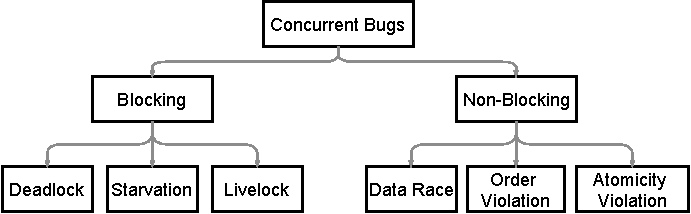
\includegraphics[width=.9\textwidth]{dissertation_intro_bugs.pdf}
\caption{Taxanomy of concurrent bugs}
\label{fig:ch1_concBugs}
\end{figure}

\subsubsection{Concurrent Debugging}
Figure \ref{fig:ch1_concDebugging} displays the general taxonomy of methods for tackling concurrency debugging challenges.
%
\textbf{Testing} exercises the program behavior over a set of inputs (manually written tests) or over the schedule space (feasible interleavings) to detect errors. Although testing effectively reveals flaws of the program, it does not guarantee the program's bug freedom.
\textbf{Model checking} exhaustively test the program to cover possible control flow paths and verify the program properties. However, due to scalability problems, model checking is typically done symbolically and up to a certain bound; thus, they rarely achieve a guarantee.
\textbf{Tracing} collects evidence from program execution, enabling offline analysis of the program's dynamic behavior. Similar to tracing, \textbf{Record and Replay} technique captures a single execution of the target program for later replay and analysis of the program's non-deterministic behavior. Both methods usually incur overhead to the native execution of the program and require sophisticated mechanisms to make them practical for real-world programs and large-scale executions. \textbf{Theorem Proving} techniques, in principle, prove a system to be free of flaws often through verifying type systems. The enormous effort needed to use these tools makes them most appropriate for new implementations of small, critical cores. \textbf{Visualization} techniques provide transparent representations of complex concurrent execution of the program for developers to analyze visually.

In this dissertation, we combine and apply methods from \textit{tracing} (chapters \ref{sec:ch2} and \ref{sec:ch4}), \textit{record and replay} (chapters \ref{sec:ch2},\ref{sec:ch3} and \ref{sec:ch4}), \textit{testing} (chapter \ref{sec:ch4}), and \textit{visualization} (chapters \ref{sec:ch3} and \ref{sec:ch4}) to facilitate the process of concurrent debugging.
\begin{figure}[t]
\centering
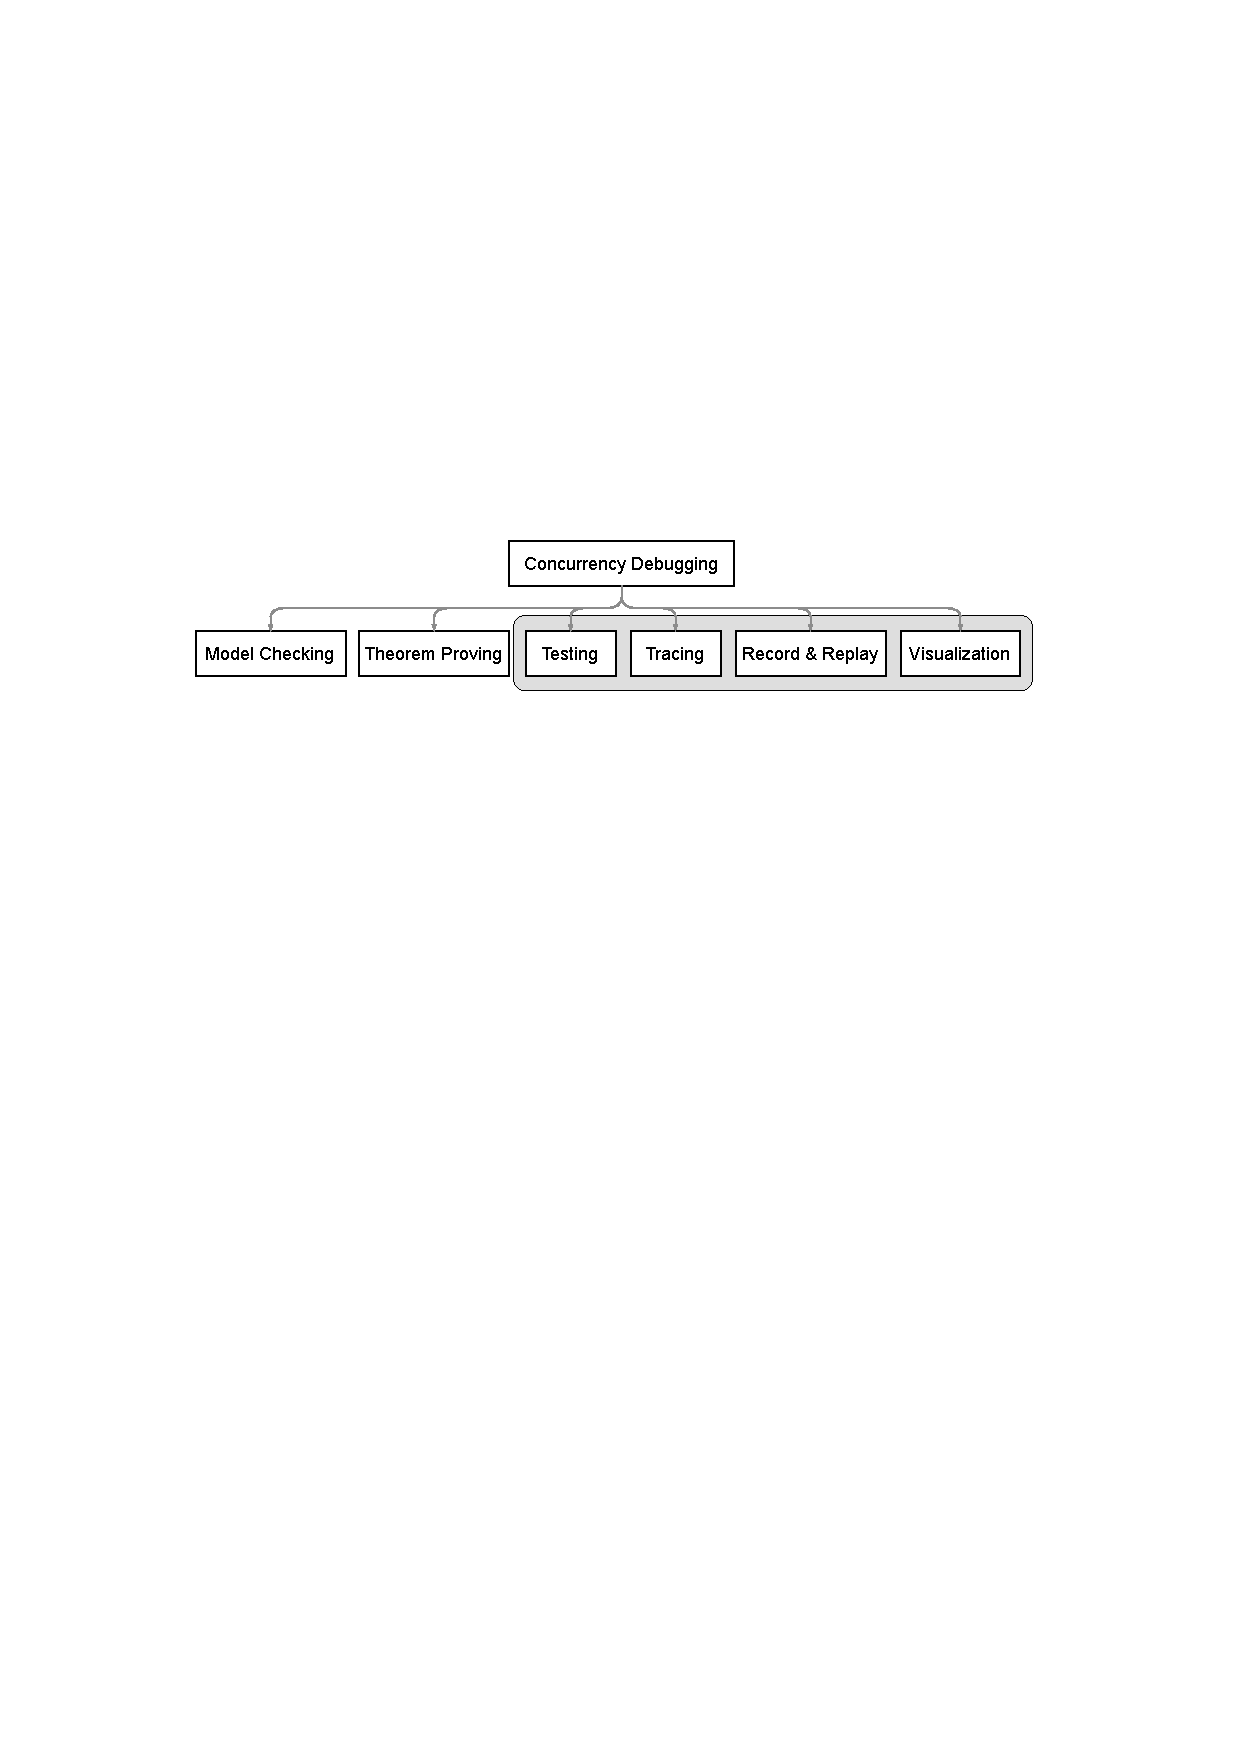
\includegraphics[width=1\textwidth]{dissertation_intro_approaches2.pdf}
\caption{Taxanomy of concurrent debugging approaches. The highlighted area shows the techniques that we employed in this disseration.}
\label{fig:ch1_concDebugging}
\end{figure}



\section{Dissertation Statement}

This dissertation aims to facilitate the concurrent debugging process by providing efficient data collection and effective information retrieval mechanisms to target real-world software and bugs.
%
With that being said, our thesis statement is the following:

\begin{quote}
Efficiently collecting data and systematically analyzing them is essential to gaining insight into the behavior of complex programs and help developers fix the flaws of the program. Also, given the rich set of concurrency primitives in modern languages, one needs to articulate nuanced concurrency coverage metrics and demonstrate their attainment.
\end{quote}

\section{Contributions of the Dissertation}
In this dissertation, we present different contributions to facilitate concurrent debugging using efficient tools and automated frameworks.
%

First, we introduce \parlot (Chapter \ref{sec:ch2}), a new tracing approach that makes it possible to capture the whole-program call-return, call-stack, call-graph, and call-frequency information, including all library calls, for every thread and process of HPC applications at low overhead in both space and time.
%
\parlot is equipped with a new incremental data compression algorithm to drastically reduce the required tracing bandwidth (average of 56 kB/s per core), thus enabling the collection of whole-program traces, which would be infeasible without on-the-fly compression.
%
\parlot can instrument x86 applications at the binary level (regardless of the source language used) to collect whole-program call traces with the compression ratio of up to 21,000.

Second, we present DiffTrace (Chapter \ref{sec:ch3}), a series of automated data abstraction, representation, and visualization techniques that differentiate the collected \parlot traces and narrows the search space down to just a few candidates of buggy traces.
%
In DiffTrace, we employ {\em concept lattices} to amalgamate the collected traces and hierarchically cluster them based on features extracted from the structure of traces.
%
DiffTrace also utilizes the rigorous notion of Nested Loop Representations (NLRs) for summarizing traces and representing loops in a manner that informs the developer engaged in debugging.
%
We evaluate the effectivness of DiffTrace by locating artificial bugs injected to ILCS \cite{ilcs}, a hybrid (MPI + OpenMP) HPC framework.

Third, we illustrate \goat (Chapter \ref{sec:ch4}), a testing and analysis framework for concurrent Go applications that provides for whole-program trace collection (via an enhancement to the standard tracer package) and knowledge discovery about the program's dynamic behavior.
%
We show the effectiveness of controlled preemptions for concurrency bug exposure in the context of a real-world language.
%
We demonstrate the effectivness of \goat by detecting all 68 GoKer \cite{yuan-gobench-cgo21} blocking bugs, many of which are undetected by existing tools.
%
Lastly, we propose a set of coverage requirements to measure testing quality in CSP-like concurrent languages.
The proposed metrics characterize the dynamic behavior of concurrency primitives, enabling measurement of quality and progress of schedule-space exploration.


\section{Organization of the Dissertation}
This dissertation is organized as follows: In Chapter \ref{sec:ch2}, we present the design and evaluation of \parlot, the whole-program tracing mechanism; Chapter \ref{sec:ch3} illustrates the series of trace abstractions and representations towards locating the flaw by clustering and diffing traces; with Chapter \ref{sec:ch4}, we describe the end-to-end analysis and testing framework for concurrent Go applications called \goat, and propose a set of concurrency coverage metrics to measure the quality of schedule space exploration; finally, in Chapter \ref{sec:ch5}, we summarize all the contributions and conclude the dissertation.


%%% -*-LaTeX-*-
\extrafloats{100}

\chapter{Whole-Program Dyamic Tracing}

This chapter is based on the work published at the Workshop on Programming and Performance Visualization Tools (ESPT) 2018 \cite{parlot}.
We present \parlot, a framework for efficient whole-program call tracing for HPC (MPI+X) applications using Intel Pin \cite{pin} dynamic binary isntrumentation that includes following key features: (1) It describes a technique that makes low-overhead on-the-fly compression of whole-program call traces feasible. (2) It presents a new, efficient, incremental trace-compression approach that reduces the trace volume dynamically, which lowers not only the needed bandwidth but also the tracing overhead. (3) It collects all caller/callee relations, call frequencies, call stacks, as well as the full trace of all calls and returns executed by each thread, including in library code. (4) It works on top of existing dynamic binary instrumentation tools, thus requiring neither source-code modifications nor recompilation. (5) It supports program analysis and debugging at the thread, thread-group, and program level.
\parlot establishes that comparable capabilities are currently unavailable. Our experiments with the NAS parallel benchmarks running on the Comet supercomputer with up to 1,024 cores show that ParLoT can collect whole-program function-call traces at an average tracing bandwidth of just 56 kB/s per core.


\section{Introduction}
\label{sec:ch2_intro}
Understanding and debugging HPC programs 
is time-consuming for the user and computationally inefficient.
%
This is especially true when one has to 
track control flow in terms of function calls and returns that may
span library and system codes. 
%
Traditional software engineering quality assurance methods are 
often inapplicable to HPC where concurrency combined with 
large problem scales and sophisticated domain-specific math can make programming 
very challenging. 
%
For example, it took months for scientists to debug an MPI laser-plasma interaction 
code~\cite{hpcdoe}.


HPC bugs may be a combination of both flawed program logic and unspecified or illegal interactions between various concurrency models (e.g., PThreads, MPI, OpenMP, etc.) that coexist in most large applications \cite{hpcdoe}. Moreover, HPC software tends to consume vast amounts of CPU time and hardware resources. Reproducing bugs by rerunning the application is therefore expensive and undesirable. 
%The best hope for debugging lies in being able to efficiently capture detailed execution 
A natural and field-proven approach for debugging is to capture detailed execution traces and compare the traces against corresponding traces from previous (stable) runs~\cite{stat,cstg}.
%
A {\em key requirement} is to do this collection {\em as efficiently as possible}
and in {\em as general and comprehensive a manner} as possible.


Existing tools in this space
do not meet our criteria for efficiency and generality.
%
The highly acclaimed STAT~\cite{stat} tool has helped isolate
bugs based on building equivalence classes of MPI processes and spotting
outliers.
%
We would like to go beyond the capabilities offered by STAT and support
the collection of {\em whole-program} traces that can then be employed
by a  gamut of back-end tools.
%
Also, STAT is usually brought into the picture
when a failure (e.g., a deadlock or hang) is encountered. We would like
to move toward an ``always on'' collection regime, as we cannot anticipate
when a failure will occur -- or, more importantly, {\em whether the failure
will be reproducible.}
%
There are no reported debugging studies on using STAT in
continuous collection (``always on'') mode.
%
In CSTG~\cite{cstg}, the collection is orchestrated by the
user around chosen collection points and employs heavy-weight
unix {\tt backtrace} calls.
%
These again are different from \parlot, where collection points would not be a priori chosen.


The thrust of the work in this paper is to avoid many of the drawbacks of existing
tracing-based tools.
%
We are interested in avoiding
source-code modifications and recompilation --- thus making binary
instrumentation-based tools the only practical and widely deployable option.
%
We also believe in the value
of creating tools that are {\em portable across a 
wide variety of platforms}.
%

%
Our goal is to use \textit{compression} for trace aggregation and to offer 
a generic and low-overhead tracing method that 
(1)~collects dynamic call information during execution (all function calls and returns) for debugging, performance evaluation, phase detection \cite{cbb}, etc.,
(2)~has low overhead, 
(3)~and requires little tracing bandwidth.
%
{\em Providing all these features in a single tool
that operates based on binary instrumentation
is an unsolved problem.}
%
In this paper, we describe a new tracing approach that fulfills these requirements, which we implemented in our proof-of-concept \parlot tool.


%
With \parlot, users can easily build a host of post-processors to examine
executions from many vantage points.
%
For instance, they can write post-processors
to detect unexpected (or ``outlier'') executions.
%
If needed, they can 
drill down and detect abnormal behaviors {\em even in the runtime and
support library stack} such as MPI-level activities.
%
In HPC, it is well-known (especially on newer machines) that bugs are often due to
broken libraries (MPI, OpenMP), a broken runtime, or OS-level activities.
%
Having a single low-overhead tool that can ``X-ray'' an application to this depth is a goal met by \parlot --- a unique feature in today's tool eco-system.

To further motivate the need for whole-program function call
traces, consider the expression {\tt f()+g()}.
%
In C, there is no sequence point associated with the {\tt +}
operator~\cite{sequence-points-in-C}.
%
If these function calls have inadvertent side-effects causing 
failure, it is important to know in which order {\tt f()}
and {\tt g()} were invoked---something that is easy to discern using
\parlot 's traces.
%
One may be concerned that such a tool introduces excessive execution slowdown.
%
\parlot goes to great lengths to minimize these overheads to a level that we believe most users will find acceptable. The mindset is to \textit{``pay a little upfront to dramatically reduce the number of overall debug iterations''}. 

%
As proof of concept, we gathered preliminary results from using the \parlot tracing mechanism to compare different runs.
%
We injected various bugs into the MPI-related functions of ILCS \cite{ilcs}, a parallelization framework for iterative local searches.
%
We ran \parlot on top of executions of buggy and bug-free versions of ILCS and collected traces.
%
Since \parlot's traces maintain the order of the function calls, we were able to split the traces at multiple points of interest and to feed different chunks of traces to a Concept Lattice data structure \cite{clbook} \cite{clconst}. 
%
Having the totally ordered sequence of function calls of the whole program for each active process/thread enabled us to quickly narrow down the search space to locate the cause of the abnormal behavior in the buggy version of ILCS. 

%
This paper does not pursue debugging per se but rather a thorough benchmarking of \parlot. It makes the following main contributions:
%

\begin{itemize}
\item It introduces a new tracing approach that makes it possible to capture the whole-program call-return, call-stack, call-graph, and call-frequency information, including all library calls, for every thread and process of HPC applications at low overhead in both space and time.
\item It describes a new incremental data compression algorithm to drastically reduce the required tracing bandwidth, thus enabling the collection of whole-program traces, which would be infeasible without on-the-fly compression.
\item It presents \parlot, a proof-of-concept tool that implements our compression-based low-overhead tracing approach. \parlot is capable of instrumenting x86 applications at the binary level (regardless of the source language used) to collect whole-program call traces.
\end{itemize}
%
The remainder of this paper is organized as follows. Section \ref{sec:bgreltool} introduces the basic ideas and infrastructure behind \parlot and other tracing tools. Section \ref{sec:design} describes the design of \parlot in detail. Sections \ref{sec:evalmeth} and \ref{sec:results} present our evaluation of different aspects of \parlot and compare it with a similar tool. Section \ref{sec:concl}
concludes the paper with a summary and future work.
% that includes the construction of verification tools that exploit \parlot traces.







\section{Background and Related Work}
\label{sec:ch2_bgreltool}
Recording a log of events during the execution of an application is essential for better understanding the program behavior and, in case of a failure, to locate the problem.
%
Recording this type of information requires instrumentation of the program either at the source-code or the binary-code level.
%
Instrumenting the source code by adding extra libraries and statements to collect the desired information is easy for developers.
%
However, doing so modifies the code and requires recompilation, often involving multiple different tools and complex hierarchies of makefiles and libraries, which can make this approach cumbersome and frustrating for users.
%
Instrumenting an executable at the binary level using a tool is typically easier, faster, and less error prone for most users.
%
Moreover, binary instrumentation is language independent, portable to any system that has the appropriate instrumentation tool installed, and provides machine-level insight into the behavior of the application.
%

\subsection{Binary Instrumentation}
Executables can be instrumented \textit{statically}, where the additional code is inserted into the binary before execution, which results in a persistent modified executable, or \textit{dynamically}, where the modification of the executable is not permanent. In dynamic binary instrumentation, code behavior can be monitored at runtime, making it possible to handle dynamically-generated and self-modifying code. Furthermore, it may be feasible to attach the instrumentation to a running process, which is particularly useful for long-running applications and infinite loops.

Many different tools for investigating application behavior have been designed on top of such Dynamic Binary Instrumentation (DBI) frameworks. For instance, Dyninst~\cite{dyninst} provides a dynamic instrumentation API that gives developers the ability to measure various performance aspects. It is used in tools like Open-SpeedShop~\cite{openss} and TAU~\cite{tau} as well as correctness debuggers like STAT~\cite{stat}. Moreover, VampirTrace~\cite{vampirt} uses it to provide a library for collecting program execution logs. 

Valgrind~\cite{valgrind} is a shadow-value DBI framework that keeps a copy of every register and memory location. It provides developers with the ability to instrument system calls and instructions. Error detectors such as Memcheck~\cite{memcheck} and call-graph generators like \callgrind~\cite{callgrind} are built upon Valgrind.\footnote{Given the absence of tools similar to \parlot, we employ \callgrind
 as a ``close-enough'' tool in our comparisons elaborated in \S\ref{sec:tracing-tools}.
 In this capacity, \callgrind is similar to \parlotm, a variant of \parlot that only collects
 traces from the {\tt main} image. We perform such comparison to have an idea of how we fare
 with respect to one other tool. In \S\ref{sec:results}, we also present a self-assessment of \parlot separately.}

 
%


We implemented \parlot on top of \pin~\cite{pin}, a DBI framework for the IA-32, x86-64, and MIC instruction-set architectures for creating dynamic program analysis tools. There is also version of \pin available for the ARM architecture \cite{pinarm}. \parlot mutates \pin to trace the entry (call) and exit (return) of every executed function. Note that our tracing and compression approaches can equally be implemented on top of other instrumentation tools. For example, PMaC \cite{pmac} is a DBI tool for the PowerPC/AIX architecture upon which \parlot could also be based.


\subsection{Efficient Tracing}
When dealing with large-scale parallel programs, any attempt to capture reasonably frequent events will result in a vast amount of data. Moreover, transferring and storing the data will incur significant overhead. For example, collecting just one byte of information per executed instruction yields on the order of a gigabyte of data per second on a single high-end core. Storing the resulting multi-gigabyte traces from many cores can be a challenge, even on today's large hard disks.

Hence, to be able to capture whole-program call traces, we need a way to decrease the space and runtime overhead. \textit{Compression} can encode the generated data using a smaller number of bits, help
reduce the amount of data movement across the memory hierarchy, and
lower storage and network demands.
%
Although the encoded data will later have to be decoded for analysis, compressing them during tracing enables the collection of {\em whole-program} traces.

The use of compression by itself is not new.
Various performance evaluation tools~\cite{tau,scorep,eventflowgraph} 
already employ compression during the collection
of performance analysis data.
%
Tools such as ScalaTrace~\cite{scalatrace}
also exploit
the repetitive nature of time-step simulations~\cite{freitag}. Aguilar et al. \cite{aguilar} proposed a lossy compression mechanism using the Nami library \cite{gamblinNami} for online MPI tracing. Mohror and Karavanic \cite{mohror} investigated similarity-based trace reduction techniques to store and analyze traces at scale. 


Many performance and debugging tools for HPC applications \cite{stat,taumrnet} rely on mechanisms such as MRNet \cite{mrnet} to accelerate the collection and aggregation of traces based on an overlay network to overcome the challenge of massive data movement and analysis. However, our experiments show that, due to the high compression ratio of \parlot traces, such mechanisms for data movement and aggregation may be unnecessary.

The novelty offered by \parlot lies in the combination of compression
speed, efficacy, and low timing jitter
made possible by its {\em incremental}
lossless compression algorithm, which is
described in \S\ref{sec:design}.
%
It immediately compresses all traced information while the application is running, that is, \parlot does not record the uncompressed trace in memory. 
%
As a result, just a few kilobytes of data need to be written out per thread and per second, thus requiring only a small fraction of the  disk or network bandwidth. 
%
The traces are decompressed later when they are read for offline analysis.
%
From the decompressed full function-call trace, the complete call-graph, 
call-frequency, and caller-callee information can be extracted. 
%
This can be done at the granularity of a thread, a group of threads, or the whole application.
%
We now elaborate on the design of \parlot that makes
these innovations possible.
%--









\section{Design of \parlot}
\label{sec:ch2_design}
Our experimental results in \S\ref{sec:ch2_results} highlight why \textit{compression} is essential to make our approach work.
%
We used \parlot to record a unique 16-bit identifier for every function call and return.
%
Tracing just this small amount of information without compression when running the Mantevo miniapps~\cite{mantevo} on Stampede 1 resulted in about 2 MB/s of data per core on average.
%
Extrapolating this value to all 102,400 cores of Stampede 1 (not counting the accelerators) yields 205 GB/s of trace data, which exceeds the Lustre filesystem's parallel write performance of 150 GB/s.
%
Enabling \parlot's compression algorithm reduced the emitted trace data by a factor of 100 on average, a ratio that is quite stable w.r.t scaling, making it possible to trace full-scale programs while leaving over 98\% of the I/O bandwidth to the application. Therefore, \parlot should also work for codes with higher bandwidth requirements than the ones we tested.

Figure \ref{overview} provides a general overview of \parlot 's workflow.
%
Basic blocks within program executables are {\em dynamically} instrumented before being executed. The collected data are compressed on-the-fly at runtime.
%

\begin{figure}[!t]
\centering
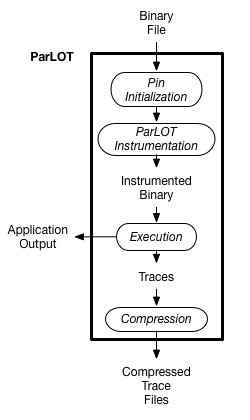
\includegraphics[width=2.2in]{parlot/overview3.png}
\caption{Overview of \parlot}
\label{overview}
\end{figure}


\subsection{Tracing Operation}
\label{subsec:traceOp}

\parlot uses the PIN API as its instrumentation mechanism to gather traces. In particular, it instructs \pin to instrument every thread launch and termination in the application as well as every function entry and exit. The thread-launch instrumentation code initializes the per-thread tracing variables and opens a file into which the trace data from that thread will be written. The thread-termination code finalizes any ongoing compression, flushes out any remaining entries, and closes the trace file. \parlot assigns every static function in each image (main program and all libraries) a unique unsigned 16-bit ID, which it records in a separate file together with the image and function name. This file allows the trace reader to map IDs back to function-name/image pairs.

For every function \emph{entry}, \parlot executes extra code that has access to the thread ID, function ID, and current stack-pointer (SP) value. Based on the SP value, it performs call-stack correction if necessary (see \S\ref{subsec:stack_cor}), adds the new function to a data structure it maintains that holds the call stack (which is separate from the application's runtime stack), and emits the function ID into the trace file via an incremental compression algorithm (see \S\ref{subsec:incr-compr}). All of this is done independently for each thread. Similarly, for every function \emph{exit}, \parlot also executes extra code that has access to the thread ID, function ID, and current SP value. Based on the SP value, it performs call-stack correction if necessary, removes the function from its call-stack data structure, and emits the reserved function ID of zero into the trace file to indicate an exit. As before, this is done via an incremental compression algorithm. We use zero for all exits rather than emitting the function ID and a bit to specify whether it is an entry or exit because using zeros results in more compressible output. This way, half of the values in the trace will be zero.





\subsection{Incremental Compression}
\label{subsec:incr-compr}

\parlot immediately compresses the traced information even before it is written to memory. It does, however, keep a sliding window (circular buffer) of the most recent uncompressed trace events, which is needed by the compressor. It compresses each function ID before the next function ID is known. The conventional approach would be to first record uncompressed function IDs in a buffer and later compress the whole buffer once it fills up. However, this makes the processing time very non-uniform. Whereas almost all function IDs can be recorded very quickly since they just have to be written to the buffer, processing a function ID that happens to fill the buffer takes a long time as it triggers the compression of the entire buffer. This results in sporadic blocking of threads during which time they make no progress towards executing the application code. Initial experiments revealed that such behavior can be detrimental when one thread is polling data from another thread that is currently blocked due to compression. For example, we observed a several order of magnitude increase in entry/exit events of an internal MPI library function when using block-based compression.

To remedy this situation, the compressor must operate incrementally, i.e., each piece of trace data must be compressed when it is generated, without buffering it first, to ensure that there is never a long-latency compression delay. Few existing compression algorithms have been implemented in such a manner because it is more difficult to code up and probably a little slower. Nevertheless, we were able to implement our algorithm (discussed next) in this way so that each trace event is compressed with similar latency.


\subsection{Compression Algorithm}
\label{subsec:compAlg}

We used the CRUSHER framework~\cite{mb-cluster15, mb-space16, mb-sc16, mb-dcc18} to automatically synthesize an effective and fast lossless compression algorithm for our traces. CRUSHER is based on a library of data transformations extracted from various compression algorithms. It combines these transformations in all possible ways to generate algorithm candidates, which it then evaluates on a set of training data. We gathered uncompressed traces from some of the Mantevo miniapps~\cite{mantevo} for this purpose. This evaluation revealed that a particular word-level Lempel-Ziv (LZ) transformation followed by a byte-level Zero-Elimination (ZE) transformation works well. In other words, \parlot 's trace entries, which are two-byte words, are first transformed using LZ. The output is interpreted as a sequence of bytes, which is transformed using ZE for further compression. The output of ZE is written to secondary storage.

LZ implements a variant of the LZ77 algorithm~\cite{LZ}. It uses a 4096-entry hash table to identify the most recent prior occurrence of the current value in the trace. Then it checks whether the three values immediately before that location match the three trace entries just before the current location. If they do not, the current trace entry is emitted and LZ advances to the next entry. If the three values match, LZ counts how many values following the current value match the values following that location. The length of the matching substring is emitted and LZ advances by that many values. Note that all of this is done incrementally. The history of previous trace entries available to LZ for finding matches is maintained in a 64k-entry circular buffer.

ZE emits a bitmap in which each bit represents one input byte. The bits indicate whether the corresponding bytes are zero or not. Following each eight-bit bitmap, ZE emits the non-zero bytes.

As mentioned above, we had to implement the two transformations incrementally to minimize the maximum latency. This required breaking them up into multiple pieces. Depending on the state the compressor is in when the next trace entry needs to be processed, the appropriate piece of code is executed and the state updated. If the LZ code produces an output, which it only does some of the time, then the appropriate piece of the ZE code is executed in a similar manner.


\subsection{PIN and Call-Stack Correction}
\label{subsec:stack_cor}

To be able to decode the trace, i.e., to correctly associate each exit with the function entry it belongs to, our trace reader maintains an identical call-stack data structure. Unfortunately, and as pointed out in the \pin documentation~\cite{pinurl}, it is not always possible to identify all function exits. For example, in optimized code, a function's instructions may be inlined and interleaved with the caller's instructions, making it sometimes infeasible for \pin to identify the exit. As a consequence, we have to ensure that \parlot works correctly even when \pin misses an exit. This is why the SP values are needed.

During tracing, \parlot not only records the function IDs in its call stack but also the associated SP values. This enables it to detect missing exits and to correct the call stack accordingly. Whenever a function is entered, it checks if there is at least one entry in the call stack and, if so, whether its SP value is higher than that of the current SP. If it is lower, we must have missed at least one exit since the runtime stack grows downwards (the SP value decreases with every function entry and increases with every exit). If a missing exit is detected in this manner, \parlot pops the top element from its call stack and emits a zero to indicate a function exit. It repeats this procedure until the stack is empty or its top entry has a sufficiently high SP value. The same call-stack correction technique is applied for every function exit whose SP value is inconsistent. Note that the SP values are only used for this purpose and are not included in the compressed trace.

The result is an internally consistent trace of function entry and exit events, meaning that parsing the trace will yield a correct call stack. This is essential so that the trace can be decoded properly. Moreover, it means that the trace includes exits that truly happened in the application but that were missed by \pin. Note, however, that our call-stack correction is a best-effort approach and may, in rare cases, temporarily not reflect what the application actually did. For example, this can happen for functions that do not create a frame on the runtime stack. When implementing \parlot on top of another DBI framework, call-stack correction may not be needed, resulting in even lower \parlot overhead.


\section{Evaluation Methodology}
\label{sec:ch2_evalmeth}
\subsection{Benchmarks and System}

We performed our evaluations on the MPI-based NAS Parallel Benchmarks (NPB)~\cite{nas}.
%
NPB includes four inputs sizes.
%
To keep the runtimes reasonable, we show results for the class \textit{B} (small-medium) and class \textit{C} (medium-large) inputs.
%

We compiled the NPB codes with the mpicc and mpif77 wrappers of MVAPICH 2.2.1, which are based on icc/ifort 14.0.2 using the prescribed -g and -O1 optimization flags.
%
Quick tests showed that higher optimization levels do not significantly improve the performance.
%

We ran all experiments on Comet at the San Diego Supercomputer Center~\cite{comet}, whose filesystem is NFS and Lustre.
%
Comet has 1944 compute nodes, each of which has dual-socket Intel Xeon E5-2680 v3 processors with a total of 28 cores (14 per socket) and 128 GB of main memory.
%
Note that we only used 16 cores per node as many of the NPB programs require a core count that is a power of two.
%
To study the scaling behavior, we ran experiments on 1, 4, 16 and 64 compute nodes, i.e., on up to 1024 cores.

\subsection{Metrics}

We use the following metrics to quantify and compare the performance of the tracing tools.
%
Unless otherwise noted, all results are based on the median of three identical experiments.
%
\begin{itemize}
\item The \textbf{tracing overhead} is the runtime of the target application when it is being traced divided by the runtime of the same application without tracing.
%
This lower-is-better ratio measures by how much the tracing (and the compression when enabled) slows down the target application.
%
\item The \textbf{tracing bandwidth} is the size of the trace information divided by the application runtime.
%
To make the results easier to compare, we generally list the tracing bandwidth per core, i.e., the tracing bandwidth divided by the number of cores used.
%
This lower-is-better metric is expressed in kilobytes per second (kB/s) per core.
%
It specifies the average needed bandwidth to record the trace data.
%
\item The \textbf{compression ratio} is the size of the uncompressed trace divided by the size of the generated (compressed) trace.
%
This higher-is-better ratio measures the factor by which the compression reduces the trace size.
%
In other words, without compression, the tracing bandwidth would be higher by this factor.
\end{itemize}

\subsection{Tracing Tools}
\label{sec:tracing-tools}

We compare our \parlot tool, implemented on top of \pin 3.5, with \callgrind 3.13.
%
\parlot was compiled with gcc 4.9.2 using \pin 's make system and \callgrind with Valgrind's make system.
%
We created the following versions of \parlot to evaluate different aspects of its design.

% ORIGINAL TABLE
\iffalse
\begin{table}[]
\caption{Overhead added by each tool. Last column is the geometric mean}
\label{comet_sd_pMpAcg_BC_itn_p3.5}\begin{center}
\npdecimalsign{.}
\nprounddigits{1}
\begin{tabular}{lrrrrrrrrr}
\hline
                &   bt &   cg &    ep &    ft &   is &   lu &   mg &   sp &   GM \\
\hline
 pinMain.B.1    & 1.55 & 1.82 &  2.62 &  2.11 & 2.47 & 1.31 & 2.53 & 1.33 & 1.90 \\
 pinMain.B.4    & 1.76 & 1.85 &  1.89 &  1.74 & 1.78 & 1.77 & 1.52 & 1.73 & 1.75 \\
 pinMain.B.16   & 2.15 & 2.58 &  1.99 &  1.89 & 1.78 & 2.73 & 2.43 & 2.15 & 2.19 \\
 pinMain.B.64   & 2.10 & 2.17 &  2.39 &  1.96 & 4.31 & 4.39 & 1.97 & 2.07 & 2.52 \\
 AVG            & 1.89 & 2.10 &  2.22 &  1.92 & 2.58 & 2.55 & 2.11 & 1.82 & 2.09 \\
 pinAll.B.1     & 1.84 & 2.73 &  4.18 &  2.78 & 4.22 & 1.73 & 4.75 & 1.72 & 2.77 \\
 pinAll.B.4     & 2.57 & 3.06 &  3.41 &  2.77 & 2.96 & 2.76 & 2.79 & 2.66 & 2.86 \\
 pinAll.B.16    & 3.52 & 4.20 &  3.39 &  2.94 & 2.83 & 4.30 & 4.46 & 3.65 & 3.62 \\
 pinAll.B.64    & 3.14 & 3.26 &  3.83 &  3.02 & 5.44 & 4.65 & 3.17 & 3.31 & 3.65 \\
 AVG            & 2.77 & 3.31 &  3.70 &  2.88 & 3.86 & 3.36 & 3.79 & 2.83 & 3.23 \\
 callgrind.B.1  & 8.62 & 5.96 &  8.92 & 10.14 & 2.52 & 7.54 & 3.27 & 6.61 & 6.10 \\
 callgrind.B.4  & 6.02 & 3.60 &  2.90 &  3.50 & 1.46 & 5.18 & 1.24 & 5.78 & 3.23 \\
 callgrind.B.16 & 4.28 & 3.26 &  2.24 &  2.17 & 1.70 & 4.62 & 1.81 & 4.34 & 2.84 \\
 callgrind.B.64 & 2.26 & 2.03 &  1.66 &  2.05 & 4.07 & 3.97 & 1.47 & 2.46 & 2.34 \\
 AVG            & 5.29 & 3.71 &  3.93 &  4.46 & 2.44 & 5.33 & 1.95 & 4.80 & 3.63 \\
 pinMain.C.1    & 1.41 & 1.29 &  2.51 &  1.89 & 2.29 & 1.12 & 1.74 & 1.10 & 1.60 \\
 pinMain.C.4    & 1.58 & 1.73 &  1.75 &  1.62 & 1.68 & 1.33 & 1.81 & 1.35 & 1.60 \\
 pinMain.C.16   & 1.82 & 2.38 &  2.46 &  1.51 & 1.80 & 2.18 & 2.36 & 1.80 & 2.01 \\
 pinMain.C.64   & 2.23 & 2.74 &  2.39 &  1.59 & 4.46 & 3.42 & 2.43 & 2.24 & 2.57 \\
 AVG            & 1.76 & 2.04 &  2.28 &  1.65 & 2.56 & 2.01 & 2.08 & 1.62 & 1.94 \\
 pinAll.C.1     & 1.47 & 1.55 &  3.17 &  1.97 & 2.82 & 1.23 & 2.52 & 1.19 & 1.87 \\
 pinAll.C.4     & 1.89 & 2.42 &  2.56 &  2.06 & 2.56 & 1.70 & 3.08 & 1.71 & 2.20 \\
 pinAll.C.16    & 2.69 & 3.47 &  4.07 &  2.14 & 2.80 & 3.18 & 3.98 & 2.54 & 3.04 \\
 pinAll.C.64    & 3.61 & 4.13 &  4.21 &  2.22 & 5.47 & 4.43 & 4.23 & 3.02 & 3.80 \\
 AVG            & 2.42 & 2.89 &  3.50 &  2.10 & 3.41 & 2.63 & 3.45 & 2.11 & 2.73 \\
 callgrind.C.1  & 8.50 & 4.44 & 13.18 & 13.13 & 3.32 & 7.90 & 5.91 & 5.14 & 6.91 \\
 callgrind.C.4  & 8.66 & 4.46 &  4.76 &  6.37 & 1.65 & 6.38 & 2.75 & 6.34 & 4.64 \\
 callgrind.C.16 & 6.86 & 3.91 &  3.11 &  2.76 & 1.79 & 6.40 & 2.14 & 6.09 & 3.69 \\
 callgrind.C.64 & 4.37 & 3.46 &  2.13 &  2.50 & 4.24 & 5.24 & 2.08 & 3.81 & 3.30 \\
 AVG            & 7.10 & 4.07 &  5.79 &  6.19 & 2.75 & 6.48 & 3.22 & 5.34 & 4.63 \\
\hline
\end{tabular}
\npnoround
\end{center}
\end{table}
\fi



\iftrue

\begin{table}[!b]
\caption{Overhead added by each tool}
\label{comet_sd_pMpAcg_BC_itn_p3.5}\begin{center}
\npdecimalsign{.}
\nprounddigits{1}
\scalebox{0.80}{
\begin{tabular}{|c|c|c|n{2}{1}n{2}{1}n{2}{1}n{2}{1}n{2}{1}n{2}{1}n{2}{1}n{2}{1}|n{2}{1}|}
\hline
Input & Tool & \# Nodes  & \multicolumn{1}{c}{bt} & \multicolumn{1}{c}{cg} & \multicolumn{1}{c}{ep} & \multicolumn{1}{c}{ft} & \multicolumn{1}{c}{is} & \multicolumn{1}{c}{lu} & \multicolumn{1}{c}{mg} & \multicolumn{1}{c|}{sp} & \multicolumn{1}{c|}{GM} \\ \hline
\multirow{15}{*}{B} & \multirow{5}{*}{\parlotm} & 1 & 1.55 & 1.82 &  2.62 &  2.11 & 2.47 & 1.31 & 2.53 & 1.33 & 1.90 \\
 &  & 4  & 1.76 & 1.85 &  1.89 &  1.74 & 1.78 & 1.77 & 1.52 & 1.73 & 1.75 \\
 &  & 16  & 2.15 & 2.58 &  1.99 &  1.89 & 1.78 & 2.73 & 2.43 & 2.15 & 2.19 \\
 &  & 64  & 2.10 & 2.17 &  2.39 &  1.96 & 4.31 & 4.39 & 1.97 & 2.07 & 2.52 \\ \cline{3-12}
 &  & AVG & 1.89 & 2.10 &  2.22 &  1.92 & 2.58 & 2.55 & 2.11 & 1.82 & {\boldmath}2.09 \\ \cline{2-12}
 & \multirow{5}{*}{\parlota} & 1 & 1.84 & 2.73 &  4.18 &  2.78 & 4.22 & 1.73 & 4.75 & 1.72 & 2.77 \\
 & & 4     & 2.57 & 3.06 &  3.41 &  2.77 & 2.96 & 2.76 & 2.79 & 2.66 & 2.86 \\
 & & 16    & 3.52 & 4.20 &  3.39 &  2.94 & 2.83 & 4.30 & 4.46 & 3.65 & 3.62 \\
 & & 64    & 3.14 & 3.26 &  3.83 &  3.02 & 5.44 & 4.65 & 3.17 & 3.31 & 3.65 \\ \cline{3-12}
 & & AVG   & 2.77 & 3.31 &  3.70 &  2.88 & 3.86 & 3.36 & 3.79 & 2.83 & {\boldmath}3.23 \\ \cline{2-12}
 & \multirow{5}{*}{\callgrind}  & 1  & 8.62 & 5.96 &  8.92 & 10.14 & 2.52 & 7.54 & 3.27 & 6.61 & 6.10 \\
 & & 4   & 6.02 & 3.60 &  2.90 &  3.50 & 1.46 & 5.18 & 1.24 & 5.78 & 3.23 \\
 & & 16  & 4.28 & 3.26 &  2.24 &  2.17 & 1.70 & 4.62 & 1.81 & 4.34 & 2.84 \\
 & & 64  & 2.26 & 2.03 &  1.66 &  2.05 & 4.07 & 3.97 & 1.47 & 2.46 & 2.34 \\ \cline{3-12}
 & & AVG & 5.29 & 3.71 &  3.93 &  4.46 & 2.44 & 5.33 & 1.95 & 4.80 & {\boldmath}3.63 \\ \hline
 \multirow{15}{*}{C} & \multirow{5}{*}{\parlotm} & 1  & 1.41 & 1.29 &  2.51 &  1.89 & 2.29 & 1.12 & 1.74 & 1.10 & 1.60 \\
 & & 4   & 1.58 & 1.73 &  1.75 &  1.62 & 1.68 & 1.33 & 1.81 & 1.35 & 1.60 \\
 & & 16  & 1.82 & 2.38 &  2.46 &  1.51 & 1.80 & 2.18 & 2.36 & 1.80 & 2.01 \\
 & & 64  & 2.23 & 2.74 &  2.39 &  1.59 & 4.46 & 3.42 & 2.43 & 2.24 & 2.57 \\ \cline{3-12}
 & & AVG & 1.76 & 2.04 &  2.28 &  1.65 & 2.56 & 2.01 & 2.08 & 1.62 & {\boldmath}1.94 \\ \cline{2-12}
 & \multirow{5}{*}{\parlota} & 1 & 1.47 & 1.55 &  3.17 &  1.97 & 2.82 & 1.23 & 2.52 & 1.19 & 1.87 \\
 & & 4   & 1.89 & 2.42 &  2.56 &  2.06 & 2.56 & 1.70 & 3.08 & 1.71 & 2.20 \\
 & & 16  & 2.69 & 3.47 &  4.07 &  2.14 & 2.80 & 3.18 & 3.98 & 2.54 & 3.04 \\
 & & 64  & 3.61 & 4.13 &  4.21 &  2.22 & 5.47 & 4.43 & 4.23 & 3.02 & 3.80 \\ \cline{3-12}
 & & AVG & 2.42 & 2.89 &  3.50 &  2.10 & 3.41 & 2.63 & 3.45 & 2.11 & {\boldmath}2.73 \\ \cline{2-12}
 & \multirow{5}{*}{\callgrind} & 1 & 8.50 & 4.44 & 13.18 & 13.13 & 3.32 & 7.90 & 5.91 & 5.14 & 6.91 \\
 & & 4   & 8.66 & 4.46 &  4.76 &  6.37 & 1.65 & 6.38 & 2.75 & 6.34 & 4.64 \\
 & & 16  & 6.86 & 3.91 &  3.11 &  2.76 & 1.79 & 6.40 & 2.14 & 6.09 & 3.69 \\
 & & 64  & 4.37 & 3.46 &  2.13 &  2.50 & 4.24 & 5.24 & 2.08 & 3.81 & 3.30 \\ \cline{3-12}
 & & AVG & 7.10 & 4.07 &  5.79 &  6.19 & 2.75 & 6.48 & 3.22 & 5.34 & {\boldmath}4.63 \\ \hline
\end{tabular}}
\npnoround
\end{center}
\end{table}

\fi



\begin{itemize}
\item \textbf{\parlotm} is the normal \parlot tool configured to only collect function-call traces from the main image of the application.
\item \textbf{\parlota} is the normal \parlot tool configured to collect function-call traces from all images of the application, including library function calls.
\item \textbf{\pininit} is a crippled version of \parlot from which the tracing code has been removed.
%
The purpose of \pininit is to see how much of the overhead is due to \pin.
\item \textbf{\parlotnc} is the normal \parlot tool but with compression disabled.
%
It writes out the captured data in uncompressed form.
%
The purpose of \parlotnc is to show the performance impact of the compression.
\end{itemize}

It proved surprisingly difficult to find a tool that is similar to \parlot because there appear to be no other tools that generate whole program call traces.
%
In the end, we settled on \callgrind as the most similar tool we could find and used it for our comparisons.
%
\callgrind is based on the Valgrind DBI tool.
%
It collects function-call graphs combined with performance data to show the user what portion of the execution time has been spent in each function.

%%%%%%%%%%%%%%%%%%%%%%%%%%%%%%%%%
% FROM RESULTS - average overhead
%%%%%%%%%%%%%%%%%%%%%%%%%%%%%%%%%

Each \callgrind trace file contains a sequence of function names (or their code) plus numerical data for each function on its caller-callee relationship with other functions.
%
Moreover, it contains cost information for each function in terms of how many machine instructions it read.
%
This information is collected using hardware performance counters.
%
The format of the file is plain ASCII text.
%
Interestingly, all numerical values are expressed relative to previous values, i.e., they are delta (or difference) encoded.
%
This simple form of compression is enabled by default in \callgrind.


\begin{figure}[b]
\centering
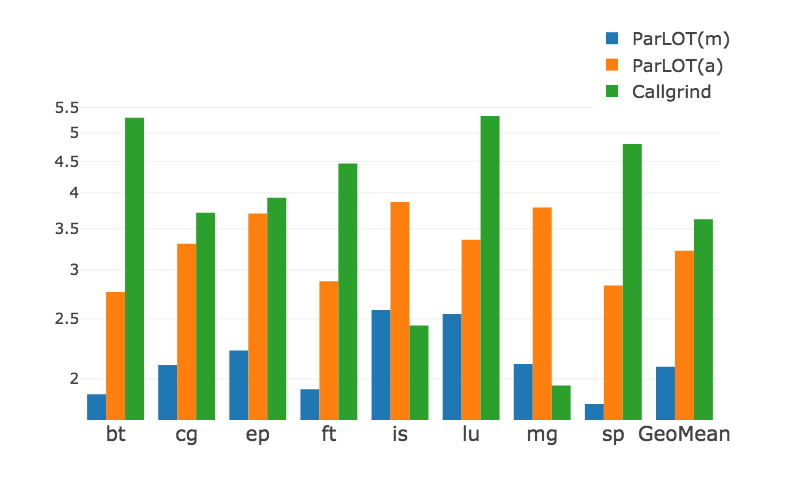
\includegraphics[width=.75\textwidth]{parlot/figs.comet.newMed/comet_chartAvg_sd_B_p3_5.png}
\caption{Average tracing overhead on the NPB applications - Input B}
\label{comet_chartAvg_sd_B_p3_5}
\end{figure}

\begin{figure}[b]
\centering
%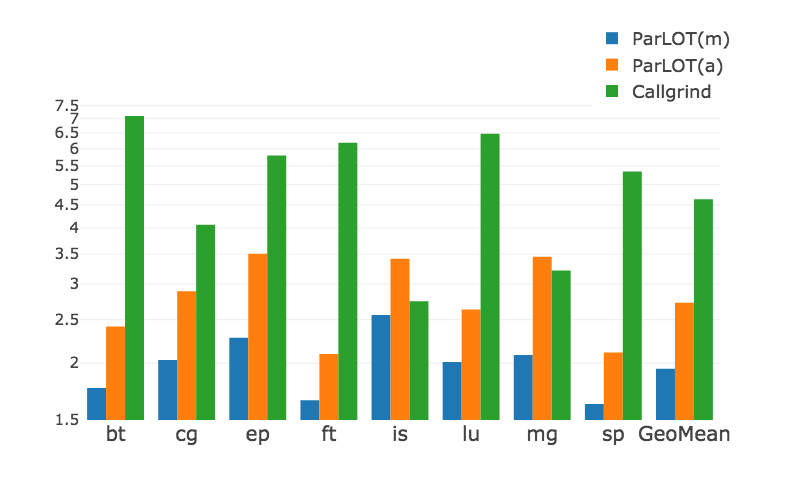
\includegraphics[width=3.4in,height=1.9in]{parlot/figs.comet.newMed/comet_chartAvg_sd_C_p3_5.png}
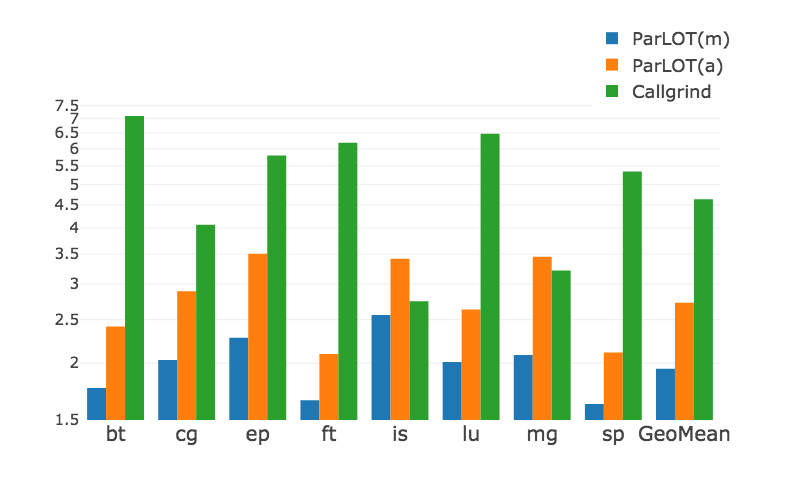
\includegraphics[width=.75\textwidth]{parlot/figs.comet.newMed/comet_chartAvg_sd_C_p3_5.png}
\caption{ Average tracing overhead on the NPB applications - Input C}
\label{comet_chartAvg_sd_C_p3_5}
\end{figure}


We believe the information traced by \callgrind is reasonably similar to the information traced by \parlotm.
%
Whereas \callgrind 's traces include performance data that \parlot does not capture, \parlot records the whole-program call trace, which \callgrind does not capture.
%
The full function-call trace is a strict superset of the call-graph information that \callgrind records because the call graph can be extracted from the function-call trace but not vice versa.
%
In particular, \callgrind cannot recreate the order of the function calls a thread made whereas \parlot can.


\section{Results}
\label{sec:ch2_results}
%%%%%%%%%%%%%%%%%%%%%%%%%%%%%%%%%%%%%
% Tracing Overhead
%%%%%%%%%%%%%%%%%%%%%%%%%%%%%%%%%%%%%

\subsection{Tracing Overhead}
\label{subsec:lowtoh}
\iffalse

\begin{table*}[]
\caption{Req BW}
\label{comet_bw_pMpAcg_BC_itn_p3.5}\begin{center}
\begin{tabular}{lrrrrrrrrr}
\hline
                &    bt &     cg &    ep &    ft &    is &     lu &    mg &     sp &    GM \\
\hline
 pinMain.B.1    &  4.72 &  21.86 &  3.83 &  1.52 &  0.79 &   2.39 &  5.62 &   5.36 &  3.69 \\
 pinMain.B.4    & 14.28 &  41.08 &  1.89 &  3.48 &  2.24 &  21.48 &  6.45 &  15.85 &  8.12 \\
 pinMain.B.16   & 14.31 &  46.59 &  1.45 &  4.86 &  3.40 &  31.79 &  6.53 &  18.55 &  9.41 \\
 pinMain.B.64   & 18.56 &  43.59 &  1.25 &  4.56 &  4.49 &  27.07 &  5.63 &  29.62 &  9.92 \\
 AVG            & 12.97 &  38.28 &  2.10 &  3.60 &  2.73 &  20.68 &  6.06 &  17.35 &  7.79 \\
 pinAll.B.1     & 48.71 &  89.39 & 47.23 & 45.63 & 59.98 &  53.62 & 60.81 &  54.33 & 56.21 \\
 pinAll.B.4     & 61.84 & 101.23 & 45.21 & 55.12 & 53.20 &  71.09 & 54.85 &  73.62 & 62.68 \\
 pinAll.B.16    & 73.95 & 116.87 & 47.37 & 48.88 & 47.79 & 100.91 & 55.80 &  84.61 & 67.97 \\
 pinAll.B.64    & 81.80 & 110.15 & 44.16 & 47.98 & 37.84 & 100.26 & 52.67 &  99.90 & 66.47 \\
 AVG            & 66.58 & 104.41 & 45.99 & 49.40 & 49.70 &  81.47 & 56.03 &  78.12 & 63.33 \\
 callgrind.B.1  &  1.57 &   7.69 &  7.39 &  4.56 & 39.49 &   2.61 & 34.41 &   2.71 &  6.67 \\
 callgrind.B.4  &  6.51 &  16.01 & 22.10 & 15.65 & 45.46 &   8.63 & 45.47 &   7.78 & 16.31 \\
 callgrind.B.16 & 17.20 &  24.62 & 37.42 & 23.84 & 29.87 &  16.23 & 51.49 &  15.81 & 24.93 \\
 callgrind.B.64 & 26.82 &  27.65 & 45.93 & 25.14 & 11.04 &  17.75 & 45.27 &  20.20 & 25.02 \\
 AVG            & 13.03 &  18.99 & 28.21 & 17.30 & 31.47 &  11.30 & 44.16 &  11.62 & 18.23 \\
 pinMain.C.1    &  1.82 &  16.96 &  5.15 &  1.16 &  0.69 &   0.77 &  3.56 &   1.40 &  2.17 \\
 pinMain.C.4    &  7.53 &  44.87 &  3.00 &  2.50 &  2.12 &  20.13 &  7.08 &  13.74 &  7.55 \\
 pinMain.C.16   & 16.30 &  55.04 &  1.84 &  6.10 &  3.35 &  34.09 &  7.24 &  20.68 & 10.70 \\
 pinMain.C.64   & 17.45 &  61.43 &  1.30 &  5.93 &  4.42 &  38.28 &  5.62 &  26.09 & 10.94 \\
 AVG            & 10.77 &  44.58 &  2.82 &  3.92 &  2.65 &  23.32 &  5.88 &  15.48 &  7.84 \\
 pinAll.C.1     & 17.80 &  53.37 & 26.34 & 20.89 & 48.31 &  25.31 & 52.61 &  19.46 & 29.99 \\
 pinAll.C.4     & 51.78 &  95.84 & 36.80 & 43.82 & 51.40 &  58.39 & 54.18 &  65.77 & 55.15 \\
 pinAll.C.16    & 75.38 & 121.03 & 44.29 & 61.39 & 46.90 & 101.05 & 56.49 & 101.32 & 71.37 \\
 pinAll.C.64    & 80.63 & 135.19 & 43.49 & 46.28 & 37.09 & 117.87 & 54.05 &  99.02 & 68.99 \\
 AVG            & 56.40 & 101.36 & 37.73 & 43.09 & 45.93 &  75.66 & 54.33 &  71.39 & 56.38 \\
 callgrind.C.1  &  0.40 &   3.09 &  1.96 &  1.05 & 14.60 &   0.70 &  6.96 &   0.75 &  1.85 \\
 callgrind.C.4  &  1.78 &   8.87 &  7.74 &  4.48 & 31.74 &   2.82 & 21.03 &   2.78 &  6.41 \\
 callgrind.C.16 &  6.01 &  15.82 & 22.86 & 10.75 & 26.50 &   7.45 & 39.05 &   6.96 & 13.72 \\
 callgrind.C.64 & 14.32 &  19.56 & 35.75 & 12.17 & 11.07 &  11.86 & 40.69 &  12.83 & 17.39 \\
 AVG            &  5.63 &  11.84 & 17.08 &  7.11 & 20.98 &   5.71 & 26.93 &   5.83 &  9.84 \\
\hline
\end{tabular}
\end{center}
\end{table*}

\fi


\iftrue

\begin{table*}[]
\caption{ Required bandwidth per core (kB/s) }
\label{comet_bw_pMpAcg_BC_itn_p3.5}\begin{center}
\npdecimalsign{.}
\nprounddigits{1}
\scalebox{0.90}{
\begin{tabular}{|c|c|c|n{3}{1}n{3}{1}n{3}{1}n{3}{1}n{3}{1}n{3}{1}n{3}{1}n{3}{1}|n{3}{1}|}
\hline
Input & Tool & \# Nodes  & \multicolumn{1}{c}{bt} & \multicolumn{1}{c}{cg} & \multicolumn{1}{c}{ep} & \multicolumn{1}{c}{ft} & \multicolumn{1}{c}{is} & \multicolumn{1}{c}{lu} & \multicolumn{1}{c}{mg} & \multicolumn{1}{c|}{sp} & \multicolumn{1}{c|}{GM} \\ \hline
\multirow{15}{*}{B} & \multirow{5}{*}{\parlotm} & 1 &  4.72 &  21.86 &  3.83 &  1.52 &  0.79 &   2.39 &  5.62 &   5.36 &  3.69 \\
 & & 4                                               & 14.28 &  41.08 &  1.89 &  3.48 &  2.24 &  21.48 &  6.45 &  15.85 &  8.12 \\
 & & 16                                              & 14.31 &  46.59 &  1.45 &  4.86 &  3.40 &  31.79 &  6.53 &  18.55 &  9.41 \\
 & & 64                                              & 18.56 &  43.59 &  1.25 &  4.56 &  4.49 &  27.07 &  5.63 &  29.62 &  9.92 \\ \cline{3-12} 
 & & AVG                                             & 12.97 &  38.28 &  2.10 &  3.60 &  2.73 &  20.68 &  6.06 &  17.35 &  {\boldmath}7.79  \\ \cline{2-12} 
 & \multirow{5}{*}{\parlota} & 1 & 48.71 &  89.39 & 47.23 & 45.63 & 59.98 &  53.62 & 60.81 &  54.33 & 56.21 \\
 & & 4                            & 61.84 & 101.23 & 45.21 & 55.12 & 53.20 &  71.09 & 54.85 &  73.62 & 62.68 \\
 & & 16                           & 73.95 & 116.87 & 47.37 & 48.88 & 47.79 & 100.91 & 55.80 &  84.61 & 67.97 \\
 & & 64                           & 81.80 & 110.15 & 44.16 & 47.98 & 37.84 & 100.26 & 52.67 &  99.90 & 66.47 \\ \cline{3-12} 
 & & AVG                          & 66.58 & 104.41 & 45.99 & 49.40 & 49.70 &  81.47 & 56.03 &  78.12 & {\boldmath}63.33 \\ \cline{2-12} 
 & \multirow{5}{*}{\callgrind}  & 1  &  1.57 &   7.69 &  7.39 &  4.56 & 39.49 &   2.61 & 34.41 &   2.71 &  6.67  \\
 & & 4                              &  6.51 &  16.01 & 22.10 & 15.65 & 45.46 &   8.63 & 45.47 &   7.78 & 16.31  \\
 & & 16                             & 17.20 &  24.62 & 37.42 & 23.84 & 29.87 &  16.23 & 51.49 &  15.81 & 24.93  \\
 & & 64                             & 26.82 &  27.65 & 45.93 & 25.14 & 11.04 &  17.75 & 45.27 &  20.20 & 25.02  \\ \cline{3-12} 
 & & AVG                            & 13.03 &  18.99 & 28.21 & 17.30 & 31.47 &  11.30 & 44.16 &  11.62 & {\boldmath}18.23  \\ \hline
 \multirow{15}{*}{C} & \multirow{5}{*}{\parlotm} & 1  &  1.82 &  16.96 &  5.15 &  1.16 &  0.69 &   0.77 &  3.56 &   1.40 &  2.17  \\
 & & 4                                                 &  7.53 &  44.87 &  3.00 &  2.50 &  2.12 &  20.13 &  7.08 &  13.74 &  7.55  \\
 & & 16                                                & 16.30 &  55.04 &  1.84 &  6.10 &  3.35 &  34.09 &  7.24 &  20.68 & 10.70  \\
 & & 64                                                & 17.45 &  61.43 &  1.30 &  5.93 &  4.42 &  38.28 &  5.62 &  26.09 & 10.94  \\ \cline{3-12} 
 & & AVG                                               & 10.77 &  44.58 &  2.82 &  3.92 &  2.65 &  23.32 &  5.88 &  15.48 &  {\boldmath}7.84  \\ \cline{2-12} 
 & \multirow{5}{*}{\parlota} & 1 & 17.80 &  53.37 & 26.34 & 20.89 & 48.31 &  25.31 & 52.61 &  19.46 & 29.99 \\
 & & 4                            & 51.78 &  95.84 & 36.80 & 43.82 & 51.40 &  58.39 & 54.18 &  65.77 & 55.15 \\
 & & 16                           & 75.38 & 121.03 & 44.29 & 61.39 & 46.90 & 101.05 & 56.49 & 101.32 & 71.37 \\
 & & 64                           & 80.63 & 135.19 & 43.49 & 46.28 & 37.09 & 117.87 & 54.05 &  99.02 & 68.99 \\ \cline{3-12}
 & & AVG                          & 56.40 & 101.36 & 37.73 & 43.09 & 45.93 &  75.66 & 54.33 &  71.39 & {\boldmath}56.38  \\ \cline{2-12} 
 & \multirow{5}{*}{\callgrind} & 1 &  0.40 &   3.09 &  1.96 &  1.05 & 14.60 &   0.70 &  6.96 &   0.75 &  1.85  \\
 & & 4                            &  1.78 &   8.87 &  7.74 &  4.48 & 31.74 &   2.82 & 21.03 &   2.78 &  6.41  \\
 & & 16                           &  6.01 &  15.82 & 22.86 & 10.75 & 26.50 &   7.45 & 39.05 &   6.96 & 13.72  \\
 & & 64                           & 14.32 &  19.56 & 35.75 & 12.17 & 11.07 &  11.86 & 40.69 &  12.83 & 17.39  \\ \cline{3-12}
 & & AVG                          &  5.63 &  11.84 & 17.08 &  7.11 & 20.98 &   5.71 & 26.93 &   5.83 &  {\boldmath}9.84  \\ \hline
\end{tabular}}
\end{center}
\end{table*}

\fi


%%%%%%%%%%%%%%%%%%%%%%%%%%%%%%%%%
% FROM RESULTS - average bandwidth
%%%%%%%%%%%%%%%%%%%%%%%%%%%%%%%%%
\begin{figure}[t]
\centering
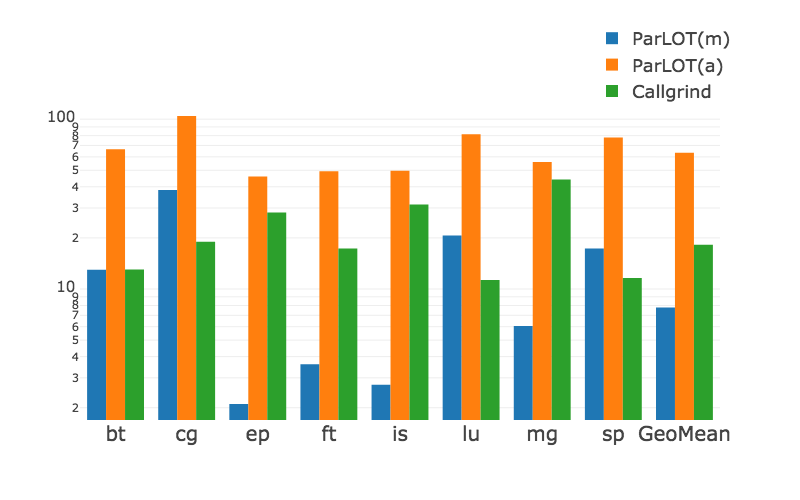
\includegraphics[width=3.4in,height=1.9in]{parlot/figs.comet.newMed/comet_chartAvg_bw_B_p3_5.png}
\caption{  Average required bandwidth per core (kB/s) on the NPB applications - Input B}
\label{comet_chartAvg_bw_B_p3_5}
\end{figure}

\begin{figure}[t]
\centering
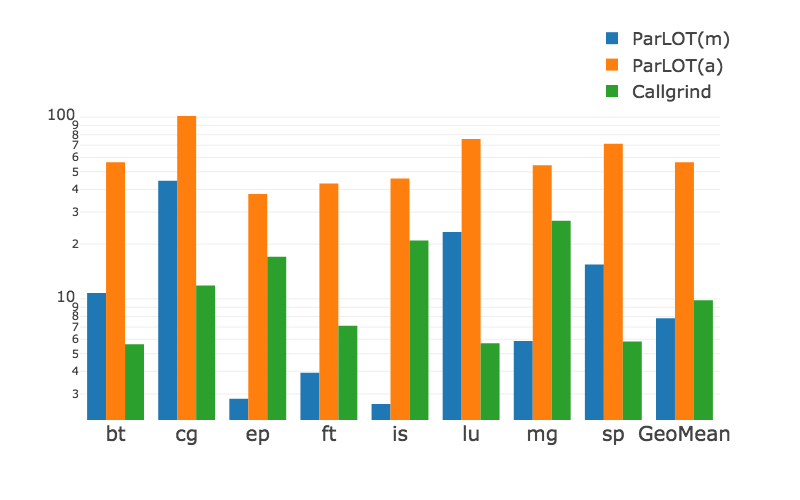
\includegraphics[width=3.4in,height=1.9in]{parlot/figs.comet.newMed/comet_chartAvg_bw_C_p3_5.png}
\caption{ Average required bandwidth per core (kB/s) on the NPB applications - Input C}
\label{comet_chartAvg_bw_C_p3_5}
\end{figure}

%%%%%%%%%%%%%%%%%%%%%%%%%%%%%%%%%
% ENDDDD
%%%%%%%%%%%%%%%%%%%%%%%%%%%%%%%%%

Table \ref{comet_sd_pMpAcg_BC_itn_p3.5} shows the tracing overhead of \parlotm, \parlota, and \callgrind on each application of the NPB benchmark suite for different node counts. The last column of the table lists the geometric mean over all eight programs. The AVG rows show the average over the four node counts.


On average, both \parlotm and \parlota outperform \callgrind. The bolded numbers in Table \ref{comet_sd_pMpAcg_BC_itn_p3.5} for input C show that the average overhead is 1.94 for \parlotm, 2.73 for \parlota, and 4.63 for \callgrind. Figures \ref{comet_chartAvg_sd_B_p3_5} and \ref{comet_chartAvg_sd_C_p3_5} show these results in visual form.


The key takeaway point is that the overhead of \parlot is roughly a factor of two to three, which we believe users may be willing to accept, for example, if it helps them debug their applications. This is promising especially when considering how detailed the collected trace information is and that most of the overhead is due to \pin (see \S\ref{subsec:pinit}). Note that \parlot 's overhead is typically lower than that of \callgrind, which collects less information.

The overhead of \parlot increases as we scale the applications to more compute nodes. However, the increase is quite small. Going from 16 to 1024 cores, a 64-fold increase in parallelism, only increases the average overhead by between 1.3- and 2.1-fold. In contrast, \callgrind 's overhead decreases with increasing node count, making it more scalable. Having said that, \callgrind 's overhead is larger for the C inputs whereas \parlot 's overhead is larger for the smaller B inputs. In other words, \parlot scales better to larger inputs than \callgrind.

\parlot 's scaling behavior can be explained by correlating it with the expected function-call frequency. When distributing a fixed problem size over more cores, each core receives less work. As a consequence, less time is spent in the functions that process the work, resulting in more function calls per time unit, which causes more work for \parlot. In contrast, when distributing a larger problem size over the same number of cores, each core receives more work. Hence, more time is spent in the functions that process the work, resulting in fewer function calls per time unit, which causes less work for \parlot and therefore less tracing overhead. Hence, we believe \parlot 's overhead to be even lower on long-running inputs, which is where our tracing technique is needed the most.


In summary, \parlot 's overhead is in the single digits for all evaluated applications and configurations, including for 1024-core runs. It appears to scale reasonably to larger node counts and well to larger problem sizes.

\subsection{Required Bandwidth}
\label{subsec:lowbw}

Table \ref{comet_bw_pMpAcg_BC_itn_p3.5}, Fig.  \ref{comet_chartAvg_bw_B_p3_5} and Fig. \ref{comet_chartAvg_bw_C_p3_5} show how much trace bandwidth each tool
requires
during the application execution.
%
On average, \parlotm requires less bandwidth than
\callgrind, especially for smaller inputs.
%
\parlota's bandwidth is much higher as it collects call information from all
images and not just the main image like \parlotm does.

We see that the required bandwidth for different input sizes of the NPB applications are almost equal in \parlot. According to the NPB documentation, the number of iterations for inputs B and C are the same for all applications. They only differ in the number of elements or the grid size. It is clear that the required bandwidth of \parlot is independent of the problem size, unlike \callgrind, where the input size has a linear impact on the results.

%
%%%%%%%%%%%%%%%%%%%%%%%%%%%%%%%%%
% FROM RESULTS - average compression ratio
%%%%%%%%%%%%%%%%%%%%%%%%%%%%%%%%%
\begin{figure}[t]
\centering
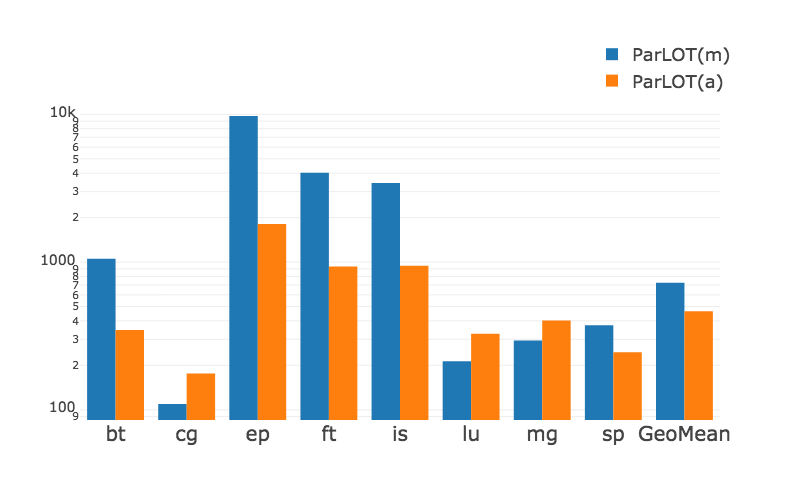
\includegraphics[width=3.2in,height=1.9in]{parlot/figs.comet.newMed/comet_chartAvg_cr_B_p3_5.png}
\caption{ Average compression ratio of \parlot on the NPB applications - Input B}
\label{comet_chartAvg_cr_B_p3_5}
\end{figure}

\begin{figure}[t]
\centering
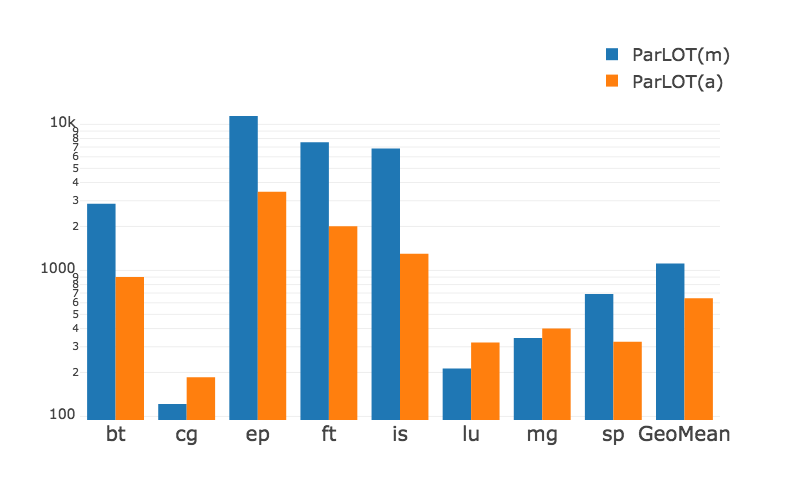
\includegraphics[width=3.2in,height=1.9in]{parlot/figs.comet.newMed/comet_chartAvg_cr_C_p3_5.png}
\caption{ Average compression ratio of \parlot on the NPB applications - Input C}
\label{comet_chartAvg_cr_C_p3_5}
\end{figure}
%%%%%%%%%%%%%%%%%%%%%%%%%%%%%%%%%
% ENDDDD
%%%%%%%%%%%%%%%%%%%%%%%%%%%%%%%%%



\iffalse
\begin{table}[]
\caption{Compression Ratio}
\label{comet_cr_pMpA_BC_itn_p3.5}\begin{center}
\begin{tabular}{lrrrrrrrrr}
\hline
              &      bt &     cg &       ep &       ft &       is &     lu &     mg &      sp &      GM \\
\hline
 pinMain.B.1  & 3035.93 &  94.35 & 12456.18 & 12173.49 &  9718.38 & 167.72 &  99.08 &  878.27 & 1255.17 \\
 pinMain.B.4  &  586.64 &  82.48 & 10368.41 &  1737.09 &   909.20 & 140.29 & 254.95 &  338.16 &  559.36 \\
 pinMain.B.16 &  346.66 & 113.28 &  8563.85 &  1077.35 &  1200.57 & 178.98 & 387.63 &  123.02 &  496.83 \\
 pinMain.B.64 &  252.24 & 147.78 &  7611.04 &  1122.62 &  1907.95 & 366.80 & 437.31 &  152.91 &  591.11 \\
 AVG          & 1055.37 & 109.47 &  9749.87 &  4027.64 &  3434.03 & 213.45 & 294.74 &  373.09 &  725.62 \\
 pinAll.B.1   &  514.51 & 137.41 &  3335.77 &  1226.74 &   543.18 & 314.63 & 260.87 &  303.88 &  500.21 \\
 pinAll.B.4   &  315.71 & 137.21 &  1266.92 &   436.15 &   316.16 & 287.25 & 329.57 &  199.66 &  330.70 \\
 pinAll.B.16  &  226.86 & 181.58 &  1246.66 &  1026.53 &   927.09 & 299.30 & 469.29 &  171.52 &  430.39 \\
 pinAll.B.64  &  329.23 & 247.30 &  1394.07 &  1043.94 &  1984.62 & 410.32 & 548.47 &  307.16 &  597.55 \\
 AVG          &  346.58 & 175.88 &  1810.86 &   933.34 &   942.76 & 327.88 & 402.05 &  245.56 &  464.71 \\
 pinMain.C.1  & 8618.95 & 111.16 & 13067.96 & 21335.57 & 21856.49 & 350.03 & 247.44 & 1977.43 & 2371.35 \\
 pinMain.C.4  & 1910.64 & 110.45 & 12418.66 &  6520.34 &  2256.56 & 112.77 & 267.98 &  472.68 &  928.16 \\
 pinMain.C.16 &  580.79 & 133.24 & 11017.36 &  1239.31 &  1347.88 & 164.47 & 396.86 &  143.13 &  582.78 \\
 pinMain.C.64 &  322.83 & 131.92 &  9154.99 &  1065.12 &  1896.25 & 223.69 & 465.74 &  168.89 &  585.74 \\
 AVG          & 2858.30 & 121.69 & 11414.74 &  7540.09 &  6839.30 & 212.74 & 344.50 &  690.53 & 1117.01 \\
 pinAll.C.1   & 2579.37 & 181.76 &  7376.96 &  5143.08 &  1520.42 & 408.21 & 314.77 &  650.73 & 1107.37 \\
 pinAll.C.4   &  448.61 & 161.32 &  3194.58 &  1062.94 &   527.34 & 274.70 & 319.35 &  237.43 &  477.42 \\
 pinAll.C.16  &  285.05 & 185.74 &  1765.49 &   588.86 &  1106.34 & 273.63 & 467.35 &  141.69 &  426.92 \\
 pinAll.C.64  &  290.00 & 214.68 &  1512.89 &  1237.30 &  2038.72 & 329.04 & 496.21 &  270.83 &  565.82 \\
 AVG          &  900.76 & 185.88 &  3462.48 &  2008.05 &  1298.21 & 321.39 & 399.42 &  325.17 &  644.38 \\
\hline
\end{tabular}
\end{center}
\end{table}

\fi


\iftrue

\begin{table}[]
\caption{ Compression ratio }
\label{comet_cr_pMpA_BC_itn_p3.5}\begin{center}
\npdecimalsign{.}
\nprounddigits{1}
\scalebox{0.7}{
\begin{tabular}{|c|c|c|N{5}{1}N{5}{1}N{5}{1}N{5}{1}N{5}{1}N{5}{1}n{5}{1}n{5}{1}|n{5}{1}|}
\hline
Input & Tool & \# Nodes  & \multicolumn{1}{c}{bt} & \multicolumn{1}{c}{cg} & \multicolumn{1}{c}{ep} & \multicolumn{1}{c}{ft} & \multicolumn{1}{c}{is} & \multicolumn{1}{c}{lu} & \multicolumn{1}{c}{mg} & \multicolumn{1}{c|}{sp} & \multicolumn{1}{c|}{GM} \\ \hline
\multirow{10}{*}{B} & \multirow{5}{*}{\parlotm} & 1 & 3035.93 &  94.35 & 12456.18 & 12173.49 &  9718.38 & 167.72 &  99.08 &  878.27 & 1255.17 \\
 & & 4                                               &  586.64 &  82.48 & 10368.41 &  1737.09 &   909.20 & 140.29 & 254.95 &  338.16 &  559.36 \\
 & & 16                                              &  346.66 & 113.28 &  8563.85 &  1077.35 &  1200.57 & 178.98 & 387.63 &  123.02 &  496.83 \\
 & & 64                                              &  252.24 & 147.78 &  7611.04 &  1122.62 &  1907.95 & 366.80 & 437.31 &  152.91 &  591.11 \\ \cline{3-12}
 & & AVG                                             & 1055.37 & 109.47 &  9749.87 &  4027.64 &  3434.03 & 213.45 & 294.74 &  373.09 &  {\boldmath}725.62  \\ \cline{2-12}
 & \multirow{5}{*}{\parlota} & 1 &  514.51 & 137.41 &  3335.77 &  1226.74 &   543.18 & 314.63 & 260.87 &  303.88 &  500.21 \\
 & & 4                            &  315.71 & 137.21 &  1266.92 &   436.15 &   316.16 & 287.25 & 329.57 &  199.66 &  330.70 \\
 & & 16                           &  226.86 & 181.58 &  1246.66 &  1026.53 &   927.09 & 299.30 & 469.29 &  171.52 &  430.39 \\
 & & 64                           &  329.23 & 247.30 &  1394.07 &  1043.94 &  1984.62 & 410.32 & 548.47 &  307.16 &  597.55 \\ \cline{3-12}
 & & AVG                          &  346.58 & 175.88 &  1810.86 &   933.34 &   942.76 & 327.88 & 402.05 &  245.56 &  {\boldmath}464.71 \\ \hline
 \multirow{10}{*}{C} & \multirow{5}{*}{\parlotm} & 1  & 8618.95 & 111.16 & 13067.96 & 21335.57 & 21856.49 & 350.03 & 247.44 & 1977.43 & 2371.35  \\
 & & 4                                                 & 1910.64 & 110.45 & 12418.66 &  6520.34 &  2256.56 & 112.77 & 267.98 &  472.68 &  928.16  \\
 & & 16                                                &  580.79 & 133.24 & 11017.36 &  1239.31 &  1347.88 & 164.47 & 396.86 &  143.13 &  582.78  \\
 & & 64                                                &  322.83 & 131.92 &  9154.99 &  1065.12 &  1896.25 & 223.69 & 465.74 &  168.89 &  585.74  \\ \cline{3-12}
 & & AVG                                               & 2858.30 & 121.69 & 11414.74 &  7540.09 &  6839.30 & 212.74 & 344.50 &  690.53 & {\boldmath}1117.01  \\ \cline{2-12}
 & \multirow{5}{*}{\parlota} & 1 & 2579.37 & 181.76 &  7376.96 &  5143.08 &  1520.42 & 408.21 & 314.77 &  650.73 & 1107.37 \\
 & & 4                            &  448.61 & 161.32 &  3194.58 &  1062.94 &   527.34 & 274.70 & 319.35 &  237.43 &  477.42 \\
 & & 16                           &  285.05 & 185.74 &  1765.49 &   588.86 &  1106.34 & 273.63 & 467.35 &  141.69 &  426.92 \\
 & & 64                           &  290.00 & 214.68 &  1512.89 &  1237.30 &  2038.72 & 329.04 & 496.21 &  270.83 &  565.82 \\ \cline{3-12}
 & & AVG                          &  900.76 & 185.88 &  3462.48 &  2008.05 &  1298.21 & 321.39 & 399.42 &  325.17 &  {\boldmath}644.38 \\ \cline{2-12} \hline
\end{tabular}}
\npnoround
\end{center}
\end{table}

\fi




\begin{figure}[t]
\centering
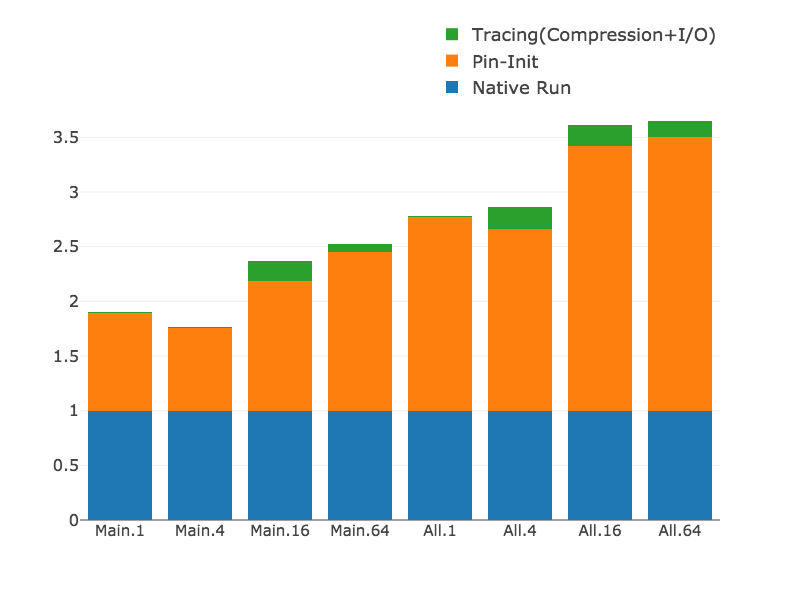
\includegraphics[width=3.1in,height=1.9in]{parlot/figs.comet.newMed/comet_chartDet_B_wc_byTool_p3_5.png}
\caption{ Tracing overhead breakdown - Input B}
\label{comet_chartDet_B_wc_byTool_p3_5}
\end{figure}


\begin{figure}[t]
\centering
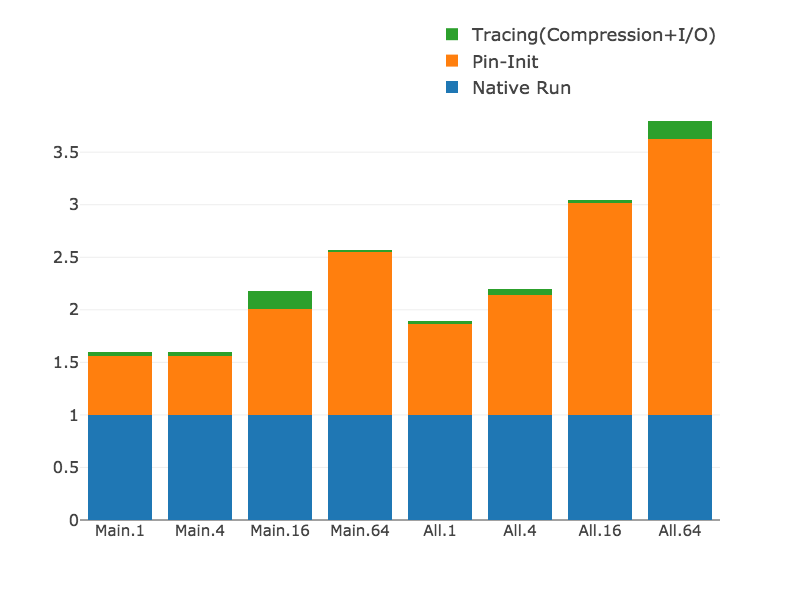
\includegraphics[width=3.1in,height=1.9in]{parlot/figs.comet.newMed/comet_chartDet_C_wc_byTool_p3_5.png}
\caption{ Tracing overhead breakdown - Input C}
\label{comet_chartDet_C_wc_byTool_p3_5}
\end{figure}



\begin{figure}[t]
\centering
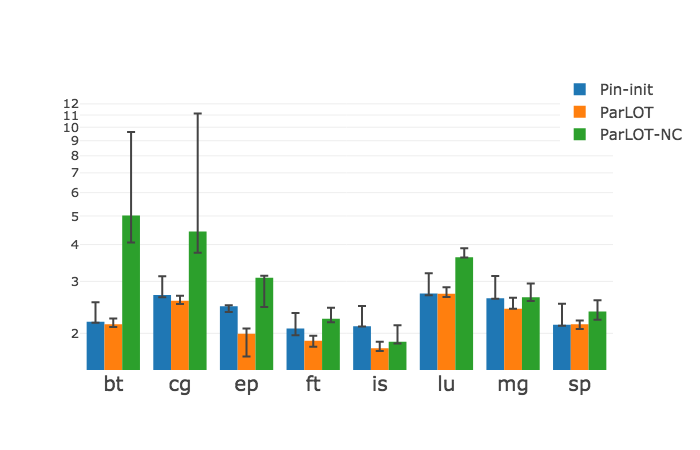
\includegraphics[width=3.2in,height=1.9in]{parlot/figs.comet.newMed/comet_BX2_Main_16_B_p3_5.png}
\caption{ Variability of \parlotm overhead on 16 nodes - Input B}
\label{comet_BX2_Main_16_B_p3_5}
\end{figure}


%%%%%%%%%%%%%%%%%%%%%%%%%%%%%%%%%%%%%%%%%%%%%%%%%%%%%%%%%%%%%%%%%%%%%%%%%%%%%%%%%%

\subsection{Compression Ratio}
\label{subsec:cr}
Table \ref{comet_cr_pMpA_BC_itn_p3.5} shows the compression ratios for all configurations and inputs.
%
On average, \parlot stores between half a kilobyte and a kilobyte of trace information in a single byte.
%
We observe that the
average compression ratio for \parlota on input C is 644.3, and its
corresponding required bandwidth from Table
\ref{comet_bw_pMpAcg_BC_itn_p3.5} is 56.4 kB/s.
%
This means \parlot can
collect \textbf{more than 36 MB} worth of data per core per second
while only needing 56 kB/s of the system bandwidth, {\em leaving the rest of the available bandwidth to the application.}
%
In comparison, \callgrind
collects \textbf{less than 100 kB} of data but still adds more
overhead compared to either \parlota or \parlotm .
%
The average amount of trace data that can be collected by \parlota is
\textbf{360x} (85x for \parlotm) larger than that for \callgrind.
%
In the best observed case, the compression ratio of
\parlot exceeds 21000.
%
This is particularly impressive because it was achieved with relatively low overhead and incremental
on-the-fly compression.
%
Generally, the compression ratios of \parlotm are higher than those of \parlota because the variety of distinct function calls on the main image is smaller than when tracing all images, thus compression performs better on \parlotm.
Also by looking at Fig. \ref{comet_chartAvg_bw_B_p3_5}, Fig. \ref{comet_chartAvg_bw_C_p3_5}, Fig. \ref{comet_chartAvg_cr_B_p3_5} and Fig. \ref{comet_chartAvg_cr_C_p3_5}, we find EP to have the highest compression ratio of the NPB applications. At the same time, it has the minimum required bandwidth. The opposite is true for CG, which exhibits the lowest compression ratio and the highest required bandwidth. CG is a conjugate gradient method with irregular memory accesses and communications whereas EP is an embarrassingly parallel random number generator. CG's whole-program trace contains a larger number of distinct calls and more complex patterns than that of EP, thus resulting in a higher bandwidth and lower compression ratio.
%

\parlot's compression mechanism works better on larger input sizes because larger inputs tend to result in longer streams of similar function calls (e.g., a call that is made for every processed element).



\subsection{Overheads}
\label{subsec:pinit}
Tables \ref{comet_wo_det_Main_all_B_p3.5} and
\ref{comet_wo_det_All_all_B_p3.5} present the average overhead added to each
application for different versions of \parlot.
%
The last row of these two tables
presents the geometric mean.
%
This information captures how much each
phase of \parlot slows down the native execution.

\begin{table}[]
\caption{Tracing overhead of versions of \parlotm - Input B}
\begin{center}
\label{comet_wo_det_Main_all_B_p3.5}
\scalebox{0.5}{
\begin{tabular}{|c|c|rrr|rrr|rrr|rrr|}
\hline
\multicolumn{1}{|l|}{\multirow{2}{*}{\textbf{Input: B}}} & \multicolumn{1}{r|}{Nodes :}    & \multicolumn{3}{c|}{1}  & \multicolumn{3}{c|}{4} & \multicolumn{3}{c|}{16}  & \multicolumn{3}{c|}{64} \\ \cline{2-14}
\multicolumn{1}{|l|}{} & \multicolumn{1}{r|}{Detail Tools:} & \multicolumn{1}{c}{\pininit} & \multicolumn{1}{c}{\parlot} & \multicolumn{1}{c|}{\parlotnc} & \multicolumn{1}{c}{\pininit} & \multicolumn{1}{c}{\parlot} & \multicolumn{1}{c|}{\parlotnc} & \multicolumn{1}{c}{\pininit} & \multicolumn{1}{c}{\parlot} & \multicolumn{1}{c|}{\parlotnc} & \multicolumn{1}{c}{\pininit} & \multicolumn{1}{c}{\parlot} & \multicolumn{1}{c|}{\parlotnc} \\
\hline
\multirow{9}{*}{Main} &     bt  &  1.5  &  1.5  &   5.6  &  1.7  &  1.7  &  5.0  &  2.1  &  2.1  &  5.0  &  1.8  &  2.1  &  3.5 \\
 &  cg  &  1.7  &  1.8  &   2.3  &  1.8  &  1.8  &  2.6  &  2.7  &  2.5  &  4.4  &  2.3  &  2.1  &  4.6 \\
 &  ep  &  2.9  &  2.6  &  20.4  &  1.9  &  1.8  &  5.3  &  2.4  &  1.9  &  3.0  &  2.6  &  2.3  &  2.6 \\
 &  ft  &  1.8  &  2.1  &   6.1  &  1.7  &  1.7  &  2.7  &  2.0  &  1.8  &  2.2  &  2.1  &  1.9  &  2.1 \\
 &  is  &  2.4  &  2.4  &   4.8  &  1.7  &  1.7  &  2.0  &  2.1  &  1.7  &  1.8  &  4.5  &  4.3  &  5.7 \\
 &  lu  &  1.3  &  1.3  &   1.4  &  1.7  &  1.7  &  2.2  &  2.7  &  2.7  &  3.6  &  3.0  &  4.3  &  6.1 \\
 &  mg  &  2.5  &  2.5  &   2.7  &  1.5  &  1.5  &  1.5  &  2.6  &  2.4  &  2.6  &  1.9  &  1.9  &  1.8 \\
 &  sp  &  1.3  &  1.3  &   2.4  &  1.7  &  1.7  &  3.5  &  2.1  &  2.1  &  2.3  &  1.9  &  2.0  &  2.5 \\
\cline{2-14}
 &  GM  &  1.8  &  1.9  &   4.1  &  1.7  &  1.7  &  2.9  &  2.3  &  2.1  &  3.0  &  2.4  &  2.5  &  3.3 \\
\hline
\end{tabular} }

\end{center}
\end{table}








\ignore{--
\begin{table*}[]
\caption{Tracing overhead of different \parlot versions - Input B - Main image}
\begin{center}
\label{comet_wo_det_Main_all_B_p3.5}
\scalebox{0.78}{
\begin{tabular}{|c|c|rrr|rrr|rrr|rrr|}
\hline
\multicolumn{1}{|l|}{\multirow{2}{*}{\textbf{Input: B}}} & \multicolumn{1}{r|}{Nodes :}    & \multicolumn{3}{c|}{1}  & \multicolumn{3}{c|}{4} & \multicolumn{3}{c|}{16}  & \multicolumn{3}{c|}{64} \\ \cline{2-14}
\multicolumn{1}{|l|}{} & \multicolumn{1}{r|}{Detail Tools:} & \multicolumn{1}{c}{\pininit} & \multicolumn{1}{c}{\parlot} & \multicolumn{1}{c|}{\parlotnc} & \multicolumn{1}{c}{\pininit} & \multicolumn{1}{c}{\parlot} & \multicolumn{1}{c|}{\parlotnc} & \multicolumn{1}{c}{\pininit} & \multicolumn{1}{c}{\parlot} & \multicolumn{1}{c|}{\parlotnc} & \multicolumn{1}{c}{\pininit} & \multicolumn{1}{c}{\parlot} & \multicolumn{1}{c|}{\parlotnc} \\
\hline
\multirow{9}{*}{Main} &  bt  &  1.50  &  1.55  &   5.62  &  1.74  &  1.76  &  5.06  &  2.19  &  2.15  &  5.02  &  1.83  &  2.10  &  3.52 \\
 &  cg  &  1.75  &  1.82  &   2.38  &  1.84  &  1.85  &  2.64  &  2.70  &  2.58  &  4.43  &  2.32  &  2.17  &  4.64 \\
 &  ep  &  2.96  &  2.62  &  20.48  &  1.99  &  1.89  &  5.38  &  2.47  &  1.99  &  3.09  &  2.68  &  2.39  &  2.66 \\
 &  ft  &  1.87  &  2.11  &   6.17  &  1.75  &  1.74  &  2.79  &  2.08  &  1.89  &  2.24  &  2.18  &  1.96  &  2.14 \\
 &  is  &  2.47  &  2.47  &   4.82  &  1.79  &  1.78  &  2.07  &  2.11  & 1.78  &  1.87  &  4.51  &  4.31  &  5.71 \\
 &  lu  &  1.32  &  1.31  &   1.44  &  1.75  &  1.77  &  2.25  &  2.73  &  2.73  &  3.62  &  3.05  &  4.39  &  6.13 \\
 &  mg  &  2.56  &  2.53  &   2.79  &  1.56  &  1.52  &  1.59  &  2.63  &  2.43  &  2.65  &  1.95  &  1.97  &  1.85 \\
 &  sp  &  1.34  &  1.33  &   2.43  &  1.73  &  1.73  &  3.58  &  2.14  &  2.15  &  2.37  &  1.95  &  2.07  &  2.54 \\
\cline{2-14}
 &  GM  &  1.89  &  1.90  &   4.10  &  1.77  &  1.75  &  2.92  &  2.37  &  2.19  &  3.00  &  2.45  &  2.52  &  3.33 \\
\hline
\end{tabular} }

\end{center}
\end{table*}
}


\begin{table}[]
\caption{Tracing overhead of versions of \parlota - Input B}
\begin{center}
\label{comet_wo_det_All_all_B_p3.5}
\scalebox{0.78}{
\begin{tabular}{|c|c|rrr|rrr|rrr|rrr|}
\hline
\multicolumn{1}{|l|}{\multirow{2}{*}{\textbf{Input: B}}} & \multicolumn{1}{r|}{Nodes :}    & \multicolumn{3}{c|}{1}  & \multicolumn{3}{c|}{4} & \multicolumn{3}{c|}{16}  & \multicolumn{3}{c|}{64} \\ \cline{2-14}
\multicolumn{1}{|l|}{} & \multicolumn{1}{r|}{Detail Tools:} & \multicolumn{1}{c}{\pininit} & \multicolumn{1}{c}{\parlot} & \multicolumn{1}{c|}{\parlotnc} & \multicolumn{1}{c}{\pininit} & \multicolumn{1}{c}{\parlot} & \multicolumn{1}{c|}{\parlotnc} & \multicolumn{1}{c}{\pininit} & \multicolumn{1}{c}{\parlot} & \multicolumn{1}{c|}{\parlotnc} & \multicolumn{1}{c}{\pininit} & \multicolumn{1}{c}{\parlot} & \multicolumn{1}{c|}{\parlotnc} \\
\hline
\multirow{9}{*}{All} &  bt  &  1.7  &  1.8  &   6.1  &  2.3  &  2.5  &  6.1  &  3.2  &  3.5  &   9.0  &  2.8  &  3.1  &   7.5 \\
 &  cg  &  2.6  &  2.7  &   3.8  &  2.8  &  3.0  &  4.4  &  4.0  &  4.2  &  11.3  &  3.3  & 3.2  &  10.3 \\
 &  ep  &  4.3  &  4.1  &  22.2  &  3.1  &  3.4  &  7.1  &  3.1  &  3.3  &   4.5  &  4.1  & 3.8  &   4.1 \\
 &  ft  &  2.8  &  2.7  &   6.8  &  2.6  &  2.7  &  3.8  &  2.8  &  2.9  &   3.6  &  3.1  &  3.0  &   3.5 \\
 &  is  &  4.4  & 4.2  &   7.0  &  2.8  &  2.9  &  3.4  &  2.9  &  2.8  &   3.2  &  5.3  &  5.4  &   8.8 \\
 &  lu  &  1.7  &  1.7  &   2.3  &  2.5  &  2.7  &  4.8  &  3.9  &  4.3  &  10.4  &  4.4  &  4.6  &  23.4 \\
 &  mg  &  4.8  &  4.7  &   5.3  &  2.5  &  2.7  &  3.0  &  4.3  &  4.4  &   5.2  &  2.7  &  3.1  &   3.2 \\
 &  sp  &  1.7  &  1.7  &   3.0  &  2.4  &  2.6  &  5.0  &  3.2  &  3.6  &   5.6  &  2.7  &  3.3  &  11.6 \\
\cline{2-14}
 &  GM  &  2.7  & 2.7  &   5.5  &  2.6  &  2.8  &  4.5  &  3.4  &  3.6  &   6.0  &  3.5  &  3.6  &   7.4 \\
\hline
\end{tabular} }

\end{center}
\end{table}












\ignore{--

\begin{table}[]
\caption{Tracing overhead of different \parlot versions - Input B}
\begin{center}
\label{comet_wo_det_All_all_B_p3.5}
\scalebox{0.78}{
\begin{tabular}{|c|c|rrr|rrr|rrr|rrr|}
\hline
\multicolumn{1}{|l|}{\multirow{2}{*}{\textbf{Input: B}}} & \multicolumn{1}{r|}{Nodes :}    & \multicolumn{3}{c|}{1}  & \multicolumn{3}{c|}{4} & \multicolumn{3}{c|}{16}  & \multicolumn{3}{c|}{64} \\ \cline{2-14}
\multicolumn{1}{|l|}{} & \multicolumn{1}{r|}{Detail Tools:} & \multicolumn{1}{c}{\pininit} & \multicolumn{1}{c}{\parlot} & \multicolumn{1}{c|}{\parlotnc} & \multicolumn{1}{c}{\pininit} & \multicolumn{1}{c}{\parlot} & \multicolumn{1}{c|}{\parlotnc} & \multicolumn{1}{c}{\pininit} & \multicolumn{1}{c}{\parlot} & \multicolumn{1}{c|}{\parlotnc} & \multicolumn{1}{c}{\pininit} & \multicolumn{1}{c}{\parlot} & \multicolumn{1}{c|}{\parlotnc} \\
\hline
\multirow{9}{*}{All} &  bt  &  1.76  &  1.84  &   6.11  &  2.39  &  2.57  &  6.11  &  3.22  &  3.52  &   9.02  &  2.87  &  3.14  &   7.55 \\
 &  cg  &  2.69  &  2.73  &   3.80  &  2.86  &  3.06  &  4.48  &  4.07  &  4.20  &  11.38  &  3.33  & 3.26  &  10.39 \\
 &  ep  &  4.36  &  4.18  &  22.20  &  3.14  &  3.41  &  7.16  &  3.12  &  3.39  &   4.55  &  4.18  & 3.83  &   4.16 \\
 &  ft  &  2.80  &  2.78  &   6.85  &  2.65  &  2.77  &  3.82  &  2.82  &  2.94  &   3.66  &  3.15  &  3.02  &   3.57 \\
 &  is  &  4.40  & 4.22  &   7.04  &  2.85  &  2.96  &  3.42  &  2.91  &  2.83  &   3.24  &  5.38  &  5.44  &   8.81 \\
 &  lu  &  1.70  &  1.73  &   2.39  &  2.54  &  2.76  &  4.88  &  3.96  &  4.30  &  10.47  &  4.45  &  4.65  &  23.41 \\
 &  mg  &  4.83  &  4.75  &   5.37  &  2.51  &  2.79  &  3.07  &  4.32  &  4.46  &   5.22  &  2.73  &  3.17  &   3.26 \\
 &  sp  &  1.70  &  1.72  &   3.01  &  2.46  &  2.66  &  5.06  &  3.27  &  3.65  &   5.67  &  2.77  &  3.31  &  11.65 \\
\cline{2-14}
 &  GM  &  2.78  & 2.77  &   5.59  &  2.66  &  2.86  &  4.58  &  3.42  &  3.62  &   6.02  &  3.51  &  3.65  &   7.41 \\
\hline
\end{tabular} }

\end{center}
\end{table}
}



%%%%%%%%%%%%%%%%%%%%%%%%%%%%%%%%%%%%%%%%%%%%%%%%%%%%%%%%%%%%%

\begin{figure}[t]
\centering
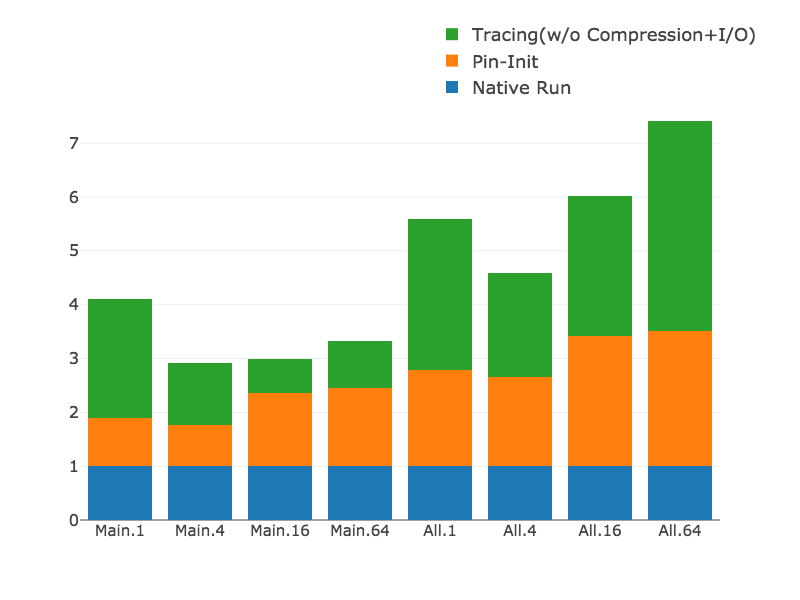
\includegraphics[width=3in,height=1.95in]{parlot/figs.comet.newMed/comet_chartDet_B_woc_byTool_p3_5.png}
\caption{\parlotnc tracing overhead breakdown - Input B}
\label{comet_chartDet_B_woc_byTool_p3_5}
\end{figure}

\begin{figure}[t]
\centering
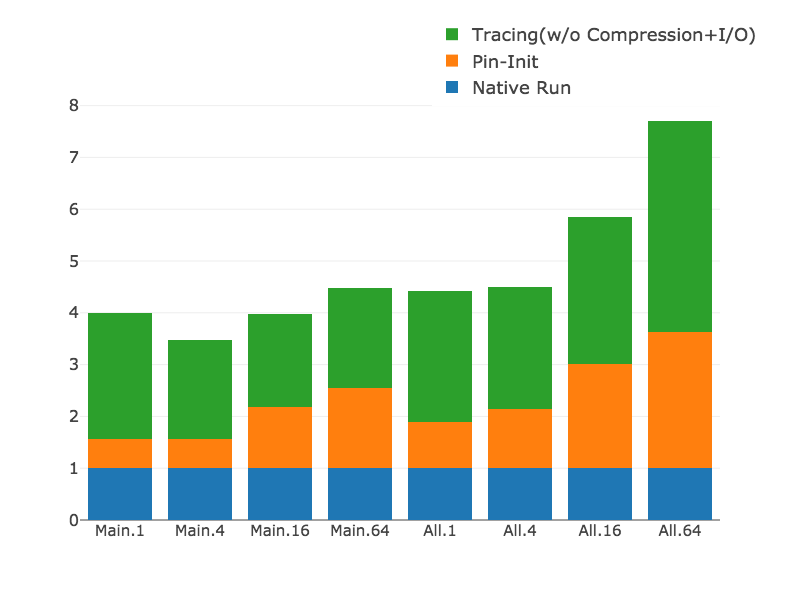
\includegraphics[width=3in,height=1.95in]{parlot/figs.comet.newMed/comet_chartDet_C_woc_byTool_p3_5.png}
\caption{ \parlotnc tracing overhead breakdown - Input C}
\label{comet_chartDet_C_woc_byTool_p3_5}
\end{figure}

In general, one
expects the following inequality to hold:
 the overhead of \pininit should be less than that of \parlot
, which should be less than that of \parlotnc.
%
This is not always the case because of the non-deterministic runtimes of the applications.
%
In fact, the variability across three runs of each experiment
is shown in Fig. \ref{comet_BX2_Main_16_B_p3_5}
where we present the minimum, maximum and median overheads.
%
These
overheads are for input size B and 16 nodes.
%
This variability explains the seeming inconsistencies in  Tables
\ref{comet_wo_det_Main_all_B_p3.5} and
\ref{comet_wo_det_All_all_B_p3.5}.


On average, \pininit adds
an overhead of 3.28  and \parlota adds an overhead of 3.42.
%
This means that \textbf{almost 96\%
of \parlota's overhead is due to \pin}.
%
The results of \parlotm and
other inputs follow the same pattern
as shown in Fig. \ref{comet_chartDet_B_wc_byTool_p3_5} and \ref{comet_chartDet_C_wc_byTool_p3_5}.
%
The overhead that \parlot (excluding the overhead of \pininit) {\em adds}
to the applications is very small.
%
If we were to switch to a different
instrumentation tool that is not as general as \pin but more
lightweight, the overhead would potentially reduce drastically. \\


\subsection{Compression Impact}
\label{subsec:compact}

Fig. \ref{comet_chartDet_B_woc_byTool_p3_5} and Fig. \ref{comet_chartDet_C_woc_byTool_p3_5} show the  overhead breakdown of \parlotnc, which illustrate the impact of compression. They also highlight the importance of incorporating compression directly in the tracing tool.
%
On average, \parlotnc slows down the application execution almost \textbf{2x} more than \parlota.
%
The average overhead
across Table \ref{comet_wo_det_All_all_B_p3.5} for \parlota is \textbf{3.4}.
%
The  corresponding factor for \parlotnc is \textbf{6.6}.
%
The numbers of \parlotm and input C  follow the same pattern. For example, \parlotnc slows down the application execution almost \textbf{1.66x} more than \parlotm.
%

Clearly, compression not only lowers the storage requirement but also the overhead. This is important as it shows that the extra computation to perform the compression is more than amortized by the reduction in the amount of data that need to be written out.
%

This result validates our approach and highlights that incremental, on-the-fly compression is likely essential to make whole-program tracing possible at low overhead.


\section{Discussion and Conclusion}
\label{sec:ch2_concl}

In this paper, 
we present \parlot, a portable low overhead dynamic
binary instrumentation-based
whole-program
tracing approach that can support a variety of 
dynamic program analyses, including debugging.
%
Key properties of \parlot include its on-the-fly trace collection and
compression that reduces timing jitter, I/O bandwidth, and storage requirements to such a degree that whole-program call/return traces can be collected efficiently even at scale. 

We evaluate various versions of \parlot
created by disabling/enabling compression, not collecting any traces, etc.
%
In order to provide an intuitive comparison against a well known tool,
we also compare \parlot to \callgrind.
%
Our metrics include the tracing overhead, required bandwidth, achieved compression ratio, initialization overhead, and the 
overall impact of compression.
%
Detailed evaluations on the NAS parallel benchmarks running on
up to 1024 cores establish the merit of our tool and our design decisions. 
\parlot can collect more than 36 MB worth of data per core per second while 
only needing 56 kB/s of bandwidth and slowing down the 
application by 2.7x on average.
%
These results are highly promising in terms of supporting 
whole program tracing and debugging, in particular when considering that most of the overhead is due to the DBI tool and not \parlot.


The traces collected by \parlot cut through the entire stack of heterogeneous
(MPI, OpenMP, PThreads) calls. 
%
This permits a designer to project these traces onto specific
APIs of interest during program analysis, visualization, and debugging.
%


A number of improvements to \parlot remain to be made.
%
These include allowing users to selectively trace at specific
interfaces: doing so can further increase compression efficiency
by reducing the variety of function calls to be handled by
the compressor.
%
We also discuss the need to bring down initialization overheads, i.e.,
by switching to a less general-purpose DBI tool.
%



\section*{Acknowledgment}

This research was supported by the NSF. We thank our colleague Dr. Hari Sundar from the University of Utah who provided insight and expertise that greatly assisted the research. We also thank the Texas Advanced Computing Center (TACC) and the San Diego Supercomputer Center (SDSC) for the infrastructure they provided for running our experiments.

 
%--end


%%% -*-LaTeX-*-

\chapter{Whole-Program Trace Analysis}
\label{sec:ch3}

This chapter is based on the work published at the 2019 IEEE International Conference on Cluster Computing \cite{diffTrace}\footnote{\copyright 2019 IEEE. Adapted, with permission, from S. Taheri, I. Briggs, M. Burtscher and G. Gopalakrishnan, ``DiffTrace: Efficient Whole-Program Trace Analysis and Diffing for Debugging'', 2019 IEEE International Conference on Cluster Computing (CLUSTER), 2019, pp. 1-12, doi: 10.1109/CLUSTER.2019.8891027}.
%
We present a tool called \textbf{DiffTrace} that approaches debugging via {\em whole program} tracing and
diffing of typical and erroneous traces.
%
After collecting these traces, a user-configurable front-end filters out irrelevant function calls and then summarizes loops in the retained function calls based on state-of-the-art loop extraction algorithms.
%
Information about these loops is inserted into concept lattices, which we use to compute salient dissimilarities to narrow down bugs.
%
DiffTrace is a clean start that addresses debugging features missing in existing approaches.
%
Our experiments on an MPI/OpenMP program called ILCS and initial measurements on LULESH, a DOE miniapp, demonstrate the advantages of the proposed debugging approach.

\section{Introduction}
\label{sec:ch3_intro}
Debugging high-performance computing code
remains a challenge at all levels of scale.
%
Conventional HPC debuggers~\cite{ddt,totalview}
excel at many tasks such as examining the execution
state of a complex simulation in detail
and allowing the developer to re-execute
the program close to the point of failure.
%
However, they do not provide a good understanding
of why a program version that worked earlier
failed upon upgrade or feature addition.
%
Innovative solutions are needed to highlight the
salient differences between two executions in a manner
that makes debugging easier as well as more systematic.
%
A recent study conducted under the auspices of the
DOE~\cite{hpcdoe}
provides a comprehensive survey
of existing debugging tools.
%
It classifies them under
four software organizations (serial, multithreaded,
multi-process, and hybrid), six
method types (formal methods, static analysis, dynamic
analysis, nondeterminism control, anomaly detection,
and parallel debugging), and lists a total of 30 specific
tools.
%
Despite this abundance of activity and tools, many
significant problems remain to be solved before debugging
{\em can be approached by the HPC community as a collaborative
activity} so that HPC developers can extend a common
framework.


Almost all debugging approaches seek to find outliers (``unexpected
executions'') amongst thousands of running processes and threads.
%
The approach taken by most existing tools is to
look for symptoms in a specific bug-class that they cover.
%
Unfortunately,
this approach calls for a programmer having a good guess of what
the underlying problem might be,
and to then pick the right set of tools to deploy.
%
If the guess is wrong, the programmer has no choice but to
refine their guess
and look for bugs in another class,
re-executing the application and hoping for
better luck with another tool.
%
This iterative loop of re-execution followed by applying a
best-guess tool for the suspected bug class can potentially consume
large amounts of execution cycles and wastes an
expert developer's time.
%
More glaring is the fact that these tools must recreate the
execution traces yet again: they do not have means to hand off
these traces to another tool or cooperate in symbiotic ways.



We cannot collect all relevant pieces of information
necessary to detect all possible bug classes such as
resource leaks, deadlocks, and data races.
%
Each such bug requires its attributes to be kept.
%
Also, debugging is not fully automatable (it is
an undecidable problem in general) and must involve human thinking:
at least to reconcile what is observed against the deeper application-level semantics.
%
However, (1)~we believe that it is still possible to collect one standard set
of data and use it to make an initial triage in such
a way that it can guide a later, deeper debugging phase to locate
which of the finer bug gradations (e.g., resource leaks or races) brought
the application down.
%
Also, (2)~we believe that it is possible to engage the human {\em with respect
to understanding structured presentations of information}.



Our DiffTrace framework addresses both issues.
%
The common set of data it uses is a {\em whole program
function call trace} collected per process/thread.
%
DiffTrace relies on
novel ways to diff a normal trace and a fault-laden trace to guide the
debugging engineer closer to the bug.
%
While our work has not (yet) addressed situations in
which millions of threads and thousands of processes run
for days before they produce an error,
we strongly believe that we can get there
once we understand the pros and cons of our initial
implementation of the DiffTrace tool, which is described in this paper.
%
The second issue is handled in DiffTrace by offering a novel
collection of modalities for understanding program execution diffs.
%
We now elaborate on these points by addressing the following three problems.



\subsection{Problem 1 -- Collecting Whole-Program Heterogeneous Function-Call Traces
Efficiently\/} Not only must we have the ability
to record function calls and returns at one
API such as MPI, increasingly we must collect calls/returns at multiple
interfaces (e.g., OpenMP, PThreads, and even inner levels such as TCP).
%
The growing use of heterogeneous parallelization necessitates that we
understand MPI and OpenMP activities (for example) to locate cross-API
bugs that are often missed by other tools.
%
Sometimes, these APIs contain the actual error (as opposed to the user code), and it would be attractive to have this debugging ability.


{\em Solution to Problem 1:\/}
In DiffTrace, we choose Pin-based whole program binary tracing, with
tracing filters that allow the designer to collect a suitable mixture of API
calls/returns.
%
We realize this facility using
ParLOT, a tool designed by us and published earlier~\cite{parlot}.
%
In our research, we have thus far demonstrated the advantage of
ParLOT with respect to collecting both MPI and OpenMP traces
from a {\em single run of a hybrid MPI/OpenMP program}.
%
We demonstrate that, from this single type of trace, it is possible
to pick out MPI-level bugs and/or OpenMP-level bugs.
%
While whole-program tracing
may sound extremely computation and storage intensive, ParLOT employs
lightweight on-the-fly compression techniques to keep these overheads low.
%
It achieves compression ratios exceeding 21,000~\cite{parlot},
thus making this approach practical, demanding
only a few kilobytes per second per core of bandwidth.


\subsection{Problem 2 -- Need to Generalize Techniques for Outlier Detection\/}
Given that outlier detection is central to debugging,
it is essential to use efficient representations of the traces
to be able to systematically compute
{\em distances} between them without
involving human reasoning.
%
The representation must also be versatile enough to
be able to ``diff'' the traces
with respect to {\em an extensible number of vantage points}.
%
These vantage points could be diffing traces concerning process-level activities,
thread-level activities, a combination thereof,
or even finite sequences of process/thread calls (say, to locate {\em changes}
in caller/callee relationships).


{\em Solution to Problem 2:\/}
DiffTrace employs {\em concept lattices} to amalgamate the collected traces.
%
Concept lattices have previously been employed in HPC to perform structural
clustering of process behaviors~\cite{weberStructural} to present performance data more
meaningfully to users.
%
The authors of that paper use the notion of {\em Jaccard distances}
to cluster performance results that are closely related to process structures
(determined based on caller/callee relationships).
%
In DiffTrace, we employ incremental algorithms for building and maintaining
concept lattices from the ParLOT-collected traces.
%
In addition to Jaccard distances, in our work, we also perform hierarchical
clustering of traces and provide a tunable threshold for outlier detection.
%
We believe that these uses of concept lattices and refinement approaches
for outlier detection are new in HPC debugging.


\subsection{Problem 3 -- Loop Summarization\/}
Most programs spend most of their time in loops.
%
Therefore, it is important to employ state-of-the-art algorithms for
loop extraction from execution traces.
%
It is also important
to be able to diff two executions with respect to changes in their looping behaviors.
%
In our experience, presenting such changes using good visual metaphors
tends to highlight many bug types immediately.


{\em Solution to Problem 3:\/}
DiffTrace utilizes the rigorous notion of Nested Loop Representations (NLRs) for
summarizing traces and representing loops.
%
Each repetitive loop structure is given an identifier, and nested loops are
expressed as repetitions of this identifier exponentiated (as with regular
expressions).
%
This approach to summarizing loops can help manifest
bugs where the program does not hang or crash but nevertheless
runs differently in a manner that informs the developer engaged in debugging.

{\bf Organization\/}:
%
\S\ref{sec:ch3_overview} illustrates the contributions of this paper on a simple example.
%
\S\ref{sec:ch3_algo} presents the algorithms underlying DiffTrace in more detail.
%
\S\ref{sec:ch3_ilcs-case-study} summaries the experimental methodology before showing a medium-sized case study involving MPI and OpenMP.
%
\S\ref{sec:ch3_lulesh} shows initial measurements and examples on LULESH~\cite{LULESH2:changes}, a DOE common mini app.
%
\S\ref{sec:ch3_related} summarizes selected related works.
%
\S\ref{sec:ch3_discussion} concludes the paper with a discussion.

%
% \Noindent To summarize, the key contributions of this paper are the following
% \begin{itemize}
% \item A method to organize function call traces collected from processes and
%       threads into concept lattices, and a method to
%       detect loops from dynamic traces (Section~\ref{sec3}).
%
% \item Details of the algorithms employed in DiffTrace (Section~\ref{sec4}).
%
% \item Experimental studies on a heterogeneous program called
%       Iterated Local Champion Search (ILCS, Section~\ref{sec5}).
%
% \item Strengths and limitations of DiffTrace, plans for future work (Section~\ref{sec6}).
% \end{itemize}
%



\section{DiffTrace Overview}
\label{sec:ch3_overview}
\subsection{High-level Overview}

\begin{figure}[t]
\caption{DiffTrace Overview}
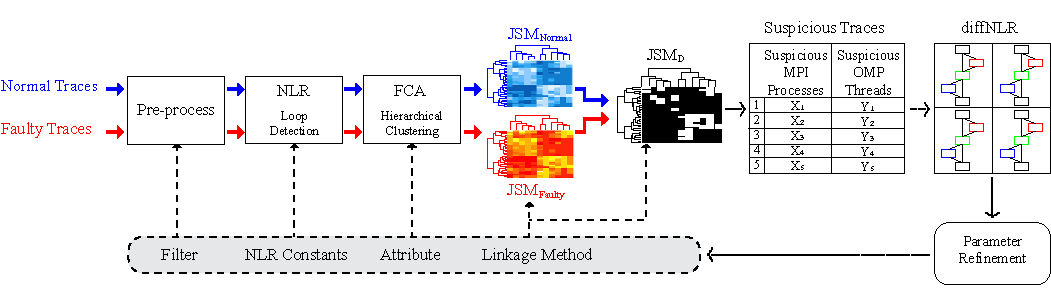
\includegraphics[width=1\textwidth]{diffTrace/figs/overview4.pdf}
%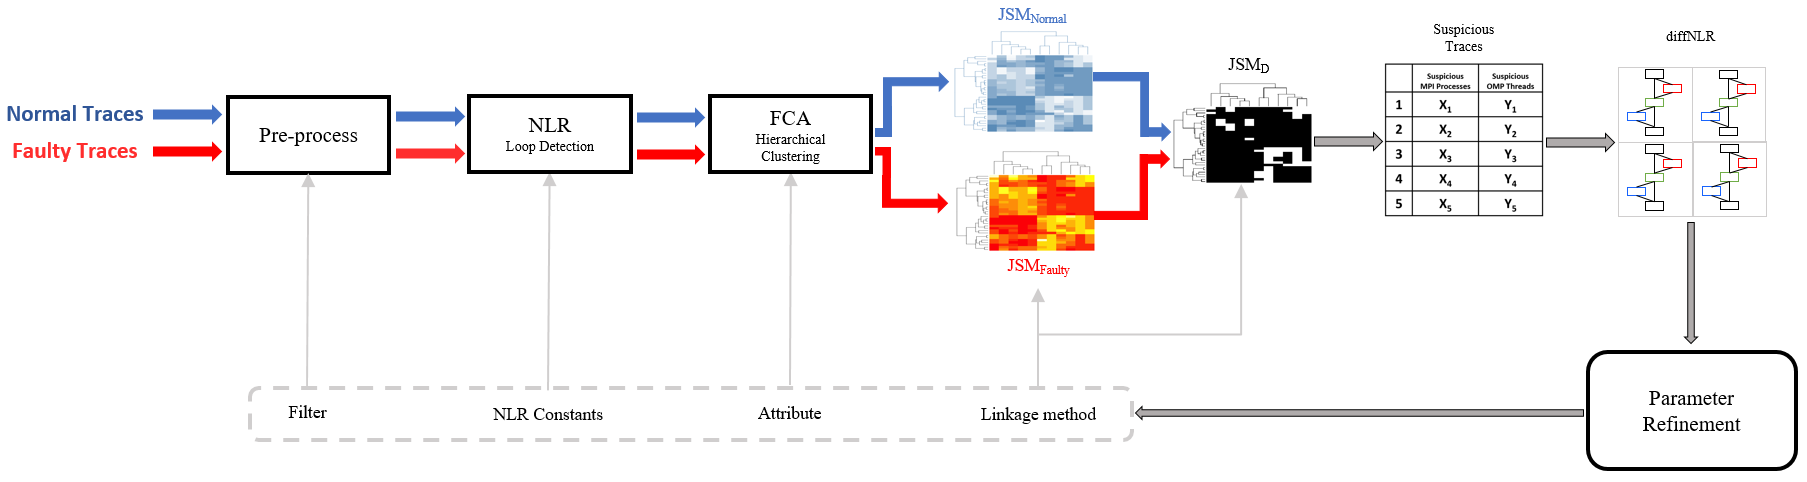
\includegraphics[]{figs/overview.png}
%\includegraphics[]{figs/overv}
\label{fig.diffTraceOverview}
\end{figure}

DiffTrace employs ParLOT's whole-program function-call and return trace-collection mechanism, where ParLOT captures traces via Pin~\cite{pin} and incrementally compresses them using a new compression scheme~\cite{parlot}.
%
ParLOT can capture functions at two levels:
the \textit{main image} (which does not include library code)
and \textit{all images} (including all library code).
%
As the application runs,
ParLOT generates per-thread trace files that
contain the compressed sequence of the IDs of the executed functions.
%
The compression mechanism is light-weight yet effective,
thus reducing not only the required bandwidth and storage but also the
runtime relative to not compressing the traces.
As a result, ParLOT can capture whole-program traces at low overhead
while leaving most of the disk bandwidth to the application.
%
Using whole-program traces substantially reduces the number of overall
debug iterations because it allows us to repeatedly analyze the
traces offline with different filters.


Figure \ref{fig.diffTraceOverview} provides an overview
of the DiffTrace toolchain
in terms of the blue flows (fault-free) and red flows
(faulty).
%
In a broad sense,
code-level faults in HPC applications (e.g.,
the use of wrong subscripts) turn into observable code-level
misbehaviors
(e.g., an unexpected number of loop iterations), many of which
turn into application-level issues.
%
In our study of DiffTrace, we evaluate
success merely in terms of the efficacy of observing
these misbehaviors in response to injected code-level
faults (we rely on a rudimentary fault injection framework
complemented by manual fault injection).

The preprocessing stage removes calls/returns at the ignored APIs.
%
The nested loop recognition (NLR)
mechanism then extracts loops from traces.
The resulting information not only
serves as a lossless abstraction to
ease the rest of the trace analysis but also
serves as a {\em per-thread measure of progress}.
%
The FCA (Formal Concept Analysis) stage conducts a systematic way to arrange objects (in our case threads)
and attributes (we support a rich collection of attributes
including the set of function calls a thread makes, the
set of {\em pairs} of function calls made---this reflects calling
context---etc.).
%
Weber et al.'s work~\cite{weberStructural,clbook} employs FCA exactly in
this manner (including the use of pairs of calls),
however, for grouping performance information.
%
Our new contribution is showing that FCA can play a central
role in debugging HPC applications.


While faults induce asymmetries (``aberrations'') in program behaviors,
one cannot locate faults merely by locating the asymmetries in
an overall collection of process traces.
%
The reason is that even in a collection of MPI processes or threads within
these processes, some processes/threads may serve as a master while others
serve as workers.
%
Thus, we must have a base level of similarities computed even for normal
behaviors and then compute how {\em this similarity relation changes} when
faults are introduced.
%
This is highlighted by
the blue and red rectangular patches in
Figure~\ref{fig.diffTraceOverview} that, respectively,
iconify the {\em Jaccard similarity
  matrices} computed for the normal behavior (above) and
the erroneous behavior (below).
%
This is shown as
the ``diff Jaccard similarity matrix'' in greyscale at the
juncture of JSM$_{normal}$ and JSM$_{faulty}$.


After the JSM$_{D}$ matrix is computed, we
invoke a hierarchical clustering algorithm that computes the ``B-score''
and helps rank suspicious traces/processes.
%
The diffNLR representation is then extracted.
%
Intuitively, this is a diff of the loop structures of the normal and abnormal
threads/processes.
%
This diagram shows (as with git diff and text diff) a {\em main stem} comprised of green rectangles
(``common looping structure'') and red/blue {\em diff rectangles} showing how the loop structures of
the normal and erroneous threads differ with respect to the main stem.
%
We show that this presentation often helps the debugging engineer
locate the faults.


Last but not least,
we strongly believe that a framework such as DiffTrace can
serve as an important HPC community resource.
%
Each debugging tool designer who uses DiffTrace can extend
it by incorporating new attributes and clustering methods, but
otherwise retain the overall tool structure.
%
Such a ``playground'' for developing and exploring new methods for
debugging does not exist in HPC.
%
There is also the intriguing possibility that
many of the 30-odd tools mentioned in \S\ref{sec:ch4_intro}
{\em can be made to focus on the problems highlighted
  by diffNLR}, thus gaining efficiency (this will be part of our future work).


In this paper, we describe DiffTrace as a
{\em relative debugging}~\cite{relative-debugging}
tool, in that bugs are caught with respect
to JSM$_{D}$ which is a {\em change} from
the previous code version found working.
%
However, many types of faults may be apparent
just by analyzing JSM$_{faulty}$: for instance,
processes whose execution got truncated
will look highly dissimilar to those that
terminated normally.
%
In those use cases of DiffTrace,
the B-score based ranking can then be made
on JSM$_{faulty}$ directly.

%---






\subsection{Example Walk-through}

We now employ
Figure~\ref{fig.oddEven}---a textbook MPI odd/even sorting example---to
illustrate DiffTrace.
%
Odd/even sorting is a parallel variant
of bubble sort
and operates in two alternating phases:
in the \textit{even phase}, the even processes exchange (conditionally swap)
values with their right neighbors, and in the \textit{odd phase},
the odd processes exchange values with their right neighbors.
%
%The for loop in line 4 of \texttt{oddEvenSort()} iterates over the phases of the algorithm. Based on the phase, the appropriate partner for each rank is computed by the function \texttt{findPtr()} (line 6). The odd/even ranks then exchange their chunks of data (lines 9-13) and sort, merge, and copy operations are performed on the received data (denoted by \texttt{...} in line 15 for simplicity).


\begin{figure}[b]
\centering
\caption{Simplified MPI implementation of Odd/Even Sort}
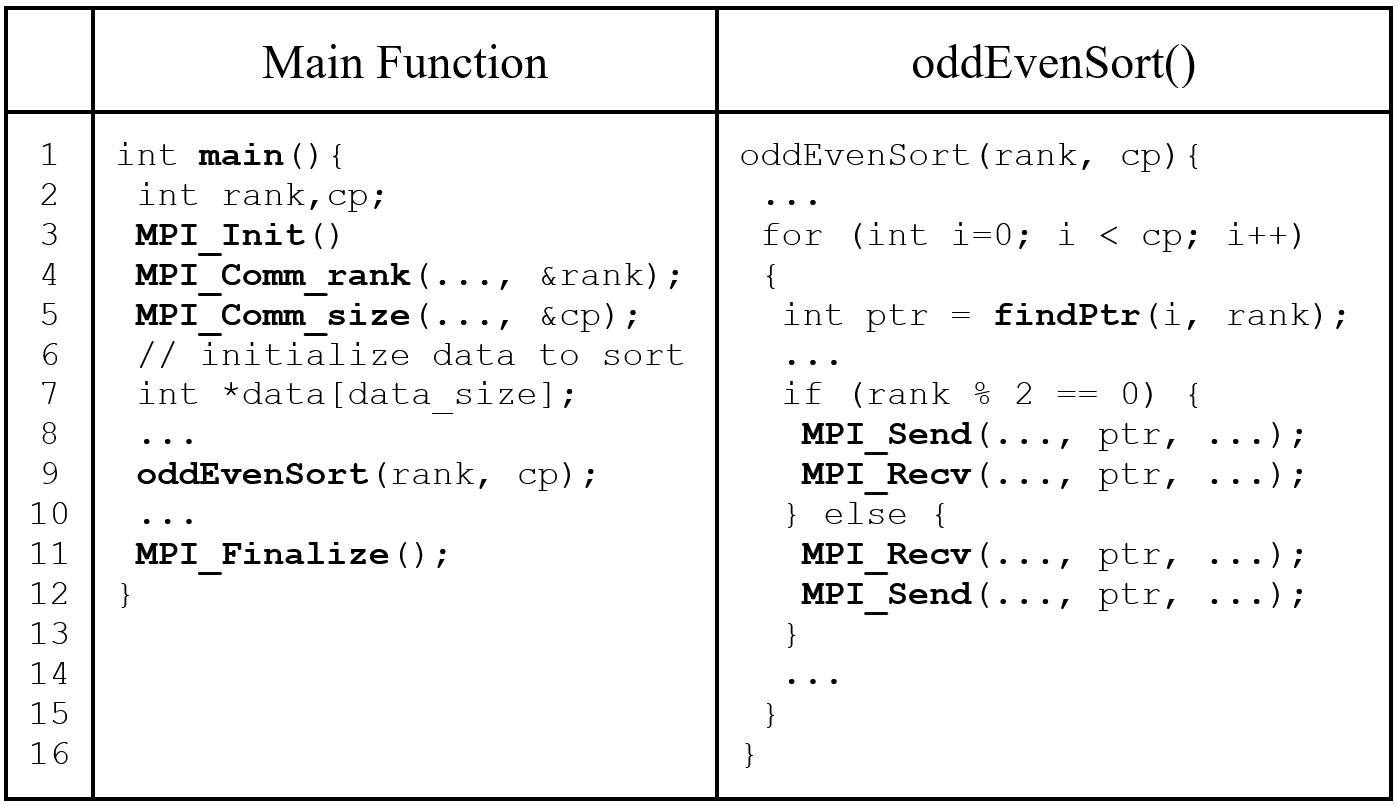
\includegraphics[width=.8\textwidth]{diffTrace/figs/oddEven.png}
\label{fig.oddEven}
\end{figure}

A waiting trap in this example is this: the user may have
swapped the {\tt Recv; Send} order in the {\tt else} part,
creating head-to-head {\tt ``Send || Send''} deadlock
under low-buffering (MPI EAGER limit).
%
We will now show how DiffTrace helps pick out this root-cause.

\subsection{Pre-processing}
% Please add the following required packages to your document preamble:
% \usepackage{multirow}
\begin{table}[]
\centering
\caption{Predefined filters}
\label{tab:filters}
\scalebox{0.72}{
\begin{tabular}{|c|c|l|}
\hline
\textbf{Category} & \textbf{Sub-Category} & \multicolumn{1}{c|}{\textbf{Description}} \\ \hline
\multirow{2}{*}{Primary} & Returns & Filter out all returns \\ \cline{2-3}
 & PLT & \begin{tabular}[c]{@{}l@{}}Filter out the ".plt" function calls for external functions/procedures that \\ their address needs to be resolved dynamically from Procedure Linkage \\ Table (PLT)\end{tabular} \\ \hline
\multirow{4}{*}{MPI} & MPI All & Only keep functions that start with "MPI\_" \\ \cline{2-3}
 & MPI Collectives & Only keep MPI collective calls (MPI\_Barrier, MPI\_Allreduce, etc) \\ \cline{2-3}
 & MPI Send/Recv & Only keep MPI\_Send, MPI\_Isend, MPI\_Recv, MPI\_Irecv and MPI\_Wait \\ \cline{2-3}
 & MPI Internal Library & Keep all inner MPI library calls \\ \hline
\multirow{3}{*}{OMP} & OMP All & Only keep OMP calls (starting with GOMP\_) \\ \cline{2-3}
 & OMP Critical & Only keep OMP\_CRITICAL\_START and OMP\_CRITICAL\_END \\ \cline{2-3}
 & OMP Mutex & Only keep OMP\_Mutex calls \\ \hline
\multirow{4}{*}{System} & Memory & Keep any memory related functions (memcpy, memchk, alloc, malloc, etc) \\ \cline{2-3}
 & Network & Keep any network related functions (network, tcp, sched, etc) \\ \cline{2-3}
 & Poll & Keep any poll related functions (poll, yield, sched, etc) \\ \cline{2-3}
 & String & Keep any string related functions (strlen, strcpy, etc) \\ \hline
\multirow{2}{*}{Advanced} & Custom & Any regular expression can be captured \\ \cline{2-3}
 & Everything & Does not filter anything \\ \hline
\end{tabular}}
\end{table}

Using ParLOT's decoder, each trace is first decompressed.
Next, the desired functions are extracted based on predefined
(Table \ref{tab:filters}) or custom regular expressions
(i.e., \textit{filters}) and kept for later phases.
%All other trace information is discarded.
%
Table \ref{tab:oddEvenPT} shows the pre-processed traces ($T_i$) of odd/even sort with four processes.
$T_i$ is the trace that stores the function calls of process $i$.

\begin{table}[]
\centering
\caption{The generated traces for odd/even execution with four processes}
\label{tab:oddEvenPT}
\scalebox{0.75}{
\begin{tabular}{|l|l|l|l|}
\hline
\rowcolor[HTML]{EFEFEF}
\multicolumn{1}{|c|}{\cellcolor[HTML]{EFEFEF}\textbf{$T_0$}} & \multicolumn{1}{c|}{\cellcolor[HTML]{EFEFEF}\textbf{$T_1$}} & \multicolumn{1}{c|}{\cellcolor[HTML]{EFEFEF}\textbf{$T_2$}} & \multicolumn{1}{c|}{\cellcolor[HTML]{EFEFEF}\textbf{$T_3$}} \\ \hline
... & ... & ... & ... \\ \\[-1em]  \hline
main & main & main & main \\ \\[-1em]  \hline
MPI\_Init & MPI\_Init & MPI\_Init & MPI\_Init \\ \\[-1em]  \hline
MPI\_Comm\_Rank & MPI\_Comm\_Rank & MPI\_Comm\_Rank & MPI\_Comm\_Rank \\ \\[-1em]  \hline
MPI\_Comm\_Size & MPI\_Comm\_Size & MPI\_Comm\_Size & MPI\_Comm\_Size \\ \\[-1em]  \hline
... & ... & ... & ... \\ \\[-1em]  \hline
oddEvenSort & oddEvenSort & oddEvenSort & oddEvenSort \\ \\[-1em]  \hline
... & ... & ... & ... \\ \\[-1em] \hline
findPtr & findPtr & findPtr & findPtr \\ \hline
\rowcolor[HTML]{FFCCC9}
{\color[HTML]{333333} MPI\_Send} & \cellcolor[HTML]{CBCEFB}{\color[HTML]{333333} MPI\_Recv} & {\color[HTML]{333333} MPI\_Send} & \cellcolor[HTML]{CBCEFB}{\color[HTML]{333333} MPI\_Recv} \\ \hline
\rowcolor[HTML]{FFCCC9}
{\color[HTML]{333333} MPI\_Recv} & \cellcolor[HTML]{CBCEFB}{\color[HTML]{333333} MPI\_Send} & {\color[HTML]{333333} MPI\_Recv} & \cellcolor[HTML]{CBCEFB}{\color[HTML]{333333} MPI\_Send} \\ \hline
... & ... & ... & ... \\ \hline
findPtr & findPtr & findPtr & findPtr \\ \hline
\rowcolor[HTML]{FFCCC9}
{\color[HTML]{333333} MPI\_Send} & \cellcolor[HTML]{CBCEFB}{\color[HTML]{333333} MPI\_Recv} & {\color[HTML]{333333} MPI\_Send} & \cellcolor[HTML]{CBCEFB}{\color[HTML]{333333} MPI\_Recv} \\ \hline
\rowcolor[HTML]{FFCCC9}
{\color[HTML]{333333} MPI\_Recv} & \cellcolor[HTML]{CBCEFB}{\color[HTML]{333333} MPI\_Send} & {\color[HTML]{333333} MPI\_Recv} & \cellcolor[HTML]{CBCEFB}{\color[HTML]{333333} MPI\_Send} \\ \hline
... & ... & ... & ... \\ \hline
MPI\_Finalize & MPI\_Finalize & MPI\_Finalize & MPI\_Finalize \\ \hline
\end{tabular}}
\end{table}






\subsection{Nested Loop Representation}

Virtually all dynamic statements are found within loops.
%
Function calls within a loop body yield \textit{repetitive patterns}
in ParLOT traces.
%
Inspired by ideas for the detection of repetitive patterns in strings \cite{nakamura_fast_2013}
and other data structures \cite{kmr},
we have adapted the Nested Loop Recognition (NLR) algorithm by Ketterlin et al.~\cite{Ketterlin-nlr}
to detect repetitive patterns in ParLOT traces (cf.~Section \ref{subsec:algo-nlr}).
Detecting such patterns can be used to measure the progress of each thread,
revealing unfinished or broken loops that may be the consequence of a fault.



\begin{table}[]
\centering
\caption{NLR of traces}
\label{tab:oddEvenPT-NLR}
\scalebox{0.75}{
\begin{tabular}{|l|l|l|l|}
\hline
\rowcolor[HTML]{EFEFEF}
\multicolumn{1}{|c|}{\cellcolor[HTML]{EFEFEF}\textbf{$T_0$}} & \multicolumn{1}{c|}{\cellcolor[HTML]{EFEFEF}\textbf{$T_1$}} & \multicolumn{1}{c|}{\cellcolor[HTML]{EFEFEF}\textbf{$T_2$}} & \multicolumn{1}{c|}{\cellcolor[HTML]{EFEFEF}\textbf{$T_3$}} \\ \hline
MPI\_Init & MPI\_Init & MPI\_Init & MPI\_Init \\ \\[-1em]  \hline
MPI\_Comm\_Rank & MPI\_Comm\_Rank & MPI\_Comm\_Rank & MPI\_Comm\_Rank \\ \\[-1em]  \hline
MPI\_Comm\_Size & MPI\_Comm\_Size & MPI\_Comm\_Size & MPI\_Comm\_Size \\ \\[-1em]  \hline
\rowcolor[HTML]{FFCCC9}
{\color[HTML]{333333} L0 \^{} 2} & \cellcolor[HTML]{CBCEFB}{\color[HTML]{333333} L1 \^{} 4} & {\color[HTML]{333333} L0 \^{} 4} & \cellcolor[HTML]{CBCEFB}{\color[HTML]{333333} L1 \^{} 2} \\ \hline
MPI\_Finalize & MPI\_Finalize & MPI\_Finalize & MPI\_Finalize \\ \hline
\end{tabular}}
\end{table}



For example, the loop in line 3 of \texttt{oddEvenSort()} (Figure \ref{fig.oddEven}) iterates
four times when run with four processes.
Thus each $T_i$ contains four occurrences of either [\texttt{MPI\_Send}-\texttt{MPI\_Recv}] (even $i$)
or [\texttt{MPI\_Recv}-\texttt{MPI\_Send}] (odd $i$).
By keeping only MPI functions and converting each $T_i$ into its equivalent NLR,
Table \ref{tab:oddEvenPT} can be reduced to Table \ref{tab:oddEvenPT-NLR} where \textbf{L0} and \textbf{L1}
represent the \textit{loop body} [\texttt{MPI\_Send}-\texttt{MPI\_Recv}] and
[\texttt{MPI\_Recv}-\texttt{MPI\_Send}], respectively.
The integer after the \^{} symbol in NLR represents the \textit{loop iteration count}.
Note that, since the first and last processes only have one-way communication with their neighbors,
$T_0$ and $T_3$ perform only half as many iterations.

\begin{table}[]
\caption{Formal Context of odd/even sort example}
\label{tab:sampleContext}
\scalebox{0.7}{
\begin{tabular}{l|cccccc}
 & \multicolumn{1}{l}{MPI\_Init()} & \multicolumn{1}{l}{MPI\_Comm\_Size()} & \multicolumn{1}{l}{MPI\_Comm\_Rank()} & \multicolumn{1}{l}{L0} & \multicolumn{1}{l}{L1} & \multicolumn{1}{l}{MPI\_Finalize()} \\ \hline
Trace 0 & $\times$ & $\times$ & $\times$ & $\times$ &  & $\times$ \\
Trace 1 & $\times$ & $\times$ & $\times$ &  & $\times$ & $\times$ \\
Trace 2 & $\times$ & $\times$ & $\times$ & $\times$ &  & $\times$ \\
Trace 3 & $\times$ & $\times$ & $\times$ &  & $\times$ & $\times$
\end{tabular}}
\end{table}

\subsection{Hierarchical Clustering via FCA}
Processes in HPC applications are known to fall into predictable equivalence classes.
%
The widely used and highly successful STAT tool~\cite{stat} owes most of its
success for being able to efficiently collect stack traces (nested sequences of function
calls), organize them as prefix-trees, and equivalence the processes into teams that
evolve in different ways.
%
Coalesced stack trace graphs (CSTG, \cite{cstg}) have proven effective in
locating bugs within Uintah~\cite{uintah} and perform stat-like equivalence class formation,
albeit with the added detail of maintaining calling contexts.
%
Inspired by these ideas, FCA-based clustering provides the next logical level of refinement
in the sense that (1)~we can pick any of the multiple attributes one can mine from traces (e.g.,
pairs of function calls, memory regions accessed by processes, locks held by threads, etc.), and (2)~form this equivalencing relation quite naturally by computing the Jaccard distance between processes/threads.
%
In general,
such a classification is powerful enough to
distinguish structurally different threads from one another
(e.g., MPI processes from OpenMP threads in hybrid MPI+OpenMP applications)
and reduce the search space for bug location to a few representative classes of traces that
are distinctly dissimilar.\footnote{As emphasized earlier, we perform ``sky subtraction'' as
  in astronomy to locate comets; in our case, we diff the diffs, which is
  captured in JSM$_{D}$.}

A \textit{formal context} is a triple $K = (G, M, I)$
where $G$ is a set of \textbf{objects},
$M$ is a set of \textbf{attributes},
and $I \subseteq G \times M$ is an incidence relation that expresses
\textit{which objects have which attributes}.
Table \ref{tab:sampleContext} shows the formal context of the preprocessed odd/even-sort traces.
%
We can employ as attributes either the function calls themselves or the detected loop bodies
(each detected loop is assigned a unique ID, and one can diff with respect to these IDs).
%
The context shows that all traces include the functions MPI\_Init(),
MPI\_Comm\_size(), MPI\_Comm\_rank() and MPI\_Finalize().
The even traces contain the loop \textit{L0} and the odd traces the loop \textit{L1}.
%

% \hl{Definition of formal concept (needed?) figure }\ref{fig:formalConceptDefinition} :
%
% \begin{figure}[]
% \centering
% \caption{Formal Concept Definition}
% 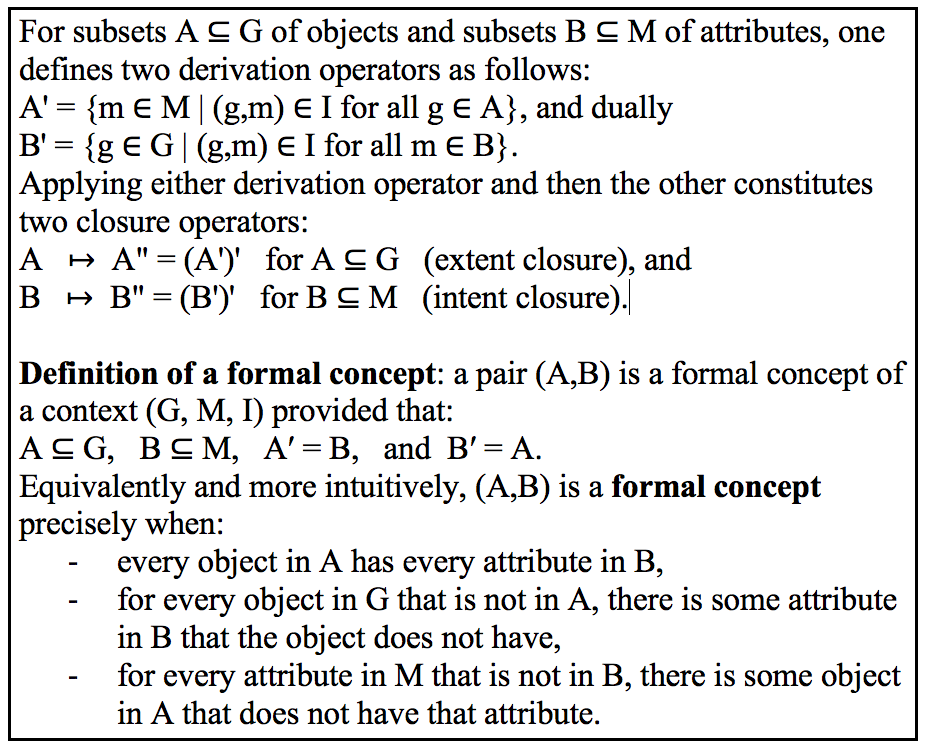
\includegraphics[width=0.45\textwidth]{figs/formalConceptDefinition.png}
% \label{fig:formalConceptDefinition}
% \end{figure}

%A \textit{concept lattice} can be derived from a \textit{formal context} by specifying \textit{formal concepts}
%(Figure \ref{fig:formalConceptDefinition})
%and a \textit{partial order} on them.
%Concept lattices are represented as a directed acyclic graph where concepts are nodes and the
%order on them determines the edges.
%
Figure \ref{fig:sampleCL} shows the concept lattice derived from the formal context in
Table~\ref{tab:sampleContext} and is interpreted as follows:

\begin{compactitem}
\item The top node indicates that all traces share MPI\_Init(),
  MPI\_Comm\_size(), MPI\_Comm\_rank() and MPI\_Finalize().
    \item The bottom node signifies that none of the traces share all attributes.
    \item The middle nodes show that $T_0$ and $T_2$ are different from  $T_1$ and $T_3$.
\end{compactitem}



% Once the redundant labels are removed from the lattice, each object (trace) and attribute appears in the lattice exactly once. Consequently, the nodes of the lattice form the desired grouping, since it is guaranteed that each trace belongs to exactly one group. However, the concept lattice itself does not provide similarity values for the distinct groups of traces. The \textit{Jaccard Index}, also known as \textit{Intersection over Union}, measures the \textit{distance} between sets $A$ and $B$ in terms of the ratio of the \textit{intersection} size of $A$ and $B$ over the size of their \textit{union}.
%

%


\begin{figure}[t]
\centering
\begin{minipage}{.45\textwidth}
  \centering
  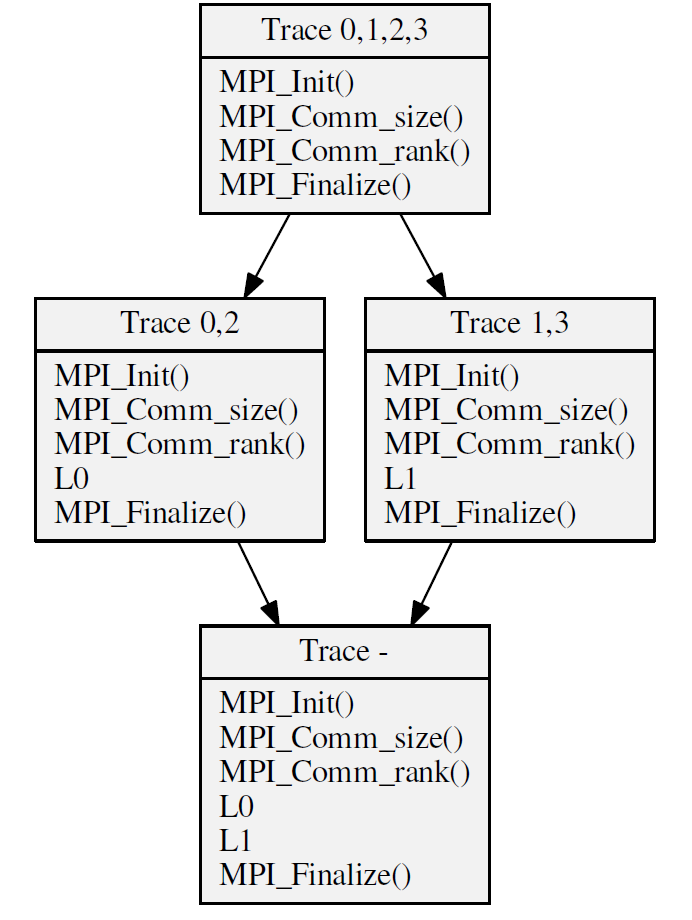
\includegraphics[width=.9\linewidth]{diffTrace/figs/sampleCL.png}
  \caption{Sample Concept Lattice from Object-Attribute Context in Table \ref{tab:sampleContext}}
  \label{fig:sampleCL}
\end{minipage}
\begin{minipage}{.45\textwidth}
\centering
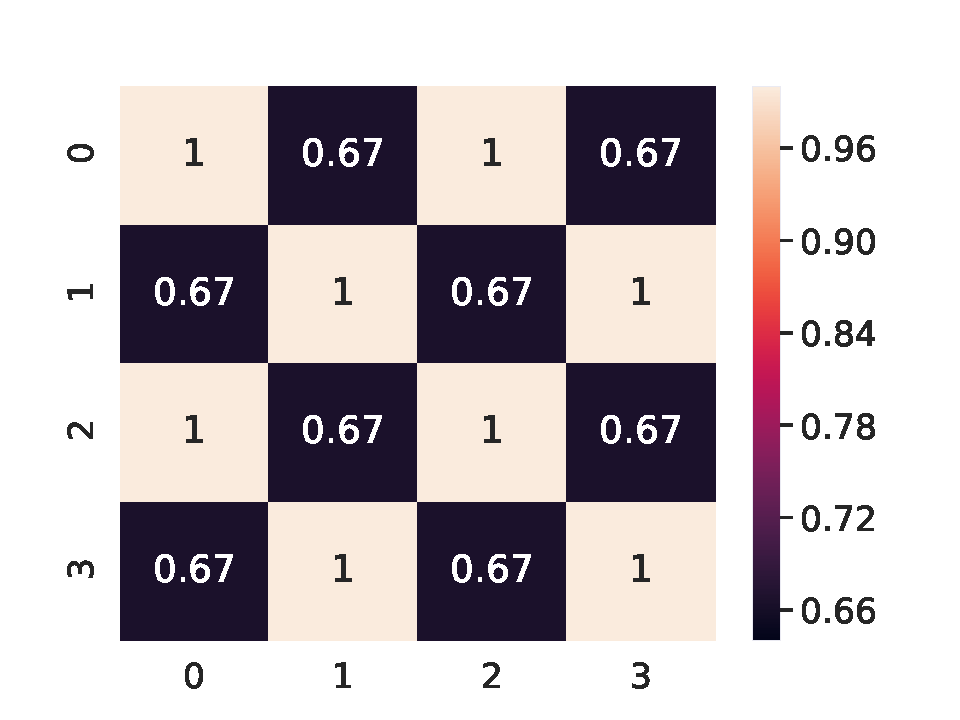
\includegraphics[width=.9\linewidth]{diffTrace/figs/oddEvenJSM2.pdf}
\caption{Pairwise Jaccard Similarity Matrix (JSM) of MPI Processes in Sample Code}
\label{fig:jsm2}
\end{minipage}

\end{figure}


%\begin{figure}[]
%\centering
%\scalebox{0.8}{
%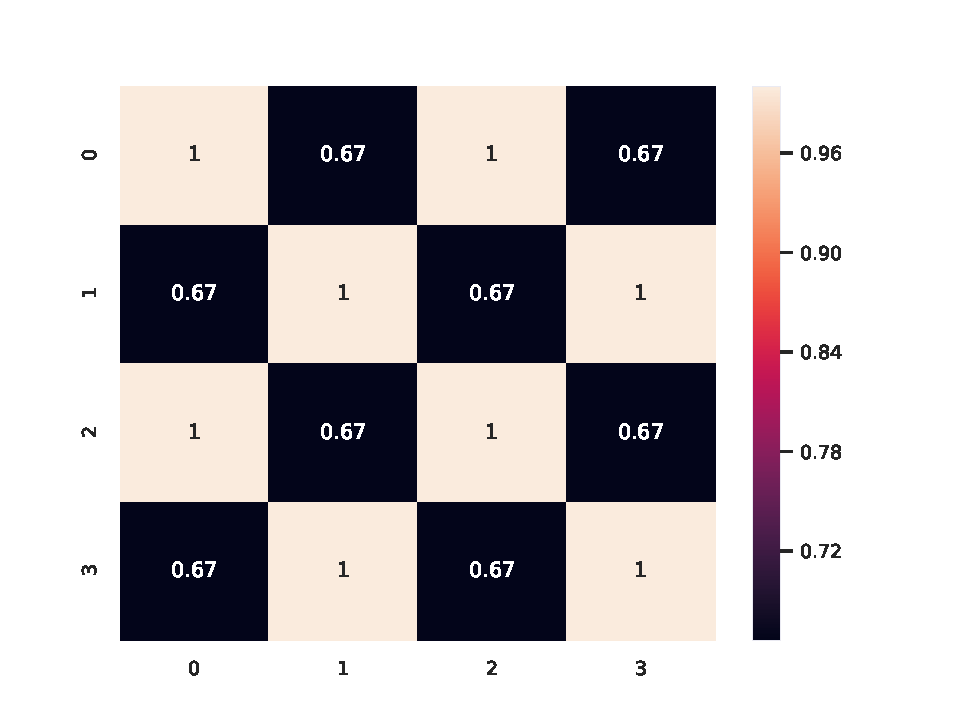
\includegraphics[width=3.4in]{figs/oddEvenJSM.pdf}}
%\caption{Pairwise Jaccard Similarity Matrix (JSM) of MPI processes in sample code}
%\label{fig:jsm}
%\end{figure}


% For any pair of $(T_i, T_j)$, the number of attributes in the Lowest Common Ancestor (LCA) node of $T_i$ and $T_j$ in the lattice is the number of attributes that $T_i$ and $T_j$ have in common (intersection). The sum of the number of attributes of the nodes on the path from each $T_i$ and $T_j$ to their LCA is the union. This property is one of the motivations for using concept lattices as classifier since it makes computing the union and intersection easy and fast.
%
% Some algorithms for extracting concepts from contexts and constructing the concept lattice require the whole context to be present in the memory.
%

The complete pairwise Jaccard Similarity Matrix (JSM) can easily be computed from concept lattices.
%
For large-scale executions with thousands of threads, it is imperative
to employ incremental algorithms to
construct concept lattices (detailed in Section \ref{subsec:algo-cl}).
%
% Through an incremental concept-lattice-construction approach,
% DiffTrace extracts attributes (\hl{table that shows attributes})
% from NLR traces and injects them into a concept lattice one trace at a time
%
Figure \ref{fig:jsm2}
shows the heatmap
% (explain this)
of the JSM obtained from the concept lattice in Figure \ref{fig:sampleCL}.
%
DiffTrace uses the JSM to form equivalence classes of traces by hierarchical clustering.
%
Next, we show how the differences between two hierarchical clusterings from two executions
(faulty vs.~normal) reveal which traces have been affected the most by the fault.


\subsection{Detecting Suspicious Traces via JSM$_{D}$}
% So far,
% we have explained how DiffTrace can narrow down the search space from numerous long traces to just a few equivalent JSMs (i.e., clusters).
% %
JSM$_{normal}$[i][j] (JSM$_{faulty}$[i][j]) shows the Jaccard similarity score of $T_i$ and $T_j$ from the normal trace ($T_i^\prime$ and $T_j^\prime$).
%
% However, we are interested in detecting what changed the most due to the fault.
% with respect to the ``natural asymmetry'' of the application.
%
%In other words, DiffTrace abstracts function call traces into JSMs, which are reflections of asymmetry among traces.
As explained earlier, we compute
JSM$_{D}$ to detect outlier executions, where
JSM$_{D}$ = $|$JSM$_{faulty} - $JSM$_{normal}|$.

%
We sort the suggestion table based on the \textit{B-score}
similarity metric of two hierarchical clusterings \cite{fowlkes83} (cf.~Section \ref{subsec:algo-bscore}).
%
A single iteration through the
DiffTrace loop
(with a single set of parameters shown as a dashed box in Figure \ref{fig.diffTraceOverview})
may still not detect the root-cause of a bug.
%
The user can then (1)~alter the linkage method employed in computing the hierarchical clustering
(reorder the dendrograms built to achieve the clustering),
(2)~alter the FCA attributes, (3)~adjust the NLR constants (loops are extracted with
realistic complexity by observing repetitive patterns inside a preallocated buffer),
and/or (4)~the front-end filters.
%
This is shown in the iterative loop in
Figure \ref{fig.diffTraceOverview}.

\subsection{Evaluation}

%The resulting outlier traces are candidates for the potential cause of the change in the program behavior and thus, a potential fault root cause or fault manifestation.
%

%
%Also, a different set of parameters might produce inaccurate suggestions (false positives).
%

\begin{figure}[t]
\begin{minipage}{.2\textwidth}
\centering
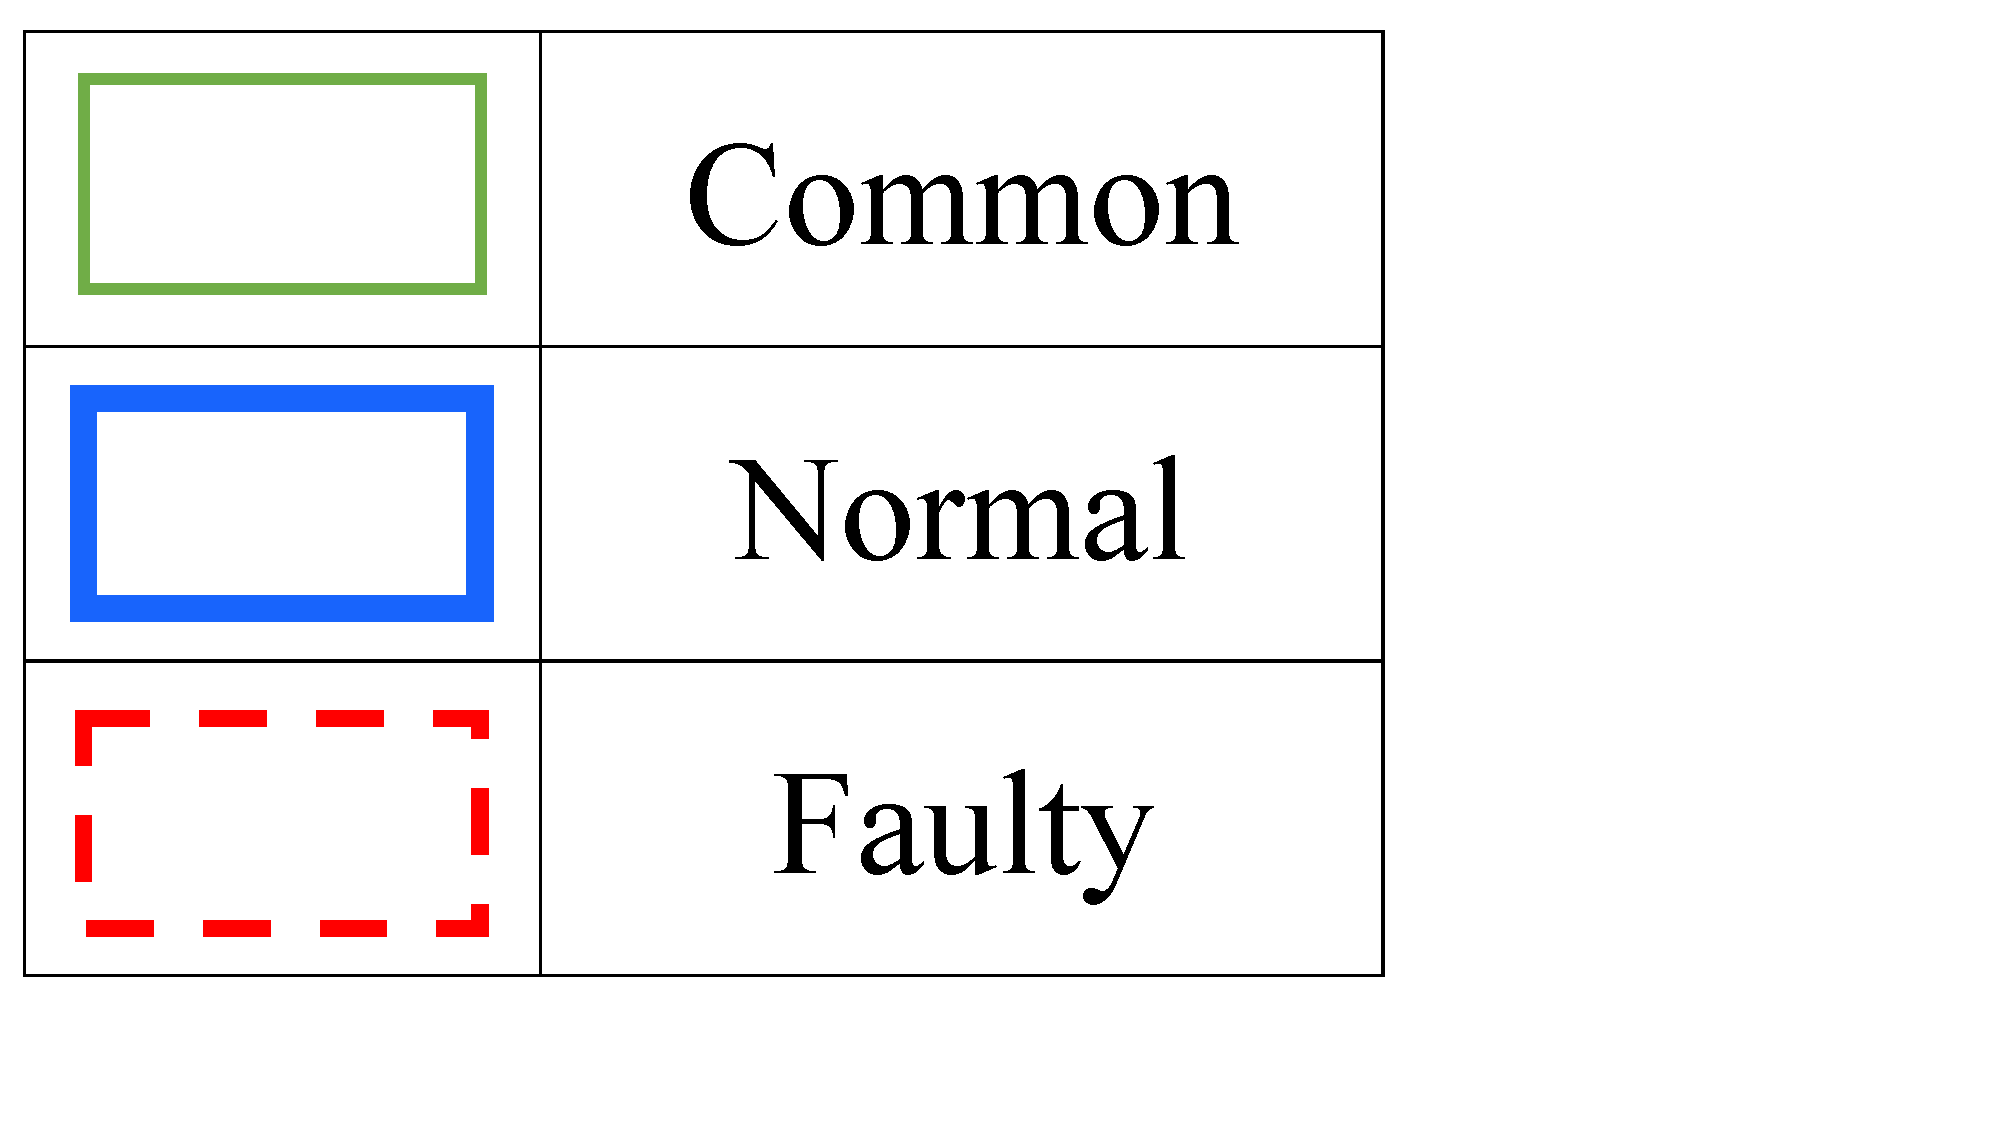
\includegraphics[width=\textwidth]{diffTrace/figs/legend.pdf}
\caption{Legend}
\label{fig:legend}
\end{minipage}
\begin{minipage}{.38\textwidth}
    \centering
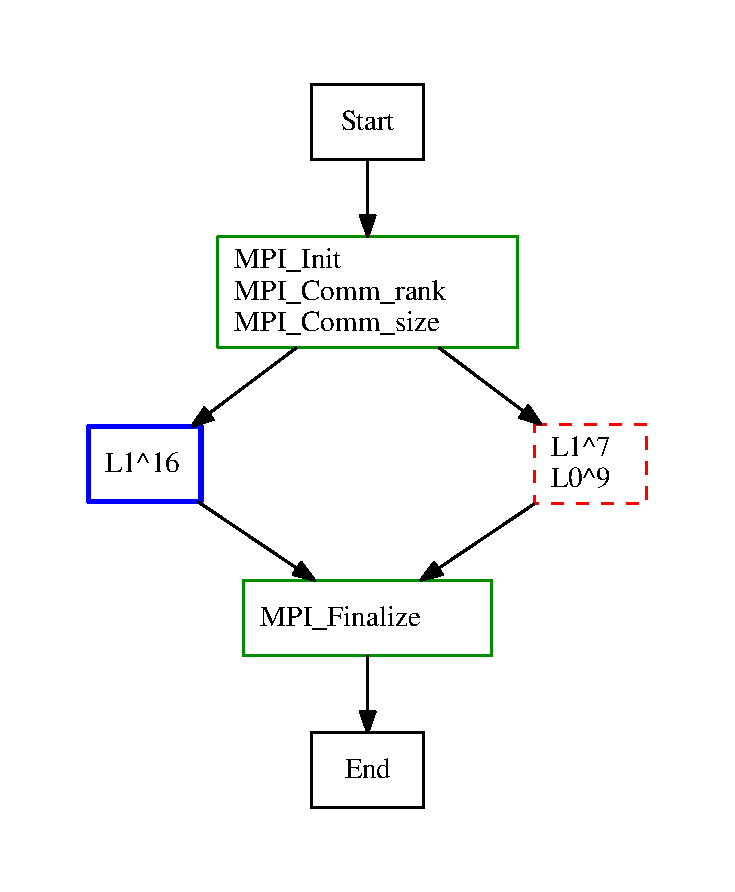
\includegraphics[width=\textwidth]{diffTrace/figs/b-11.mpi.0K10-5.pdf}
\caption{swapBug}
\label{fig:swapbug}
\end{minipage}
%\caption{diffNLR Example}
%\label{fig:sampleDiffNLR}
\begin{minipage}{.38\textwidth}
\centering
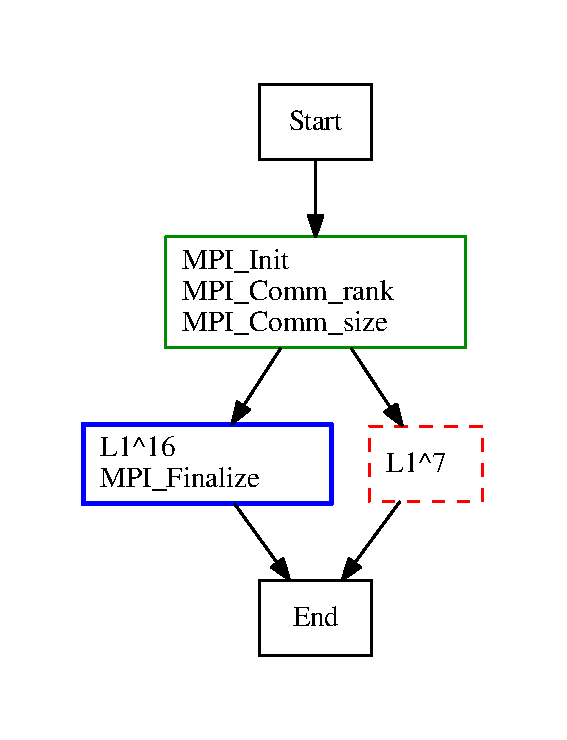
\includegraphics[width=0.9\linewidth]{diffTrace/figs/adl-11.mpi.0K10-5.pdf}
\caption{dlBug}
\label{fig:dlbug}
\end{minipage}
\end{figure}

To evaluate the effectiveness of DiffJSM, we planted two artificial bugs (\textit{swapBug}
and \textit{dlBug}) in the code from Figure \ref{fig.oddEven} and ran it with 16 processes.
%
\textit{swapBug} swaps the order of MPI\_Send and MPI\_Recv in rank 5
after the seventh iteration of the loop in line 3 of \texttt{oddEvenSort},
simulating a potential deadlock. \textit{dlBug} simulates an actual deadlock in the same location
(rank 5 after the seventh iteration).
%
Upon collection of ParLOT traces from the execution of the buggy code versions,
DiffTrace first decompresses them and filters out all non-MPI functions.
Then two major loops are detected, \textbf{L0} and \textbf{L1} (identical to the ones in Table \ref{tab:oddEvenPT-NLR}),
that are supposed to loop 16 times in the even and odd traces,
respectively (except for the first and last traces, which loop just eight times).

After constructing concept lattices and their corresponding JSMs, trace 5 appears as the trace that got
affected the most by the bugs because row 5 (showing the similarity score of $T_5$ relative to all other traces)
(JSM$_{normal}$[5][i] for $i \in [0,16)$)
  changed the most after the bug was introduced.
  %Consequently, it means that $T^\prime_5$ affected the asymmetry of all $T_i$s.
%
The differences between the suggested suspicious trace ($T^\prime_s$)
and its corresponding normal trace ($T_s$) is visualized by \textit{diffNLR}.


\subsubsection{diffNLR}
To highlight the differences in an easy-to-understand manner, DiffTrace visually separates the common and different blocks of a pair of pre-processed traces via \textit{diffNLR}, a graphical visualization of the \texttt{diff} algorithm \cite{diff-myers}.
%






\texttt{diff} takes two sequences $S_A$ and $S_B$ and computes the minimal \textit{edit} to convert $S_A$ to $S_B$. This algorithm is used in the GNU \texttt{diff} utility to compare two text files and in git for efficiently keeping track of file changes.
Since ParLOT preserves the order of function calls, each trace $T_i$ is totally ordered. Thus \textit{diff} can expose the differences of a pair of $T$s. \textit{diffNLR} aligns common and different blocks of a pair of sequences (e.g., traces) horizontally and vertically, making it easier for the analyst to see the differences at a glance.
For simplicity, our implementation of \textit{gdiff} only takes one argument $x$ that denotes \textit{the suspicious trace}.

diffNLR$(x) \equiv $ diffNLR$(T_x,T_x^\prime)$
%
where $T_x$ is the trace of thread/process $x$ of a normal execution and $T^\prime_x$ is the corresponding trace of the faulty execution.

Figure \ref{fig:swapbug} shows the diffNLR(5) of \textit{swapBug} where $T_5$ iterates over the loop [MPI\_Recv - MPI\_Send] 16 times (L1\^{}16) after the MPI initialization while the order swap is well reflected in $T_5^\prime$ (L1\^{}7 - L0\^{}9). Both processes seem to terminate fine by executing MPI\_Finalize().
However, diffNLR(5) of \textit{dlBug} (Figure \ref{fig:dlbug}) shows that, while $T_5$ executed MPI\_Finalize, $T_5^\prime$ got stuck after executing L1 seven times and never reached MPI\_Finalize.

This example illustrates how our approach can locate the part of each execution that was impacted by a fault. Having an understanding of \textit{how the application should behave normally} can reduce the number of iterations by picking the right set of parameters sooner.


%\begin{figure}[]
%\centering
%\caption{A line change in oddEvenSort (left) that might cause a deadlock in oddEvenSort\_DL (right)}
%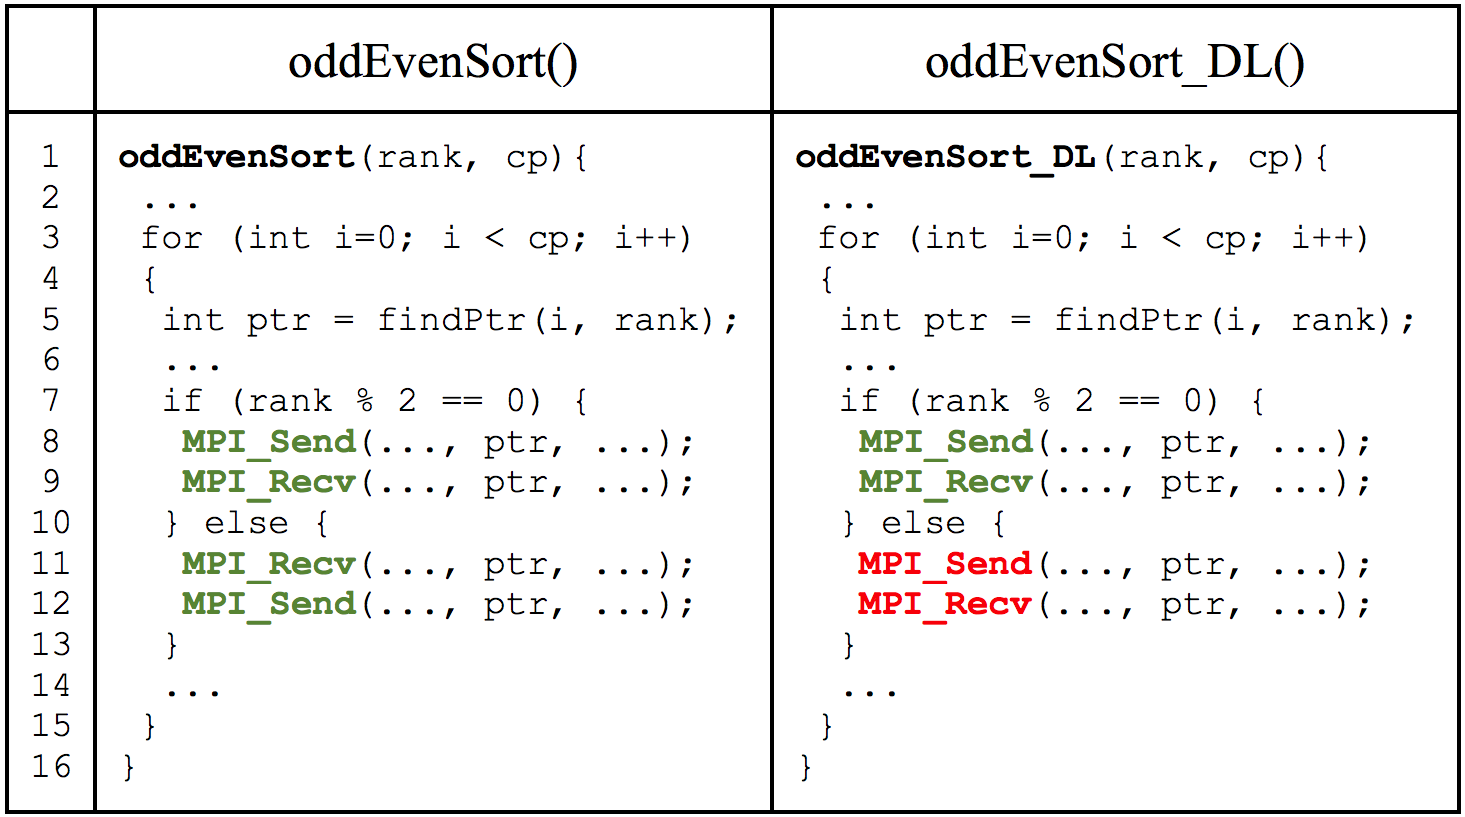
\includegraphics[width=0.45\textwidth]{figs/oddEvenDL.png}
%\label{fig.oddEvenDL}
%\end{figure}


\begin{frame}{}
  \lstset{language=C}
 \begin{lstlisting}[caption={ILCS Overview},label={lst:ilcs}]
main(argc, argv) {
 ... // initialization
 MPI_Init();
 MPI_Comm_size();
 MPI_Comm_rank(my_rank);
 ... // Obtain number of local CPUs and GPUs
 MPI_Reduce(lCPUs, gCPUs, MPI_SUM); // Total # of CPUs
 MPI_Reduce(lGPUs, gGPUs, MPI_SUM); // Total # of GPUs
 champSize = CPU_Init();
 ... // Memory allocation for storing local and global champions w.r.t. champSize
 MPI_Barrier();
 <@\textcolor{blue} {\#pragma omp parallel num\_threads(lCPUs+1)}@>
 {rank = omp_get_thread_num();
  if (rank != 0) { // worker threads
   while (cont) {
    ... // calculate seed
    local_result = CPU_Exec();
    if (local_result < champ[rank]) { // update local champion
     <@\textcolor{blue}{\#pragma omp critical}@>
     memcpy(champ[rank], local_result);}}
  } else { //master thread
   do {
    ...
    MPI_AllReduce(); //broadcast the global champion 
	  ...
    MPI_AllReduce(); //broadcast the global champion P_id
    ...
    if (my_rank == global_champion_P_id) {
     <@\textcolor{blue}{\#pragma omp critical}@>
     memcpy(bcast_buffer, champ[rank]);
    }
    MPI_Bcast(bcast_buffer); // broadcast the local champion to all nodes
   } while (no_change_threshold);
   cont = 0; // signal worker threads to terminate
  }}
 if (my_rank == 0) {CPU_Output(champ);}
 MPI_Finalize();}

/* User code for TSP problem */
CPU_Init() {/* Read coordinates, calculate distances, initialize champion structure, return structure size */}
CPU_Exec() {/* Find local champions (TSP tours) */}
CPU_Output() {/* Output champion */}
\end{lstlisting}
\end{frame}

\begin{table}[t]
\centering
\caption{Ranking table - OpenMP bug: unprotected shared memory access by thread 4 of process 6}
\label{tab:mc1-mc-6-4}
\scalebox{0.78}{
\begin{tabular}{|c|c|c|c|c|}
\hline
 Filter                           & Attributes   &   B-score & \begin{tabular}[c]{@{}c@{}}Top\\Processes\end{tabular}          & \begin{tabular}[c]{@{}c@{}}Top\\Threads\end{tabular}  \\
\hline
 11.plt.mem.cust.0K10             & doub.noFreq  &     0.244 & 7, 3, 4         & \textbf{6.4}, 7.3, 1.4, 3.3, 3.4, 4.2  \\
 11.plt.mem.cust.0K10             & doub.log10   &     0.244 & 7, 3, 4         & \textbf{6.4}, 7.3, 1.4, 3.3, 3.4, 4.2  \\
 01.plt.mem.cust.0K10             & doub.noFreq  &     0.244 & 7, 3, 4         & \textbf{6.4}, 7.3, 1.4, 3.3, 3.4, 4.2  \\
 01.plt.mem.cust.0K10             & doub.log10   &     0.244 & 7, 3, 4         & \textbf{6.4}, 7.3, 1.4, 3.3, 3.4, 4.2  \\
 01.mem.ompcrit.cust.0K10         & sing.log10   &     0.262 & 3                 & \textbf{6.4}, 7.1, 3.3, 4.1, 5.1, 6.1  \\
 01.mem.ompcrit.cust.0K10         & sing.noFreq  &     0.262 & 3                 & \textbf{6.4}, 7.1, 3.3, 4.1, 5.1, 6.1  \\
 11.mem.ompcrit.cust.0K10         & sing.log10   &     0.262 & 3                 & \textbf{6.4}, 7.1, 3.3, 4.1, 5.1, 6.1  \\
 11.mem.ompcrit.cust.0K10         & sing.noFreq  &     0.262 & 3                 & \textbf{6.4}, 7.1, 3.3, 4.1, 5.1, 6.1  \\
% 01.plt.mem.mpi.ompall.cust.0K10  & sing.actual  &     0.266 &                    & 2.4 , 4.3 ,                         \\
% 11.plt.mem.mpi.ompall.cust.0K10  & sing.actual  &     0.266 &                    & 2.4 , 4.3 ,                         \\
 11.plt.mem.cust.0K10             & doub.actual  &     0.273 & 7                 & \textbf{6.4}, 2.4, 3.4, 4.2, 4.4        \\
 01.plt.mem.cust.0K10             & doub.actual  &     0.273 & 7                 & \textbf{6.4}, 2.4, 3.4, 4.2, 4.4        \\
% 11.plt.mem.mpi.ompcrit.cust.0K10 & doub.noFreq  &     0.276 & 3 ,                & 3.3 , \textbf{6.4} ,                         \\
% 11.plt.mem.mpi.ompcrit.cust.0K10 & doub.log10   &     0.276 & 3 ,                & 3.3 , \textbf{6.4} ,                         \\
% 01.plt.mem.mpi.ompcrit.cust.0K10 & doub.noFreq  &     0.276 & 3 ,                & 3.3 , \textbf{6.4} ,                         \\
% 01.plt.mem.mpi.ompcrit.cust.0K10 & doub.log10   &     0.276 & 3 ,                & 3.3 , \textbf{6.4} ,                         \\
\hline
\end{tabular}}
\end{table}


\begin{table}[b]
\centering
\caption{Ranking table - MPI bug: wrong collective size in process 2}
\label{tab:ar1-ws-all-nn}
\scalebox{0.81}{
\begin{tabular}{|c|c|c|c|c|}
\hline
 Filter              & Attributes   &    B-score & \begin{tabular}[c]{@{}c@{}}Top\\Processes\end{tabular}          & \begin{tabular}[c]{@{}c@{}}Top\\Threads\end{tabular}         \\
\hline
% 11.mem.mpicol.ompcrit.cust.0K10 & sing.log10   &      0.383 & 0 , 7 , 2 , 4 , 5 , 6 , & 1.1 , 1.3 , 1.4 , 3.1 , 3.2 , 3.4 , \\
% 11.mem.mpicol.ompcrit.cust.0K10 & sing.noFreq  &      0.383 & 0 , 7 , 2 , 4 , 5 , 6 , & 1.1 , 1.3 , 1.4 , 3.1 , 3.2 , 3.4 , \\
 11.mpicol.cust.0K10             & sing.log10   &      0.439 & 0, 7, 2, 4, 5, 6  & 1.1, 1.3, 3.1, 3.2, 3.4        \\
 11.mpicol.cust.0K10             & sing.noFreq  &      0.439 & 0, 7, 2, 4, 5, 6  & 1.1, 1.3, 3.1, 3.2, 3.4        \\
 11.mpi.cust.0K10                & doub.noFreq  &      0.457 & 0, 7, 2, 4, 5, 6  & 1.4, 3.3, 3.4                    \\
 11.mpi.cust.0K10                & doub.actual  &      0.457 & 0, 7, 2, 4, 5, 6  & 1.4, 3.3, 3.4                    \\
 11.mpiall.cust.0K10             & doub.noFreq  &      0.457 & 0, 7, 2, 4, 5, 6  & 1.4, 3.3, 3.4                    \\
 11.mpiall.cust.0K10             & doub.actual  &      0.457 & 0, 7, 2, 4, 5, 6  & 1.4, 3.3, 3.4                    \\
 11.mpicol.cust.0K10             & doub.noFreq  &      0.457 & 0, 7, 2, 4, 5, 6  & 1.4, 3.3, 3.4                    \\
 11.mpicol.cust.0K10             & doub.actual  &      0.457 & 0, 7, 2, 4, 5, 6  & 1.4, 3.3, 3.4                    \\
 11.mpi.cust.0K10                & sing.log10   &      0.465 & 0, 7, 2, 4, 5, 6  & 1.1, 1.3, 3.1, 3.2, 3.4        \\
 11.mpi.cust.0K10                & sing.noFreq  &      0.465 & 0, 7, 2, 4, 5, 6  & 1.1, 1.3, 3.1, 3.2, 3.4        \\
 11.mpiall.cust.0K10             & sing.log10   &      0.465 & 0, 7, 2, 4, 5, 6  & 1.1, 1.3, 3.1, 3.2, 3.4        \\
 11.mpiall.cust.0K10             & sing.noFreq  &      0.465 & 0, 7, 2, 4, 5, 6  & 1.1, 1.3, 3.1, 3.2, 3.4        \\
 11.mpi.cust.0K10                & doub.noFreq  &      0.543 & 0, 7, 2, 4, 5, 6  & 1.4, 3.3, 3.4                    \\
 11.mpi.cust.0K10                & doub.actual  &      0.543 & 0, 7, 2, 4, 5, 6  & 1.4, 3.3, 3.4                    \\
\hline
\end{tabular}}
\end{table}

\begin{table}[b]
\centering
\caption{Ranking Table - MPI-Bug: Wrong Collective Operation ,Injected to Process 0}
\label{tab:ar1-wo-0-nn}
\scalebox{0.81}{
\begin{tabular}{|c|c|c|c|c|}
\hline
 Filter              & Attributes   &    B-score & \begin{tabular}[c]{@{}c@{}}Top\\Processes\end{tabular}          & \begin{tabular}[c]{@{}c@{}}Top\\Threads\end{tabular}  \\
\hline
 01.plt.cust.0K10    & doub.log10   &      0.271 & 2                 & 6.2, 7.3, 2.2, 5.2, 5.3  \\
 11.plt.cust.0K10    & doub.log10   &      0.271 & 2                 & 6.2, 7.3, 2.2, 5.2, 5.3  \\
 01.plt.cust.0K10    & sing.actual  &      0.276 & 1                 & 3.1, 1.4, 6.4, 3.4        \\
 11.plt.cust.0K10    & sing.actual  &      0.276 & 1                 & 3.1, 1.4, 6.4, 3.4        \\
 01.plt.cust.0K10    & doub.noFreq  &      0.285 & 2                 & 6.2, 7.3, 2.2, 5.2, 5.3  \\
 11.plt.cust.0K10    & doub.noFreq  &      0.285 & 2                 & 6.2, 7.3, 2.2, 5.2, 5.3  \\
 01.plt.cust.0K10    & sing.log10   &      0.292 & 1, 4, 5  & 3.1, 4.3                    \\
 11.plt.cust.0K10    & sing.log10   &      0.292 & 1, 4, 5   & 3.1, 4.3                    \\
 01.\textbf{mpicol}.cust.0K10 & sing.actual  &      0.312 & \textbf{5}                 & 3.2, 6.4, 5.4, 4.2        \\
 11.\textbf{mpicol}.cust.0K10 & sing.actual  &      0.312 & \textbf{5}                 & 3.2, 6.4, 5.4, 4.2        \\
 11.\textbf{mpi}.cust.0K10    & sing.actual  &      0.331 & \textbf{5}                 & 3.2, 6.4, 5.4, 4.2        \\
 11.\textbf{mpiall}.cust.0K10 & sing.actual  &      0.331 & \textbf{5}                 & 3.2, 6.4, 5.4, 4.2        \\
 01.\textbf{mpiall}.cust.0K10 & sing.actual  &      0.331 & \textbf{5}                 & 3.2, 6.4, 5.4, 4.2        \\
 01.\textbf{mpi}.cust.0K10    & sing.actual  &      0.331 & \textbf{5}                 & 3.2, 6.4, 5.4, 4.2        \\
 11.\textbf{mpi}.cust.0K10    & sing.actual  &      0.371 & \textbf{5}                 & 3.2, 6.4, 5.4, 4.2        \\
 11.\textbf{mpiall}.cust.0K10 & sing.actual  &      0.371 & \textbf{5}                 & 3.2, 6.4, 5.4, 4.2        \\
\hline
\end{tabular}}
\end{table}



\section{Algorithms Underlying DiffTrace}
\label{sec:ch3_algo}
\subsection{Nested Loop Recognition (NLR)}
\label{subsec:algo-nlr}

We build NLRs based on the work by Ketterlin and Clauss~\cite{Ketterlin-nlr},
who use this algorithm for trace compression,
and the work by Kobayashi and MacDougall~\cite{kobayashi-84}, who propose
a similar bottom-up strategy to build loop nests from traces,
replacing each recognized loop with a new symbol.
%(sequence of string instructions) where each
%is originally designed for prediction and compression of data access traces (memory addresses) through detecting the ``linear progression function'' in the sequence of addresses.
%
%Two main operations of NLR algorithm are 1) recognizing the start of a loop and forming its initial syntactic structure and 2) recognizing if what follows a loop is just another iteration and extend the upper bound.
%
%These operations are performed incrementally and recursively to recognize loops at different depths (i.e., a linear function of the loop index and depth) until the input sequence is completely consumed and no more loop is detected.
%
%
%we have re-implemented the NLR algorithm (DiffTrace-NLR) for detecting repetitive patterns
We adapt these algorithms
to function-call traces
wherein we record
identical loops at different locations by introducing
a single new (made-up) function ID that represents the entire loop.
%
This process is restarted once the whole trace has been analyzed for depth-2 loops and so on until a function-ID replacement is performed.
%
DiffTrace-NLR works by incrementally pushing trace entries (function IDs)
onto a stack of \textit{elements} (i.e., function IDs
representing detected loop structures).
%
Whenever an element is pushed onto the stack $S$,
the upper elements of the stack are recursively
examined for potential loop detection or loop extensions (Procedure \ref{proc:NLR}).


\begin{small}
\begin{algorithm}[]
 \DontPrintSemicolon
 \SetKwFunction{KwReduce}{Reduce}
% \SetKwInOut{Input}{Input} \SetKwInOut{Output}{Output}\SetKwInOut{Local}{Local}
  %\SetKw{KwEach}{each}
 %\Input{Stack of elements $S$, $S[1]$ is top}
 %\Output{$NLR(T)$}
 \KwReduce{$S$}:{\\
 \Indp
     \For{$ i:1$ ... $3K$}{
         $b$ = $i/3$\;
         \If{Top 3 $b$-long elements of $S$ are \textit{isomorphic}}{
             pop $i$ elements from $S$\;
             $LB=S[b:1]$,
             $LC=3$\;
             $LS=(LB,LC)$\;
             push $LS$ to $S$\;
             add $LB$ to the Loop Table\;
             \KwReduce{$S$}\;
         }
         \If{ $S[i]$ is a loop ($LS$) and $S[i-1:1]$ isomorphic to its loop body$LB$}{
             $LC=LC+1$\;
             pop $i-1$ elements from $S$\;
             \KwReduce{$S$}\;
         }
     }
 }

 \caption{\texttt{Reduce} procedure adapted from the NLR algorithm }
 \label{proc:NLR}
\end{algorithm}
\end{small}

% Each loop structure \textbf{LS} is a tuple of (loop body \textbf{LB}, loop count \textbf{LC}) where LB is a sequence of elements, and LC is an integer showing the frequency of consecutive occurrence of LB.
% %
% To avoid coincidental regularity, the algorithm needs at least \textit{three} consecutive terms to form an LS.
% %
% The \texttt{Reduce} procedure checks to see if any three consecutive subsequences on top of the stack are \textit{isomorphic}.
% %
% In our context, two sequences are isomorphic if both have equal lengths and identical corresponding elements.
% %
% If the check passes, then the top three consecutive subsequences (LB) are popped from the stack, and the LS=(LB,3) is pushed onto the stack. Otherwise, top elements of the stack are compared against the potential LS behind them to increment the LC in case of isomorphism.
% If either of the above examinations succeeds, the procedure restarts on the recently modified stack for detecting or extending potential nested loops.
%

We store all distinct loop bodies (LBs)
in a hash-table, assigning each a unique ID, which can be applied as
a heuristic to detect loops not only in the current trace but also in other
traces of the same execution.
%
The maximum length of the subsequences to examine is decided by a fixed $K$.
%
The complexity of the NLR algorithm is $\Theta(K^2N)$ where $N$ is the size of the input.
%
While loop detection has been researched in other contexts,
its use to support debugging is believed to be novel.

\subsection{Concept Lattice Construction}
\label{subsec:algo-cl}

%There exist algorithms that extract concepts and their partial order from a formal context; each has its pros and cons.
%
The efficiency of algorithms for concept lattice construction
depends on the sparseness of the formal context~\cite{clgenperform}.
%
%Based on the sparseness of the formal context,
%the
%
Ganter's \textit{Next Closure} algorithm \cite{clbook}
constructs the lattice from a
\textit{batch} of contexts and requires the whole context to be present in main memory and is, therefore, inefficient for long HPC traces.
%
%For large scale HPC traces, such an approach is inefficient.
%


% Please add the following required packages to your document preamble:
% \usepackage{multirow}
\begin{table}[]
\caption{Attributes mined from traces}
\label{tab:atr}
\centering
\scalebox{0.9}{
\begin{tabular}{|l|l|c|l|}
\hline
\multicolumn{4}{|c|}{\begin{tabular}[c]{@{}c@{}}\textbf{Attributes}\\ \{attr:freq\}\end{tabular}} \\ \hline
\multicolumn{2}{|c|}{attr} & \multicolumn{2}{c|}{freq} \\ \hline
\multirow{3}{*}{\textbf{Single}} & \multirow{3}{*}{\begin{tabular}[c]{@{}l@{}}each entry \\ of the trace\end{tabular}} & \multirow{2}{*}{\textbf{Actual}} & \multirow{2}{*}{observed frequency} \\
 &  &  &  \\ \cline{3-4} 
 &  & \multirow{2}{*}{\textbf{Log10}} & \multirow{2}{*}{log10 of the observed frequency} \\ \cline{1-2}
\multirow{3}{*}{\textbf{Double}} & \multirow{3}{*}{\begin{tabular}[c]{@{}l@{}}each pair of \\ consecutive entries\end{tabular}} &  &  \\ \cline{3-4} 
 &  & \multirow{2}{*}{\textbf{noFreq}} & \multirow{2}{*}{no frequency} \\
 &  &  &  \\ \hline
\end{tabular}}
\end{table}

%
We have implemented Godin's \textit{incremental} algorithm \cite{clconst}
to extract attributes (Table \ref{tab:atr})
from each trace (object) and inject them into an initially empty lattice.
%
Notice that our representation already includes compression of the attributes as (1) either the
observed frequency is recorded, (2) the log10 of the frequency is recorded, or (3) ``no frequency''
(presence/absence) of a function call is recorded.
%
{\em These are versatile knobs to adjust for bug-location and similarity calculation}.


Every time a new object with its set of attributes is added to the lattice,
an \textit{update} procedure minimally modifies/adds/deletes edges and nodes of the lattice.
%
%This procedure is guaranteed to preserve the validity of the concept lattice properties.
%
The extracted attributes are in the form \textit{\{attr:freq\}}.
%
\textit{attr} is either a single entry of the trace NLR or a consecutive pair of entries.
\textit{freq} is a parameter to adjust the impact of the frequency of each \textit{attr}
in the concept lattice.
%
The complexity of Godin's algorithm is $O(2^{2K}|G|)$, where $K$ is an upper bound for the number of attributes (e.g., distinct function calls in the whole execution) and $|G|$ is the number of objects (e.g., the number of traces).

%In DiffTrace, the upper bound for the number of attributes is usually small since traces are pre-processed and summarized in the form of NLRs. Thus Godin's algorithm would perform near



\subsection{Hierarchical Clustering, Construction, and Comparison}
\label{subsec:algo-bscore}

 DiffJSMs provide pair-wise dissimilarity
 measurements that can be used to combine traces (forming initial clusters).
%
% However, to derive a flat clustering of traces to detect the outlier(s)
To obtain outliers (suspicious traces),
we form dendrograms for which
a \textit{linkage} function is required to measure the distance between sets of traces.
%
 We currently employ SciPy (version 1.3.0. \cite{scipy}) for these tasks.
% for clustering and obtaining
% the table of suspicious traces.
%derived from the DiffJSM by hierarchical clustering algorithms in
%
%
 SciPy provides a wide range of linkage functions
 such as single, complete, average, weighted, centroid, median, and ward.

\subsubsection{Ranking Table}
As shown in Figure \ref{fig.diffTraceOverview},
each component of DiffTrace has some tunable parameters and constants,
and the suggested suspicious traces are a function of them.
%
Thus, a metric is needed to serve as the sorting key of the suspicious traces.
%
Each parameter combination, in essence, creates a different DiffJSM,
giving us ``the distance between two hierarchical clusterings''.
%
Fowlkes et al.~\cite{fowlkes83} proposed a method for comparing two
hierarchical clusterings by computing their \textit{B-score}.
%
%The B-score of two clusterings is computed by counting the number of objects that fall into different clusters.
%%
While we have not evaluated the full relevance of this idea,
our initial experiments show that sorting suspicious traces based on the B-score of DiffJSMs is
effective and brings interesting outliers to attention.
%--end


\section{Case Study: ILCS}
\label{sec:ch3_ilcs-case-study}




ILCS is a scalable framework for running iterative local searches on HPC platforms~\cite{ilcs}.
%
Providing serial CPU and/or single-GPU code, ILCS executes this code in parallel between compute nodes (MPI) and within them (OpenMP and CUDA).
%

To evaluate DiffTrace, we manually injected MPI-level and OMP-level bugs into the Traveling Salesman Problem (TSP) running on ILCS (Listing~\ref{lst:ilcs}).
%
The injected bugs simulate real HPC bugs such as deadlocks.
%
%These bugs are close to common mistakes that HPC developers usually make during developing HPC codes.
%
Moreover, we inserted ``hidden'' faults that do not crash the program such as violations of critical sections and semantic bugs.
%
%The injected bugs are planted in a way that might get triggered in only one or more threads (master and worker threads, one thread, every other thread, all threads except one, all threads).
%
The goal was to see how effectively DiffTrace can analyze the resulting traces and how close it can get to the root cause of the fault.
%


%
We collected ParLOT (main image) traces from the execution of ILCS-TSP with 8 MPI processes and 4 OpenMP threads per process on the XSEDE-PSC Bridges supercomputer whose compute nodes have 128 GB of main memory and contain 2 Intel Haswell (E5-2695 v3) CPUs with 14 cores each running at 2.3 - 3.3 GHz.
%
Note that we did not provide any GPU code to ILCS.
%

The collected traces (faulty and normal) are fed to DiffTrace. We enabled the MPI, OpenMP, and custom (ILCS-TSP user code) filters and set the NLR constant K to 10 for all experiments.
%
The current version of DiffTrace is implemented and built using C++ GCC 5.5.0, Pin 3.8, Python 2.7, and Scipy 1.3.0.

%
We present the results in the form of ranking tables that show which traces (processes and threads) DiffTrace considers ``suspicious''. Since DiffTrace output is highly dependent to ``parameters'', each row in ranking tables starts with parameters whom the suspicious traces are the result of.

The linkage method that converts JSMs to flat clustering is ``ward'' for all of the top reported suspicious traces that we removed from tables for better readability. Ward linkage function in SciPy uses \textit{Ward variance minimization algorithm} to calculate the distance between newly formed clusters~\cite{scipy}. Furthermore, we show diffNLRs for selected traces.



\subsection{ILCS-TSP Workflow}

The TSP code starts with a random tour and iteratively shortens it using the 2-opt improvement heuristic~\cite{2-opt} until a local minimum is reached. ILCS automatically and asynchronously distributes unique seed values to each worker thread, runs the TSP code, reduces the results to find the best solution, and repeats these steps until the termination criterion is met. It employs two types of threads per node: a \textit{master} thread (MPI process) that handles the communication and local work distribution and a set of \textit{worker} threads (OpenMP threads) that execute the provided TSP code. The master thread forks a worker thread for each detected CPU core.
%
Each worker thread continually calls
\texttt{CPU\_Exec()} to evaluate a seed and records the result (lines 14-20).
%
Once the worker threads are running, the master thread's primary job is to scan the results of the workers to find the best solution computed so far (i.e., the local champion). This information is then globally reduced to determine the current system-wide champion (lines 22-32).
%
ILCS terminates the search when the quality has not improved over a certain period (lines 33-34).



\subsection{OpenMP Bug: Unprotected Memory Access}

The memory accesses performed by the \texttt{memcpy} calls on lines 20 and 30 are protected by an OpenMP critical section.
%
Not protecting them results in a data race that might lead to incorrect final program output.
%
To simulate this scenario, we modified the ILCS source code to omit the critical section in worker thread 4 of process 6.

Table~\ref{tab:mc1-mc-6-4} lists the top suspicious traces that DiffTrace finds when injecting this bug.
%
Each row presents the results for different filters and attributes.
%
For example, the filter ``11.mem.ompcit.cust.0K10'' removes all function returns and .plt calls from the traces and only keeps memory-related calls, OpenMP critical-section functions, and the custom function ``CPU\_Exec''.
%
The ``K10'' at the end of filter means that the filtered traces are converted into an NLR with $K$=10.
%
%\hl{I will remove two unnecessary columns from the tables (threshold and linkage function) to save space and add 2-3 sentences explaining what was them}
%
The bold numbers in the rightmost column of the table flag trace 6.4 (i.e., process 6, thread 4) as the trace that was affected the most by the bug.
%

The corresponding diffNLR(6.4) presented in Figure~\ref{diffNLR-6-4} clearly shows that the normal execution of ILCS (green and blue blocks) protects the \texttt{memcpy} while the buggy execution (green and red blocks) does not. Here, L0 represents \texttt{CPU\_Exec}, which is called multiple times in both the fault-free and the buggy version (the call frequencies are different due to the asynchronous nature of ILCS).
%


%\begin{figure}[]
%\centering
%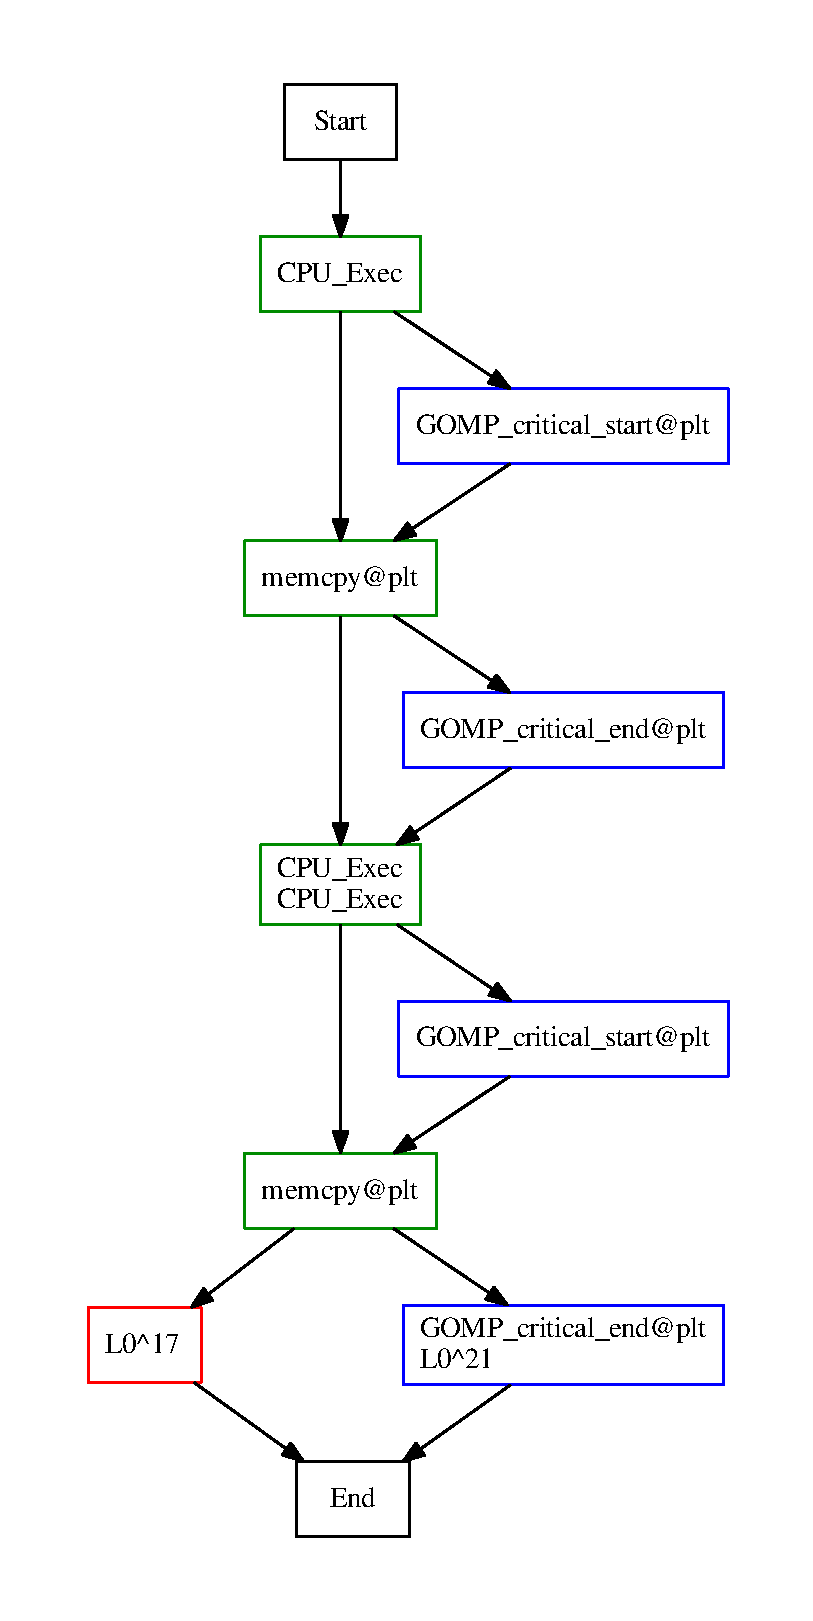
\includegraphics[width=0.3\textwidth]{figs/diffNLR/ompBug-6-4.pdf}
%\caption{OpenMP Bug: diffNLR(6.4)}
%\label{diffNLR-6-4}
%\end{figure}


\subsection{MPI Bug: Deadlock Caused by Fault in Collective}

By forcing process 2 to invoke MPI\_Allreduce (line 24) with a wrong size, we can inject a \textit{real deadlock}.
%
Because the deadlock happens early in the execution, the resulting traces are very different from their fault-free counterparts.
%
Consequently, DiffTrace marks almost all processes as suspicious (cf.~Table~\ref{tab:ar1-ws-all-nn}).
%
Clearly, this is not helpful for debugging.
%
Nevertheless, diffNLR still yields useful information.
%
Since most of the traces are suspicious, we do not know which one the real culprit is and randomly selected trace~4.
%
%It turned out that ParLoT did not happen to capture function calls from all processes since the bug happens too early in the code. Thus except for process 1 and 4, all other traces are empty.
%
By looking at the diffNLR(4) output shown in Figure~\ref{diffNLR-0}, we immediately see that both the normal and the buggy trace are identical up to the invocation of MPI\_Allreduce. This gives the user the first (correct) hint as to where the problem lies.
%
Beyond this point, the bug-free process continues to the end of the program
(it reaches the MPI\_Finalize call) whereas the buggy process does not. The last entry in the buggy trace is a call to MPI\_Allreduce (the last green box), indicating that this call never returned, that is, it deadlocked. This provides the user with the second (correct) hint as to the type of the underlying bug.
%

%
\begin{table}[b]
\centering
\caption{Ranking table - MPI bug: wrong collective size in process 2}
\label{tab:ar1-ws-all-nn}
\scalebox{0.81}{
\begin{tabular}{|c|c|c|c|c|}
\hline
 Filter              & Attributes   &    B-score & \begin{tabular}[c]{@{}c@{}}Top\\Processes\end{tabular}          & \begin{tabular}[c]{@{}c@{}}Top\\Threads\end{tabular}         \\
\hline
% 11.mem.mpicol.ompcrit.cust.0K10 & sing.log10   &      0.383 & 0 , 7 , 2 , 4 , 5 , 6 , & 1.1 , 1.3 , 1.4 , 3.1 , 3.2 , 3.4 , \\
% 11.mem.mpicol.ompcrit.cust.0K10 & sing.noFreq  &      0.383 & 0 , 7 , 2 , 4 , 5 , 6 , & 1.1 , 1.3 , 1.4 , 3.1 , 3.2 , 3.4 , \\
 11.mpicol.cust.0K10             & sing.log10   &      0.439 & 0, 7, 2, 4, 5, 6  & 1.1, 1.3, 3.1, 3.2, 3.4        \\
 11.mpicol.cust.0K10             & sing.noFreq  &      0.439 & 0, 7, 2, 4, 5, 6  & 1.1, 1.3, 3.1, 3.2, 3.4        \\
 11.mpi.cust.0K10                & doub.noFreq  &      0.457 & 0, 7, 2, 4, 5, 6  & 1.4, 3.3, 3.4                    \\
 11.mpi.cust.0K10                & doub.actual  &      0.457 & 0, 7, 2, 4, 5, 6  & 1.4, 3.3, 3.4                    \\
 11.mpiall.cust.0K10             & doub.noFreq  &      0.457 & 0, 7, 2, 4, 5, 6  & 1.4, 3.3, 3.4                    \\
 11.mpiall.cust.0K10             & doub.actual  &      0.457 & 0, 7, 2, 4, 5, 6  & 1.4, 3.3, 3.4                    \\
 11.mpicol.cust.0K10             & doub.noFreq  &      0.457 & 0, 7, 2, 4, 5, 6  & 1.4, 3.3, 3.4                    \\
 11.mpicol.cust.0K10             & doub.actual  &      0.457 & 0, 7, 2, 4, 5, 6  & 1.4, 3.3, 3.4                    \\
 11.mpi.cust.0K10                & sing.log10   &      0.465 & 0, 7, 2, 4, 5, 6  & 1.1, 1.3, 3.1, 3.2, 3.4        \\
 11.mpi.cust.0K10                & sing.noFreq  &      0.465 & 0, 7, 2, 4, 5, 6  & 1.1, 1.3, 3.1, 3.2, 3.4        \\
 11.mpiall.cust.0K10             & sing.log10   &      0.465 & 0, 7, 2, 4, 5, 6  & 1.1, 1.3, 3.1, 3.2, 3.4        \\
 11.mpiall.cust.0K10             & sing.noFreq  &      0.465 & 0, 7, 2, 4, 5, 6  & 1.1, 1.3, 3.1, 3.2, 3.4        \\
 11.mpi.cust.0K10                & doub.noFreq  &      0.543 & 0, 7, 2, 4, 5, 6  & 1.4, 3.3, 3.4                    \\
 11.mpi.cust.0K10                & doub.actual  &      0.543 & 0, 7, 2, 4, 5, 6  & 1.4, 3.3, 3.4                    \\
\hline
\end{tabular}}
\end{table}


%\begin{figure}[]
%\centering
%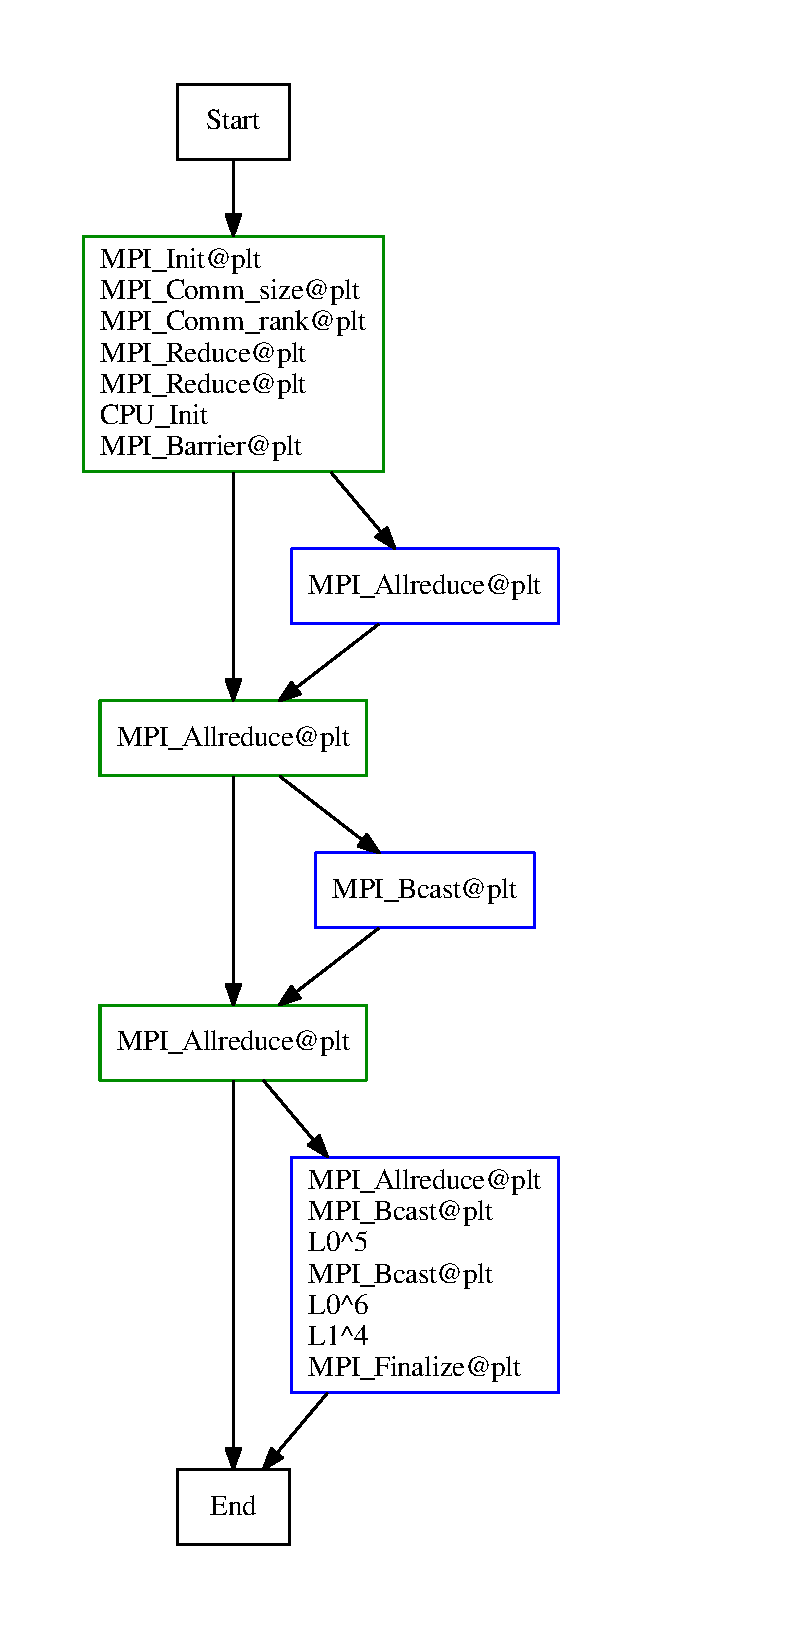
\includegraphics[width=0.3\textwidth]{figs/diffNLR/mpiBug-all-nn.pdf}
%\caption{diffNLR(0)}
%\label{diffNLR-0}
%\end{figure}
%





\subsection{MPI Bug: Wrong Collective Operation}

By changing the MPI\_MIN argument to MPI\_MAX in the MPI\_Allreduce call on line 24 of Listing~\ref{lst:ilcs}, the semantics of ILCS change.
%
Instead of computing the best answer, the modified code computes the worst answer.
%
Hence, this code variation terminates but is likely to yield the wrong result.
%
We injected this bug into process 0.

The first few suspicious processes listed in Table~\ref{tab:ar1-wo-0-nn} are inconclusive. However, the filters that include MPI all agree that process 5 changed the most.
%
Looking at the corresponding diffNLR(5) output in Figure~\ref{diffNLR-5} makes it clear why process 5 was singled out. In the buggy run, it executes many more MPI\_Bcast calls than in the bug-free run because the frequency in which local ``optimums'' are produced has changed. Though this should affect all traces equally, which has reflected in the diffNLR of other traces. We are presenting these tables and figures to show that DiffTrace can reveal the impact of silent bugs like the wrong operation. Such data representation via suggested tables and diffNLRs helps developers to gain insight into the general behavior of the execution. More accurate results can be obtained by refining the parameters and collecting more profound traces (e.g., ParLOT(all images)). This would be part of our future work to find the set of parameters for different classes of bugs to maximize accuracy.



%\begin{figure}[]
%\centering
%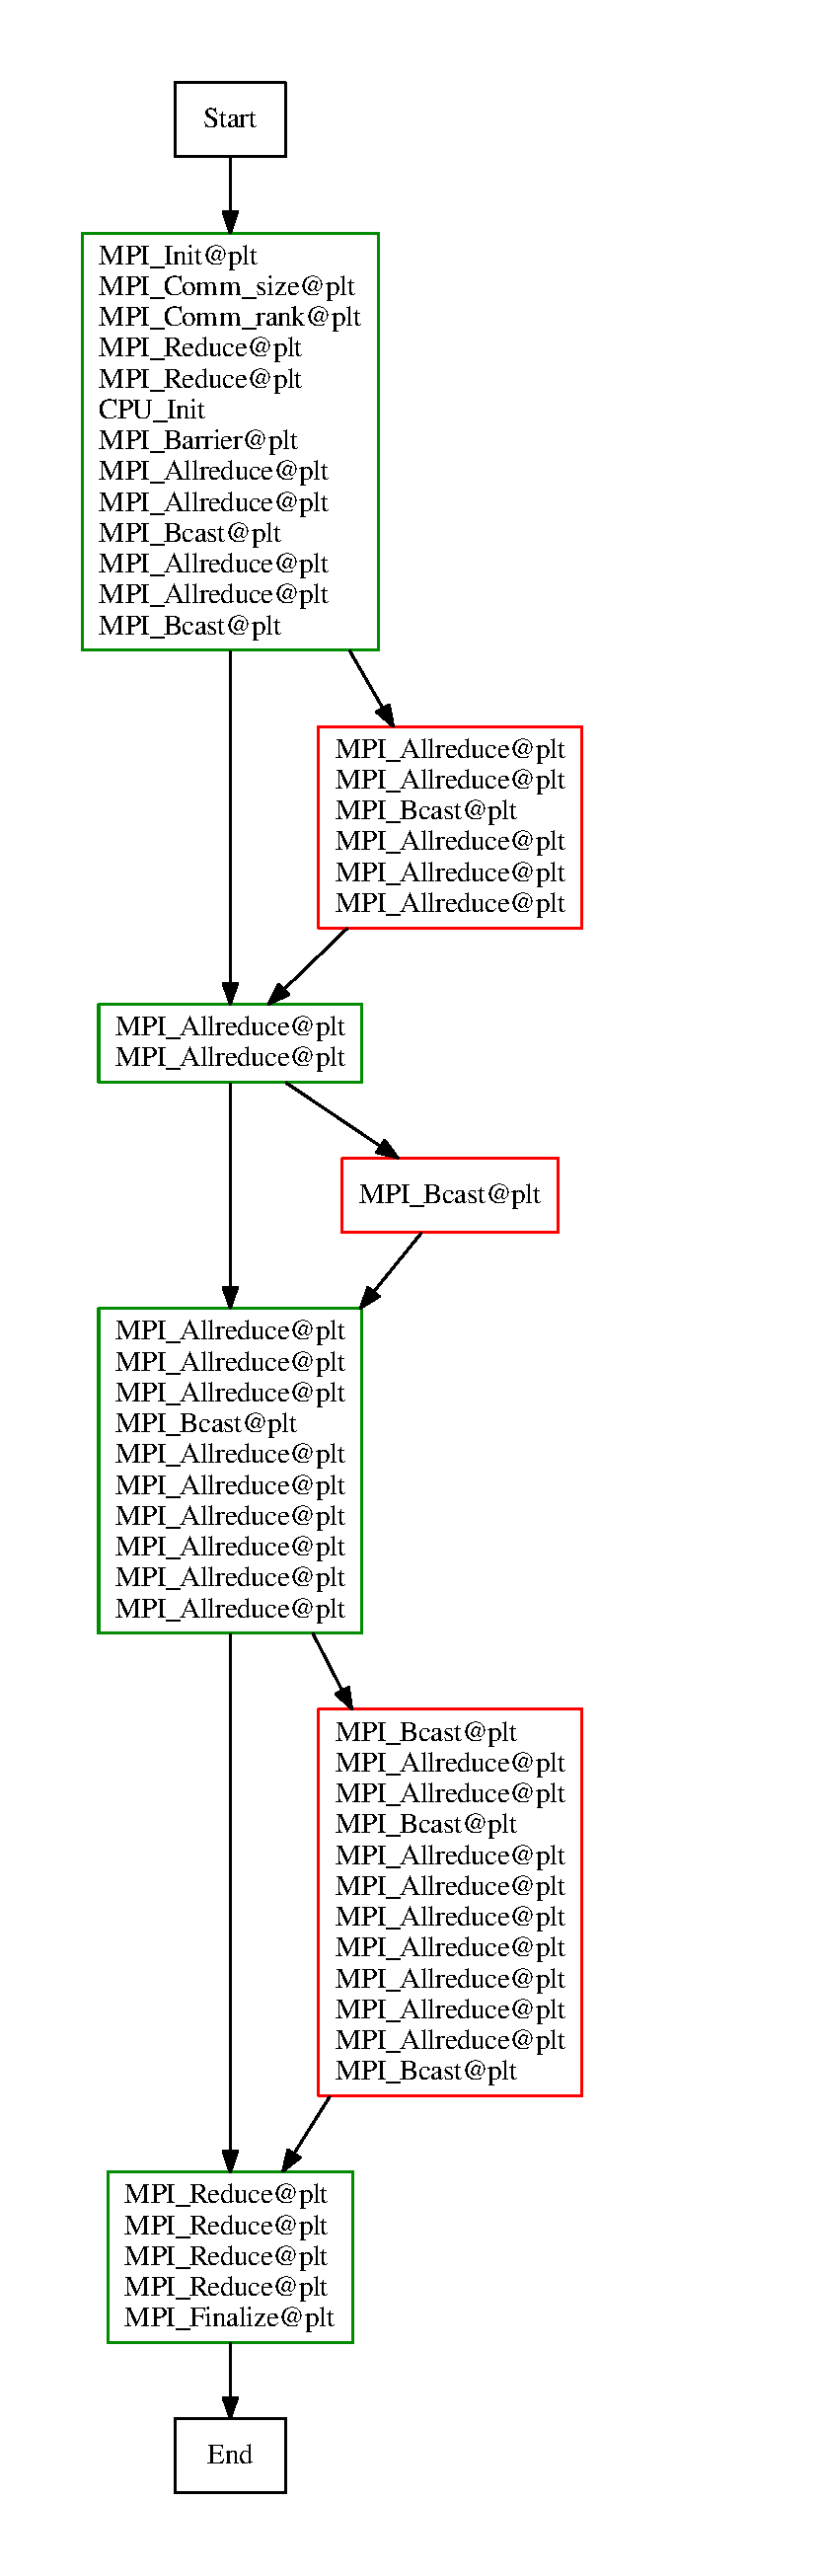
\includegraphics[width=0.3\textwidth]{figs/diffNLR/mpiBug2-0-nn.pdf}
%\caption{diffNLR(5)}
%\label{diffNLR-5}
%\end{figure}

%\begin{table}[]
\centering
\caption{ilcsTSP.mc1-mc-6-n1.m.8.auto}
\label{s1}
\scalebox{0.5}{
\begin{tabular}{lllrrll}
\hline
 Filter                           & Attributes   & Link Method   &   Thresh &   B-score & Top Procs (JSMD)   & TOP Threads(JSMD)                   \\
\hline
 01.mem.ompall.cust.0K10          & sing.actual  & average       &        4 &  0.308594 &                    & 6.2 , 6.4 , 5.2 , 5.4 , 7.3 ,       \\
 11.mem.ompall.cust.0K10          & sing.actual  & average       &        4 &  0.308594 &                    & 6.2 , 6.4 , 5.2 , 5.4 , 7.3 ,       \\
 01.mem.ompmutex.cust.0K10        & sing.actual  & weighted      &        4 &  0.321883 &                    & 6.2 , 3.4 , 5.3 , 4.2 , 7.4 ,       \\
 11.mem.ompmutex.cust.0K10        & sing.actual  & weighted      &        4 &  0.321883 &                    & 6.2 , 3.4 , 5.3 , 4.2 , 7.4 ,       \\
 11.plt.mem.mpi.ompcrit.cust.0K10 & doub.actual  & weighted      &        4 &  0.324427 & 3 ,                & 0.2 , 1.1 , 3.1 , 4.3 , 4.4 , 5.2 , \\
 01.plt.mem.mpi.ompcrit.cust.0K10 & doub.actual  & weighted      &        4 &  0.324427 & 3 ,                & 0.2 , 1.1 , 3.1 , 4.3 , 4.4 , 5.2 , \\
 01.mem.ompall.cust.0K10          & doub.actual  & weighted      &        4 &  0.33266  & 3 ,                & 6.4 , 7.1 , 3.4 , 4.3 , 4.4 , 5.2 , \\
 11.mem.ompall.cust.0K10          & doub.actual  & weighted      &        4 &  0.33266  & 3 ,                & 6.4 , 7.1 , 3.4 , 4.3 , 4.4 , 5.2 , \\
 01.mem.ompcrit.cust.0K10         & sing.actual  & weighted      &        4 &  0.354396 & 6 ,                & 7.2 , 7.4 , 3.4 , 4.2 , 4.3 , 4.4 , \\
 11.mem.ompcrit.cust.0K10         & sing.actual  & weighted      &        4 &  0.354396 & 6 ,                & 7.2 , 7.4 , 3.4 , 4.2 , 4.3 , 4.4 , \\
 11.plt.mem.mpi.ompcrit.cust.0K10 & doub.actual  & average       &        4 &  0.381646 &                    & 3.3 , 2.4 ,                         \\
\hline
\end{tabular}}
\end{table}


\begin{table}[]
\centering
\caption{ilcsTSP.mc1-mc-2-2.m.8.auto}
\label{s2}
\scalebox{0.5}{
\begin{tabular}{lllrrll}
\hline
 Filter                           & Attributes   & Link Method   &   Thresh &   B-score & Top Procs (JSMD)   & TOP Threads(JSMD)                   \\
\hline
 01.mem.ompall.cust.0K10          & doub.actual  & weighted      &        4 &  0.309391 & 3 ,                & 6.2 , 6.4 , 7.1 , 7.4 , 1.3 , 3.1 , \\
 11.mem.ompall.cust.0K10          & doub.actual  & weighted      &        4 &  0.309391 & 3 ,                & 6.2 , 6.4 , 7.1 , 7.4 , 1.3 , 3.1 , \\
 11.plt.mem.cust.0K10             & doub.actual  & weighted      &        4 &  0.318003 & 7 , 4 ,            & 1.3 , 2.2 , 3.3 , 3.4 , 4.2 , 4.3 , \\
 01.plt.mem.cust.0K10             & doub.actual  & weighted      &        4 &  0.318003 & 7 , 4 ,            & 1.3 , 2.2 , 3.3 , 3.4 , 4.2 , 4.3 , \\
 01.mem.ompall.cust.0K10          & doub.actual  & average       &        4 &  0.34462  & 7 , 3 ,            & 7.1 , 1.3 , 1.4 , 2.2 , 2.3 , 3.1 , \\
 11.mem.ompall.cust.0K10          & doub.actual  & average       &        4 &  0.34462  & 7 , 3 ,            & 7.1 , 1.3 , 1.4 , 2.2 , 2.3 , 3.1 , \\
 11.plt.mem.mpi.ompcrit.cust.0K10 & doub.actual  & average       &        4 &  0.350702 & 7 , 3 ,            & 6.2 , 6.3 , 7.2 , 2.4 , 3.3 , 4.2 , \\
 01.plt.mem.mpi.ompcrit.cust.0K10 & doub.actual  & average       &        4 &  0.350702 & 7 , 3 ,            & 6.2 , 6.3 , 7.2 , 2.4 , 3.3 , 4.2 , \\
 11.plt.mem.cust.0K10             & doub.actual  & weighted      &        3 &  0.357334 & 7 ,                & 2.2 , 3.3 , 3.4 , 4.3 , 4.4 ,       \\
 01.plt.mem.cust.0K10             & doub.actual  & weighted      &        3 &  0.357334 & 7 ,                & 2.2 , 3.3 , 3.4 , 4.3 , 4.4 ,       \\
 01.mem.ompall.cust.0K10          & doub.actual  & weighted      &        3 &  0.380481 & 3 ,                & 7.1 , 1.3 , 3.1 , 4.3 , 4.4 ,       \\
\hline
\end{tabular}}
\end{table}


\begin{table}[]
\centering
\caption{ilcsTSP.ar2-wo-2-nn.m.8.auto}
\label{s3}
\scalebox{0.5}{
\begin{tabular}{lllrrll}
\hline
 Filter           & Attributes   & Link Method   &   Thresh &   B-score & Top Procs (JSMD)   & TOP Threads(JSMD)                   \\
\hline
 01.plt.cust.0K10 & doub.actual  & average       &        4 &  0.392446 & 6 ,                & 2.3 , 2.4 , 4.2 , 4.3 , 4.4 ,       \\
 11.plt.cust.0K10 & doub.actual  & average       &        4 &  0.392446 & 6 ,                & 2.3 , 2.4 , 4.2 , 4.3 , 4.4 ,       \\
 01.plt.cust.0K10 & sing.log10   & centroid      &        4 &  0.945946 & 0 ,                & 6.2 , 0.4 , 1.1 , 0.1 , 2.3 , 2.4 , \\
 01.plt.cust.0K10 & sing.log10   & median        &        4 &  0.945946 & 0 ,                & 6.2 , 0.4 , 1.1 , 0.1 , 2.3 , 2.4 , \\
 11.plt.cust.0K10 & sing.log10   & centroid      &        4 &  0.945946 & 0 ,                & 6.2 , 0.4 , 1.1 , 0.1 , 2.3 , 2.4 , \\
 11.plt.cust.0K10 & sing.log10   & median        &        4 &  0.945946 & 0 ,                & 6.2 , 0.4 , 1.1 , 0.1 , 2.3 , 2.4 , \\
 01.plt.cust.0K10 & sing.log10   & median        &        3 &  0.947368 & 0 ,                & 6.2 , 0.4 , 1.1 , 0.1 , 2.3 , 2.4 , \\
 11.plt.cust.0K10 & sing.log10   & median        &        3 &  0.947368 & 0 ,                & 6.2 , 0.4 , 1.1 , 0.1 , 2.3 , 2.4 , \\
 01.plt.cust.0K10 & sing.log10   & complete      &        3 &  1        & 0 ,                & 0.1 , 7.1 , 1.1 , 3.1 , 3.3 ,       \\
 01.plt.cust.0K10 & sing.log10   & complete      &        4 &  1        & 0 ,                & 0.1 , 7.1 , 1.1 , 3.1 , 3.3 ,       \\
 01.plt.cust.0K10 & sing.log10   & average       &        4 &  1        & 0 ,                & 0.1 , 7.1 , 1.1 , 3.1 , 3.3 ,       \\
\hline
\end{tabular}}
\end{table}


\begin{table}[]
\centering
\caption{ilcsTSP.bc2-wr-3-nn.m.8.auto}
\label{s4}
\scalebox{0.5}{
\begin{tabular}{lllrrll}
\hline
 Filter              & Attributes   & Link Method   &   Thresh &   B-score & Top Procs (JSMD)   & TOP Threads(JSMD)                   \\
\hline
 01.plt.cust.0K10    & doub.actual  & centroid      &        4 &  0.512309 & 2 ,                & 6.4 , 7.3 , 1.2 , 1.3 , 2.1 , 2.2 , \\
 11.plt.cust.0K10    & doub.actual  & centroid      &        4 &  0.512309 & 2 ,                & 6.4 , 7.3 , 1.2 , 1.3 , 2.1 , 2.2 , \\
 01.plt.cust.0K10    & sing.actual  & average       &        4 &  0.513221 & 7 ,                & 3.4 , 5.2 , 4.2 , 4.3 ,             \\
 11.plt.cust.0K10    & sing.actual  & average       &        4 &  0.513221 & 7 ,                & 3.4 , 5.2 , 4.2 , 4.3 ,             \\
 11.mpi.cust.0K10    & sing.actual  & median        &        4 &  0.544807 & 0 ,                & 0.1 , 6.4 , 7.3 , 7.4 , 1.3 , 0.2 , \\
 11.mpiall.cust.0K10 & sing.actual  & median        &        4 &  0.544807 & 0 ,                & 0.1 , 6.4 , 7.3 , 7.4 , 1.3 , 0.2 , \\
 01.mpiall.cust.0K10 & sing.actual  & median        &        4 &  0.544807 & 0 ,                & 0.1 , 6.4 , 7.3 , 7.4 , 1.3 , 0.2 , \\
 01.mpicol.cust.0K10 & sing.actual  & median        &        4 &  0.544807 & 0 ,                & 0.1 , 6.4 , 7.3 , 7.4 , 1.3 , 0.2 , \\
 11.mpicol.cust.0K10 & sing.actual  & median        &        4 &  0.544807 & 0 ,                & 0.1 , 6.4 , 7.3 , 7.4 , 1.3 , 0.2 , \\
 01.mpi.cust.0K10    & sing.actual  & median        &        4 &  0.544807 & 0 ,                & 0.1 , 6.4 , 7.3 , 7.4 , 1.3 , 0.2 , \\
 01.plt.cust.0K10    & doub.actual  & centroid      &        3 &  0.639268 & 2 ,                & 6.4 , 7.3 , 1.2 , 1.3 , 2.1 , 2.2 , \\
\hline
\end{tabular}}
\end{table}

\begin{table}[]
\centering
\caption{ilcsTSP.bc1-ws-3-nn.m.8.auto}
\label{s5}
\scalebox{0.5}{
\begin{tabular}{lllrrll}
\hline
 Filter              & Attributes   & Link Method   &   Thresh &   B-score & Top Procs (JSMD)   & TOP Threads(JSMD)                   \\
\hline
 11.mpi.cust.0K10    & sing.actual  & weighted      &        4 &  0.385229 & 6 ,                & 6.2 , 6.3 , 6.4 , 7.2 , 7.3 , 7.4 , \\
 11.mpiall.cust.0K10 & sing.actual  & weighted      &        4 &  0.385229 & 6 ,                & 6.2 , 6.3 , 6.4 , 7.2 , 7.3 , 7.4 , \\
 01.mpiall.cust.0K10 & sing.actual  & weighted      &        4 &  0.385229 & 6 ,                & 6.2 , 6.3 , 6.4 , 7.2 , 7.3 , 7.4 , \\
 01.mpicol.cust.0K10 & sing.actual  & weighted      &        4 &  0.385229 & 6 ,                & 6.2 , 6.3 , 6.4 , 7.2 , 7.3 , 7.4 , \\
 11.mpicol.cust.0K10 & sing.actual  & weighted      &        4 &  0.385229 & 6 ,                & 6.2 , 6.3 , 6.4 , 7.2 , 7.3 , 7.4 , \\
 01.mpi.cust.0K10    & sing.actual  & weighted      &        4 &  0.385229 & 6 ,                & 6.2 , 6.3 , 6.4 , 7.2 , 7.3 , 7.4 , \\
 01.plt.cust.0K10    & sing.actual  & weighted      &        4 &  0.448188 & 7 , 3 ,            & 6.2 , 6.4 , 7.1 , 7.4 , 3.3 , 3.4 , \\
 11.plt.cust.0K10    & sing.actual  & weighted      &        4 &  0.448188 & 7 , 3 ,            & 6.2 , 6.4 , 7.1 , 7.4 , 3.3 , 3.4 , \\
 11.mpi.cust.0K10    & sing.actual  & weighted      &        3 &  0.465043 & 6 ,                & 6.2 , 6.3 , 6.4 , 7.2 , 7.3 , 7.4 , \\
 11.mpiall.cust.0K10 & sing.actual  & weighted      &        3 &  0.465043 & 6 ,                & 6.2 , 6.3 , 6.4 , 7.2 , 7.3 , 7.4 , \\
 01.mpiall.cust.0K10 & sing.actual  & weighted      &        3 &  0.465043 & 6 ,                & 6.2 , 6.3 , 6.4 , 7.2 , 7.3 , 7.4 , \\
\hline
\end{tabular}}
\end{table}


\section{LULESH2 Examples}
\label{sec:ch3_lulesh}

% study of LULESH (prelim)

Our ultimate goal is to apply DiffTrace to complex HPC codes.
%
As a more complex example, we have executed the single-cycle LULESH2\cite{LULESH2:changes} with 8 MPI processes
and 4 OMP threads (system configuration described in \S\ref{sec:ilcs-case-study})
and collected ParLOT (main image) function calls.


Before bug injection, we analyzed LULESH2 traces and computed some statistics to gain insight into the
general control flow of LULESH2 and also to evaluate DiffTrace's
performance and effectiveness.
%
Our primary results show that ParLOT instruments and captures \textbf{410 distinct function} calls on
average per process, and stores them in compressed trace files of size less than \textbf{2.8 KB}
on average per thread.
%
Upon decompression, each per process trace file
turns into a sequence of \textbf{421503} function calls on average. The equivalent NLR of each trace file reduces the sequence size by a factor of \textbf{1.92} and \textbf{16.74}, for constant $K$ set to 10 and 50, respectively.
%
%We let DiffTrace preprocess traces without ignoring or filtering any of the functions, convert them into their equivalent NLRs, and generate concept lattices and JSMs.
%
%With NLR constant $K$ set to 10, the average NLR compression ratio is \textbf{1.92}, while the process of loop detection took about 260 seconds to complete per trace.
%
%By increasing $K$ to 50, the NLR compression ratio drastically shifted up to \textbf{16.74} on average.
%
%However, it took more than an hour for DiffTrace to convert each trace to its equivalent NLR.
%
%The decompression and concept lattice generation times were not significant (e.g., a few milliseconds).


For further evaluation of DiffTrace, we injected a fault into the LULESH source code so that the process with rank 2
would not invoke the function \texttt{LagrangeLeapFrog} that is in charge of updating ``domain'' distances and send/receive
MPI messages from other processes.
%

%
Table \ref{tab:lulesh} reflects the ID of processes (rightmost column)
that DiffTrace's ranking system suggests as the most affected traces by the bug.
%
Since the fault in process 2 prevents other processes from making progress and successfully terminate,
all of the process IDs appeared in the table.
The generated diffNLRs clearly showed the point at which each process stopped making progress.
%
Due to lack of space, we did not include the relatively large diffNLRs of LULESH in this paper.
However, all diffNLRs and related observations are available online via~\cite{diffTraceMaterials}.
\begin{table}[t]
\centering
\caption{Ranking Table for LULESH}
\label{tab:lulesh}
\scalebox{1.01}{
\begin{tabular}{|l|l|r|l|}
\hline
 Filter   & Attributes   &  B-score & Top Processes        \\
\hline
 11.1K10  & sing.noFreq  &    0.295 & \textbf{2} , 3 , 4 , 5 , 6 , 7   \\
 01.1K10  & sing.noFreq  &    0.354 & 0 , 1 , \textbf{2} , 3 , 4 , 5   \\
 01.1K10  & sing.actual  &    0.383 & \textbf{2} , 3 , 4 , 5 , 6 , 7   \\
 11.1K10  & sing.noFreq  &    0.408 & \textbf{2} , 3 , 4 , 5 , 6 , 7   \\
 11.1K10  & sing.noFreq  &    0.408 & \textbf{2} , 3 , 4 , 5 , 6 , 7   \\
 01.1K10  & doub.noFreq  &    0.433 & 4 , 5 , 6               \\
 01.1K10  & doub.noFreq  &    0.433 & 4 , 5 , 6               \\
 11.1K10  & doub.noFreq  &    0.433 & 5 , 1 , 6               \\
 01.1K10  & doub.noFreq  &    0.455 & 1 , \textbf{2} , 3 , 4 , 7       \\
 11.1K10  & doub.noFreq  &    0.458 & 5 , 1 , 6               \\
 11.1K10  & doub.noFreq  &    0.458 & 4 , 5 , 6 , 7           \\
 01.1K10  & sing.log10   &    0.459 & 1 , \textbf{2} , 3 , 4 , 5 , 6   \\
 01.1K10  & doub.noFreq  &    0.472 & 0 , 1 , \textbf{2} , 3 , 4 , 5   \\
 01.1K10  & sing.log10   &    0.475 & 1 , 3 , 4 , 5 , 6 , 7   \\
 01.1K10  & sing.log10   &    0.478 & 1 , \textbf{2} , 3 , 4 , 5 , 6   \\
 01.1K10  & sing.log10   &    0.478 & 1 , \textbf{2} , 3 , 4 , 5 , 6   \\
\hline
\end{tabular}}
\end{table}



\section{Related Work}
\label{sec:ch3_related}
Three major recent studies
have emphasized the need for better debugging tools
{\em and} the need to build a community that can share debugging
methods and infrastructure: the DOE report mentioned
earlier \cite{hpcdoe},
an NSF workshop~\cite{Cohen:2018:IRC:3297279}, and an ASCR report on
extreme heterogeneity~\cite{ascr-report-extreme-heterogeneity}.
%
Our key contribution in this paper is a fresh approach to debugging
that (1)~incorporates methods to debug across the API-stack
by resorting to binary tracing and thereby being able to ``dial into''
MPI bugs and/or OpenMP bugs (as shown in the ILCS case study), (2)~makes
initial triage of debugging methods possible via function-call traces,
and (3)~enables the verification community to cohere around DiffTrace
by allowing other tools to extend our toolchain (they can tap into it at various places).


Many HPC debugging efforts have emphasized
the need to highlight dissimilarities and
incorporate progress measures on loops. We now
summarize a few of them.
%
AutomaDeD~\cite{automaded-GBron}\cite{automaded-laguna}
captures the application's control flow
via Semi Markov Models and detects outlier executions.
%
PRODOMETER~\cite{prodometer} detects loops in
AutomaDeD models and introduces the
notion of {\em least progressed tasks} by analyzing {\em progress dependency graphs}.
%
DiffTrace's DiffNLR method does not (yet) incorporate progress measures; it only
computes changes in loop {\em structure}.
%
Prodometer's methods are ripe for symbiotic incorporation into DiffTrace.
%
We also plan to incorporate {\em happens-before} computation as a progress measure using FCA-based algorithms by Garg et al.~\cite{latticeForDistConst,garg_2015}.
%
FCA-based approaches have been widely used in data mining~\cite{cldm},
machine learning~\cite{clml}, and information retrieval \cite{ignatov17}.


In terms of computing differences with previous executions,
we draw inspirations from
Zeller's delta-debugging~\cite{DBLP:conf/esec/Zeller99}
and De Rose et al.'s relative debugging~\cite{relative-debugging}.
%
The power of equivalence classes for outlier detection is
researched in STAT~\cite{stat}, which
merges stack traces from processes into a prefix tree,
looking for equivalence-class outliers.
%
STAT uses the StackWalker API from Dyninst~\cite{dyninst} to gather stack traces
and efficiently handles scaling issues
through tree-based overlay networks such as MRnet~\cite{mrnet}.
%
D4~\cite{liu-18} detects concurrency bugs by statically analyzing source-code
changes, and DMTracker~\cite{dmtracker} detects anomalies in data movement.
%
The communication patterns of HPC applications can be automatically characterized by
diffing the communication matrix with common patterns~\cite{roth-15} or by
detecting repetitive patterns~\cite{preissl-08}.
%
ScalaTrace~\cite{scalatrace} captures and compresses communication traces for later replay. 
%
Synoptic~\cite{beschastnikh-synoptic} is applied to distributed
system logs to find bugs.
%
%Ravel~\cite{ravel} systematically visualizes large-scale application communications~\cite{charmVis}. 

%
%
%\subsection{OTHERS}
%\hl{in case of lack of material}
%\begin{itemize}
%\item Trace File Comparison with a hierarchical Sequence Alignment algorithm \cite{weber-seqAlign}
%\item structural clustering : matthias weber \cite{weberStructural}
%\item building a better backtrace: techniques for postmortem program analysis - ben liblit \cite{liblit02}
%\item automatically charecterizing large scale program behavior - timothy sherwood \cite{sherwood02}
%\item Score-P \cite{scorep}
%\item TAU \cite{tau}
%\item ScalaTrace: Scalable compression and replay of communication traces for HPC  \cite{scalatrace}
%\end{itemize}






%
%\subsection{STAT}
%
%Parallel debugger STAT\cite{stat}
%\begin{itemize}
%\item STAT gathers stack traces from all processes
%\item Merge them into prefix tree
%\item Groups processes that exhibit similar behavior into equivalent classes
%\item A single representative of each equivalence can then be examined with a full-featured debugger like TotalView or DDT
%\end{itemize}
%
%What STAT does not have?
%
%\begin{itemize}
%\item FP debugging
%\item Portability (too many dependencies)
%\item Domain-specific
%\item Loop structures and detection
%\end{itemize}




\section{Discussions \& Future Work}
\label{sec:ch3_discussion}
DiffTrace is the first tool we know of that situates debugging around {\em whole program}
diffing, and~(1)~provides user-selectable front-end filters of function calls to keep;
~(2)~summarizes loops based on state-of-the-art algorithms to detect loop-level
behavioral differences;
~(3)~condenses the loop-summarized
traces into concept lattices that are built using incremental
algorithms;~(4)~and clusters behaviors using hierarchical clustering and ranks them by similarity to detect and highlight the most salient differences.
%a
We deliberately chose the path of a clean start that addresses missing features
in existing tools and missing collectivism in the debugging community.
%
Our initial assessment of this design is encouraging.
%

In our future work we will improve DiffTrace components as follows:
%
%
(1)~Optimizing them to exploit multi-core CPUs, thus reducing the overall analysis time;
%
(2)~Converting ParLOT traces into Open Trace Format (OTF2) by logically timestamping trace entries to mine temporal properties of functions such as \textit{happened-before}~\cite{lamport};
%
(3)~Conducting systematic bug-injection to see whether concept lattices and loop structures can be used as elevated features for precise bug classifications via machine learning and neural network techniques; and
%
(4)~Taking up more challenging and real-world examples to evaluate DiffTrace against similar tools, and release it to the community.
%--end
% leave a blank line

\noindent{\bf Acknowledgements:\/} Supported in part by
NSF awards CCF 1817073 and 1704715.


%%% -*-LaTeX-*-

\chapter{Automated Concurrency Testing Framework for Go}

%%% -*-LaTeX-*-

\chapter{Conclusion and Future Work}
\label{sec:ch5}
This dissertation presented a series of tools that combine concurrent debugging approaches to aid debugging using efficient data collection and automated analysis frameworks.
%
We presented \parlot, a portable low overhead dynamic binary instrumentation-based whole-program tracing approach that can support various dynamic program analyses, including debugging.
%
Key properties of \parlot include its on-the-fly trace collection and compression that reduces timing jitter, I/O bandwidth, and storage requirements to such a degree that whole-program call/return traces can be collected efficiently even at scale.
%
We evaluated various versions of \parlot created by disabling/enabling compression.
%
Our metrics include the tracing overhead, required bandwidth, achieved compression ratio, initialization overhead, and the overall impact of compression.
%
Detailed evaluations on the NAS parallel benchmarks running on up to 1024 cores establish the merit of our tool and our design decisions. \parlot can collect more than 36 MB worth of data per core per second while only needing 56 kB/s of bandwidth and slowing down the application by 2.7x on average.
%
These results are auspicious in supporting whole program tracing and debugging, particularly considering that most of the overhead is due to the DBI tool and not \parlot.
%


We described the design of DiffTrace, the first tool we know of that situates debugging around {\em whole program} diffing, and~(1)~provides user-selectable front-end filters of function calls to keep;
~(2)~summarizes loops based on state-of-the-art algorithms to detect loop-level behavioral differences;
~(3)~condenses the loop-summarized traces into concept lattices that are built using incremental algorithms;~(4)~and clusters behaviors using hierarchical clustering and ranks them by similarity to detect and highlight the most salient differences.
%a

Lastly, we presented \goat, an end-to-end analysis and debugging framework for concurrent Go applications.
%
\goat combines static and dynamic methods to gather evidence about the dynamic behavior of concurrency primitives, model the program's concurrency behavior, and explore the interleaving space to reveal the flaws.
%
\goat detects all 68 blocking bugs of GoKer benchmark, which are the bug kernels adopted from the top nine open-source projects written in Go.
%
Moreover, by defining a set of coverage requirements and dynamic measurement, we quantify the quality of the schedule-space exploration of \goat.
%
Proposed coverage requirements accurately reflect the dynamic behavior of program executions and testing iterations.
%

\section{Future Work}
The following is the list of improvements to be made for each tool and potential future work in dynamic analysis tools.

\subsection{\parlot}
\begin{itemize}
  \item Allowing users to selectively trace at specific interfaces: doing so can further increase compression efficiency
  by reducing the variety of function calls to be handled by
  the compressor.
  \item The need to bring down initialization overheads: experiments show the majority of overhead belongs to the initialization of Pin. Switching to a less general-purpose DBI tool improves the efficiency of \parlot.
\end{itemize}
\subsection{DiffTrace}
In our future work, we will improve DiffTrace components as follows:
%
\begin{itemize}
  \item Optimizing them to exploit multi-core CPUs, thus reducing the overall analysis time.
  \item Converting ParLOT traces into Open Trace Format (OTF2) by logically timestamping trace entries to mine temporal properties of functions such as \textit{happened-before}~\cite{lamport}.
  \item Conducting systematic bug-injection to see whether concept lattices and loop structures can be used as elevated features for precise bug classifications via machine learning and neural network techniques.
  \item Taking up more challenging and real-world examples to evaluate DiffTrace against similar tools and release it to the community.
\end{itemize}
\subsection{\goat}
The engineering of \goat is flexible and extensible to more advanced components. The following is the list of potential improvements to the framework:
\begin{itemize}
  \item The concurrency dynamic tracing of Go applications enables extensive investigation of NLP/ML for concurrent debugging by training models (\eg, word2vec) based on collected traces for automatic anomaly detection.
  \item The \goat API can ``control'' which goroutine to execute next by maintaining the history of executed interleavings and goroutine ids. This way, we can systematically explore all possible interleavings efficiently to achieve a higher coverage percentage.
  \item We are actively developing \goat as an open-source, easy-to-use (within an independent container) testing tool. With the release of \goat, we enable developers to explore the schedule space of their concurrent applications to reveal potential flaws.
\end{itemize}
\subsection{Dynamic Analysis Tools}
The following enumerates a few future directions in dynamic analysis tools for HPC/Cloud community.
\begin{itemize}
  \item Finding the sweet spot between \textit{maximal data collection} and \textit{minimal slowdown} is the key for a dynamic analysis tool to gain acceptance and practical use for real-world and large-scale applications. Picking the right data to collect maximizes the trade-off.
  \item Both static and dynamic analysis tools have advantages and limitations. Complementing ideas from both sides help to achieve a high degree of confidence about the program's bug freedom while enabling practical use of the tool in production languages.
  \item It is not feasible to put the developer completely out of the ``debugging'' loop through fully automated mechanisms. Tools may produce false positives and miss bugs that did not occur. It is the developer's task to achieve a high degree of confidence in her software. If a bug is revealed during testing or verification, the developer needs to fix the bug or incorporate the suggested fix. In other words, the developer is the one who closes the debugging circle and delivers the software. Middleware tools like \parlot, DiffTrace, and \goat, which provide a human-readable representation of dynamic behavior of complex programs, can drastically reduce the cost of debugging.
\end{itemize}

%%%% -*-LaTeX-*-

\chapter{The Third}

This is a chapter.

\blah

%%%% -*-LaTeX-*-

\chapter{The Fourth}

This is a chapter.

\blah

\blah

\blah

\section{More on the topic}

\blah

\blah

\section{Even more on the topic}

\blah

\blah

\section{Summary and conclusions}

\blah


% \numberofappendices = 1   % Set 0 for none, else number of appendices.
%\numberofappendices = 3
%\appendix       % Chapters, sections are now appendix style A, A.1, A.2, B, C, D, ...

%%%% -*-LaTeX-*-

\chapter{The First}

This is an appendix.  Notice that the \LaTeX{} markup for an appendix
is, surprisingly, \verb=\chapter=.  The \verb=\appendix= command does
not produce a heading; instead, it just changes the numbering style
from numeric to alphabetic, and it changes the heading prefix from
\textbf{CHAPTER} to \textbf{APPENDIX}.

\blah \blah \blah

%%%% -*-LaTeX-*-

\chapter{The Second}

This is an appendix.

\blah \blah \blah

%%%% -*-LaTeX-*-

\chapter{The Third}

This is an appendix.

There are several books
\cite{%
    Singh:1997:FEE,%
    Salomon:1995:AT,%
    Robbins:2005:CSS,%
    Randell:1982:ODC,%
    Olver:2010:NHM,%
    Mittelbach:2004:LC,%
    Lamport:1985:LDP,%
    Knuth:1999:DT,%
    Knuth:1986:TB,%
    Knuth:1986:MB,%
    Farmelo:2009:SMH%
}
listed in our bibliography.

We also reference several journal articles
\cite{%
    Wiles:1995:MEC,%
    Taylor:1995:RTP,%
    Lahiri:2002:ADA,%
    Kim:1999:AFC,%
    Johnson:1978:LDT,%
    Huskey:1980:LLC,%
    Heilbron:1969:GBA,%
    Hall:1994:PNE,%
    Goldstine:1946:ENI,%
    Einstein:1911:BMAb,%
    Einstein:1911:BMAa,%
    Einstein:1906:NBM,%
    Cody:1981:APF,%
    Beebe:1989:PCP,%
    Babbage:1910:BBA%
}
and three famous doctoral theses of later winners
\cite{%
    Einstein:1905:NBM,%
    Dirac:1926:QM,%
    Bohr:1911:SME%
}
of the Nobel Prize in Physics (1922, 1933, and
1921):

Notice that, even though those citations appeared
in \LaTeX{} \verb=\cite{...}= commands with their
\BibTeX{} citation labels in reverse alphabetical
order, thanks to the \verb=citesort= package,
their reference-list numbers have been sorted in
numerically ascending order, and then
range-reduced.

Mention should also be made of a famous Dutch
computer scientist's first publication
\cite{Dijkstra:1953:FBV}.

Font metrics are an important, albeit low-level,
aspect of typesetting. See the \emph{Adobe
Systems} manual about that company's procedures
\cite{Adobe:1990:AFM}.

The bibliography at the end of this thesis contains several examples
of documents with non-English titles, and their \BibTeX{} entries
provide title translations following the practice recommended by the
American Mathematical Society and SIAM\@.  Here is a sample entry that
shows how to do so:
%
\begin{verbatim}
@PhdThesis{Einstein:1905:NBM,
  author =       "Albert Einstein",
  title =        "{Eine Neue Bestimmung der Molek{\"u}ldimensionen}.
                 ({German}) [{A} new determination of molecular
                 dimensions]",
  type =         "Inaugural dissertation",
  school =       "Bern Wyss.",
  address =      "Bern, Switzerland",
  year =         "1905",
  bibdate =      "Fri Dec 17 10:46:57 2004",
  bibsource =    "http://www.math.utah.edu/pub/tex/bib/einstein.bib",
  note =         "Published in \cite{Einstein:1906:NBM}.",
  acknowledgement = ack-nhfb,
  language =     "German",
  advisor =      "Alfred Kleiner (24 April 1849--3 July 1916)",
  URL =          "http://en.wikipedia.org/wiki/Alfred_Kleiner",
  remark =       "Received August 19, 1905 and published February 8,
                 1906.",
  Schilpp-number = "6",
}
\end{verbatim}

The \texttt{note} field in that entry refers to another bibliography
entry that need not have been directly cited in the document text.
Such cross-references are common in \BibTeX{} files, especially for
journal articles where there may be later comments and corrigenda that
should be mentioned.  Embedded \verb=\cite{}= commands ensure that
those possibly-important other entries are always included in the
reference list when the entry is cited.  The last bibliography entry
\cite{Wiles:1995:MEC} in this thesis has a long \texttt{note} field
that tells more about what some may view as the most important paper
in mathematics in the last century.

When entries cite other entries that cite other entries that cite
other entries that \ldots{}, multiple passes of \LaTeX{} and \BibTeX{}
are needed to ensure consistency.  That is another reason why document
compilation should be guided by a \texttt{Makefile} or a batch script,
rather than expecting the user to remember just how many passes are
needed.

\BibTeX{} entries are \emph{extensible}, in that arbitrary key\slash
value pairs may be present that are not necessarily recognized by any
bibliography style files.  The \texttt{advisor},
\texttt{acknowledgement}, \texttt{bibdate}, \texttt{bibsource},
\texttt{language}, \texttt{remark}, and \texttt{Schilpp-number} fields
are examples, and may be used by other software that processes
\BibTeX{} entries, or by humans who read the entries.  \texttt{DOI}
and \texttt{URL} fields are currently recognized by only a few styles,
but that situation will likely change as publishers demand that such
important information be included in reference lists.

In \BibTeX{} \texttt{title} fields, braces protect words, such as
proper nouns and acronyms, that cannot be downcased if the selected
bibliography style would otherwise do so.  In German, all nouns are
capitalized, and the simple way to ensure their protection is to brace
the entire German text in the title, as we did in the entry above.

The world's first significant computer program may
have been that written in 1842 by Lady Augusta Ada
Lovelace (1815--1852) for the computation of Bernoulli
numbers \cite{Huskey:1980:LLC,Kim:1999:AFC}.  She
was the assistant to Charles Babbage
(1791--1871), and they are the world's first
computer programmers. The programming language
\emph{Ada} is named after her, and is defined in
the ANSI/MIL-STD-1815A Standard; its number
commemorates the year of her birth.

We do not discuss mathematical \emph{transforms}
in this dissertation, but you can find that phrase
in the index (except that this sample thesis doesn't have one!)

\blah

\blah
\blah

\blah


%%% The choice of bibliography style is a major decision, jointly made
%%% by you, your thesis advisor and the thesis editor. Common choices are
%%% one of the four standard BibTeX styles (abbrv, alpha, plain, and unsrt),
%%% or enhanced styles like acm, amsplain, siam, and hundreds of others
%%% available in TeX Live, and other Unix and Windows TeX distributions.
%%%
%%% Do NOT handcode your reference list, because you are unlikely to
%%% achieve consistency or conformance to the University of Utah Thesis Office
%%% requirements: let BibTeX do that tedious job for you!
%%%
%%% Remember that reference-list metadata in BibTeX files remains
%%% constant across journals and publishers, and is are often reused
%%% in other documents and shared with others, whereas formatted
%%% reference-list styles change: with BibTeX, you only need to record
%%% the metadata once.
%%%
%%% If you prefer named, rather than numeric or tagged citations, you
%%% may use styles such as authordate{1,2,3,4}, chicago, harvard, or
%%% natbib.  Be aware, however, that most of those require an
%%% additional \usepackage{} command to supply \LaTeX{} with
%%% definitions of commands that the style needs, and that there are
%%% usually several flavors of LaTeX citation commands beyond the
%%% standard \cite{} command that you need to understand before you
%%% can use them properly in your prose.

%%% This tells BibTeX to read siam.bst from the first directory where
%%% it is found in the BSTINPUTS search path:

\bibliographystyle{siam}

%%% This can also specify a comma-separated list (without embedded
%%% spaces) of *.bib files found by BibTeX in its BIBINPUTS search
%%% path.  The argument \jobname means the base name of the top-level
%%% LaTeX file, avoiding an unnecessary filename dependence here.
%%%
%%% BibTeX writes only one .bbl file, no matter how many *.bib files
%%% are listed here, using the name \jobname.bbl.
%%%
%%% LaTeX reads BibTeX's formatted reference list from the file
%%% \jobname.bbl.

\bibliography{\jobname}

\end {document}
